%\documentclass[tocnosub,noragright,centerchapter,fullpagesingle,10pt,mixcasechap]{uiuc_csthesis18}
\documentclass[tocnosub,noragright,centerchapter,fullpagesingle,12pt]{uiuc_csthesis18}


\usepackage[utf8]{inputenc}
\usepackage{adjustbox}
\usepackage{graphicx}
\usepackage{amsmath}
\usepackage{amsthm}
%\usepackage[colorlinks,allcolors=blue]{hyperref}
\usepackage{array, tabularx, caption, boldline}
\usepackage{makecell}
\usepackage{cellspace}
\usepackage[tableposition=top]{caption}

\usepackage[citestyle=numeric-comp,giveninits=true,doi=false,isbn=false,url=false,eprint=false,bibstyle=nature]{biblatex}

% Updated version of the ECE department's latex resources

% Use draftthesis for notes and date markings on every page.  Useful when you
%   have multiple copies floating around.
% Use offcenter for the extra .5 inch on the left side. Needed with fullpage and fancy.
% Use mixcasechap for compatibility with hyperref package, which does NOT like all caps default
% Use edeposit for the adviser/committee on the title page.
% Use tocnosub to suppress subsection and lower entries in the TOC.
% PhD candidates use "proquest" for the proquest abstract.

\makeatletter

\usepackage{setspace}
\usepackage{epsfig}  % for figures
%\usepackage{graphicx}  % another package that works for figures
%\usepackage{subfigure}  % for subfigures
\usepackage{amsmath}  % for math spacing
%\usepackage{amssymb}  % for math spacing
%\usepackage{url}  % Hyphenation of URLs.
\usepackage{lscape}  % Useful for wide tables or figures.

% Uncomment the appropriate one of the following four lines:
%\msthesis
\phdthesis
%\otherdoctorate[abbrev]{Title of Degree}
%\othermasters[abbrev]{Title of Degree}


\title{Large Scale Phylogenomic Estimation}
\author{Pranjal Vachaspati}
\department{Computer Science}
%\schools{B.A., University of Columbia, 1981\\
%         A.M., University of Illinois at Urbana-Champaign, 1986}
\advisor{Tandy Warnow}
\degreeyear{2019}
\committee{Professor Tandy Warnow, Chair, Director of Research\\Professor Nancy Amato\\ Professor Chandra Chekuri\\Professor James Leebens-Mack}



% Advisor name is required for
% - doctoral students for the ProQuest abstract
% - master's students who do not have a master's committee

% Uncomment the \committee command for
% - all doctoral students
% - master's students who have a master's committee

\addbibresource{thesisbib.bib}
\addbibresource{astrid.bib}
\addbibresource{astrid-missing.bib}
\addbibresource{siesta.bib}
\addbibresource{svdquest.bib}
\addbibresource{hgt.bib}
\addbibresource{fastrfs.bib}





% \pdfstringdefDisableCommands{%
%   \let\enspace\empty  % this causes the warning for \kern
%   \let\noindent\empty % this causes the warning for\indent
%   \let\hskip\empty
% }



\begin{document}

\theoremstyle{definition}
\newtheorem{thm}{Theorem}[chapter]
\newtheorem{lemma}{Lemma}[chapter]
\newtheorem{theorem}[thm]{Theorem}
\newtheorem{definition}{Definition}[chapter]
\newtheorem{cor}{Corollary}[chapter]
\newtheorem{rem}{Remark}[chapter]
\newtheorem{remark}{Remark}[chapter]
\newtheorem{conj}{Conjecture}[chapter]
\newtheorem{observation}{Observation}[chapter]
\renewcommand{\qedsymbol}{QED.}


%%%%%%%%%%%%%%%%%%%%%%%%%%%%%%%%%%%%%%%%%%%%%%%%%%%%%%%%%%%%%%%%%%%%%%%%%%%%%%%
% COPYRIGHT
%
%\copyrightpage
%\blankpage

%%%%%%%%%%%%%%%%%%%%%%%%%%%%%%%%%%%%%%%%%%%%%%%%%%%%%%%%%%%%%%%%%%%%%%%%%%%%%%%
% TITLE
%
\maketitle

%\raggedright
\parindent 1em%

\frontmatter

%%%%%%%%%%%%%%%%%%%%%%%%%%%%%%%%%%%%%%%%%%%%%%%%%%%%%%%%%%%%%%%%%%%%%%%%%%%%%%%
% ABSTRACT
%
\begin{abstract}
Phylogenomic estimation - the science of calculating evolutionary trees from genomic data - is an important biological problem. As the amount of genomic data in biological datasets increases, new methods are needed to analyze this data. Cutting edge analyses may utilize genomes from tens of thousands of species.

I present several methods for supertree and species tree estimation: ASTRID, FastRFS, SVDquest, and SIESTA. ASTRID can be used for both species tree and supertree estimation, and is designed to scale to very large datasets while maintaining a high level of accuracy. FastRFS is a supertree method that uses an exact constrained optimization algorithm to find accurate supertrees. SVDquest is a coalescent-aware species tree estimation method that estimates trees directly from sequences without using gene trees. Finally, SIESTA is a modification to the algorithms used by FastRFS, SVDquest, and other methods including ASTRAL that allows for the output and analysis of multiple optimal solutions, if they exist. 

For all these methods, I describe the algorithms used, along with a theoretical analysis of their running time and their statistical consistency. I also show results on biological and simulated data that demonstrate these methods' effectiveness over a wide range of model conditions. In addition, I present the results of an experiment that compares various methods on trees simulated under both incomplete lineage sorting (ILS) as well as horizontal gene transfer (HGT).


\end{abstract}



%%%%%%%%%%%%%%%%%%%%%%%%%%%%%%%%%%%%%%%%%%%%%%%%%%%%%%%%%%%%%%%%%%%%%%%%%%%%%%%
% DEDICATION
%
%\begin{dedication}
%To my parents, for their love and support.
%\end{dedication}

%%%%%%%%%%%%%%%%%%%%%%%%%%%%%%%%%%%%%%%%%%%%%%%%%%%%%%%%%%%%%%%%%%%%%%%%%%%%%%%
% ACKNOWLEDGMENTS
%
% Put acknowledgments in a file called "ack.tex" and it'll be inputted here.
\begin{acknowledgments}

First and foremost, I would like to thank my advisor, Tandy Warnow, for her support and guidance over the last five years. I got stuck many times during the last five years, whether on a research problem or (more frequently) on writing, and every time, Tandy was there to inspire me and to push me to not only get un-stuck, but to make it a little easier for me to not get stuck the next time. I am also deeply grateful for the extent to which she accepted my various time-consuming extracurricular pursuits over the course of my PhD. It is difficult for me to imagine a better advisor.

I am fortunate to have the opportunity to work with the many students and researchers who have worked in the Warnow lab. Mike Nute, Erin Molloy, and Sarah Christensen have been indispensable partners on this journey, puzzling through papers, traveling to conferences, running experiments, and supporting one another through the tougher parts of the program. I am also grateful to have had the opportunity to work with others in the lab, including Nam Nguyen, Ruth Davidson, Kodi Collins, Ashu Gupta, Thien Le, Vlad Smirnov, Srilakshmi Pattabiraman, and others. Several former students in the lab provided me with guidance, insight, and inspiration, including Siavash Mirarab, Nam Nguyen, Kevin Liu, and Luay Nakhleh.

I would like to thank my committee members, Tandy Warnow, Nancy Amato, Chandra Chekuri, and Jim Leebens-Mack for their comments and discussion of this dissertation.

I could not have made it this far without constant support from my parents and my sister Krithi, who never doubted that I could do this (even when I doubted myself), and who have instilled in me their dedication and work ethic.

This work was funded by the Debra and Ira Cohen graduate fellowship, the Saburo Muroga endowed fellowship, the Roy J. Carver fellowship, and a National Science Foundation Graduate Fellowship, as well as NSF grant DBI-1461364.

\end{acknowledgments}

%%%%%%%%%%%%%%%%%%%%%%%%%%%%%%%%%%%%%%%%%%%%%%%%%%%%%%%%%%%%%%%%%%%%%%%%%%%%%%%
% TABLE OF CONTENTS
%
\tableofcontents

\mainmatter

%%%%%%%%%%%%%%%%%%%%%%%%%%%%%%%%%%%%%%%%%%%%%%%%%%%%%%%%%%%%%%%%%%%%%%%%%%%%%%%
% INSERT REAL CONTENT HERE
%

%\include{intro}	% for INTRODUCTION in "intro.tex"
%\include{exper}
%\include{concl}

\flushbottom

\chapter{Phylogenomic estimation}


The goal of phylogenomic estimation is to estimate evolutionary trees
from genomic data. An evolutionary tree is a representation of the
evolutionary history of the organisms being studied. Finding accurate
evolutionary trees is an interesting scientific problem in itself, and
these trees are also key components of a number of downstream
biological analyses.

As genomic sequencing costs continue to fall dramatically,
cutting-edge phylogenomic analyses increases in two dimensions: in the
number of organisms (taxa) studied; and in the amount of genetic
information considered per taxon. Upcoming analyses, including the
next phase of the Avian Phylogenomics Project \cite{zhang2015genomics}, the 10,000 plant
genome project \cite{cheng201810kp}, the Genome 10k project \cite{koepfli2015genome}, the i5k
arthropod genome project \cite{levine2011i5k}, and others, will analyze whole
genomes of thousands or tens of thousands of taxa.

The scale of this data presents unique computational challenges, as
many existing methods were designed to run on datasets with tens or
hundreds of taxa. In addition to running efficiently on large
datasets, new methods must also estimate accurate trees on datasets
generated under a range of biological conditions that complicate
phylogenomic analyses, including incomplete lineage sorting and
horizontal gene transfer.

\section*{Organization of this Work}

Chapter \ref{chapter:background} provides much of the background
necessary to understand this research into phylogenomic methods,
including the relatively minimal amount of biology needed to describe
the relevant mathematical models of evolution.

\subsection*{Supertree Estimation}

Chapters \ref{chapter:fastrfs}-\ref{chapter:astrid-missing} focus on supertree estimation. The goal of
supertree estimation is to combine small trees on subsets of a larger
taxon set into a single tree on the entire taxon set. Supertree
estimation is commonly used to combine results of smaller analyses (as
in \cite{kennedy2002seabird,cpl,THPL,marsupial,placental}).

A supertree method can also be used as a component of a
divide-and-conquer technique for species tree estimation. These
techniques (e.g. \cite{dactal}) divide a large dataset into many small, overlapping
datasets, and run a species tree estimation method on each
subset. Then, a supertree method is used to combine trees on the
subsets into a tree on the entire taxon set. In this way, methods that
may be too slow or memory intensive to run on a large dataset directly
may still be used to analyze that dataset.

We describe two methods for supertree estimation: FastRFS \cite{vachaspati2017fastrfs}, along with SIESTA \cite{vachaspati2018siesta}, a modification to FastRFS, and ASTRID \cite{vachaspati2015astrid}.

Chapter \ref{chapter:fastrfs} introduces FastRFS
\cite{fastrfs}. Designed as a supertree method, FastRFS uses a
constrained optimization technique to exactly solve its NP-hard
optimization criterion within a constrained search space.

Chapter \ref{chapter:siesta} describes SIESTA, an improvement to the
constrained optimization algorithm used in FastRFS that allows it to
consider multiple optimal solutions to its optimization criterion and
return consensus trees of those solutions.

Chapter \ref{chapter:astrid-missing} describes modifications to ASTRID
(which is discussed in more detail in the species tree context in
Chapter \ref{chapter:astrid}) that allow it to be used effectively for
very large species tree analyses.

\subsection*{Species Tree Estimation}

Chapters \ref{chapter:astrid}-\ref{chapter:hgt} discuss methods for species tree
estimation. These methods take evolutionary trees on individual genes
(gene trees) as input, which may differ from one another due to
various biological effects, and return a species tree, which
represents the actual evolutionary history of the organisms.

Chapter \ref{chapter:astrid} describes ASTRID, a distance matrix based
method for species tree estimation. ASTRID provides highly accurate
species trees, and is capable of analyzing extremely large datasets in
a small amount of time.

Chapter \ref{chapter:svdquest} introduces SVDquest, which is an
implementation of the SVDquartets method that uses a constrained
optimization technique to exactly optimize the SVDquartets
optimization criterion within a constrained search space. This allows
accurate species trees to be estimated directly from alignments in a
statistically consistent manner.

Chapter \ref{chapter:hgt} analyzes the behavior of phylogenetic
estimation methods on datasets with incomplete lineage sorting (ILS)
as well as horizontal gene transfer (HGT). 


\chapter{Background}
\label{chapter:background}
\section{Phylogenetic Trees}

The use of a phylogenetic tree to describe evolutionary relationships
was popularized by Darwin, who used a diagram of a tree as the sole
illustration in \emph{On the Origin of Species}
\cite{darwin1859origin}. While the methods used to estimate these
trees have changed drastically, the basic structure and meaning of
these trees is more or less the same.

Phylogenetic trees (see, e.g. Chapter 2 of \cite{warnow2017computational}) have \emph{nodes} (\emph{leaves} and \emph{internal
  nodes}) and \emph{edges}.
The leaves of a phylogenetic tree represent extant taxa that have been
sampled for the analysis, referred to as the taxon set.
We let $\mathcal{L}(T)$ denote the leafset of a tree $T$. 
Internal nodes represent speciation events. An internal node also
represents a species that is the most recent common ancestor of all
the descendants of that node, and in some cases (for example, when
fossil data is used), may correspond to a known species.

Edges represent the evolution of a species without any speciation
events that led to multiple extant species in the dataset (that is to
say, speciation events may have occurred along an edge, but only one
of those species survived to the present day and was included in the
analysis). An edge may have a length, which represents the expected amount of change between the nodes the edge connects.

The deletion of an edge $e$ from a tree $T$ induces a 
bipartition of $\mathcal{L}(T)$ into two sets $A$ and $B$,
denoted by $[A,B]$. Every unrooted 
tree $T$ is defined by its set $Bip(T)$ of bipartitions. 

%\subsection{Rooted and unrooted trees}

Phylogenetic trees may be rooted or unrooted. In many models of
evolution, the root is not identifiable; in other words, every rooting
of the same unrooted tree will produce the same distribution of site
patterns on the leaves of the tree. Accurately identifying the root of
an unrooted tree can be challenging in some cases \cite{tian2017rooting,boykin2010comparison}, especially when evolution is not clock-like (that is, when mutation rates vary across the tree).
Trees may be binary or multifurcating (non-binary). Each internal node
in a binary tree has degree $3$ (except for the root, which has degree
$2$), while internal nodes in multifurcating trees may have higher
degrees and are referred to as polytomies. Since speciation events are in reality binary,
polytomies in trees represent an uncertainty as to the ordering
of two or more speciation events.
% TODO figure

\begin{figure}
    \centering
    \includegraphics[width=0.8\textwidth]{example-tree.png}
    \caption{Commonly accepted topologies for unrooted and rooted phylogenetic trees on the four great ape genera (\emph{Hominidae}) \cite{wilson2005mammal}.}
    \label{fig:example-tree}
\end{figure}

\subsection{Distances between trees}

The distance between two trees that share a set of taxa can be
measured in a few different ways, the most common of which is the
Robinson-Foulds (RF) distance \cite{robinson1981comparison}. 
The Robinson-Foulds (RF) distance between trees $T$ and $T'$ that are on the same leafset is the number of bipartitions that are in one tree but not the other (i.e., $RF(T,T') = |Bip(T) \triangle Bip(T')|$). Note that when $T$ and $T'$ have the same leafset, then $RF(T,T')=0$ if and only if $T=T'$.


The RF distance is commonly used to measure the accuracy of an
estimation method with respect to a known true tree from a
simulation. Two related metrics are the number of false positives and false negatives, the number of edges present in the estimated tree but not in the true tree and vice versa. These are equal to each other and to the RF distance if both trees are binary, but may not be equal if either tree has polytomies.

Variants of the RF distance are sometimes used. The weighted RF distance \cite{robinson1979comparison} takes into account edge lengths, so that longer edges contribute more to the distance and differences between edge lengths for matching edges are counted when measuring the distance. The matching distance \cite{lin2012metric} pairs every bipartition in one tree with a bipartition in the other tree, and weights each pair by the number of leaves that must be moved to make the bipartitions match.

Two additional tree distance metrics include the triplet and
quartet distances \cite{bansal2008comparing, critchlow1996triples, mirarab2015astral, sand2014tqdist}. A triplet is a rooted tree on three leaves, and a
quartet is an unrooted tree on four leaves. For three taxa, there are
three possible rooted triplet topologies, and for four taxa, there are
three possible unrooted quartet topologies. Triplets and quartets are
the smallest informative rooted and unrooted trees; there is only one
possible rooted tree on two taxa and one possible unrooted tree on
three taxa. The triplet or quartet distance between two trees is the
proportion of triplet or quartet topologies shared between the trees.

\section{Molecular Sequence Data}

The input to phylogenetic estimation problems is often an alignment
matrix containing DNA, RNA, or amino acid sequences (see \cite{warnow2017computational}, Chapter 9). Each row in the
alignment corresponds to a single taxon, and each column represents a
single character, which may take various character states (depending
on the type of the sequences; a DNA character can take the states
$\{A,C,T,G\}$), or $-$, representing a character insertion or deletion
(``indel''). 

\section{Models of Sequence Evolution}
\label{section:simple-model}

Sequence evolution is modeled as a Markov process, in which each site evolves independently, and a
character transitions from one state to another along an edge $e$
depending on the length of $e$ and a \emph{rate matrix}.

The simplest model of nucleotide sequence evolution is the Jukes-Cantor model \cite{jukes1969evolution}. This model has a single parameter $\mu$, the overall substitution rate, which gives the expected number of substitutions per unit edge length for each site. More complicated substitution models are also possible, with the most common being the generalized time-reversible (GTR) mathematical model of evolution \cite{tavare-gtr}, which allows for each element in a diagonally symmetric rate matrix to be set independently. The GTR model is often augmented by allowing for a proportion of invariant sites, as well as allowing rates to vary across the genome according to a gamma distribution. This gives the GTR+$\Gamma$+I model, which is among the most commonly used models for tree estimation from sequences \cite{gu1995maximum,allman2008identifiability,chai2011rogers}.

While Jukes-Cantor substitution rates or GTR parameters can typically be estimated from the sequence data being analyzed, amino acid substitution matrices are much larger ($20\times 20$ instead of $4 \times 4$), so fixed matrices calculated from empirical data are often used. These include the JTT matrix \cite{jones1992rapid} and the WAG matrix \cite{whelan2001general}. 
More information about models of sequence evolution can be found in \cite{yang2014molecular} (chapter 2 for nucleotide models; chapter 3 for amino acids).


\section{Gene Tree Estimation Methods}

These models of sequence evolution are useful because they are identifiable \cite{chai2011rogers} and because computing the relative likelihoods of
different trees given a sequence alignment is computationally feasible \cite{felsenstein1981evolutionary}. Maximum likelihood tree estimators that use these models, including FastTree \cite{price2010fasttree}, RAxML \cite{stamatakis2014raxml}, and IQ-TREE \cite{nguyen2014iq} are important tools for phylogenomic analysis. Other methods for estimating trees from sequences include Bayesian methods, which use a Markov Chain Monte Carlo (MCMC) process to sample a probability distribution over trees; and distance matrix methods like neighbor joining \cite{saitou1987neighbor} and FastME \cite{lefort2015fastme}, which take as input the distance between each pair of sequences, rather than the sequences themselves. Bayesian methods are often slower than maximum likelihood estimators, and distance methods, while often faster than maximum likelihood methods, are typically less accurate \cite{Wang-MSA2011}.



\section{Gene Tree Heterogeneity}
\label{sec:heterogeneity}

However, evolution is in reality more complex than the GTR model
suggests. This is because different parts of the genome evolve in
different ways, with different evolutionary histories and evolutionary
trees. This can happen for a number of reasons, including
horizontal gene transfer (HGT) \cite{steel2013identifying,roch2013recovering}, incomplete lineage sorting (ILS) \cite{maddison1997gene,mirarab2014evaluating}, and gene duplication and loss \cite{maddison1997gene}.

We refer to a portion of the genome that has a single evolutionary
history as a \emph{recombination-free locus}, \emph{c-gene} or often as just a \emph{gene} \cite{SpringerGatesy2016}. This is
different from the standard biological definition of a gene, (i.e. a
genetic sequence that codes for a particular protein). The
evolutionary history of a gene is captured in a \emph{gene tree}, and
differences between these gene trees are referred to as \emph{gene
  tree heterogeneity}. 

\subsection{Horizontal gene transfer (HGT)}

% TODO figure
The easiest to understand cause of gene tree heterogeneity is
horizontal (or lateral) gene transfer (HGT or LGT) \cite{jain1999horizontal}. An HGT event
occurs when two organisms from different species exchange DNA. There
are many biological reasons for this. Bacteria, for example, emit DNA
in the form of short circular segments called plasmids, and other
bacteria can readily consume these plasmids and add them to their own
DNA \cite{thomas2005mechanisms}. Bacterial evolutionary trees have high levels of HGT, and for
many analyses, it is more appropriate to think of bacterial evolution
as represented by a network rather than a tree \cite{huson2005application}. Eukaryotic organisms
also experience HGT, although through different mechanisms and less frequently than bacteria. Examples include hybridization and introgression, where two different species can mate
to produce fertile offspring \cite{anderson1953introgressive, yu2013fast}. 


\subsection{Incomplete lineage sorting (ILS) and the coalescent model}

Incomplete lineage sorting (ILS) \cite{maddison1997gene} is a much more common cause of gene
tree heterogeneity among eukaryotes. ILS is most common when population sizes are large and speciation times are short. In these cases, mutations might not become distributed throughout a population in the time between speciation events; in other words, looking back in time, two lineages for a particular gene might not coalesce on the edge that corresponds to the common ancestor of their species. This process can result in gene trees that differ from species trees, and is modeled by the multispecies coalescent. 

\subsection{Gene duplication and loss}

A third cause of gene tree heterogeneity is gene duplication and loss. As organisms evolve, portions of the genome may be duplicated, and portions of the genome may be lost. Gene duplication events result in multiple copies of a particular gene in an organism, called paralogs. If different descendants lose different paralogs, the evolutionary history of a gene may reflect duplication events, rather than speciation events \cite{maddison1997gene}.

\section{Phylogenomic Estimation under the Coalescent Model}

Four general approaches are commonly used for phylogenomic estimation under the coalescent model. 

The first of these is the Bayesian Markov Chain Monte Carlo co-estimation approach (e.g. MrBayes \cite{ronquist2012mrbayes}, *BEAST \cite{Heled2010}, and BEST \cite{Liu2008}). These methods sample from tree space to simultaneously estimate a probability distribution for gene trees and species trees. While they may in theory provide more information about the dataset than other methods and can be quite accurate, in practice they are extremely slow and cannot be run on datasets with more than about 50 taxa \cite{bbca}.

The second approach is concatenated maximum likelihood (CA-ML). The alignments for each c-gene are concatenated together to form a single long alignment, and a maximum likelihood estimator produces a tree. Commonly used maximum likelihood methods are RAxML \cite{stamatakis2014raxml,Stamatakis2006}, FastTree \cite{price2010fasttree}, and IQ-TREE \cite{nguyen2014iq}. CA-ML is in practice accurate on many datasets; however, it is not statistically consistent on datasets with ILS \cite{RochSteel-journal}, and in fact can be positively misleading - that is, as the amount of data increases, the probability of producing the correct tree does not converge to $1$ and the probability of producing an incorrect tree may converge to $1$.

The third type of methods, and the ones focused on here, are coalescent-aware summary methods. These typically operate in two phases. First, a maximum likelihood method estimates a gene tree on each gene's alignment. Then, the summary method uses the gene trees to estimate the species tree. Some commonly used coalescent-aware methods include ASTRAL \cite{mirarab2014astral,mirarab2015astral,astral3,ASTRAL-MP}, MP-EST \cite{MPEST}, NJst \cite{liu2011estimating}, and ASTRID \cite{vachaspati2015astrid}. 

Finally, site based coalescent-aware phylogenetic estimation methods estimate trees directly from sequences, bypassing gene tree estimation. Unlike CA-ML, which also estimates trees directly from sequences, site-based methods are designed to be statistically consistent under the multi-species coalescent.  These include SVDquartets \cite{chifman2014quartet}, SVDquest \cite{vachaspati2018svdquest}, and SNAPP \cite{bryant2012inferring}.

\subsubsection{ASTRAL}

ASTRAL takes as input a set of gene trees and outputs a species tree that minimizes the quartet distance to the gene trees. This is an NP-hard problem \cite{jiang2001polynomial}, but ASTRAL is able to solve a constrained version in polynomial time. It first generates a set $X$ of bipartitions from the input gene trees. Then outputs the tree with the lowest quartet distance to the input trees, constrained such that every bipartition in that tree comes from the set $X$. ASTRAL is fast and accurate in practice \cite{ASTRAL-MP,vachaspati2015astrid}.

\subsubsection{MP-EST}

MP-EST takes as input a set of rooted gene trees and computes the triplet distribution over these trees. It then attempts to find a species tree that maximizes the probability of generating that distribution of triplets. MP-EST uses a set of heuristics to generate an approximate solution. MP-EST can be slow in practice, and is typically less accurate than leading methods \cite{vachaspati2015astrid,davidson2015phylogenomic}.

\subsubsection{NJst}

NJst takes as input a set of gene trees, and calculates distance matrices based on topological distances in each tree. It averages those matrices together and runs neighbor-joining \cite{saitou1987neighbor} on the average matrix. NJst gives fairly accurate trees in practice, but is relatively slow compared to other methods \cite{davidson2015phylogenomic}.

\subsubsection{ASTRID}

ASTRID (see Chapter \ref{chapter:astrid}) uses a similar approach to NJst, computing the same average distance matrix, but can use a variety of distance based phylogenetic estimation methods to find more accurate trees than NJst in less time. ASTRID gives accurate trees in practice, and is much faster than any competing method, especially on large datasets \cite{vachaspati2015astrid}.

\subsubsection{SVDquest}

SVDquest (see Chapter \ref{chapter:svdquest}) is an implementation of the SVDquartets technique \cite{svdquartets}, which  estimates a species tree directly from alignments instead of from gene trees. SVDquartets generates a set of quartets from the alignments, and SVDquest seeks a tree that maximizes support over these quartets.

\section{Supertree Estimation}


Supertree estimation \cite{warnow2018supertree} is the problem of computing a tree on a set $S$ of taxa from a set of estimated  trees (called ``source trees") on subsets of $S$. 
Traditionally, the purpose of supertree estimation was 
to combine published species trees estimated by different research groups around the world, using different datasets and different methods. 
Supertree methods have been used
to construct many species trees,
%\cite{placental,marsupial,cpl,THPL,supertrees-placental,seabirds,supertree-sanderson,pisani2007supertrees},
and the development of supertree methods is an area 
of very active research
(see 
\cite{bininda2004phylogenetic} for some of the early literature,
and \cite{mrl,superfine,Akanni-MLsupertree} for some more recent methods).

More recently, supertree estimation has been used within divide-and-conquer frameworks, in which a large and potentially heterogeneous dataset is divided into overlapping smaller subsets, trees are estimated on each subset, and then combined into a tree on the full dataset using a supertree method. 
These divide-and-conquer methods thus enable the application of  statistical phylogeny estimation methods to scale to larger datasets
\cite{dactal,BayzidRECOMBCG2014,afc,dcm1-huson}.
Each of these methods has been able to improve the accuracy and/or speed of its base method.  
Thus, supertree computation provides an essential tool for both moderate- and large-scale phylogeny estimation, and is relevant to both gene tree estimation and species tree estimation. 

\subsection{Methods}

Some species tree estimation methods, including ASTRAL and ASTRID, can be used effectively for supertree estimation. However, some methods are designed explicitly for supertree estimation, including MRP \cite{ragan1992phylogenetic}, MRL \cite{nguyen2012mrl}, and FastRFS \cite{vachaspati2017fastrfs}. 

\subsubsection{MRP and MRL}

Matrix Representation with Parsimony (MRP) \cite{ragan1992phylogenetic} and Matrix Representation with Likelihood (MRL) \cite{nguyen2012mrl} are two related supertree estimation methods. They start by creating an alignment matrix where each column corresponds to a particular edge in an input tree. Taxa on one side are coded as $0$, taxa on the other side are coded as $1$, and taxa not in the tree are coded as $-$. Then, a phylogenetic maximum parsimony estimator or maximum likelihood estimator like RAxML is run on this matrix to produce a supertree.

\subsubsection{FastRFS}

FastRFS (discussed further in Chapter \ref{chapter:fastrfs}) is a method to solve the NP-hard Robinson-Foulds supertree problem \cite{bansal2010robinson}, which minimizes the sum of the Robinson-Foulds distances to the input trees. FastRFS uses a constrained exact optimization algorithm similar to that used in ASTRAL and SVDquest to find a solution in polynomial time within a constrained search space. 


\subsubsection{Other methods}

Numerous other methods can also be used for supertree estimation, including BCD \cite{fleischauer2017bad}, which is a fast and accurate method for rooted supertree construction, and PluMiST \cite{plumist} and MulRF \cite{mulrf}, which are heuristic methods for the Robinson-Foulds supertree problem. Species tree methods like ASTRAL \cite{mirarab2015astral} and ASTRID \cite{vachaspati2015astrid} can also be used for supertree construction. Furthermore, SuperFine \cite{superfine} can be used to boost the accuracy and scalability of other supertree methods by using another supertree method to refine a conservative estimate of the supertree.




%\part{Supertree Estimation}
%\label{part:supertree}

\chapter[FastRFS]{FastRFS\protect\footnotemark}\footnotetext{This chapter contains material previously published in \cite{vachaspati2017fastrfs}, which was a joint work with Tandy Warnow. It has been edited slightly for brevity. PV implemented FastRFS, performed experiments, wrote the first draft, and analyzed the data. TW designed the study, analyzed the data, and wrote the final draft.}
\label{chapter:fastrfs}

\section{Introduction}

% Supertree estimation is the problem of computing a tree on a set $S$ of taxa from a set of estimated  trees (called ``source trees") on subsets of $S$. 
% Traditionally, the purpose of supertree estimation was 
% to combine published species trees estimated by different research groups around the world, using different datasets and different methods. 
% Supertree methods have been used
% to construct many species trees,
% %\cite{placental,marsupial,cpl,THPL,supertrees-placental,seabirds,supertree-sanderson,pisani2007supertrees},
% and the development of supertree methods is an area 
% of very active research
% (see 
% \cite{bininda2004phylogenetic} for some of the early literature,
% and \cite{mrl,superfine,Akanni-MLsupertree} for some more recent methods).

% More recently, supertree estimation has been used within divide-and-conquer frameworks, in which a large and potentially heterogeneous dataset is divided into overlapping smaller subsets, trees are estimated on each subset, and then combined into a tree on the full dataset using a supertree method. 
% These divide-and-conquer methods thus enable the application of  statistical phylogeny estimation methods to scale to larger datasets
% \cite{dactal,BayzidRECOMBCG2014,afc,dcm1-huson}.
% Each of these methods has been able to improve the accuracy and/or speed of its base method.  
% Thus, supertree computation provides an essential tool for both moderate- and large-scale phylogeny estimation, and is relevant to both gene tree estimation and species tree estimation. 

One of the popular approaches to supertree estimation is the
NP-hard
Robinson-Foulds Supertree problem \cite{bansal2010robinson}, which 
seeks a binary tree that has the minimum total Robinson-Foulds
\cite{RF} distance to the input source trees.
The best known local search 
heuristic for the Robinson-Foulds Supertree
is MulRF \cite{mulrf}, but
PluMiST \cite{plumist} is a new method that
shows promise; 
to our knowledge, there are no
other methods that are competitive with these two.

One of the exciting properties of the
Robinson-Foulds Supertree problem is that it is closely
related to  the Maximum Likelihood Supertree problem,
which seeks a supertree that is the most likely to
have produced the observed source trees under a simple
exponential
model of phylogenetic error \cite{ml-supertree}.
Although the two problems are not identical
(as established in \cite{BryantSteel2009}),
it seems likely that 
good solutions to the
Robinson-Foulds Supertree problem will 
be good solutions to the Maximum 
Likelihood Supertree problem. 
However, 
the only technique for
the Maximum Likelihood Supertree problem that we are
aware of,  L.U.-st \cite{Akanni-MLsupertree},
is very computationally intensive, making it
infeasible for use
on biological datasets \cite{Akanni-Bayesian}.

In this paper, we report 
on a new method, FastRFS (Fast Robinson-Foulds Supertrees) for 
finding optimal Robinson-Foulds Supertrees in a constrained search space.
Unlike the previous methods for Robinson-Foulds Supertrees, which depended on heuristic searches through 
tree space, the method we have designed uses dynamic programming (DP) to 
find an exact solution to the Robinson-Foulds Supertree 
problem within a constrained search space. 

This algorithmic strategy
of using dynamic programming to find
a species tree optimizing some criterion within
a constrained search space
was first used
in 
\cite{hallett2000new};
since that time, the approach has been used in 
other phylogenetic estimation methods
\cite{bryant2001constructing,MDC,yu2011algorithms,bayzid2013inferring,ASTRAL,ASTRAL2}.
Most of these methods constrain the search
space for their
optimization problem by computing a set $X$ of allowed bipartitions
(i.e., splits of the leafset into two parts, each defined by
deleting edges in the species tree that will be constructed)
from the input, and require that the output tree 
draw its bipartitions from $X$.
These methods run in time that is polynomial in the 
number of species, source trees, and $|X|$.
Many of these methods
specify
$X$ to be  the set of bipartitions
in the input source trees, but expanding 
the set
can improve accuracy \cite{ASTRAL2}.


The supertree method we present, FastRFS,
is a combination
of the polynomial time dynamic programming algorithm for
the constrained Robinson-Foulds Supertree problem
we have developed and the technique we use
to define the set $X$ from the input source trees.
The basic FastRFS method uses  
ASTRAL-2
to define the set $X$ of allowed bipartitions
from the input set of source trees.
We also explore an enhanced version where we add additional
 bipartitions (beyond those computed by ASTRAL-2)
to the set X defined by ASTRAL-2. We define the additional
bipartitions by computing fast supertrees on the input
set, and then add their bipartitions to $X$;
this
 approach ensures that we find
RFS criterion scores that are at least as good as the trees we use
to define the set $X$ of allowed
bipartitions,
and also at least as good as the trees obtained by the 
basic
FastRFS method.
By only adding bipartitions from supertrees that we 
can compute quickly, the enhanced FastRFS method is able to complete
quickly, and provides improved criterion scores.

We evaluate these two versions of FastRFS in comparison to 
leading methods for supertree estimation
on a collection of biological and simulated datasets
 with 100 to 2228 species
that were used in prior publications to evaluate supertree methods
\cite{smidgen,superfine,mrl}.
We compare FastRFS to 
PluMiST, the current best performing method
(in terms of criterion scores)
 for the Robinson-Foulds Supertree problem,
and also to
MulRF, the most well known software for this optimization problem.
We also compare FastRFS to 
 Matrix Representation with Likelihood (MRL) \cite{mrl},  
 ASTRID \cite{ASTRID}, and  ASTRAL-2 \cite{ASTRAL2}.
MRL is the maximum likelihood counterpart
to the well known Matrix Representation with Parsimony (MRP) method, and
has produced topologically more accurate supertrees than 
leading MRP heuristics \cite{mrl}. ASTRID and ASTRAL-2 are
methods for species tree estimation that  take 
gene tree heterogeneity arising from incomplete lineage sorting into account,
and have had good accuracy on large phylogenomic datasets.
We evaluate these methods with respect to
RFS criterion scores (which can
be evaluated on both simulated and biological datasets), 
topological accuracy in estimating the true supertree (which
can only be evaluated on simulated datasets), and wall clock running time.




\section{Materials and Methods}



Every model tree and estimated supertree in this study is a 
fully resolved tree,
and no two leaves have the same label; the source
trees are unrooted trees with leaves drawn from 
(possibly proper)
subsets of the full set of taxa, and may contain
polytomies (nodes of degree greater than three).
We let $T|Q$ denote the tree obtained by restricting the tree $T$ to the subset $Q$ of its leafset, and then suppressing nodes of degree two. 
% We let $\mathcal{L}(T)$ denote the leafset of a tree $T$. 
% The deletion of an edge $e$ from a tree $T$ induces a 
% bipartition of $\mathcal{L}(T)$ into two sets $A$ and $B$,
% denoted by $[A,B]$. Every unrooted 
% tree $T$ is defined by its set $Bip(T)$ of bipartitions. 
% The Robinson-Foulds (RF) distance between trees $T$ and $T'$ that are on the same leafset is the number of bipartitions that are in one tree but not the other (i.e., $RF(T,T') = |Bip(T) \triangle Bip(T')|$). Note that when $T$ and $T'$ have the same leafset, then $RF(T,T')=0$ if and only if $T=T'$.

We extend the
definition of RF distance to trees $t$ and $T$ with
nested leafsets (i.e., $\mathcal{L}(t) \subseteq  \mathcal{L}(T)$)
to be the RF distance between $T|\mathcal{L}(t)$ and $t$, and denote this distance by $RF(T,t)$.
Given a set $\mathcal{T}$ of trees
and tree $T$ satisfying $\mathcal{L}(t) \subseteq \mathcal{L}(T)$ for all $t \in \mathcal{T}$, we define
$RF(T,\mathcal{T}) = \sum_{t \in \mathcal{T}}RF(T,t).$
A binary tree $T$ with leafset $S = \cup_{t \in \mathcal{T}} \mathcal{L}(t)$ that 
minimizes $RF(T,\mathcal{T})$ is the Robinson-Foulds Supertree for $\mathcal{T}$, and is
denoted $T_{RFS}$. 

Finding a Robinson-Foulds Supertree is NP-hard; however,
the Constrained Robinson-Foulds Supertree Problem 
constrains the search space using a set $X$ of allowed bipartitions, 
and can be solved in polynomial time, as we will show.

\paragraph{Constrained Robinson-Foulds Supertree Problem: }


\begin{itemize}
\item Input: Set $\mathcal{T}$ of trees and set $X$ of
bipartitions of the taxon set $S$, where 
$S = \bigcup_{t \in \mathcal{T}} \mathcal{L}(t)$.
\item Output: Unrooted binary tree $T_{RFS(c)}$ that
minimizes $RF(T,\mathcal{T})$,  
%minimum total RF distance to the trees in $\mathcal{T}$
subject to the constraint that every bipartition in $T_{RFS(c)}$
is drawn from  $X$.
\end{itemize}

\paragraph{\bf The Dynamic Programming Algorithm to solve Constrained Robinson-Foulds
Supertrees. }



While the Robinson-Foulds Supertree
problem is stated in terms of minimizing the total Robinson-Foulds
distance to the source trees, we will rephrase it
as {\em maximizing the  bipartition support} from the source
trees. 
This formulation will make it easy for us to present and explain
the dynamic programming approach we have developed.

Let $t$ be a source tree with leafset $S'$ and let $T$ be a 
tree with leafset
$Y$, so that  $S' \subseteq Y \subseteq S$.
Let $[A',B']$ be a bipartition in $t$. We will say that
$[A',B']$ supports $T$ if there is a bipartition $[A,B]$ in $T$
such that $A'=S' \cap A$ and $B' = S' \cap B$.
We will also say that the bipartition support of $t$ for $T$ is
the number of bipartitions in $t$ that support $T$, and that the
bipartition support from $\mathcal{T}$ for $T$ is the 
bipartition support for $T$ from all the trees in $\mathcal{T}$.
\begin{observation}
For any set $\mathcal{T}$ of source trees, a
binary tree $T$ with leafset $S = \cup_{t \in \mathcal{T}} \mathcal{L}(t)$ that
has the
maximum bipartition support from $\mathcal{T}$ is an
optimal solution to  the Robinson-Foulds Supertree problem.
\end{observation}



Recall that the input includes a set $X$
of allowed bipartitions. 
A clade in a rooted tree is a set of leaves that constitute all the leaves below some selected node in the rooted tree.
We define a set   $\mathcal{C}$ of allowed clades, by
setting $\mathcal{C} = \{A: \exists [A,B] \in X\}$
(i.e., $\mathcal{C}$ contains
every half of every bipartition in $X$).

Let $t$ be an unrooted tree with  leafset
$S'$, let $T$ be a rooted
binary tree  with leafset
$Y$ where $S' \subseteq Y$,
and  let $[A',B']$ be a bipartition in $t$.
We will say that $[A',B']$ 
 supports $T$ if $T|S'$ contains
$A'$ or $B'$ (or both) as clades. 
We define the  bipartition support of
source tree $t \in \mathcal{T}$ for the rooted tree $T$ to be the 
number of bipartitions in $t$ that support $T$,
and the  bipartition support of $\mathcal{T}$ for $T$
to be the total of the bipartition support from all 
the source trees in $\mathcal{T}$ for $T$.
Furthermore, given node $v$ in $T$, we let
$T_v$ denote the subtree of $T$ rooted at $v$;
note that every node in $T_v$ is also a node in $T$.

\begin{observation}
\label{fastrfs::obs2}
For all sets $\mathcal{T}$ of source trees and all
rooted trees $T$ with leafset
$S = \cup_{t \in \mathcal{T}} \mathcal{L}(t)$, 
the bipartition support of $\mathcal{T}$
for $T$ 
is the same as the bipartition support of $\mathcal{T}$
for the unrooted version of $T$.
\end{observation}

By Observation \ref{fastrfs::obs2}, we
can solve the Constrained Robinson-Foulds Supertree problem by
finding a rooted tree  with leafset $S$
that has the maximum bipartition support, and then unrooting this tree.

For the rest of this discussion, $T$ will denote a rooted
binary
tree with leafset $Y \subseteq S$, with all its
clades drawn from $\mathcal{C}$.  We will show that we
can write the bipartition support for $T$ from a source tree
$t$ as the sum of the bipartition support for the clades in $T$,
which will allow us to construct a dynamic programming algorithm.

Consider an internal node $v$ in $T$, and let
$v_1$ and $v_2$ be its two children. 
Let the clade below $v$ be $A$, the clade
below $v_1$ be $A_1$, and the clade below $v_2$ be $A_2$.
Deleting $v$ from $T$ splits $Y$ 
into  three parts: $A_1, A_2$ and $A_3=Y \setminus A$.
We will describe this by saying $v$ defines
the ordered tripartition $(A_1, A_2,A_3)$,  with the  understanding
that $(A_1, A_2, A_3)$ and $(A_2, A_1, A_3)$ are
equivalent, and both correspond to node $v$. Note
that if $Y \neq S$, then
the tripartition defined by $v$ will not cover all the elements of $S$.
Also,  we will require that $A_1$ and $A_2$ be allowed clades (i.e., in $\mathcal{C}$),
but we make no such constraint on $A_3$.

Suppose that source tree $t$ with
leafset $S'$ has a bipartition $[U',V']$ that supports 
$T$; thus, $T|S'$ must have $U'$ or $V'$ (or both) as clades.
We wish to associate this bipartition to exactly one node in 
$T$, so that we can compute the bipartition support without having
to correct for over-counting, and so that the dynamic programming
algorithm is simple.

Case 1: $T|S'$ contains only one of these two clades. Suppose
$T|S'$ contains $U'$ but not $V'$ as a clade.
If $T|S'$ does not contain any leaves from $V'$, we
do {\em not}
assign
$[U',V']$ to any node in $T$. 
If $T'|S'$ does contain at least one leaf from $V'$, we
follow the path from the MRCA of $U'$ towards the
root until we reach the first node $w$ that
has at least one element of $V'$ in the subtree below it, and
we assign $[U',V']$ to $w$.

Case 2: $T|S'$ contains both $U'$ and $V'$ as clades.
We assign
$[U',V']$ to 
the MRCA of $U' \cup V'$.

The following lemma follows directly from the
description of the assignment process:
\begin{lemma}
For any bipartition $\pi = [U',V']$ and any tree $T$, 
$\pi$ is assigned to
node
$w$ in $T$ if and only if $w$ defines a tripartition
$(A_1, A_2, A_3)$ where
$U' \subseteq A_1, V' \cap A_1 = \emptyset, $ and
$V' \cap A_2 \neq \emptyset$.
If $\pi$ supports $T$, then 
there is a unique node in $T$
satisfying this constraint. However,
if no such node exists, $\pi$
does not support $T$, and so is
not assigned to any node in $T$.
\label{fastrfs::lemma-tripartition}
\end{lemma}

\begin{lemma}
Let $T$ be a rooted tree on set $Y$, and let $v$ be a node
in $T$ other than the root.  
Let $[U',V']$ be a bipartition in 
a source tree $t$ that supports both $T$ and $T_v$,
and suppose that $[U',V']$ is assigned to node $w$ in $T$
and node $w'$ in $T_v$. Then $w=w'$.
\label{fastrfs::lemma-unique}
\end{lemma}
\begin{proof}
By Lemma \ref{fastrfs::lemma-tripartition},
$[U',V']$ is assigned
to the unique node $w'$ in $T_v$ that defines a  tripartition
$(A_1, A_2, A_3)$ where
$U' \subseteq A_1, V' \cap A_1 = \emptyset, $ and
$V' \cap A_2 \neq \emptyset$.
Since $T_v$ is a rooted subtree of $T$, the node $w'$ exists
in $T$, and defines the tripartition $(A_1, A_2, A_3')$ that
differs from the tripartition above
only in the third coordinate.
By Lemma \ref{fastrfs::lemma-tripartition}, it
follows that $w=w'$.
\end{proof}
Note that the assignment of bipartitions to nodes in
trees depends only on the first two
components of the tripartition for the node. We
make the following definition:
\begin{definition}
Let $A_1, A_2$ be a disjoint pair of
allowed clades.
We define $support(A_1,A_2)$ to be
the  number of bipartitions in the
source trees that map to a
tripartition $(A_1,A_2,Z)$ for
some $Z$.
\end{definition}
\begin{theorem}
The bipartition
support from $\mathcal{T}$ for a rooted binary tree $T$ is
 \begin{equation}\sum_{(A_1,A_2,A_3) \in Trip(T)} support(A_1,A_2),\end{equation}
where
$Trip(T)$ denotes the set of tripartitions
defined by the nodes of  $T$.
\label{fastrfs::eqn:thm1}
\end{theorem}
\begin{proof}
The prior discussion establishes that for a given
source tree $t \in \mathcal{T}$ and bipartition $\pi_e \in Bip(T)$
that supports $T$, 
there is exactly one tripartition in $Trip(T)$ that
$\pi_e$ is mapped to. Furthermore, if $\pi_e$ does not
support $T$, then it is not mapped to any tripartition in $Trip(T)$.
The theorem follows.
\end{proof}






\begin{theorem}
Let $\mathcal{T}$ be a set of source trees with
$S$ the set of taxa that appear as a leaf in at least
one tree in $\mathcal{T}$, and let $\mathcal{C}$ be the
set of allowed clades.
Set  $BPS(\{s\})=0$ for all $s \in S$, and
let $BPS(A)$ for $A \in \mathcal{C}$ with  $|A|\geq 2$ 
be the  maximum bipartition support over
all rooted binary trees $T$ on clade $A$ where $T$ draws
its clades from $\mathcal{C}$.
Then, for $A \in \mathcal{C}, |A|\geq 2$, 
%\begin{multline*}
\begin{align}
\label{fastrfs::eqn:thm2}
BPS(A) &= \nonumber  \\
& \max \{BPS(A_1)+BPS(A_2)+support(A_1,A_2): \nonumber\\
& A = A_1 \cup A_2, A_1 \cap A_2 = \emptyset, A_i \in \mathcal{C}\}
\end{align}
%\end{multline*}
\label{fastrfs::theorem:why-dp}
\end{theorem}
\begin{proof}
Let $A \in \mathcal{C}$ be arbitrary, with $|A|\geq 2$.
Let $BPS^*(A)$ denote the maximum achievable bipartition support
of any
rooted tree on $A$ that draws its clades from $\mathcal{C}$,
and let $BPS(A)$ be the value as
computed by Equation \ref{fastrfs::eqn:thm2}.
We will prove by induction on the size of $A$ that
$BPS^*(A)=BPS(A)$.

The base case is  $A = \{a,a'\}$. There is
only one rooted tree on 
$A$, and it has
bipartition support
$support(\{a\},\{a'\})$,
which is equal to $BPS(A)$. Hence
$BPS^*(A)=BPS(A)$ for $|A| \leq 2$.
Now let $|A| > 2$ be arbitrary, and let 
$T$ be a binary rooted tree with leafset $A$
having the  largest bipartition support from the 
trees in $\mathcal{T}$, and drawing its clades
from $\mathcal{C}$.
The inductive hypothesis is that $BPS(A')=BPS^*(A')$ for
all proper subsets $A'$ of $A$ where $A' \in \mathcal{C}$.
%Let $bps(T)$ denote the bipartition support of $T$.
%By Theorem 1, the bipartition support for 
%$T_A$ is the sum of the $support(X,Y)$ for all tripartitions
%$(X,Y,Z)$ in $T_A$. 

Let $v_1$ and $v_2$ be the two children of the
root of $T$, $A_1$ and $A_2$ be the
leafsets of the subtrees of $T$ rooted at
$v_1$ and $v_2$, and $T_1$ and $T_2$ be the subtrees of
$T$ rooted at $v_1$ and $v_2$, respectively.
By the inductive hypothesis,
 $BPS(A_1)=BPS^*(A_1)$ and $BPS(A_2)=BPS^*(A_2)$.
Because $T$ optimizes the bipartition support
of all rooted binary trees on $A$
given the constraint set, 
$T_1$ and $T_2$ have the highest bipartition support
of all rooted binary trees on $A_1$ and $A_2$, respectively,
given the constraint set.
By Theorem \ref{fastrfs::eqn:thm1}, the bipartition support of
$T_i$ is
the sum of $support(X,Y)$ for all
tripartitions defined by the nodes of $T_i$, for $i=1,2$, and
the bipartition support of $T$  is the sum of $support(X,Y)$
for all tripartitions defined by the nodes of $T$.
Hence, the bipartition support
of $T$ is $BPS(A_1) + BPS(A_2) + support(A_1,A_2)$.
Thus, $BPS^*(A) = BPS(A_1)+BPS(A_2)+support(A_1,A_2)$,
and so $BPS^*(A) \leq BPS(A)$.


To complete the proof, we need only show that $BPS(A) \leq BPS^*(A)$.
So suppose $BPS(A) > BPS^*(A)$. Then
there is a bipartition 
%Since $T$ has the maximum achievable bipartition support,
%there is no other bipartition 
$[A'_1, A'_2]$ of $A$ such that
$BPS(A'_1)+BPS(A'_2)+support(A'_1,A'_2) > BPS(A_1)+BPS(A_2) + support(A_1,A_2)$.
Let $T'_1$ and $T'_2$ be the rooted trees on $A'_1$ and $A'_2$
having quartet support $BPS^*(A'_1)$ and $BPS^*(A'_2)$, respectively, 
with clades drawn from $\mathcal{C}$, 
and let $T'$ be the binary rooted tree on $A$
with subtrees $T'_1$ and $T'_2$.
Then $T'$ draws its clades from $\mathcal{C}$ and
has bipartition support that is strictly greater than
that of $T$. This contradicts the assumption that
$T$ had the largest bipartition support among 
all rooted binary trees drawing its clades from 
$\mathcal{C}$.
Hence, $BPS(A)\leq BPS^*(A)$.
We have shown that $BPS(A) \leq BPS^*(A)$
and $BPS^*(A) \leq BPS(A)$, and so $BPS(A)=BPS^*(A)$.
Since $A$ was arbitrary, the theorem follows.
\end{proof}



\paragraph{\bf The Dynamic Programming Algorithm}
The input is   a pair $(\mathcal{T},X)$ 
where  
$\mathcal{T}$ is a set of source trees
and $X$ is a set of allowed bipartitions. 
\begin{itemize}
\item Preprocessing: Compute the set $\mathcal{C}$ of allowed clades, and order
them by cardinality from smallest to largest.
Compute the set $S$ of taxa.
Set $BPS(\{s\})=0$ for all $s \in S$.
Compute $support(A_1,A_2)$ for every pair of disjoint
allowed clades $A_1,A_2$.
\item For each $A \in \mathcal{C}$ with $|A| \geq 2$, in order of size (from
smallest to largest), 
set
\begin{multline*}
BPS(A) = \max \{BPS(A_1)+BPS(A_2)\\+support(A_1,A_2)\},
\end{multline*}

\noindent
where $A_1$ and $A_2$ are disjoint allowed clades and 
$A = A_1 \cup A_2$.
\item Return $BPS(S)$.
\item Compute a rooted binary tree achieving this score
using backtracking, and then
unroot it
to produce a
Robinson-Foulds Supertree.
\end{itemize}

\begin{theorem}
The dynamic programming algorithm finds an optimal solution
to the constrained Robinson-Foulds Supertree problem,
and does so in $O(|X|^2 nk)$ time, where there
are $n$ taxa and $k$ source trees.
\label{fastrfs::thm:main}
\end{theorem}
\begin{proof}
Let
$(\mathcal{T},X)$ (where $\mathcal{T}$ is the
set of source trees and $X$ is a set of bipartitions
on the species set $S$)
be an input 
to the constrained Robinson-Foulds supertree
problem, and let $\mathcal{C}$ be the set of
halves of these bipartitions.
By Theorem \ref{fastrfs::eqn:thm2}, 
the dynamic programming
algorithm correctly computes the  best
achievable bipartition support for any
rooted
supertree  drawing its clades
from set $\mathcal{C}$.
Backtracking produces a
rooted $T$ achieving that optimal score, and unrooting
$T$
produces $T'$, which has the same optimal score.
By construction, $T$ draws its clades from
$\mathcal{C}$, 
 and so $T'$ draws its bipartitions
from $X$.
Hence, the output from the
algorithm, $T'$, is a supertree
that
draws its bipartitions from $X$ and 
that
achieves the best possible bipartition
support score of all
supertrees drawing their bipartitions from $X$;
this establishes correctness.


For the running time analysis, we begin with the
preprocessing step. Note that
$|\mathcal{C}|=2|X|$ and that there
are $O(nk)$
bipartitions in the
source trees.
For each of the $O(|X|)$ allowed clades $A$ and
each half $Y_1$ of the $O(nk)$  source tree bipartitions, we
determine if $Y_1 \subseteq A$;
this takes $O(n)$ time per comparison, for a total cost of $O(|X|n^2k)$ time. 
Once this is done, we can compute $support(A_1,A_2)$ for
every pair $A_1$, $A_2$ of disjoint
allowed clades, using $O(|X|^2nk)$ additional time. 
Since $|X|\geq n-3$, 
$|X|n^2k \leq |X|^2 nk$; hence,
the preprocessing is done in $O(|X|^2 nk)$ time.
The second phase, where we compute
$BPS(A)$ for the  allowed clades $A$, is easily seen to take $O(|X|)$ time
per clade, provided that the preprocessing is done first, and
the calculations are done in the proper order.
Hence, the total time is
$O(|X|^2 nk)$ time. 
\end{proof}

\paragraph{\bf The basic FastRFS method.  }

The input to the FastRFS method is a set $\mathcal{T}$ of unrooted source trees,
but they do not need to be binary trees (i.e., 
polytomies are allowed).   
In the basic FastRFS method, we use ASTRAL-2 to compute the set
$X$ of allowed bipartitions.
The technique in ASTRAL-2
for computing the set $X$ of allowed bipartitions 
produces a set that contains at least one compatible subset of $n-3$ bipartitions,
where $n=|S|$; as a result,
FastRFS is guaranteed to return a fully resolved tree on every input.
See \cite{MirarabPhD} for details on how ASTRAL-2 computes the set $X$.





\paragraph{\bf FastRFS-enhanced and ASTRAL-enhanced.  }
The enhanced version of FastRFS, which we write as
FastRFS-enhanced,  operates by computing a set
$Z$ of supertrees that can be computed quickly on $\mathcal{T}$, 
and then adds the bipartitions from trees in $Z$ to the set $X$
that is computed by ASTRAL-2.
This approach ensures that the RFS criterion score
found by FastRFS-enhanced will be {\em at least as good} as any tree in $Z$.

In our study, we used one or both of ASTRID and MRL for our set $Z$.
ASTRID computes a matrix of average pairwise ``internode distances"
(the number of edges in the path between two species in a tree),
and then computes a tree on the distance matrix.
When the distance matrix has no missing data,
ASTRID uses FastME \cite{Desper2002}, a fast
and accurate method to 
compute the supertree; however, when the 
distance matrix has missing entries, it
uses BioNJ* \cite{phydstar},
a method that is slower and not quite as accurate
(see \cite{ASTRID} for a comparison of ASTRID using 
BioNJ* and ASTRID using FastME).
In our experiments, we 
include the MRL tree in $Z$, and we also 
include the ASTRID tree for those inputs
where the internode distance matrix has no missing entries.
We similarly define ASTRAL-enhanced using the same
set of extra trees as for FastRFS-enhanced.






\begin{table}[!ht]
\small
\begin{tabular}{|r|rrrr|rrrr|rrrr|}
\hline
Method&100 & 100 & 100 & 100 & 500 & 500 & 500 & 500 & 1000 & 1000 & 1000 & 1000\\
Scaffold \% &20 & 50 & 75 & 100 & 20 & 50 & 75 & 100 & 20 & 50 & 75 & 100\\
\# Replicates & 9 & 10 & 10 & 10 & 8 & 10 & 10 & 10 & 10 & 10 & 10 & 10 \\
\hline 
\hline
ASTRAL&	$32$&	$31$&	$38$&	$45$&	$170$&	$190$&	$225$&	$274$&	$365$&	$414$&	$502$&	$591$\\
ASTRAL-enhanced&	$32$&	$30$&	$38$&	$45$&	$163$&	$182$&	$221$&	$274$&	$337$&	$393$&	$491$&	$591$\\
ASTRID&	$40$&	$41$&	$50$&	$41$&	$360$&	$914$&	$905$&	$223$&	$1066$&	$2447$&	$2370$&	$470$\\
MRL&	$30$&	$30$&	$36$&	$42$&	$158$&	$179$&	$202$&	$223$&	$309$&	$362$&	$412$&	$474$\\
MulRF&	$32$&	$34$&	$38$&	$\mathbf{40}$&	$282$&	$315$&	$279$&	$229$&	$-$&	$-$&	$-$&	$-$\\
PluMiST&	$31$&	$29$&	$\mathbf{34}$&	$\mathbf{40}$&	$210$&	$245$&	$246$&	$214$&	$-$&	$-$&	$-$&	$-$\\
\hline
FastRFS-basic&	$\mathbf{29}$&	$29$&	$\mathbf{34}$&	$\mathbf{40}$&	$152$&	$173$&	$191$&	$209$&	$325$&	$366$&	$394$&	$434$\\
FastRFS-enhanced&	$\mathbf{29}$&	$\mathbf{28}$&	$\mathbf{34}$&	$\mathbf{40}$&	$\mathbf{148}$&	$\mathbf{166}$&	$\mathbf{186}$&	$\mathbf{206}$&	$\mathbf{292}$&	$\mathbf{347}$&	$\mathbf{384}$&	$\mathbf{426}$\\
\hline
\end{tabular}
\caption[RFS criterion scores on simulated datasets for FastRFS and other methods]{Average Robinson-Foulds Supertree criterion scores on the
simulated datasets; lower is better.
No results shown for the 1000-taxon 
datasets for MulRF and PluMiST, due to time constraints; otherwise,
results are shown for those datasets for which all methods completed.
The best result shown  for a given model condition
is boldfaced.
}
\label{fastrfs::table:simulated-critscores}
\end{table}




\begin{figure}
    \centering
    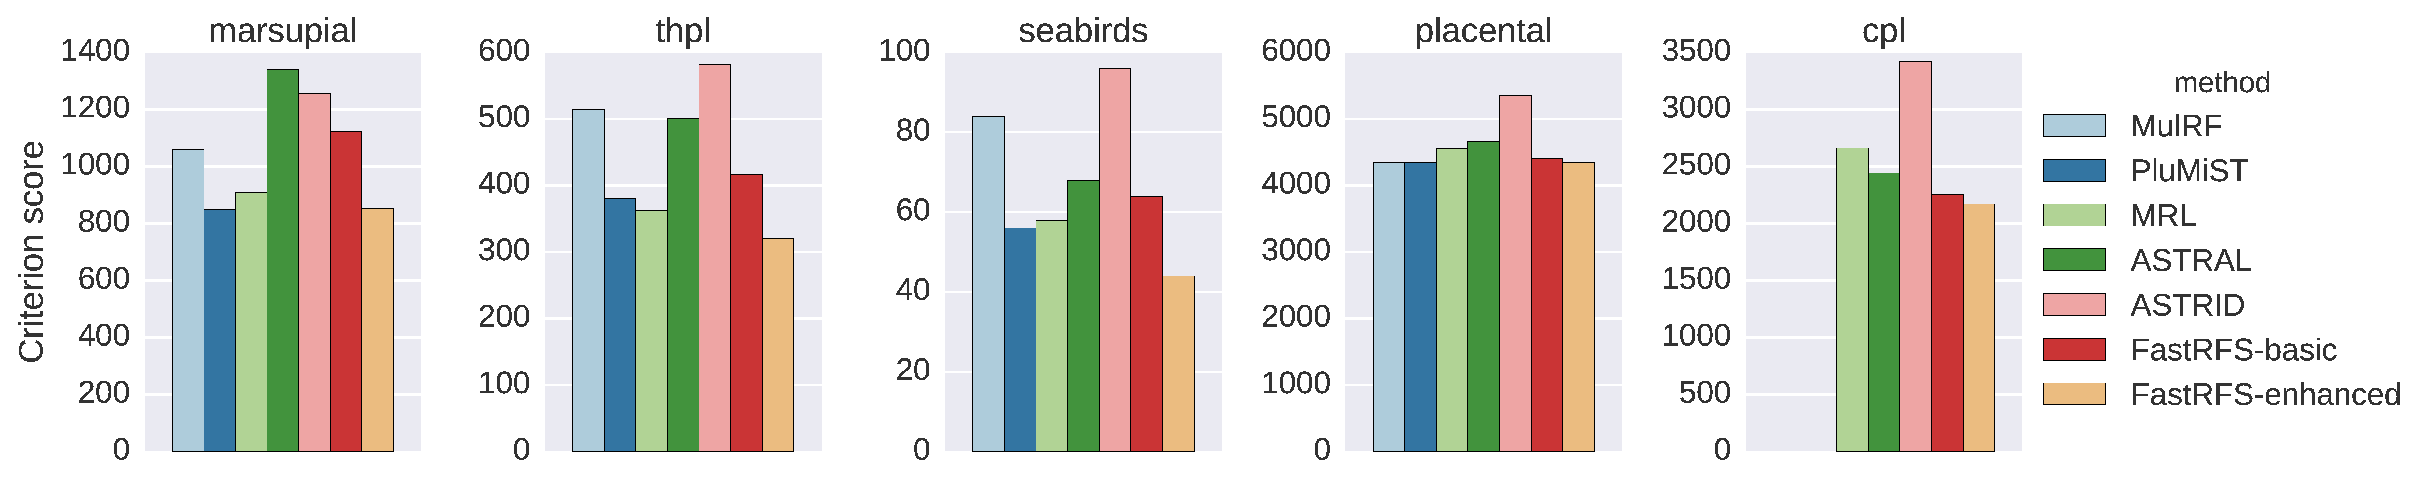
\includegraphics[width=\textwidth]{fastrfs-figs/bio-critscores.eps}
    \caption[Comparison of FastRFS and other supertree methods on five biological datasets with respect to RFS criterion score]{RFS criterion scores on biological data 
of supertree methods; lower is better.
MulRF and PluMiST could not be run on the CPL dataset due to its large size; hence
no values are shown for those methods on that dataset.
Overall, FastRFS-enhanced produces the best RFS criterion scores on these datasets.
}
    \label{fastrfs::fig:bio-critscores}
\end{figure}


 \begin{figure}
     \centering
     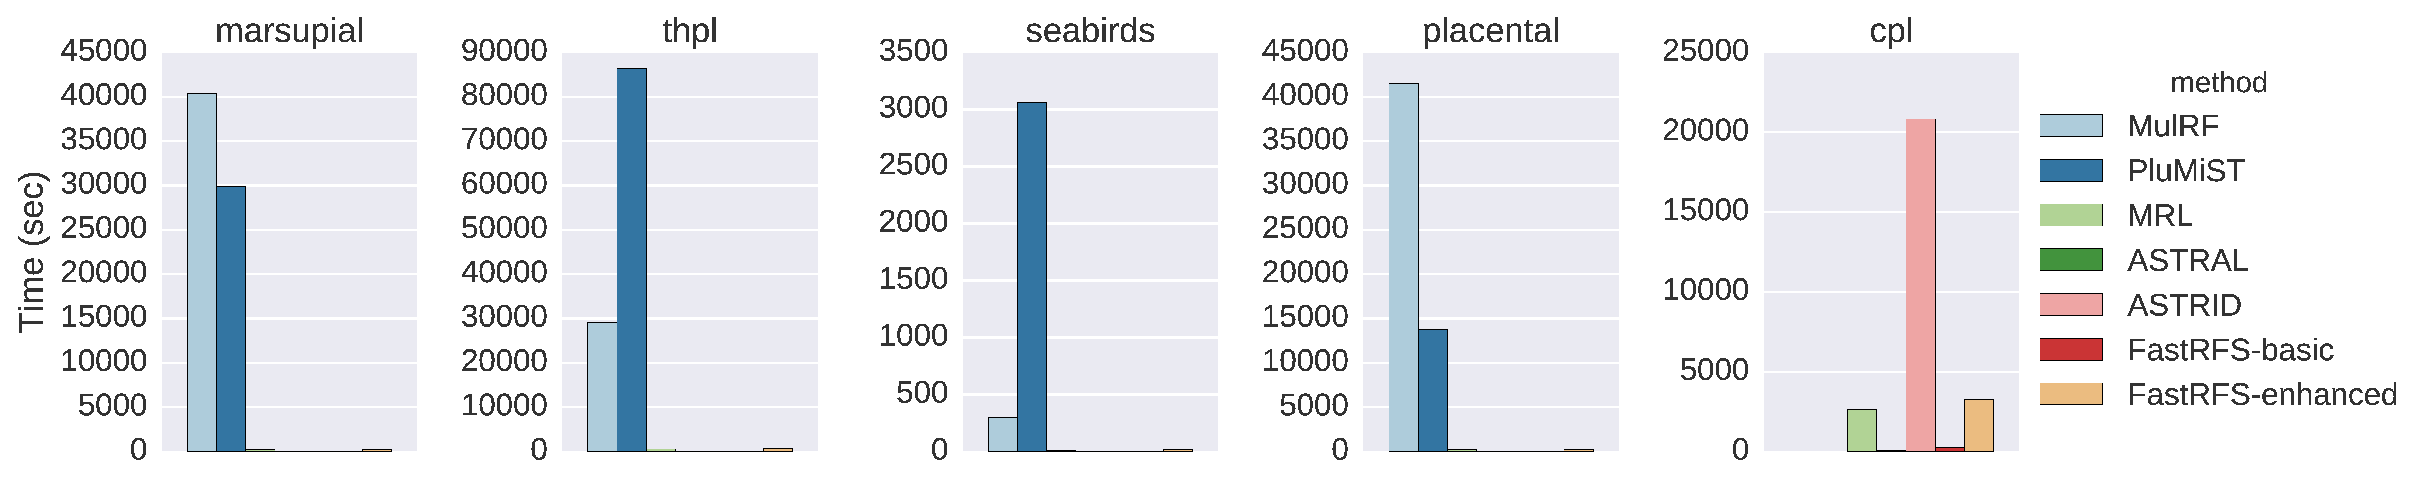
\includegraphics[width=\textwidth]{fastrfs-figs/bio-timing.eps}
     \caption[Running times of FastRFS and other supertree methods on five biological datasets]{Sequential running times (in seconds) on biological data of supertree methods. 
 MulRF and PluMiST could not be run on the CPL dataset, due to its large size; hence
 no values are shown for those methods on that dataset.
 }
     \label{fastrfs::fig:bio-timing}
 \end{figure}




\paragraph{\bf Datasets.  }
We used a collection of published simulated and biological datasets that
have been used in other studies \cite{smidgen} to evaluate supertree methods,
all of which are available online at
\url{http://www.cs.utexas.edu/users/phylo/datasets/supertrees.html}.

The simulated data, referred to as ``SMIDgen" in \cite{smidgen},
are generated
using  a taxon sampling strategy that mimics biological practice. 
These datasets have
100, 500, or 1000 taxa, with up to 25 source trees per replicate. 
Each supertree input has several ``clade-based" source trees and a ``scaffold tree", 
which are estimated using maximum likelihood heuristics on a concatenation 
of gene sequence alignments. 
Some genes are ``universal" and so are present in every species; others
evolve within the species tree under a birth-death model in which birth happens once but death (i.e., gene disappearance) can happen several times; therefore, unless the gene is born at the root of the species tree, it will be present only within a clade within the tree. Sequences then evolve down the gene trees under the GTRGAMMA model of site evolution.
The scaffold tree is based only on the universal genes, and have a random
subset of the species set; the clade-based trees are obtained by
selecting a clade in the tree and then a set of genes that covers
that clade well.
As shown in \cite{smidgen}, the density of the scaffold tree (i.e., the percentage of the full set of taxa that are in the scaffold dataset) has a large impact on the topological accuracy of the resultant estimated supertree.
 These simulated data enable us to evaluate topological accuracy as well as criterion score.
 
We include the biological datasets that were  also studied in
\cite{smidgen}:
CPL (comprehensive papilinoid
legumes) \cite{cpl},
Marsupials \cite{marsupial},
Placental Mammals \cite{placental},
Seabirds \cite{kennedy2002seabird}, 
and THPL (temperate herbaceous papilionmoid legumes) \cite{THPL}.
These range 
in size from 116 species (Placental
Mammals) to 2228 (CPL), and with
as few as 7 source trees (Seabirds) to as many as 726 (Placental Mammals).


\paragraph{\bf Methods.  }
In addition to the two FastRFS variants (basic and enhanced),
we computed supertrees using MRL, ASTRID, ASTRAL-2, MulRF, and PluMiST.
For 
MRL, 
we compute 
the MRP matrix using ``mrpmatrix" available at
\url{github.com/smirarab/mrpmatrix}, and we
use
RAxML \cite{RAxML} version 8.2.4
under the BINGAMMA model  with seed 12345 on the MRP matrix.
We ran 
MulRF version 1.2 \cite{mulrf} and
PluMiST version 1.1 \cite{plumist}.
We ran PluMiST in default mode, and we ran
MulRF ten times, and report results for the 
tree with the best criterion score.
We ran
ASTRAL-2 version 4.7.12  \cite{ASTRAL2} (henceforth
referred to as ASTRAL)
and
ASTRID version 1.1 \cite{ASTRID}, both in default mode.
Each of these methods produces fully resolved
unrooted trees.  


ASTRAL produces a supertree  that minimizes the total quartet distance
to the input source trees (equivalently, it produces a supertree that
maximizes the total quartet tree support) subject to a constrained
set $X$ of bipartitions that it computes from the input source
trees.

We tested an enhanced version of
ASTRAL (analogous to FastRFS-enhanced), in which 
we added the bipartitions from MRL and ASTRID 
to the set $X$; this enables a direct comparison of
FastRFS-enhanced and ASTRAL-enhanced. Although
FastRFS-enhanced is guaranteed to find RFS criterion scores
that are at least as good as
ASTRAL-enhanced, the comparison with respect to tree topology accuracy
makes it possible to evaluate the two optimization
criteria (minimize quartet distance or
minimize Robinson-Foulds distance) and their impact on topological accuracy.
Finally, we tested the impact of adding the bipartitions
from just one tree (MRL or ASTRID) to
the set $X$ on FastRFS, to determine the relative impact
of each additional tree.


\paragraph{\bf Measurements. }
We can use the simulated data to explore performance with respect to
criterion scores as well as tree estimation error. 
However, 
since there is no known true
supertree for the biological datasets, we use the biological 
datasets to explore performance only with respect to criterion scores.

For tree estimation error (explored only on the simulated
datasets), we
report the normalized bipartition distance (also
called the Robinson-Foulds error rate) between the
estimated and true trees.
The
Robinson-Foulds  (RF) error rate is
 $\frac{RF(T,T')}{2n-6}$, where $RF(T,T')$ is the RF distance between the true tree $T$ and the estimated tree $T'$, and $n$ is the number of leaves in $T$). 
Hence, the RF error rate is  between $0$ and $1$, and is equal to $0$ if and only if the two trees are identical. 

We also report the Robinson-Foulds Supertree criterion
score (i.e., the total Robinson-Foulds distance between the
estimated supertree
and the input source trees) for all datasets;
this value is bounded from
above by $(2n-6)k$, where $n$ is the total number of species and $k$ is the total number of source trees.

Although the criterion scores and tree error metrics both refer
to the Robinson-Foulds distance, the criterion score is based
on the RF distance to the input source trees, and the
tree error metric refers to the RF distance to the model  tree, which is unknown.
Hence these are two different ways of evaluating  methods.


Most of the methods are sequential codes; however, FastRFS is
parallelized to run on 8 cores and we run MulRF 10 times in parallel
and take the best tree.  We report wall clock running times for all
codes; except when the differences are large, comparisons between
running times are not reliable. Running times for FastRFS-enhanced
include the time to compute the MRL tree
and the ASTRID distance matrix, and, if the 
distance matrix has no missing data,   the time to run
FastME on the distance matrix (i.e., to fully compute the
ASTRID tree).

\paragraph{\bf Experiments.  }
We performed  experiments to evaluate the 
different supertree methods with respect to  
Robinson-Foulds criterion score,  topological accuracy of the supertree, and  
running time. 

\begin{table*}
\centering
\small
\begin{tabular}{|r|rrrrrrrrrrrr|}
\hline
Method&100 & 100 & 100 & 100 & 500 & 500 & 500 & 500 & 1000 & 1000 & 1000 &
1000\\
Scaffold \% &20 & 50 & 75 & 100 & 20 & 50 & 75 & 100 & 20 & 50 & 75 & 100\\
\# Replicates & 9 & 10 & 10 & 10 & 8 & 10 & 10 & 10 & 10 & 10 & 10 & 10 \\
\hline
\hline
ASTRAL& $\mathbf{11.7}$&$14.0$& $11.6$& $10.0$& $15.3$& $14.8$& $12.7$& $11.2$& $16.9$& $15.7$& $13.6$& $11.6$\\
ASTRAL-enh&$11.8$& $\mathbf{13.1}$&$11.5$& $10.0$& $14.8$&$14.1$& $12.6$& $11.2$& $\mathbf{16.3}$&$\mathbf{15.1}$&$13.5$&$11.6$\\
ASTRID& $15.8$& $18.7$& $17.1$&$9.6$&$26.0$& $50.1$& $45.4$&$\mathbf{10.5}$&$35.6$& $58.1$& $52.0$& $\mathbf{11.2}$\\
MRL&$13.6$& $13.6$& $11.2$& $10.8$& $15.4$& $14.3$& $12.1$& $11.2$& $17.4$&$\mathbf{15.1}$&$13.5$& $12.2$\\
MulRF&$22.1$& $26.0$& $15.3$& $9.3$&$46.9$& $40.3$& $27.4$& $12.6$& $-$&$-$&$-$&$-$\\
PluMiST&$25.9$& $16.6$& $11.5$& $9.3$&$35.4$& $29.5$& $22.4$& $10.9$&$-$&$-$&$-$&$-$\\
\hline
FastRFS-basic&$13.5$& $14.3$& $\mathbf{10.5}$&$\mathbf{9.1}$& $14.5$&$14.3$& $12.4$& $11.1$& $17.3$& $15.6$& $13.5$& $12.0$\\
FastRFS-enh&$13.5$& $13.4$& $10.6$& $9.3$&$\mathbf{14.3}$&$\mathbf{13.9}$&$\mathbf{12.0}$&$10.8$& $16.7$&$\mathbf{15.1}$&$\mathbf{13.4}$&$11.8$\\
\hline
\end{tabular}
  \caption[Supertree estimation error on simulated datasets for FastRFS and other methods]{Supertree topology estimation error on simulated datasets,
 measured using the Robinson-Foulds error rate, expressed
as a percentage.
The best result for each model condition is boldfaced. No results are shown
for PluMiST or MulRF on the 1000-taxon simulated datasets due to
running time limitations for these methods.
Results are averaged over the completed replicates. }
  \label{fastrfs::table:exp1-topo}
\end{table*}




\section{Results and Discussion}
\label{fastrfs::sec:results}

\paragraph{Impact of the constraint set on criterion scores. }
Our initial experiment evaluated the impact on the
criterion scores found by FastRFS of
adding bipartitions from the MRL tree and/or the ASTRID tree to the constraint
set.
In general, FastRFS with the MRL tree alone added
was nearly as good as FastRFS-enhanced (i.e.,  with both 
ASTRID and MRL trees added), and FastRFS with MRL found substantially
better criterion scores than
FastRFS with just the ASTRID tree added.
Nevertheless, since adding
the ASTRID tree did help occasionally, and since ASTRID is so quick to
run when the distance matrix is complete, we continued using it for
FastRFS-enhanced.
See Figures \ref{fig:fastrfs-sup::sim-fastrfs-comp} and \ref{fig:fastrfs-sup::bio-fastrfs-comp} for these results.


\paragraph{Criterion scores for the simulated datasets. }

By design, FastRFS-enhanced will always find criterion scores
that are at least as good as those found
by ASTRAL-enhanced, FastRFS-basic, ASTRAL, and MRL.
Hence, the only methods that could possibly find
better scores than FastRFS-enhanced are PluMiST, MulRF,
and ASTRID. 
We show the Robinson-Foulds Supertree criterion scores
in Table \ref{fastrfs::table:simulated-critscores}; note that
lower is better.
PluMiST failed to complete
on three datasets (one replicate  in the 
100-taxon and two replicates in the 500-taxon
datasets, each with 20\%-scaffolds); we report
results only on the remaining datasets. 
Both PluMiST and MulRF had very large
running times on the 500-taxon datasets; therefore, 
we did not
attempt to run them on the 1000-taxon datasets.
All other methods succeeded in completing on all
datasets we examined.

FastRFS-enhanced found the 
best (lowest) Robinson-Foulds Supertree
(RFS)
criterion scores of all methods for
all datasets; FastRFS-basic also found
these best scores for three of the four 100-taxon
model conditions, but otherwise found higher scores.
PluMiST found better RFS 
criterion scores than MulRF in 7 of the 8
model conditions, and  matched in 1 condition.
ASTRID had the worst performance of all methods,
with much larger criterion scores on all
the sparse scaffold model conditions.
These are the same conditions in which 
the internode distance matrix has missing entries, 
suggesting that
the reduced accuracy is largely due to the missing data in
the distance matrix.

Certain additional trends are worth noting.
First, although PluMiST did well on the 100-taxon
datasets, it was not so competitive with FastRFS-enhanced
or even FastRFS-basic on the 500-taxon datasets, suggesting
that 
the number of taxa may impact the ability of
PluMiST to find trees with good criterion scores.
ASTRAL-enhanced matched or improved on the
RFS criterion scores compared
to ASTRAL; this is interesting because it
does not follow from the algorithm design
(the two methods seek the tree that minimizes
the quartet distance, not the RFS criterion).
MRL, although never coming in first, often
had very good results, coming just behind
FastRFS-basic for overall performance. 








\paragraph{Criterion scores on biological datasets. }

We were unable to 
run PluMiST and MulRF on the CPL dataset, the largest
in our collection, due to its size: at 2228 species,
the running time needed for these two methods is
excessive.
Criterion scores on the biological datasets follow 
very similar patterns as observed on the simulated 
datasets (Fig.~\ref{fastrfs::fig:bio-critscores}). %(Fig.  2). %\ref{fastrfs::table:bio-rfscore}), Tandy hardwired
Overall, FastRFS-enhanced had the
best criterion scores: the best on
four datasets, and close to best on the last
dataset (Marsupials).
PluMiST tied for best with FastRFS-enhanced
on two  of the four
datasets on which it can run, 
had the second best score on seabirds,
and third best on THPL.
Hence, PluMiST is in second place.
Interestingly, the dataset on which PluMiST was
not able to find one of the top two scores
was the second largest dataset, with more
than 500 species.
Thus, just as we 
saw on the simulated datasets, the number of species seems to impact
the relative performance of PluMiST in comparison
to other methods.

The next two best methods are MRL and FastRFS-basic,
which had close performance, but MRL was
slightly better.
ASTRAL and MulRF are next, again with
mixed performance (MulRF was better
on two datasets and ASTRAL was better on the other
two). Finally, ASTRID had the worst
performance of all methods - coming in 
dead last on four of the five datasets.
It is worth noting that all but two of
the datasets produced distance matrices
with missing entries, and ASTRID did better
than ASTRAL on one 
of the two datasets (marsupial)
that produced a complete distance matrix.








\paragraph{Topological accuracy.  }
Since the true supertree is not known for the biological datasets, 
we evaluate topological accuracy only on the simulated datasets
red
(Table 2).
All methods improved in accuracy with the increase
in the scaffold density, so that error rates were
generally highest for 20\%-scaffolds and lowest
for 100\%-scaffolds.
The differences between methods on the 100\%-scaffolds
were generally small, but there were large differences
under the other conditions.
ASTRID had very 
poor accuracy except for those with
100\%-scaffolds, and MulRF and PluMiST also
had poor accuracy with the lower density scaffolds.

The remaining methods (MRL, the two ASTRAL versions, and the
two FastRFS versions)
were fairly close in accuracy.
However, MRL was never more
accurate than FastRFS-enhanced, and was only the top
performing method for one model condition 
(where
it tied with FastRFS-enhanced).
ASTRAL-enhanced was more accurate than ASTRAL on 8 conditions,
tied on 1 condition, and less accurate on 3 conditions.
FastRFS-enhanced was more accurate
than FastRFS-basic on 9 model conditions,
tied on 1 condition, and worse on 2 conditions.
FastRFS-enhanced was more accurate than
ASTRAL-enhanced on 8 
of the 12 model conditions, tied on
1 condition, and worse on 3 conditions.

FastRFS-enhanced was the
top performing method on 5 of the 
12
model conditions; the next
best performing method
was ASTRAL-enhanced, which was the top
performing method in 3 of the 12 model conditions.
Thus, overall FastRFS-enhanced provided
the best accuracy of the tested supertree methods.
These results, and especially the
pairwise comparisons,  suggest that
optimizing the Robinson-Foulds Supertree
criterion (minimize RF distance) is better than
optimizing the ASTRAL criterion (minimize
quartet distance) for supertree estimation, and
that adding bipartitions from MRL (and 
from ASTRID if its internode distance matrix
is complete) also tends to improve accuracy.

\paragraph{Running time. } 





Figure \ref{fastrfs::fig:bio-timing} 
shows running times on the biological datasets.
MulRF and PluMiST took the most time,
 each typically requiring
hours where FastRFS-basic, MRL, and ASTRAL completed in 
well under a minute (and sometimes in just a few seconds).
MRL and FastRFS-enhanced were the next most computationally 
intensive, but were
sometimes
fast, and finally 
ASTRAL, ASTRID, and FastRFS-basic were the fastest,
often completing in just seconds. 
As an example, 
the running times on the largest dataset on which
all the methods completed
(THPL, with 558 taxa) showed substantial
differences between methods:
PluMiST used 86400 seconds (i.e., 24 hours), MulRF
used 29160 seconds (i.e., 8.1 hours), 
FastRFS-enhanced used 615 seconds (just over 10 minutes), 
MRL used 575 seconds (i.e., just under 10 minutes),
and ASTRID, ASTRAL, and FastRFS-basic used under 20 seconds.

The size of $X$ impacts the running time for FastRFS, and
ranged from 1155 to 
20,233 for FastRFS-basic
and from 2485 to 48,313 for FastRFS-enhanced.
The most computationally intensive dataset
for FastRFS-enhanced is the CPL dataset, which maximizes
both the number of taxa and $|X|$; 
however, FastRFS-enhanced
completed on this dataset in 
3282 seconds (i.e., 
under an hour).
The majority of the time for FastRFS-enhanced is spent
computing the MRL tree; the other parts of the analysis 
(i.e., computing the ASTRID matrix and potentially the ASTRID
tree, computing the constraint set from ASTRAL, and running the DP
algorithm) takes very little time (typically less than a minute).


ASTRID's running time was highly variable,
but the running time is high only for
large datasets with missing entries in the
distance matrix. The reason is
that when the matrix has missing entries, ASTRID must use BIONJ*
(which takes $\Theta(n^3)$ time)
instead of FastME (which takes $\Theta(n^2)$ time).
For example, ASTRID used about 6 hours
on the CPL dataset (the only biological
dataset with these missing entries), 
but completed in just seconds on all the other
datasets. %On the CPL dataset, the ASTRID distance matrix is missing
%entries, so ASTRID uses BIONJ*, which takes $\Theta(n^3)$ time,
%instead of FastME, which takes $\Theta(n^2)$ time. 
%This is extremely
%time consuming on datasets with many taxa, like the CPL dataset, which
%has 2228 taxa.

















\section{Conclusions}


Supertree estimation is a basic bioinformatics challenge that 
is necessary for the construction of large phylogenies as well 
as for enabling statistical phylogeny estimation methods to be applied to large datasets. 
While many methods have been developed to compute supertrees, very few have
been able to provide good accuracy on datasets with many hundreds or thousands
of species.

The FastRFS methods presented
here (i.e., the basic and enhanced versions) are fast and effective techniques 
to find solutions 
to the  NP-hard Robinson-Foulds Supertree (RFS) problem.
FastRFS-enhanced in particular nearly always finds better
solutions than PluMiST and MulRF, the leading
methods for RFS,
and does so 
 in much less time.
FastRFS relies upon a dynamic programming algorithm to find an 
exact solution to its optimization problem within a constrained search space,
a strategy introduced in 
\cite{hallett2000new}
and that  is
quite different from
the heuristic search
techniques used by most phylogeny estimation methods. 
Thus, while  FastRFS, PluMiST, and MulRF all seek to optimize the same criterion, 
FastRFS is guaranteed to find an optimal solution within its constraint space but cannot return any tree that is not within the constraint space, while PluMist and MulRF are not guaranteed to find an optimal solution within any search subspace but have access to the entire treespace. 
Thus, our study suggests that
  exactly solving
an optimization problem within a constrained search space
may be a better approach than being able to search a larger space,
as long as the constrained space is selected carefully.
However, our study also shows that expanding the constraint
set beyond the input set of source trees can be highly beneficial
in terms of finding good solutions to NP-hard optimization
problems.

FastRFS-enhanced also tends to find more accurate
tree topologies than the other supertree methods
we explored. 
The improvement in topological accuracy
suggests that 
the Robinson-Foulds Supertree problem is
a good approach to supertree estimation.
The explanation for this
is likely to be the 
close relationship between the Robinson-Foulds
Supertree problem and 
the Maximum Likelihood Supertree problem
\cite{BryantSteel2009}, which
models source tree discord based on the topological distance
to the true supertree
\cite{ml-supertree}.
Thus, although a Robinson-Foulds
Supertree is not guaranteed to be identical
to a Maximum Likelihood Supertree,
good solutions to one problem are likely to be good
solutions to the other \cite{BryantSteel2009}.
Hence, 
FastRFS 
may be a good heuristic for the Maximum 
Likelihood Supertree problem,
and this may explain its good accuracy.    

There are many directions for future work.
For example, since FastRFS by design can only
search 
within the space defined by its constraint set,
finding better constraint sets may provide additional
improvements. Alternatively, FastRFS-enhanced
may provide a good starting tree
for PluMiST and MulRF, which are able to search
an unconstrained search space.
In addition, FastRFS-enhanced may be a good
initial tree for 
Bayesian supertree methods \cite{Akanni-HGT,Akanni-Bayesian} or 
heuristic searches for Maximum Likelihood Supertrees
 \cite{Akanni-MLsupertree}.
Also, like most
supertree methods, FastRFS currently only works with 
inputs where each source
tree has at most one copy of each leaf;
methods like MulRF are designed to handle inputs of  source trees
that represent gene trees, and so can
have multiple copies of each species (arising from duplication-loss
scenarios).
We will modify  FastRFS to be able to work with
such source tree inputs.


\section{Supplementary Data for FastRFS}

\subsection{Size of the constraint set}

%Increasing the size of the constraint set $X$ impacts the running time,
%tree topology accuracy, and criterion scores for FastRFS-enhanced and 
%ASTRAL-enhanced. 
FastRFS-enhanced uses a larger constraint space than FastRFS-basic.
Table \ref{tab:set-x} shows the sizes of the constraint sets $X$ for
the five biological datasets that are added to the search spaces for
FastRFS-enhanced and ASTRAL-enhanced.

\begin{table*}
  \centering
  \begin{tabular}{c|rrrrr}
    Method             & Seabirds & Placental & Marsupial & THPL & CPL
    \\
    \hline 
    FastRFS-basic      & 1155     & 6907      & 10251     & 11109&
                                                                   20233
    \\
    FastRFS-enhanced      & 2485     & 12937      & 15443     & 17811&
                                                                   48313 \\    
  \end{tabular}
  \caption{Sizes of the set $X$ on biological datasets}
  \label{tab:set-x}
\end{table*}



\subsection{Commands}

Commands for the tree estimation software are provided below:

\paragraph{MulRF: }
We ran MulRF version 1.2 ten times,  and the tree with the
best optimization score was used. The command was:
\begin{verbatim}
MulRFSupertree -i <input file name> -o <output file name>
\end{verbatim}

\paragraph{PluMiST: }
We ran PluMiST version 1.1.  Since we found PluMiST's stopping
condition caused it to run for too long, we allowed PluMiST to run for
a limited amount of time (1 hour for 100-taxon simulated dataset; 5
hours for 500-taxon simulated dataset; 12 hours for the the seabird,
mammalian, and placental datasets, and 24 hours for the THPL
dataset). In all cases, this was at least as long as the other methods
took to run and in most cases substantially longer. Reported running
times are the times of the last iteration that successfully completed
before the cutoff. The command used for PluMiST was
\begin{verbatim}
python plumist.py -s <input file name> -o <output file name>
\end{verbatim}


\paragraph{MRL: }
We also ran matrix representation with likelihood (MRL), in which a
maximum-likelihood tree is estimated on an MRP matrix. We generated
MRP matrices with mrpmatrix, available at
\url{github.com/smirarab/mrpmatrix}:
\begin{verbatim}
mrpmatrix <input file> <output matrix file> -dna
\end{verbatim}
We estimated MRL trees with RAxML version 8.2.4 with command line 
\begin{verbatim}
RAxML -m BINGAMMA -p 12345 -n <run name> -s <matrix file>
\end{verbatim}

\paragraph{ASTRID:}
To run ASTRID, we used the command line
\begin{verbatim}
ASTRID -i <gene tree file> -o <output file>
\end{verbatim}

\paragraph{ASTRAL:}
To run ASTRAL, we used the command line
\begin{verbatim}
java -jar astral.4.7.8.jar -i <gene tree file> -o <output file>
\end{verbatim}
To run ASTRAL-enhanced, we used
\begin{verbatim}
java -jar astral.4.7.8.jar -i <gene tree file> -o <output file> -e
<extra trees>
\end{verbatim}
where the extra trees file contained the MRL tree or the MRL tree and
the ASTRID tree, depending on whether or not the ASTRID distance
matrix was complete.

\paragraph{FastRFS-basic: } 
To run FastRFS, we used the command line
\begin{verbatim}
wASTRAL -c FastRF  -g <gene tree file> -o <output file>
-a /path/to/astral.4.7.8.jar
\end{verbatim}

\paragraph{FastRFS-enhanced: }

To run the enhanced version of FastRFS, we used the
command line
\begin{verbatim}
wASTRAL -c FastRF  -g <gene tree file> -o <output file>
-a /path/to/astral.4.7.8.jar -e <extra trees> --extraextra
\end{verbatim}
%TODO: describe this
This runs the clade selection portion of ASTRAL three times to get the
constraint set. First, it runs with the input trees as gene trees and
the extra trees as extra trees. Second, it runs with the extra trees
as the gene trees. Finally, it runs with input and extra trees
combined as gene trees. The union of these outputs is used as the
clade set for FastRFS.
\clearpage

 \begin{figure*}
   \centering
   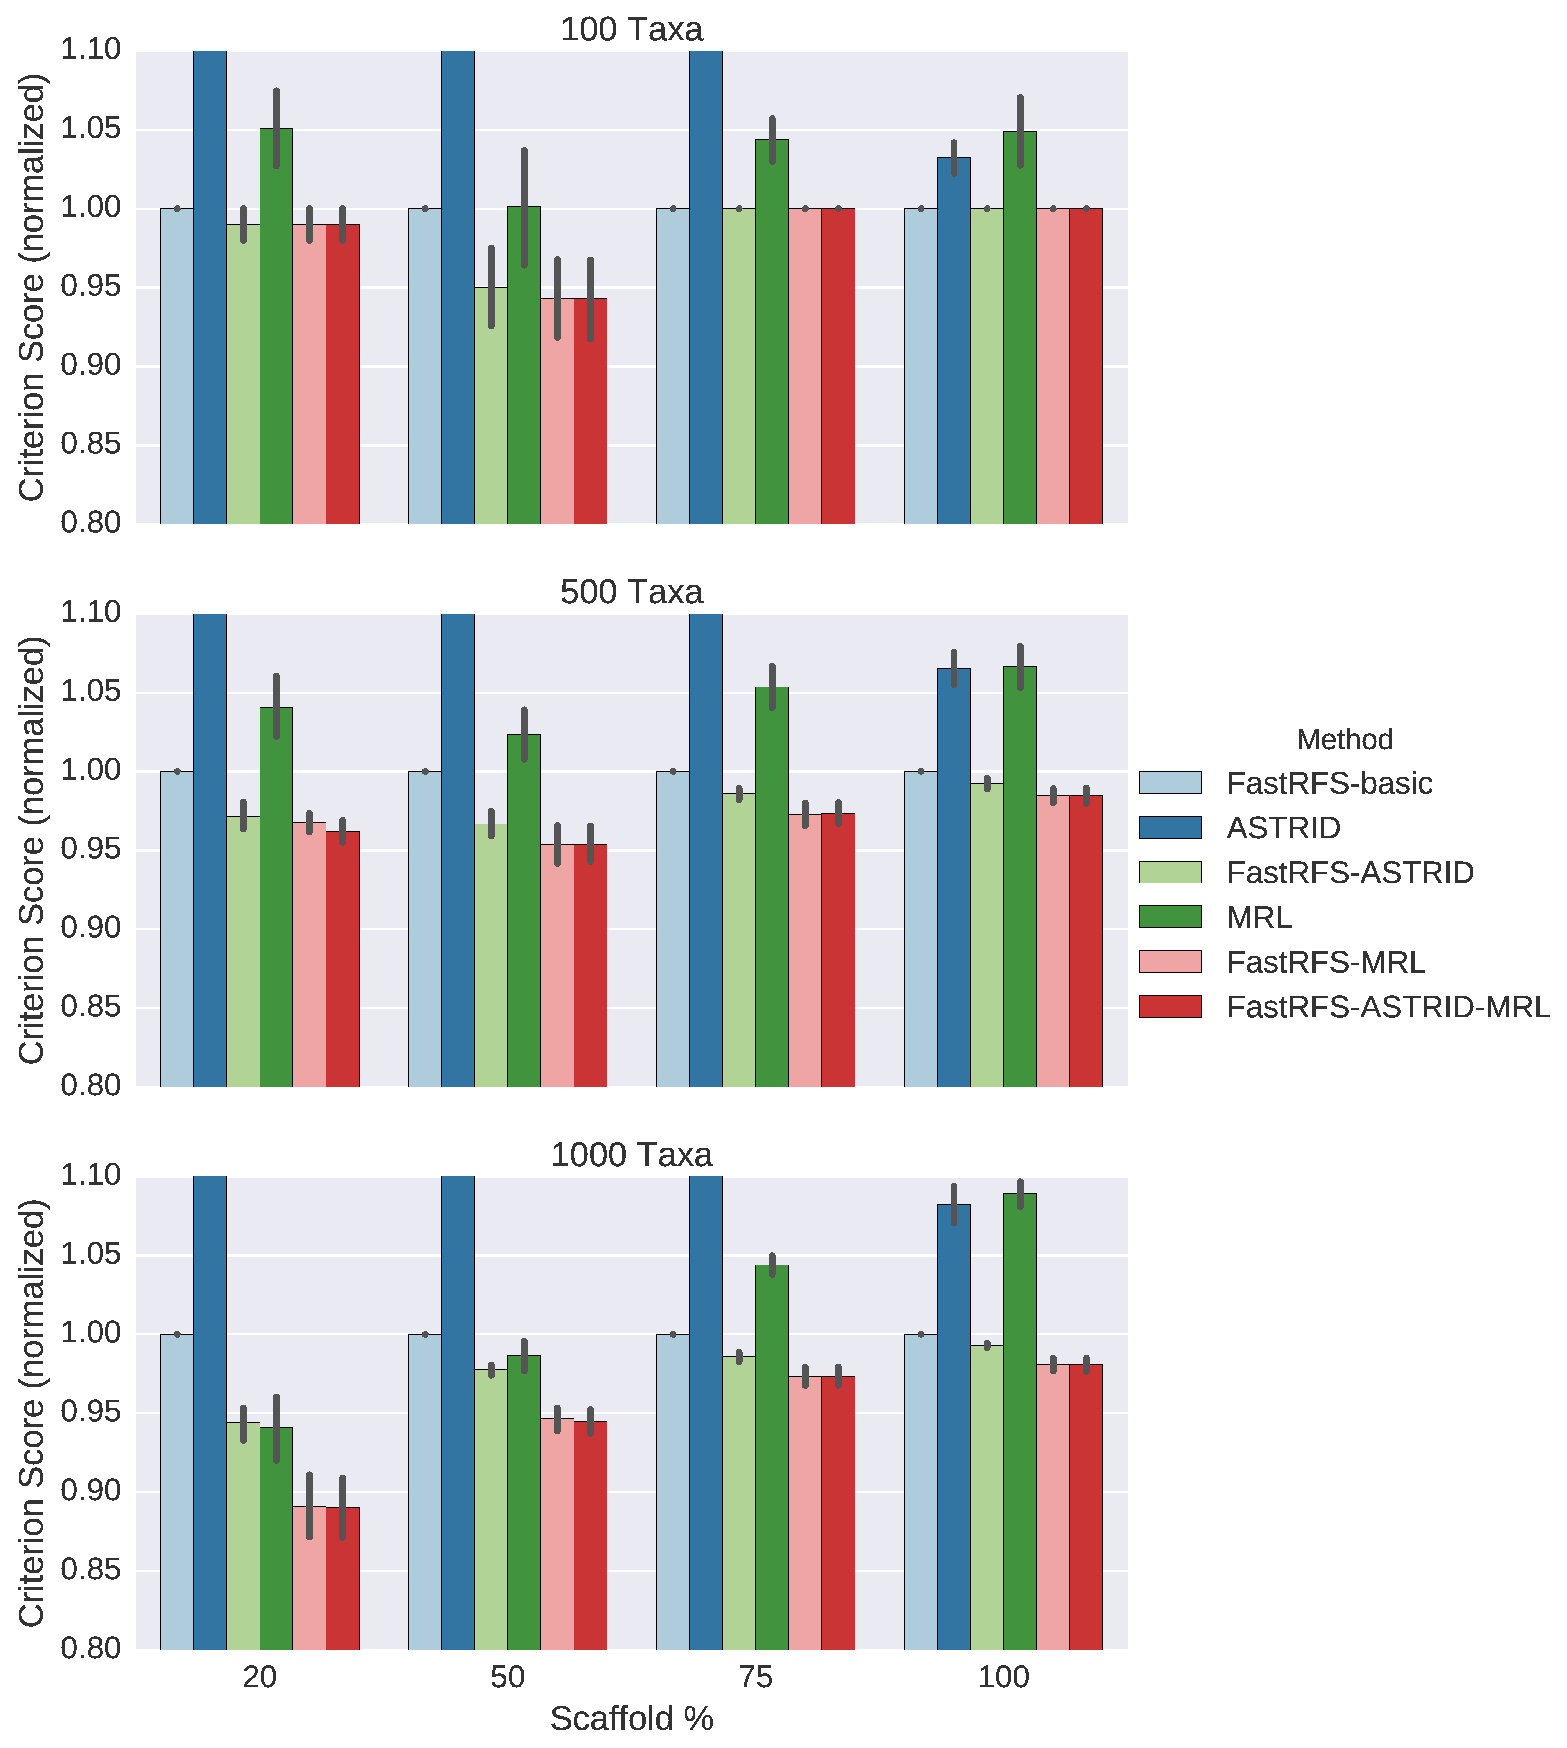
\includegraphics[width=\textwidth,height=0.6\textheight,keepaspectratio]{fastrfs-figs/smidgen-critscores-fastrfs-comparison.eps}  
   \caption{Comparison of FastRFS variants criterion scores on
     simulated data. Scores are normalized by dividing by the
     FastRFS-basic score; FastRFS-basic has a score of 1.}
   \label{fig:fastrfs-sup::sim-fastrfs-comp}
 \end{figure*}


 % \begin{figure*}
 %   \centering
 %   \includegraphics[width=\textwidth]{../../rfsupertree/analysis/smidgen-err-fastrfs-comparison}  
 %   \caption{Comparison of FastRFS variants topological errors on
 %     simulated data.}
 %   \label{fig:sim-fastrfs-comp}
 % \end{figure*}



 % \begin{figure*}
 %   \centering
 %   \includegraphics[width=\textwidth]{../../rfsupertree/analysis/smidgen-timing-fastrfs-comparison}  
 %   \caption{Comparison of FastRFS variants running times on simulated
 %     data. This does not take into account the additional time needed
 %     to run ASTRID and MRL. }
 %   \label{fig:sim-fastrfs-comp}
 % \end{figure*}


 \begin{figure*}
   \centering
   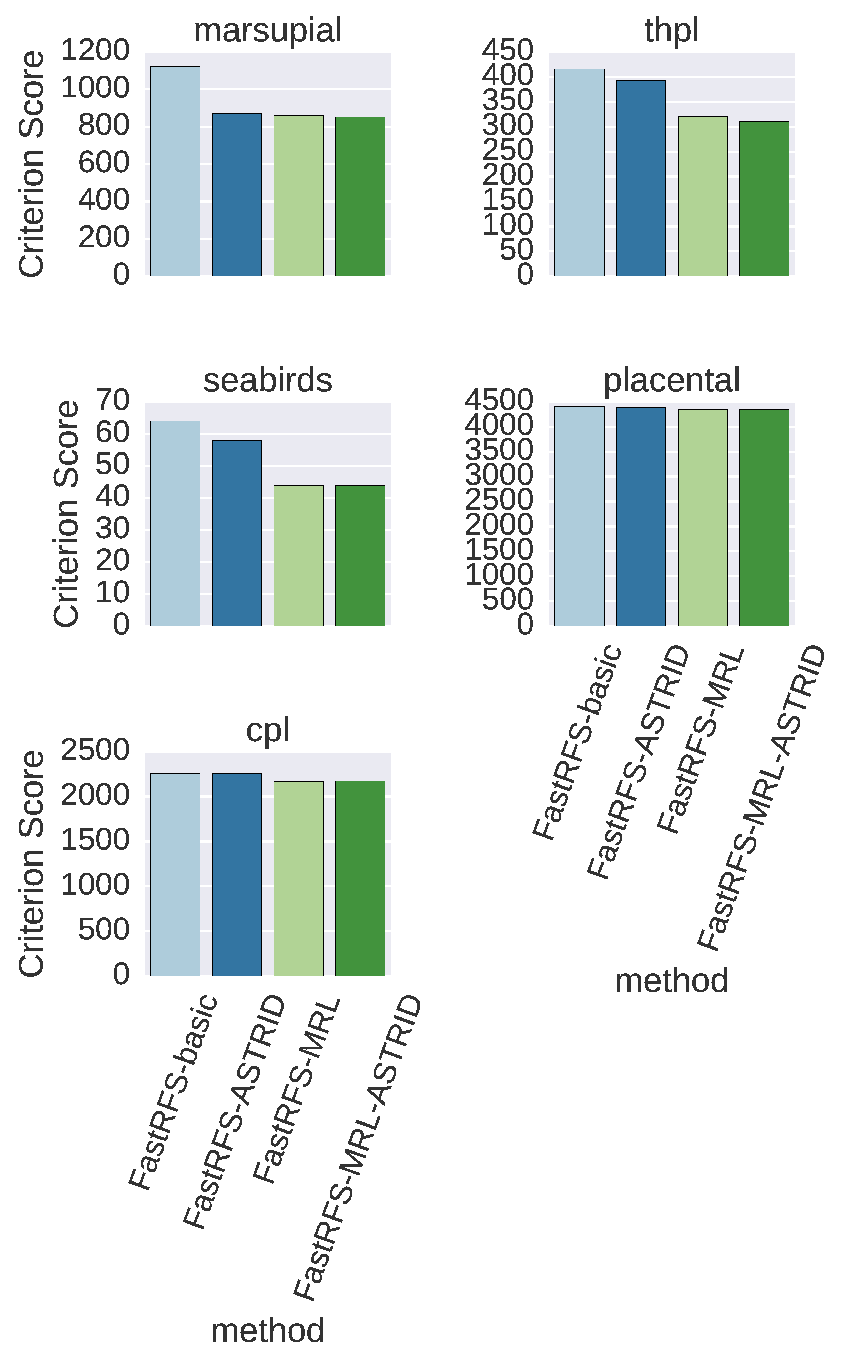
\includegraphics[width=\textwidth,height=0.9\textheight,keepaspectratio]{fastrfs-figs/bio-rfscores-fastrfs-comp.eps}
   \caption{Comparison of FastRFS variants on biological data}
   \label{fig:fastrfs-sup::bio-fastrfs-comp}
 \end{figure*}


\end{document}

\chapter[Improving Dynamic Programming for Phylogenomic Estimation
  with SIESTA]{Improving Dynamic Programming for Phylogenomic Estimation
  with SIESTA\protect\footnotemark}\footnotetext{This chapter contains material previously published in \cite{vachaspati2018siesta}, which was a joint work with Tandy Warnow. It has been edited slightly for brevity. PV implemented SIESTA, performed experiments, wrote the first draft, and analyzed the data. TW analyzed the data, and wrote the final draft.}
\label{chapter:siesta}


\section{Background}
\label{siesta::sec:intro}
% Phylogeny estimation is generally approached as a statistical estimation problem, and finding the best tree for a given dataset is typically based on methods that are computationally very intensive; for example, maximum likelihood phylogeny estimation is NP-hard \cite{roch2006short} and Bayesian MCMC methods require a long time to converge. 
% For this reason, among others, the calculation of very large phylogenies is often enabled by divide-and-conquer methods that use  ``supertree methods" to combine smaller trees into larger trees.
% A more common use of supertree methods is to combine trees computed by independent research groups on different datasets into a single tree on a large dataset \cite{bininda2004phylogenetic}. 
% While Matrix Representation with Parsimony (MRP) \cite{baum-mrp,ragan-mrp} is the most well known supertree method, other  supertree methods have been shown to have better accuracy than MRP (e.g., Matrix Representation with Likelihood \cite{nguyen2012mrl}, FastRFS \cite{vachaspati2017fastrfs}, and the recently proposed Bad Clade Deletion  supertree method \cite{fleischauer2017bad}). 
% Supertree methods are an area of active research in the computational phylogenetics community, with new methods introduced frequently and used in a variety of contexts \cite{Akanni-Bayesian,holder-redelings-supertree,lafond-supertree-2017}.

% Species tree estimation, even for small numbers of species, is also difficult because of multiple processes that create differences in the evolutionary history across the genome; examples of such processes include  incomplete lineage sorting (ILS), gene duplication and loss (GDL), and horizontal gene transfer (HGT) \cite{maddison1997gene}. 
% Species tree estimation is therefore performed using multiple loci from throughout the genomes of the different organisms, and is referred to as ``phylogenomics''.
% One of the standard approaches for species tree estimation is to compute gene trees (i.e., trees on different genomic regions) and then combine the trees together into a species tree under statistical models of evolution, such as the multi-species coalescent (which models ILS), that allow for gene tree heterogeneity. 
% Examples of   such ``summary methods" (i.e.,  methods that construct species trees by combining gene trees) that are statistically consistent under the multi-species coalescent model  include ASTRAL \cite{mirarab2014astral,mirarab2015astral,astral3}, GLASS \cite{mossel2010incomplete},
% the population tree in BUCKy \cite{larget2010bucky},
% MP-EST \cite{Liu2010a},  
% NJst \cite{liu2011estimating}, and a modification of NJst called ASTRID \cite{Vachaspati2015-ASTRID}.

% Summary methods  share algorithmic features in common with supertree methods in that both construct trees on the set of species by combining trees on subsets of the species set; the difference between the two types of methods is that in the supertree context, the assumption is that the heterogeneity observed between these ``source trees" is due only to estimation error, while in the phylogenomic context the assumption is that source trees can differ from each other and from the species tree due to a combination of estimation error and true heterogeneity resulting from ILS, GDL, HGT, or some other causes. 
Coalescent-aware summary methods and supertree methods are often based on attempts to solve NP-hard problems, and typically use heuristics  (a combination of hill-climbing and randomization) to search for optimal trees.
While these heuristics can be highly effective on small datasets, they are often very slow 
and there are no guarantees about the solutions they find.
An alternative approach to the use of heuristic searches is constrained exact optimization, whereby the solution space is first constrained using the input source trees, and then  an exact solution  to the optimization problem is found within that constrained space.
This approach can lead to polynomial time methods (where the running time depends on the size of the constraint space as well as on the input) that can have outstanding accuracy.
The first use of this approach was presented in   \cite{hallett2000new}, which provided a method to find a species tree minimizing the duplication-loss reconciliation cost given a set of estimated gene trees. 
Since then, many other constrained exact optimization methods have been developed in phylogenomics for different purposes, including  computing trees from maximum likelihood quartet trees \cite{bryant2001constructing}, constructing species tree  from sets of gene trees under gene duplication and loss models  \cite{bayzid2013inferring} or under the multi-species coalescent model \cite{ThanNakhleh2009,yu2011algorithms,mirarab2014astral,mirarab2015astral}, improving gene trees given a species tree  \cite{szollosi2013efficient}, constructing consensus trees \cite{bryant2001constructing}, 
constructing supertrees \cite{vachaspati2017fastrfs},  and extracting a tree from a phylogenetic network \cite{bryant2001constructing}.

 

Most of these  approaches constrain the search space using  a set of ``allowed bipartitions", which we define here.
% Each edge $e$ in an unrooted tree $T$ on a set $S$ of species defines a bipartition $\pi_e$  of $S$ (also called a ``split"), obtained by deleting $e$ but not its endpoints from $T$; hence, every tree $T$ can be defined by its set of bipartitions $Bip(T) = \{\pi_e: e \in E(T)\}$.
The constraints imposed by these algorithms are obtained by specifying a set $X$ of allowed bipartitions so that the returned tree $T$ must satisfy that $Bip(T) \subseteq  X$.
The set $X$ is used to define a set of ``allowed clades'' (comprised of the halves of the bipartitions, plus the full set of species), and dynamic programming is then used on the set of allowed clades  to  find an optimal solution to the optimization problem.  
The set $X$ has an impact on the empirical performance, but even simple ways of defining $X$ can result in very good accuracy and provide guarantees of statistical consistency under statistical models of evolution \cite{mirarab2015astral,vachaspati2017fastrfs}.

The constrained exact optimization approach has multiple advantages over heuristic search techniques. 
From an empirical perspective, the dynamic programming approach is frequently faster, and if the constraint space is selected well it is often more accurate than alternative approaches that typically use heuristic searches for optimal solutions.
From a theoretical perspective, the ability to provably find an optimal solution within the constraint space is often sufficient to prove statistical consistency under a statistical model of evolution (e.g., under the multi-species coalescent model); hence, many of the methods that use constrained exact optimization can be proven statistically consistent, even for very simple ways of defining the constraint set. 

These constrained exact optimization methods typically have excellent accuracy in terms of  scores for the optimization problems they address (established on both biological and simulated datasets) and topological accuracy of the trees they compute (as established using simulated datasets).
A basic limitation of these methods, however, is that they return a single optimal tree, even though there can be multiple optima on some inputs.
This limitation reduces the utility of the methods.


We present SIESTA (Summarizing Implicit Exact Species Trees Accurately), an algorithmic tool that can be used to enhance these dynamic programming methods for finding optimal trees. 
The input to SIESTA is the set $\mathcal{T}$ of source trees, the constraint set $X$ of allowed bipartitions, and a scoring function $w$ that assigns scores to tripartitions of the taxon set (and which is derived from the optimization function $F$ that assigns scores to trees and the set $\mathcal{T}$, as we show later); SIESTA  returns a  data structure $\mathcal{I}$ that represents the set $\mathcal{T}^*$ of trees that optimize the function $F$ subject to the constraint that every bipartition in every tree in $\mathcal{T}^*$ is in $X$. 
This data structure $\mathcal{I}$ enables the user to explore the set of optimal trees in various ways. 
In this study, we use SIESTA to compute consensus trees, to enumerate the set of optimal trees,
to count the number of optimal trees,  and to report the frequency of each bipartition in the set of optimal trees.  

We explore the impact of using SIESTA with  two methods that use  dynamic programming  for constrained exact optimization: the supertree method FastRFS  \cite{vachaspati2017fastrfs} and the ILS-aware species  tree estimation method ASTRAL \cite{mirarab2015astral}.
We show that using SIESTA to compute a strict consensus tree provides improvements in accuracy (in terms of the topology of the estimated tree) compared to a single optimal tree for both ASTRAL and FastRFS when the number of optimal trees is large enough, and is otherwise neutral.  
Furthermore, using SIESTA with a modification to FastRFS produces more accurate rooted supertrees than Bad Clade Deletion (BCD), the previous best method for rooted supertree construction \cite{fleischauer2017bad}. 

Using SIESTA with ASTRAL, a species tree estimation method that addresses incongruence due to ILS, provides additional benefits.
For each optimal  tree it returns, ASTRAL provides branch support values based on local posterior probabilities, but these values do not take the other optimal trees into account.
We show how to correct these support values   to take the full set of optimal ASTRAL trees into account, and enable the calculation of a maximum clade credibility (MCC) tree based on these corrected values.
Hence, SIESTA provides a valuable tool for both species tree and supertree estimation, providing distinct advantages over the simplistic use of  leading methods for these problems.
SIESTA, combined with ASTRAL and FastRFS  is available at
https://github.com/pranjalv123/SIESTA and
the datasets analyzed in this paper are available at \cite{siesta-data}.


\section{Methods}

\subsection{The SIESTA Algorithm}

SIESTA is designed to work with tree estimation methods that seek optimal solutions within a constrained search space using dynamic programming. 
Recall that in the constrained optimization approach, the input  is a set of source trees (estimated gene trees in the case of ASTRAL, generic source trees in the case of FastRFS) as well as a set $X$ of allowed bipartitions of the set $S$ of species.
Given this set $X$ of allowed bipartitions, we define a set $\mathcal{C}$ of ``allowed clades" by taking the two halves of each bipartition, and we also include the set $S$; thus, $\mathcal{C} = \{A: [A|S \setminus A] \in X \} \cup \{S\}$.

We also form a set $\mathop{\rm TRIPS}$ of ``allowed tripartitions", as follows. 
$\mathop{\rm TRIPS}$ contains all ordered 3-tuples $(A,B,C)$ of allowed clades that are pairwise disjoint, that union to $S$, and where $A \cup B$ is also an allowed clade. 
We require that $A$ and $B$ be non-empty, but we allow $C$ to be empty.

The purpose of creating this set is that it allows us to perform the dynamic programming algorithm to find optimal solutions for some optimization problems.
To see this, consider an unrooted binary tree $T$ that is a feasible solution to the constrained optimization problem under consideration.
Now root the tree $T$ arbitrarily and pick some internal node $v$ defining clade $c$.
Since $T$ is a feasible solution to the optimization problem, all the clades in $T^{(r)}$  (the rooted version of $T$) are allowed clades, and every node $v$ defining clade $c$ that is not a leaf has two major subclades $A$ and $B$ defined by its two children.
The 3-tuple $(A,B,C)$ where $C= S \setminus (A \cup B)$ is the tripartition associated to node $v$ (equivalently, associated to clade $c$).
If $v$ is the root of $T$, then $C$ will be empty.
The set of ``allowed tripartitions'' is defined to ensure that it includes all  3-tuples that could be formed in this way.
 Finally, by construction, we consider   $(A,B,C)$ and $(B,A,C)$  to be equivalent tripartitions.
Similarly, given a rooted binary tree $T^{(r)}$ on leafset $S$, each non-leaf node $v$ in  $T^{(r)}$ defines a tripartition $(A,B,C)$ where $A$ and $B$ are the clades (i.e., leafsets) below the two children of $v$, and $C = S \setminus (A \cup B)$. 
We refer to the set of tripartitions of a rooted binary tree $T^{(r)}$ by $\mathop{\rm trips}(T^{(r)})$.

The objective of the constrained optimization problems is to find an unrooted tree $T^*$ on leafset $S$ that optimizes a function $F(\cdot)$ defined on unrooted trees, subject to $T^*$ drawing its bipartitions from $X$.
Hence, if we root $T^*$, we obtain a rooted tree $T^{*(r)}$ in which the non-leaf nodes define allowed tripartitions. 
ASTRAL and FastRFS are each algorithms that find optimal binary trees for some optimization problem,   subject to the constraint that the tree draw its bipartitions from a set $X$ of allowed bipartitions. 
These algorithms reframe the problem by seeking a rooted tree that draw its clades (i.e., subsets of leaves defined by internal nodes) from the set $\mathcal{C}$ of allowed clades, and use the dynamic algorithm design that we will now describe.

For both ASTRAL and FastRFS, it is possible to define a function $w$ on allowed tripartitions such that for any unrooted binary tree $T$ on leafset $S$, letting $T^{r}$ denote a rooted version of $T$ (obtained by rooting $T$ on any edge), 
\begin{equation}
\label{siesta::eqn:dp}
F(T) = \sum_{t \in \mathop{\rm trips}(T^{r}) } w(t)
\end{equation}
where $F(T)$ is the optimization score for tree $T$.

The existence of a function $w$ that is defined on tripartitions and that satisfies Equation \ref{siesta::eqn:dp} is the key to these dynamic programming algorithms.
Given function $w$ that is defined on tripartitions, we define a recursive function $f$ that is defined on clades that we can then use to find optimal solutions. 
We show how to define $f$ for  a maximization problem; defining it for a minimization problem is equivalently easy.


The calculation of $f(c)$ for a given allowed clade $c$ given $w$ and $X$ uses the following recursion (phrased here in terms of maximization): 
\begin{equation}
f(c) = 
\begin{cases}
\max \{ f(a) + f (b) + w(a,b,x)  | (a,b,x) \in \mathop{\rm TRIPS}, a \cup b = c\},  & |c|>1 
\\
 0, & |c|=1
\end{cases}
\end{equation}
By Equation \ref{siesta::eqn:dp}, $f(S) = F(T^*)$, where $T^*$ is the optimal solution to the constrained optimization problem.

Hence, we can solve the optimization problem using dynamic programming.
We compute all the $f(c)$ from the smallest clades to the largest clade $S$. 
To construct the optimal solution $T^*$,  when we compute $f(c)$ for a clade $c$, we record how we obtained this best score (i.e., we record the unordered pair $(a,b)$ of clades whose union is $c$ achieving this optimal score), and we use backtracking to construct the rooted version of $T^*$.
Then we unroot the rooted tree.

\subsubsection{The SIESTA data structure}

SIESTA modifies these algorithms so they output a data structure that implicitly represents the set of all the optimal trees.

Specifically, when SIESTA computes $f(c)$, instead of recording a single split of the clade $c$ into two subclades that achieves the optimal score for the clade $c$, SIESTA records all such splits of $c$.
We describe the high-level idea of SIESTA  by describing how a single optimal tree (all of whose clades are drawn from $\mathcal{C}$) can be represented with pointers, and then show how to extend that to represent all optimal trees. 

Let $T$ be a rooted binary  tree, all of whose clades are drawn from $\mathcal{C}$. 
$T$ can be stored as a collection of nodes, where each node contains either two  pointers (one to each of its two children, if it is an internal node) or a taxon label (if it is a leaf node). 
Equivalently, this representation of $T$ can be seen as having pointers from each clade $c$ (with at least two species) to a pair of disjoint clades $c_1$ and $c_2$, whose union is $c$.


We modify this representation to compactly represent  a set of rooted binary trees, as follows. 
Recall that during the dynamic programming algorithm, all optimal ways of splitting a clade $c$ into two clades $c'$ and $c''=c \setminus c'$ are determined. Each of these ways of splitting $c$ into two subclades is stored in a set $\mathcal{I}(c)$, by having each such split represented by a pair of pointers. In other words, 
instead of having each clade have a pair of pointers to  two  subclades,  each clade has a set $\mathcal{I}[c]$ of pairs of pointers to a potentially large number of subclades.  
Thus, the SIESTA data structure is the array $\mathcal{I}$ indexed by the clades in $\mathcal{C}$, and each element of the array is a set.
Note also  that $|\mathcal{I}(c)| \leq |X|$, so that the SIESTA data structure uses $O(|X|^2)$ space.


The SIESTA data structure also naturally defines a directed acyclic graph whose nodes are labelled by allowed clades  $c$ (i.e., elements of $X$), and there is an edge from $c$ to $c'$ if the set $\mathcal{I}(c)$ contains a pair of pointers, with one pointer pointing to $c'$. 
We will say that $c'$ is a child of $c$ when there is an edge from $c$ to $c'$.
Given such a representation, it is easy to generate any single optimal tree by following a tree from the root of the SIESTA digraph (i.e., starting with the entry  $\mathcal{I}[S]$)  down to the leaves, and at each clade  $x$ with at least two elements, picking a pair of its children whose clades union to $x$.

The asymptotic running time of this phase is equal to the asymptotic running time of the original DP algorithm, which  is $O(|X|^2 \alpha)$, where $\alpha$ is the time required to calculate $w$ for a single tripartition \cite{mirarab2014astral}.
Storing the entire data structure requires $O(|X|^2)$ space in the extreme case where every tree has the same score, but in many real-world cases will require less.

  \setcounter{secnumdepth}{3}

\subsubsection{Using SIESTA}
We show how we can use SIESTA in various ways, including counting the number of optimal trees, generating greedy, strict, and majority consensus trees, and computing the maximum clade credibility tree.

\paragraph{Counting the number of optimal trees. }
 
We traverse the collection of allowed clades from smallest to largest, calculating for each allowed clade $c$ the number  $\mathop{\rm optsubtrees}(c)$ of optimal rooted binary trees that contain exactly the taxa in $c$. Obviously, $\mathop{\rm optsubtrees}(c)=1$ for all clades of size $1$.
It is also straightforward to check that the number of optimal rooted binary subtrees on larger clades can be computed by examining all the optimal splits of the clade into two parts. Hence, 

\begin{equation}
\mathop{\rm optsubtrees}(c) = 
\begin{cases}
\sum_{(x, y) \in \mathcal{I}[c]}  \mathop{\rm optsubtrees}(x) \cdot \mathop{\rm optsubtrees}(y),  & |c|>1 
\\
 1, & |c|=1
\end{cases}
\end{equation}

The number of optimal rooted binary trees is $\mathop{\rm optsubtrees}(S)$, where $S$ is the entire set of species.
For the algorithms we consider (ASTRAL and FastRFS), all rootings of a particular unrooted tree have the same criterion score, and so this  quantity should be divided by $2n - 3$, where $n=|S|$ is the number of species, to get the number of optimal unrooted trees.

\paragraph{Calculating consensus trees. }

A particular bipartition $[c|S \setminus c]$ is present in fraction $A_c$ of the optimal trees, where 
\begin{equation}
  A_c = \frac{\mathop{\rm optsubtrees}(c) * \mathop{\rm optsubtrees} (S\setminus c)}{\mathop{\rm optsubtrees}(S)}
\end{equation}
 

For $\alpha \geq 0.5$, the $\alpha$-consensus tree is the unique tree that contains exactly those bipartitions that occur in more than fraction $\alpha $ of the optimal trees.
For smaller values of $\alpha$, we can still construct a consensus tree, but the set of bipartitions that appear with frequency greater than $\alpha$ may not form a tree.
To construct the $\alpha$-consensus tree, we  sort the bipartitions in descending order by  $A_c$, restricted only to those bipartitions $[c,S\setminus c]$  with $A_c> \alpha$, and construct a greedy consensus tree using this ordering.   
To calculate a greedy consensus tree, we sort all the bipartitions in descending order of $A_c$ and greedily build a tree from them.
The majority consensus tree has $\alpha=0.5$, and so is an example of an $\alpha$-consensus tree.
The strict consensus tree can also be computed easily, and contains only the bipartitions that 
It is easy to see that each of these consensus trees can be computed in  $O(|X| \log |X|)$ time.

\paragraph{Correct local branch support in an ASTRAL tree. }

Recall that ASTRAL-II uses a quartet-based local posterior probability (PP) measure \cite{sayyari2016fast} to assign support values to edges.
However, when there is more than one optimal tree, the branch support in any individual tree is unreliable, since it does not take the other optimal trees into account.
However,  SIESTA can modify the branch support values by taking the other optimal trees into account. 
Specifically, for a given bipartition in a tree $T$,  we compute its average support across the set of optimal trees (where an optimal tree without the bipartition contributes a support of zero); this is the corrected support for the bipartition.


\paragraph{The ASTRAL Maximum Clade Credibility tree. }


A natural optimization problem would be to return the tree whose total  corrected branch support (as described above), summed over all the edges of the tree,  is maximized. 
Such a tree is called the Maximum Clade Credibility (MCC) tree, but 
finding such a tree is an NP-hard problem.
We developed a greedy heuristic for the MCC tree, as follows.
We use SIESTA to compute every optimal ASTRAL tree, and calculate the corrected local branch support values (as described above). 
We then compute a greedy consensus of the resulting bipartitions, ranked by these corrected support values. 
We refer to this as the ASTRAL MCC tree.



\subsection{Evaluation Protocol}

We tested SIESTA  in two 
contexts: in conjunction with FastRFS (a supertree
method) 
and in
conjunction with ASTRAL (an ILS-aware
species tree estimation method).
We use both biological and simulated datasets for these
experiments, and on each dataset we examined, we used SIESTA to compute the set of optimal solutions, and to compute consensus trees for these sets of optimal trees.
Overall, we examined 1020 simulated  and  16 biological datasets (5 supertree and 11 phylogenomic).




\paragraph{Gene tree estimation. }
The  simulated supertree  datasets (both rooted and unrooted) and all the biological datasets  we analyzed came with pre-calculated source trees; for the other datasets (i.e., for the simulated phylogenomic datasets)
we used RAxML v8.2.4 \cite{Stamatakis2014} to estimate gene trees (using options \texttt{-m GTRGAMMA -p 12345}).

\paragraph{Supertree methods. }
We evaluated the impact of SIESTA on the FastRFS v2.0 supertree method, using several variants of FastRFS that vary in how the constraint set of allowed bipartitions is defined:

\begin{itemize}
\item FastRFS$_{basic}$, which only uses ASTRAL-II to compute the constraint set,
\item FastRFS$_{enh}$ (i.e., the enhanced version),  which adds the bipartitions from the Matrix Representation with Likelihood (MRL) supertree to its constraint set and also from the ASTRID tree (but only when the internode distance matrix that ASTRID computes is complete), and
\item FastRFS$_{BCD}$, which adds the bipartitions from the BCD supertree, but can only be used with  rooted supertree datasets.
\end{itemize}
Hence, FastRFS uses other supertree methods (i.e., ASTRAL, MRL, ASTRID, and BCD)  to compute the constraint set. 
We ran ASTRID v1.1 and  BCD v1.0.1 in default mode.
For ASTRAL-II, we ran a custom variant (available at the github site) where we use ASTRAL v4.7.8 to compute the constraint set of allowed bipartitions, and then our own dynamic programming implementation  to find optimal solutions to the quartet support optimization problem.
This custom version (which we call SIESTA-ASTRAL) produces exactly the same output species tree(s) as ASTRAL v.4.7.8, and allows us to make a comparison between SIESTA used with ASTRAL v4.7.8 to compute consensus trees and a single ASTRAL 4.7.8. tree.
For MRL, we used RAxML v8.2.4 \cite{Stamatakis2014}, with options \texttt{-m BINGAMMA -p 12345}. 


The supertree  FastRFS$_{enh}$ has already been shown to produce more accurate supertrees than ASTRID, ASTRAL, and MRL, on simulated datasets \cite{vachaspati2017fastrfs}.
However, a new supertree method, BCD,  has been developed for use with rooted source trees, and has been reported to be more accurate than FastRFS; hence, we explore these FastRFS variants on supertree datasets with rooted source trees, and we compare these variants to BCD.
We then explore the impact of SIESTA on the best variant and determine how it compares to BCD.

\paragraph{ILS-aware species tree methods. }
We evaluated the impact of SIESTA on  ASTRAL v4.7.8 on the phylogenomic datasets. 
We also used ASTRID, v1.1 (another ILS-aware method), but only in the context of providing bipartitions for FastRFS.
For the biological datasets, we explored the use of the MCC (Maximum Clade Credibility) tree computed using SIESTA.

 


\paragraph{Consensus methods. }
For each dataset, we use SIESTA to compute the set of optimal trees and then also to compute three consensus trees: the strict consensus, the majority consensus, and the greedy consensus.
The strict consensus tree is the unique tree whose bipartition set is exactly those bipartitions that appear in every optimal tree, and so will not be fully resolved whenever the number of optimal trees is two or larger.
The majority consensus tree is the unique tree whose bipartition set is exactly those bipartitions that appear in a strict majority of the set of optimal trees; unlike the strict consensus, it may be fully resolved even when there are two or more optimal trees.
Finally, the greedy consensus tree is obtained by ordering the bipartitions according to their frequency in the set of optimal trees, and then adding them, one by one, in order of their frequency (from most frequent to least frequent) to a growing tree.
By design, the greedy consensus may not be unique, but will always refine (or equal) the majority consensus; similarly, the majority consensus will always refine (or equal) the strict consensus.  

\subsubsection{Datasets}

\paragraph{Simulated supertree datasets. }
We use two collections of
simulated supertree datasets (one with unrooted source trees and one with rooted source trees), 
each based on the SMIDgen \cite{smidgen} simulation protocol.
The unrooted source trees were  originally generated for \cite{smidgen}, and 
have 
  been used to explore the accuracy of several supertrees methods \cite{nguyen2012mrl,vachaspati2017fastrfs};
the rooted source tree datasets 
were generated for \cite{fleischauer2017bad}, and enable 
a comparison with the BCD supertree method \cite{fleischauer2017bad}, which requires rooted source trees.

We explore the results on the datasets with 100, 500, and 1000 taxa.
Each replicate contains one ``scaffold'' tree and several clade-based trees. 
The scaffold tree is based on a random sample of the species, and contains $20\%$, $50\%$, $75\%$, or $100\%$ of the taxa sampled uniformly at random from the leaves of the tree.
The clade-based trees are based on a clade and then a birth-death process within the clade (and hence may miss some taxa). The original 100-taxon, 500-taxon, and 1000-taxon datasets had 6, 16, and 26 source trees respectively; the number of source trees was reduced to 
6, 11, and 16 for the 500-taxon datasets, and 6, 11, 16, 21, and 26 for the 1000-taxon datasets. 
Sequences evolved down each scaffold and clade-based source tree under a GTR+Gamma model  (selected from a set of empirically estimated parameters) with branch lengths that are deviated from the strict molecular clock. 
Maximum likelihood trees  were estimated on each sequence alignment using RAxML under the GTRGAMMA model (with numeric parameters estimated by RAxML from the data), and used as source trees for the experiment. 
25 replicates were analyzed for the 100- and 500-taxon model conditions, and 
10 replicates were analyzed for each scaffold factor of the 1000-taxon model condition.

\paragraph{Simulated phylogenomic datasets. }
We obtained multi-locus simulated datasets 
from \cite{mirarab2015astral}, and then modified them for this study.
These datasets were generated  by evolving gene trees within species trees
(with speciation close to the leaves of the model tree)
under the multi-species coalescent (MSC) model using SimPhy \cite{mallo2016simphy}, and then 
evolving sequences down each gene tree
under the GTR+Gamma model, with branch lengths deviated from
the strict molecular clock, 
 using Indelible \cite{Fletcher2009}.   
Three levels of ILS were generated by modifying the species tree height.

These datasets were then modified for the purposes of this study. These datasets originally had 200 taxa each, but were randomly reduced to 50 taxa each to reduce the running time. 
The original datasets had variable length loci between 300 and 1500bp, and were truncated for this experiment to 150bp to produce datasets with properties that are consistent with empirical phylogenomic datasets (which frequently have very low phylogenetic signal). 
Each replicate was evaluated with 5, 10, and 25 loci. 
We evaluated model conditions where each gene contained all 50 taxa, as well as model conditions where each gene contained 10, 20, or 30 taxa chosen at random from the taxon set.
These datasets with 50 taxa had ILS levels that ranged from moderate to very high;  we characterize the ILS using the average normalized bipartition distance (AD) between true gene trees and true species trees.
The moderate ILS condition has AD=12\%, the high ILS condition has AD=31\%, and the very high ILS condition has AD=68\%.
We also generated incomplete gene trees by randomly deleting a specific number of taxa from each gene (so that all genes are incomplete but have the same number of leaves) and then re-estimated gene trees; this allows us to evaluate species tree estimation when not all genes have all the species (i.e., in the presence of ``missing data") \cite{MolloyWarnow2017}. 
We estimated gene trees  using RAxML \cite{Stamatakis2014} under the GTRGAMMA model (with numeric parameters estimated by RAxML), and we analyzed 25 replicates for each model condition (defined by the ILS level, number of loci, and amount of missing data).


\paragraph{Biological supertree datasets. }



  \begin{table}
  \centering 
   \begin{tabular}{|c|r|r|r|}
     \hline
     Dataset & \# Taxa & \# Source trees  &  \# FastRFS supertrees \\
     \hline
     Marsupials \cite{marsupial} & 267 & 158 & 258048 \\
     Placental Mammals \cite{placental} & 116 & 726  &  4\\
     Seabirds \cite{kennedy2002seabird} & 121 & 7 & 117760\\
     THPL \cite{THPL}& 558 & 19  &  5.9 x  $10^{34}$\\
     CPL \cite{cpl}& 2228 & 39   & 7.7 $10^{92}$  \\
     \hline
   \end{tabular}
   
  \caption[Statistics for biological supertree datasets for SIESTA study]{Statistics for biological supertree datasets. We show the number of taxa, source trees, and FastRFS$_{enh}$ supertrees for each supertree dataset. }
  \label{siesta::table:bio-supertree}
  \end{table}



We analyzed five (all unrooted) supertree datasets from \cite{smidgen}:  
 Marsupials \cite{marsupial}, Placental Mammals \cite{placental},
Seabirds \cite{kennedy2002seabird}, 
Temperate herbaceous papilionoid legumes (THPL) \cite{THPL},  and 
Comprehensive papilionoid legumes (CPL) \cite{cpl} datasets.
See Table \ref{siesta::table:bio-supertree} for detailed information about these datasets. 
 
 

  
  

\begin{table}
\centering
\begin{tabular}{|r|r|r|r|}
  \hline
  Dataset (publication) & \# Taxa & \# Genes & \# ASTRAL trees \\
  \hline
  Ferns \cite{rothfels2015evolutionary} &85 & 25 & 1 \\
  Flatfishes \cite{betancur2014molecular} & 152 & 23 & 1 \\
  Gallopheasants \cite{meiklejohn2016analysis} & 18 & 1479 & 1 \\
  Hymenoptera \cite{sharanowski2010expressed} & 21 & 24 & 4 \\
  Lichens \cite{leavitt2016resolving} & 31 & 303 & 1 \\
  Louse \cite{allen2017phylogenomics} & 15 & 1101 & 1 \\
  Mammalian \cite{Song2012} & 37 & 424 & 1 \\
  Sigmontidine Rodents \cite{maestri2017ecology} & 285 & 11 & 72 \\
  Skinks \cite{linkem2016detecting} & 16 & 429 & 1 \\
  Synchaeta \cite{tang2014effects} & 32 & 27 & 2 \\
  Testudinella \cite{tang2014effects} & 25 & 27 & 7 \\
  \hline
\end{tabular}

\caption[Statistics of the biological phylogenomic
  datasets for SIESTA study]{Statistics of the biological phylogenomic
  datasets. We show the number of taxa, number of genes, and number of optimal trees for ASTRAL.} 
  \label{siesta::table:bio-phylogenomic}

\end{table}



\paragraph{Biological phylogenomic datasets. }
We analyzed 11 phylogenomic datasets, described in Table  \ref{siesta::table:bio-phylogenomic}.
Each of these datasets has multiple genes,  and
each gene has one unrooted binary maximum likelihood gene tree.


\subsubsection{Performance criteria. }
For the simulated datasets, we compare the topological accuracy of the trees we compute by comparing them to the model species tree or supertree. 
We  use DendroPy v4.0.3 \cite{dendropy} to compute 
 both the false negative (FN) rate  and the false positive (FP) rate  with respect to the model tree, where the FN rate is the number of bipartitions in the model tree that are missing from the estimated tree and the FP rate is the number of bipartitions in the estimated tree that are not in the model tree, each divided by $n-3$ (the number of internal edges in an unrooted tree) where $n$ is the total number of leaves in the model tree.
For each basic tree estimation method (i.e., ASTRAL and FastRFS), we also report Delta-Error, which is the difference between the average error rate (i.e., the average of the FN and FP error rates) computed for the tree estimation method  and the average error rate of the strict consensus of the optimal trees found by that method. 
Hence, when Delta-Error is negative, the strict consensus has overall lower error than a single optimal tree. 
We also report the $F1$ score, which is the harmonic mean of the
precision and recall of the estimated trees.
For the biological datasets, since topological accuracy cannot be assessed exactly,  
we describe differences between the consensus trees we compute using SIESTA and trees computed using other techniques.
We also report the number of optimal trees for the optimization problems on all the datasets we examine, and the running time used on the biological datasets.






\section{Results and Discussion}
\label{siesta::sec:results}
\subsection{Overview}
Experiment 1 explores the use of SIESTA to compute the number of optimal trees found by FastRFS and ASTRAL, as this indicates the potential for SIESTA to improve accuracy by computing consensus trees.
Experiment 2 explores how the choice of consensus tree (strict, majority, or greedy) impacts the average topological accuracy of the resulting tree.
The next experiments compare the strict consensus tree  to a single optimal tree, with Experiment 3 examining FastRFS variants on simulated supertree datasets and Experiment 4 examining ASTRAL on simulated phylogenomic datasets. 
 Experiment 5 examines the use of SIESTA to calculate branch support  with ASTRAL and FastRFS on  biological  datasets, and Experiment 6 evaluates running time issues.

\subsection{Experiment 1: Computing the number of optimal trees}
We used SIESTA to compute the number of optimal trees found by FastRFS and ASTRAL on both the biological and simulated datasets.
We explore the differences between FastRFS variants (which depend on how the constraint set is defined) and also between FastRFS and ASTRAL.

\paragraph{FastRFS variants. }
As shown in Table \ref{siesta::table:bio-supertree}, FastRFS$_{enh}$  tends to produce large numbers of optimal trees on the biological supertree datasets, and this number tends to increase with the number of taxa and decreases with the number of source trees.
On the simulated  supertree datasets, both FastRFS$_{enh}$ and FastRFS$_{basic}$ typically have a large number of optimal trees  (Additional file 1, Tables S1 and S2),  but FastRFS$_{enh}$  generally had a much larger number of optimal trees than FastRFS$_{basic}$.  
In addition, the number of optimal trees for both variants grows with the number of taxa: 
FastRFS$_{enh}$ typically has tens or hundreds of optimal solutions on datasets with 100 taxa, 
but there are up to  
$10^{18}$ optimal FastRFS$_{enh}$ trees on datasets with 1000 taxa.
The density of the scaffold factor also impacts the number of optimal trees, with fewer optimal trees with the 100\%-scaffold factor than with sparser scaffold factors.


\paragraph{ASTRAL. }
ASTRAL showed distinctly different trends. 
For example, ASTRAL typically only produced a single optimal tree on the biological phylogenomic datasets, as shown in Table \ref{siesta::table:bio-phylogenomic}.
We also examined the number of optimal ASTRAL trees on simulated phylogenomic datasets.
As shown in  Additional file 1, Table S3,  when all the gene trees are complete, nearly all the analyses produced only one optimal ASTRAL tree, and when more than one tree was produced it was typically a very small number (often just two).  
However, there are many optimal ASTRAL trees on the phylogenomic datasets with incomplete gene trees  (see Additional file 1, Table S4).
Thus, although ASTRAL usually only finds a single optimal tree, it can (in some cases) return a larger number.


\paragraph{Comparison of ASTRAL and FastRFS variants on the same datasets. }

\begin{table}
%\centering
\begin{tabular}{|r|r|r|r|}
\hline
Dataset (publication) & FastRFS$_{basic}$ & FastRFS$_{enh}$ & ASTRAL \\
\hline
Seabirds \cite{kennedy2002seabird} & $17664$ & $117760$  & $24$  \\
Marsupial \cite{marsupial} & $24576$ & $258048$  &$96$ \\
Placental \cite{placental}& $64$ & $4$ & $4$\\
THPL \cite{THPL}& $2.7\times 10^{18}$ & $5.9 \times 10^{34}$ & $1.1 \times 10^{11}$ \\
CPL \cite{cpl}& $5.4\times 10^{64}$  & $7.7 \times 10^{92}$ &  $3.9 \times 10^{29}$\\
\hline
\end{tabular}

\caption{Number of optimal trees found by FastRFS$_{basic}$, FastRFS$_{enh}$, and ASTRAL  for biological supertree
  datasets. } \label{siesta::table:supertree_counts}
\end{table}


We then compared the number of optimal trees found by  ASTRAL, FastRFS$_{basic}$, and FastRFS$_{enh}$ on the biological supertree datasets.
FastRFS$_{enh}$ found the largest number,  followed by FastRFS$_{basic}$,
and then by ASTRAL (Table \ref{siesta::table:supertree_counts}). 
The comparison between FastRFS$_{basic}$ and FastRFS$_{enh}$ shows that increasing the size of the constraint space for FastRFS results in an increase in the number of optimal trees, which is as expected. 



The comparison between ASTRAL and FastRFS$_{basic}$, which have the same constraint set, is more interesting, and suggests that the optimization problem solved by ASTRAL tends to have a smaller set of optimal trees than the optimization problem solved by FastRFS.
The reason that FastRFS tends to have more optimal solutions than ASTRAL may be that the number of possible FastRFS scores is substantially smaller than the number of possible ASTRAL scores. 
Specifically, if $n$ is the number of species and $k$ is the number of source trees, the FastRFS scores are all integers in the range $[0,(n-3)k]$, while the possible ASTRAL scores are  integers in the range $[0,k{n \choose 4}]$.
Therefore, the frequency of  multiple trees with the same optimal score is higher for FastRFS than for ASTRAL.
However, ASTRAL has by far a much smaller number of optimal trees, and typically has only one optimal tree under conditions where even FastRFS$_{basic}$ has at least $10^6$ optimal trees.


Overall, therefore, FastRFS$_{enh}$ typically has many optimal trees on supertree datasets, while ASTRAL typically (but not always) has only one  optimal tree when given complete gene trees but can have many optimal trees when given highly incomplete gene trees.
This means that if we use SIESTA  to compute a consensus tree of the optimal trees, this has a greater probability of impacting FastRFS$_{enh}$ than ASTRAL, but can also impact ASTRAL when the input dataset has genes that are missing many taxa.




\subsection{Experiment 2: Comparing different consensus trees computed using SIESTA  }

We explored the impact of using different consensus methods (i.e., the strict consensus, majority consensus, and greedy consensus) in conjunction with FastRFS$_{enh}$ and FastRFS$_{BCD}$. 
We report the difference in average topological error (i.e., the average of the FN and FP error rates) of these consensus trees compared to a single best tree. 

For the unrooted supertree datasets, as seen in  Additional file 1, Figure S1,  for all numbers of taxa and scaffold factors,   the three
consensus trees of the best FastRFS$_{enh}$ supertrees are nearly identical in accuracy, and typically are more accurate than a single best FastRFS$_{enh}$ tree.
However, there are some cases where the strict consensus has a very slight advantage over the other consensus methods.
Additional file 1, Figure S2 shows FN and FP rates separately for the strict consensus of the optimal FastRFS$_{enh}$ trees on the unrooted supertree datasets, and how they are impacted by the number of optimal trees. 
As expected, the FP rates decrease and the FN rates increase  as the number of optimal trees increases; furthermore, 
as the number of optimal trees increases, the  decrease in FP rate is substantially larger than the increase in FN rate.
As a result, the average of the FN and FP rates decreases with the number of optimal trees. 

We then explored the impact of choice of consensus tree on the simulated rooted supertree datasets (where we used FastRFS$_{BCD}$); see Additional file 1, Figure S3.
On these data, the strict consensus tree had generally the lowest average topological error rate, followed by the majority consensus, and then by the greedy consensus, but all three consensus trees were typically more accurate than a single best FastRFS$_{BCD}$ tree. 


\subsection{Experiment 3: FastRFS-SIESTA vs.~FastRFS on simulated supertree datasets }
We compare the strict consensus of the optimal FastRFS  supertrees (referred to as FastRFS-SIESTA) to a single FastRFS supertree on the simulated supertree datasets.
For the unrooted supertree datasets, we use FastRFS$_{enh}$, which was shown to provide better topological accuracy than other supertree methods in \cite{vachaspati2017fastrfs}.

Results on the unrooted supertree datasets  (Fig.~\ref{siesta::fig:supertree-error-unrooted}) show that 
FastRFS+SIESTA is at least as accurate as FastRFS for all scaffold factors and all numbers of taxa.
The difference between the  two methods is often small, but there are larger improvements when the scaffold factor is the smallest (which is also when the number of optimal trees is largest).

\begin{figure}[ht]
  \centering
 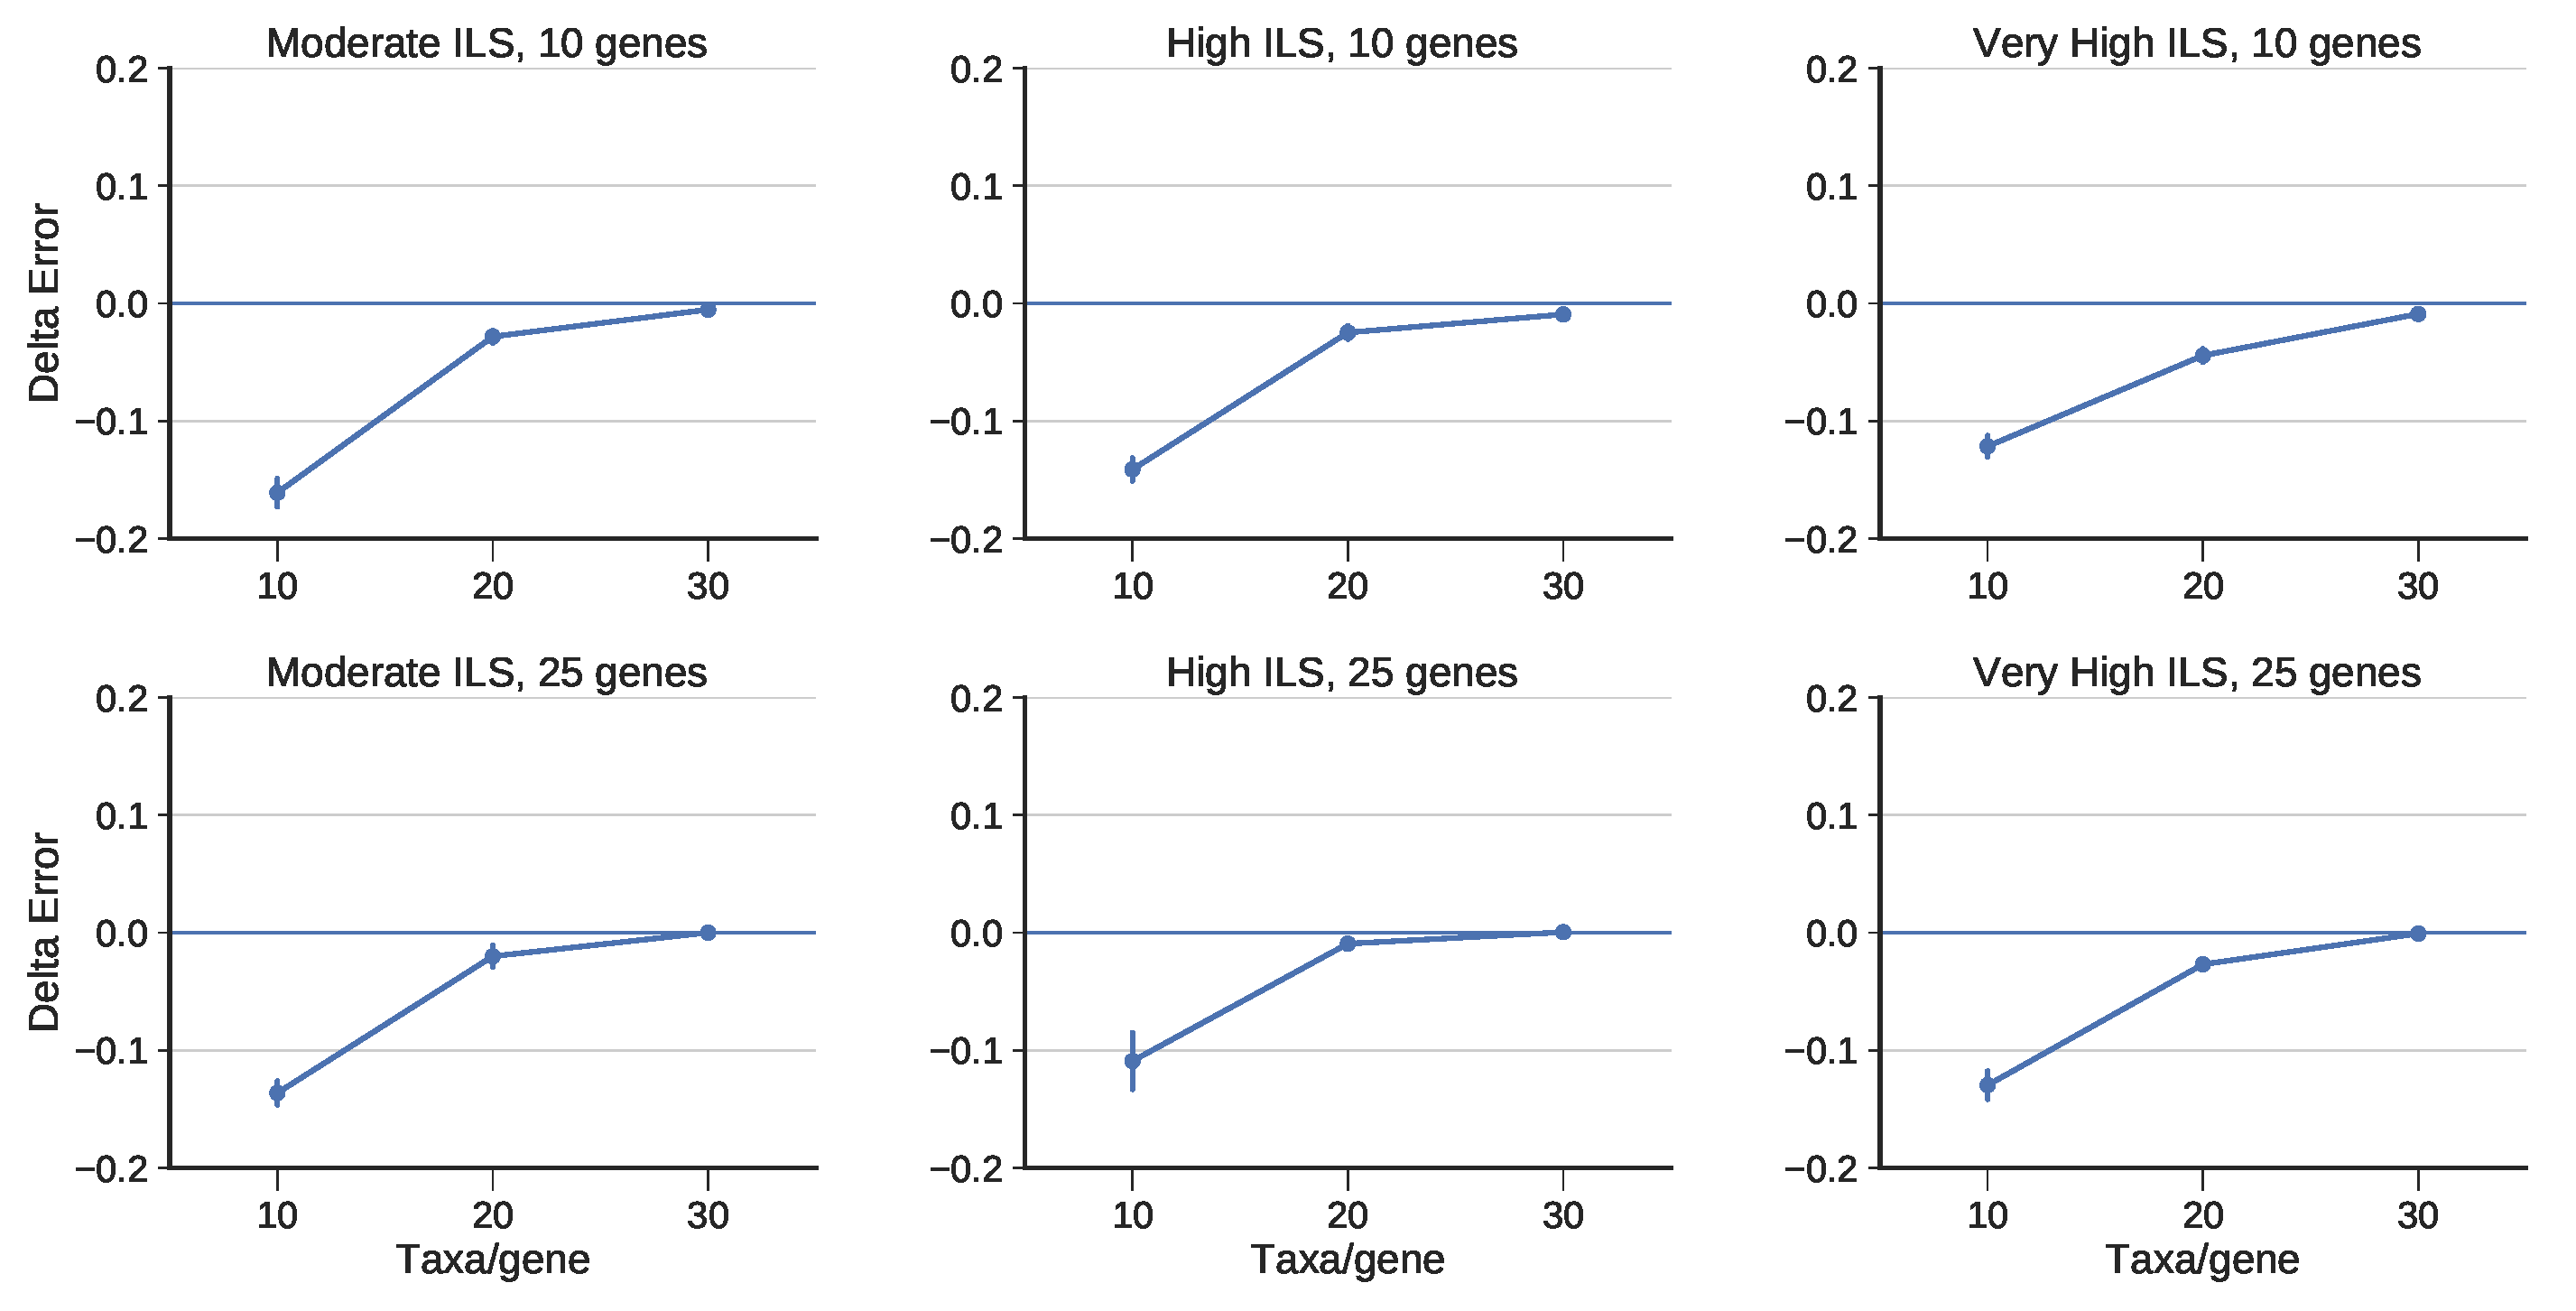
\includegraphics[width=.9\textwidth]{siesta-figs/astral_missing_delta_error}
  \caption[Change in topological error between ASTRAL and the SIESTA strict consensus of ASTRAL trees on simulated data, varying ILS level and number of genes]{
We show Delta-error (change in mean topological error between a single ASTRAL tree and the strict consensus of  the set of ASTRAL trees) on simulated phylogenomic datasets with three different ILS levels, 50 species,  and 25 incomplete estimated gene trees; values below 0 indicate that the strict consensus of the ASTRAL trees is more accurate  than a single ASTRAL tree.
 We show results for 25 replicates.
Error bars indicate the standard error; 
  topological error is the average of the FN and FP error rates.
  }
    \label{siesta::fig:astral-error}
\end{figure}

\begin{figure}[ht]
  \centering
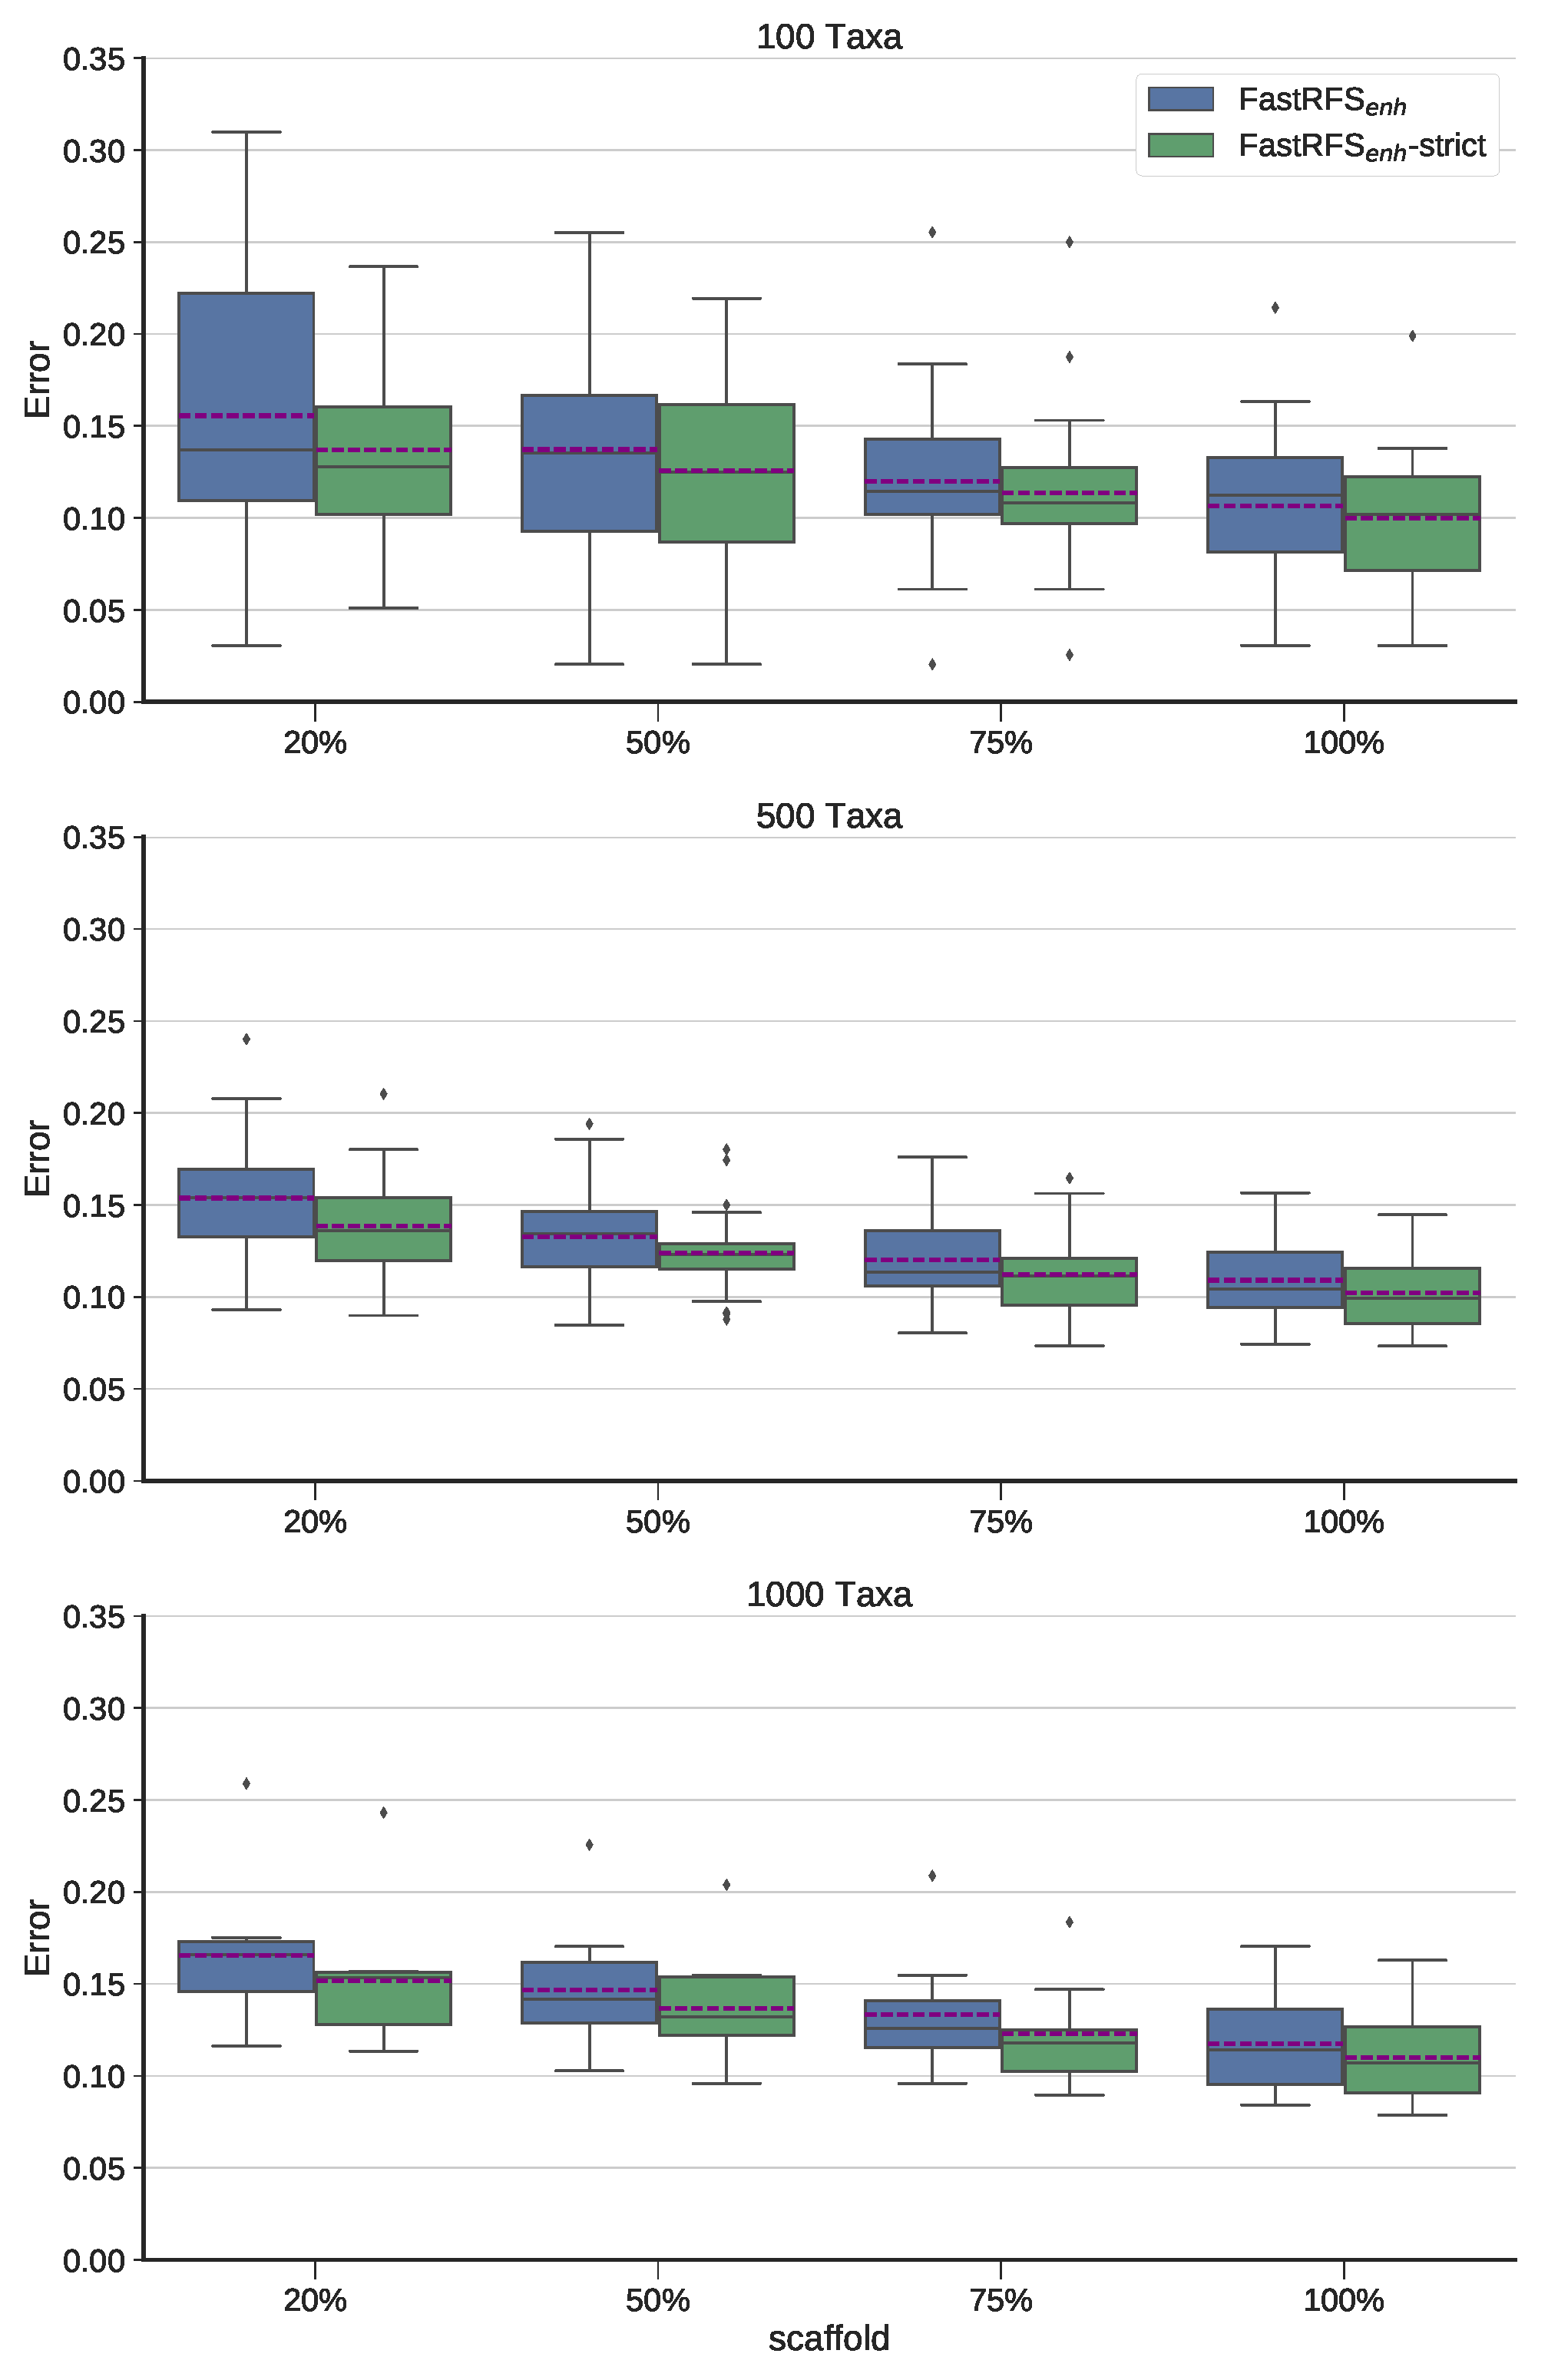
\includegraphics[width=\textwidth, height=0.8\textheight,keepaspectratio]{siesta-figs/fastrfs-enh-siesta-comparison}
\caption[Error rates for FastRFS$_{enh}$ and FastRFS$_{enh}$+SIESTA (strict consensus) on simulated datasets]{We compare a single FastRFS$_{enh}$ supertree to FastRFS$_{enh}$+SIESTA (the strict consensus of the optimal FastRFS$_{enh}$ supertrees) on unrooted supertree datasets.
Error shown is the normalized average topological error (i.e., average of FN and FP rates) between true and estimated supertrees.
Error bars indicate the standard error. 
There are 25 replicates each for the 100- and 500-taxon datasets, and 10 replicates for the 1000-taxon datasets.
   }
     \label{siesta::fig:supertree-error-unrooted}
\end{figure}


For rooted supertree datasets, we explore another supertree method called
 the Bad Clade Deletion (BCD) supertree method, which can only be used with rooted source trees.
 As shown in \cite{fleischauer2017bad}, BCD produced more accurate species trees (with respect to the F1 metric) than FastRFS$_{basic}$ and several other supertree methods.
 We confirm that BCD outperforms FastRFS$_{basic}$ with respect to the F1 metric (Additional file 1, Fig.~S4),  and also note that BCD outperforms FastRFS$_{basic}$ with respect to
the RF error rate   (Additional file 1, Fig.~S5).  
However, it is not known whether BCD is more accurate than FastRFS$_{enh}$ or FastRFS$_{BCD}$, nor whether using SIESTA enables some FastRFS variant  to outperform BCD. 
We compared these three methods with respect to RF errors (Additional file 1, Fig.~S6) and F1 scores (Additional file 1, Fig.~S7). 
The two FastRFS variants are very close in accuracy with respect to both criteria, with a slight advantage to FastRFS$_{BCD}$. 
Interestingly, the comparison to BCD shows that the FastRFS variants are less accurate on the sparse scaffolds than BCD, but slightly more accurate on the 100\%-scaffold.
Overall, therefore, FastRFS$_{BCD}$ has a slight advantage over the other FastRFS variants on these rooted supertree datasets, and is competitive with BCD (worse under some conditions
and better under others). 



\begin{figure}[ht]
  \centering
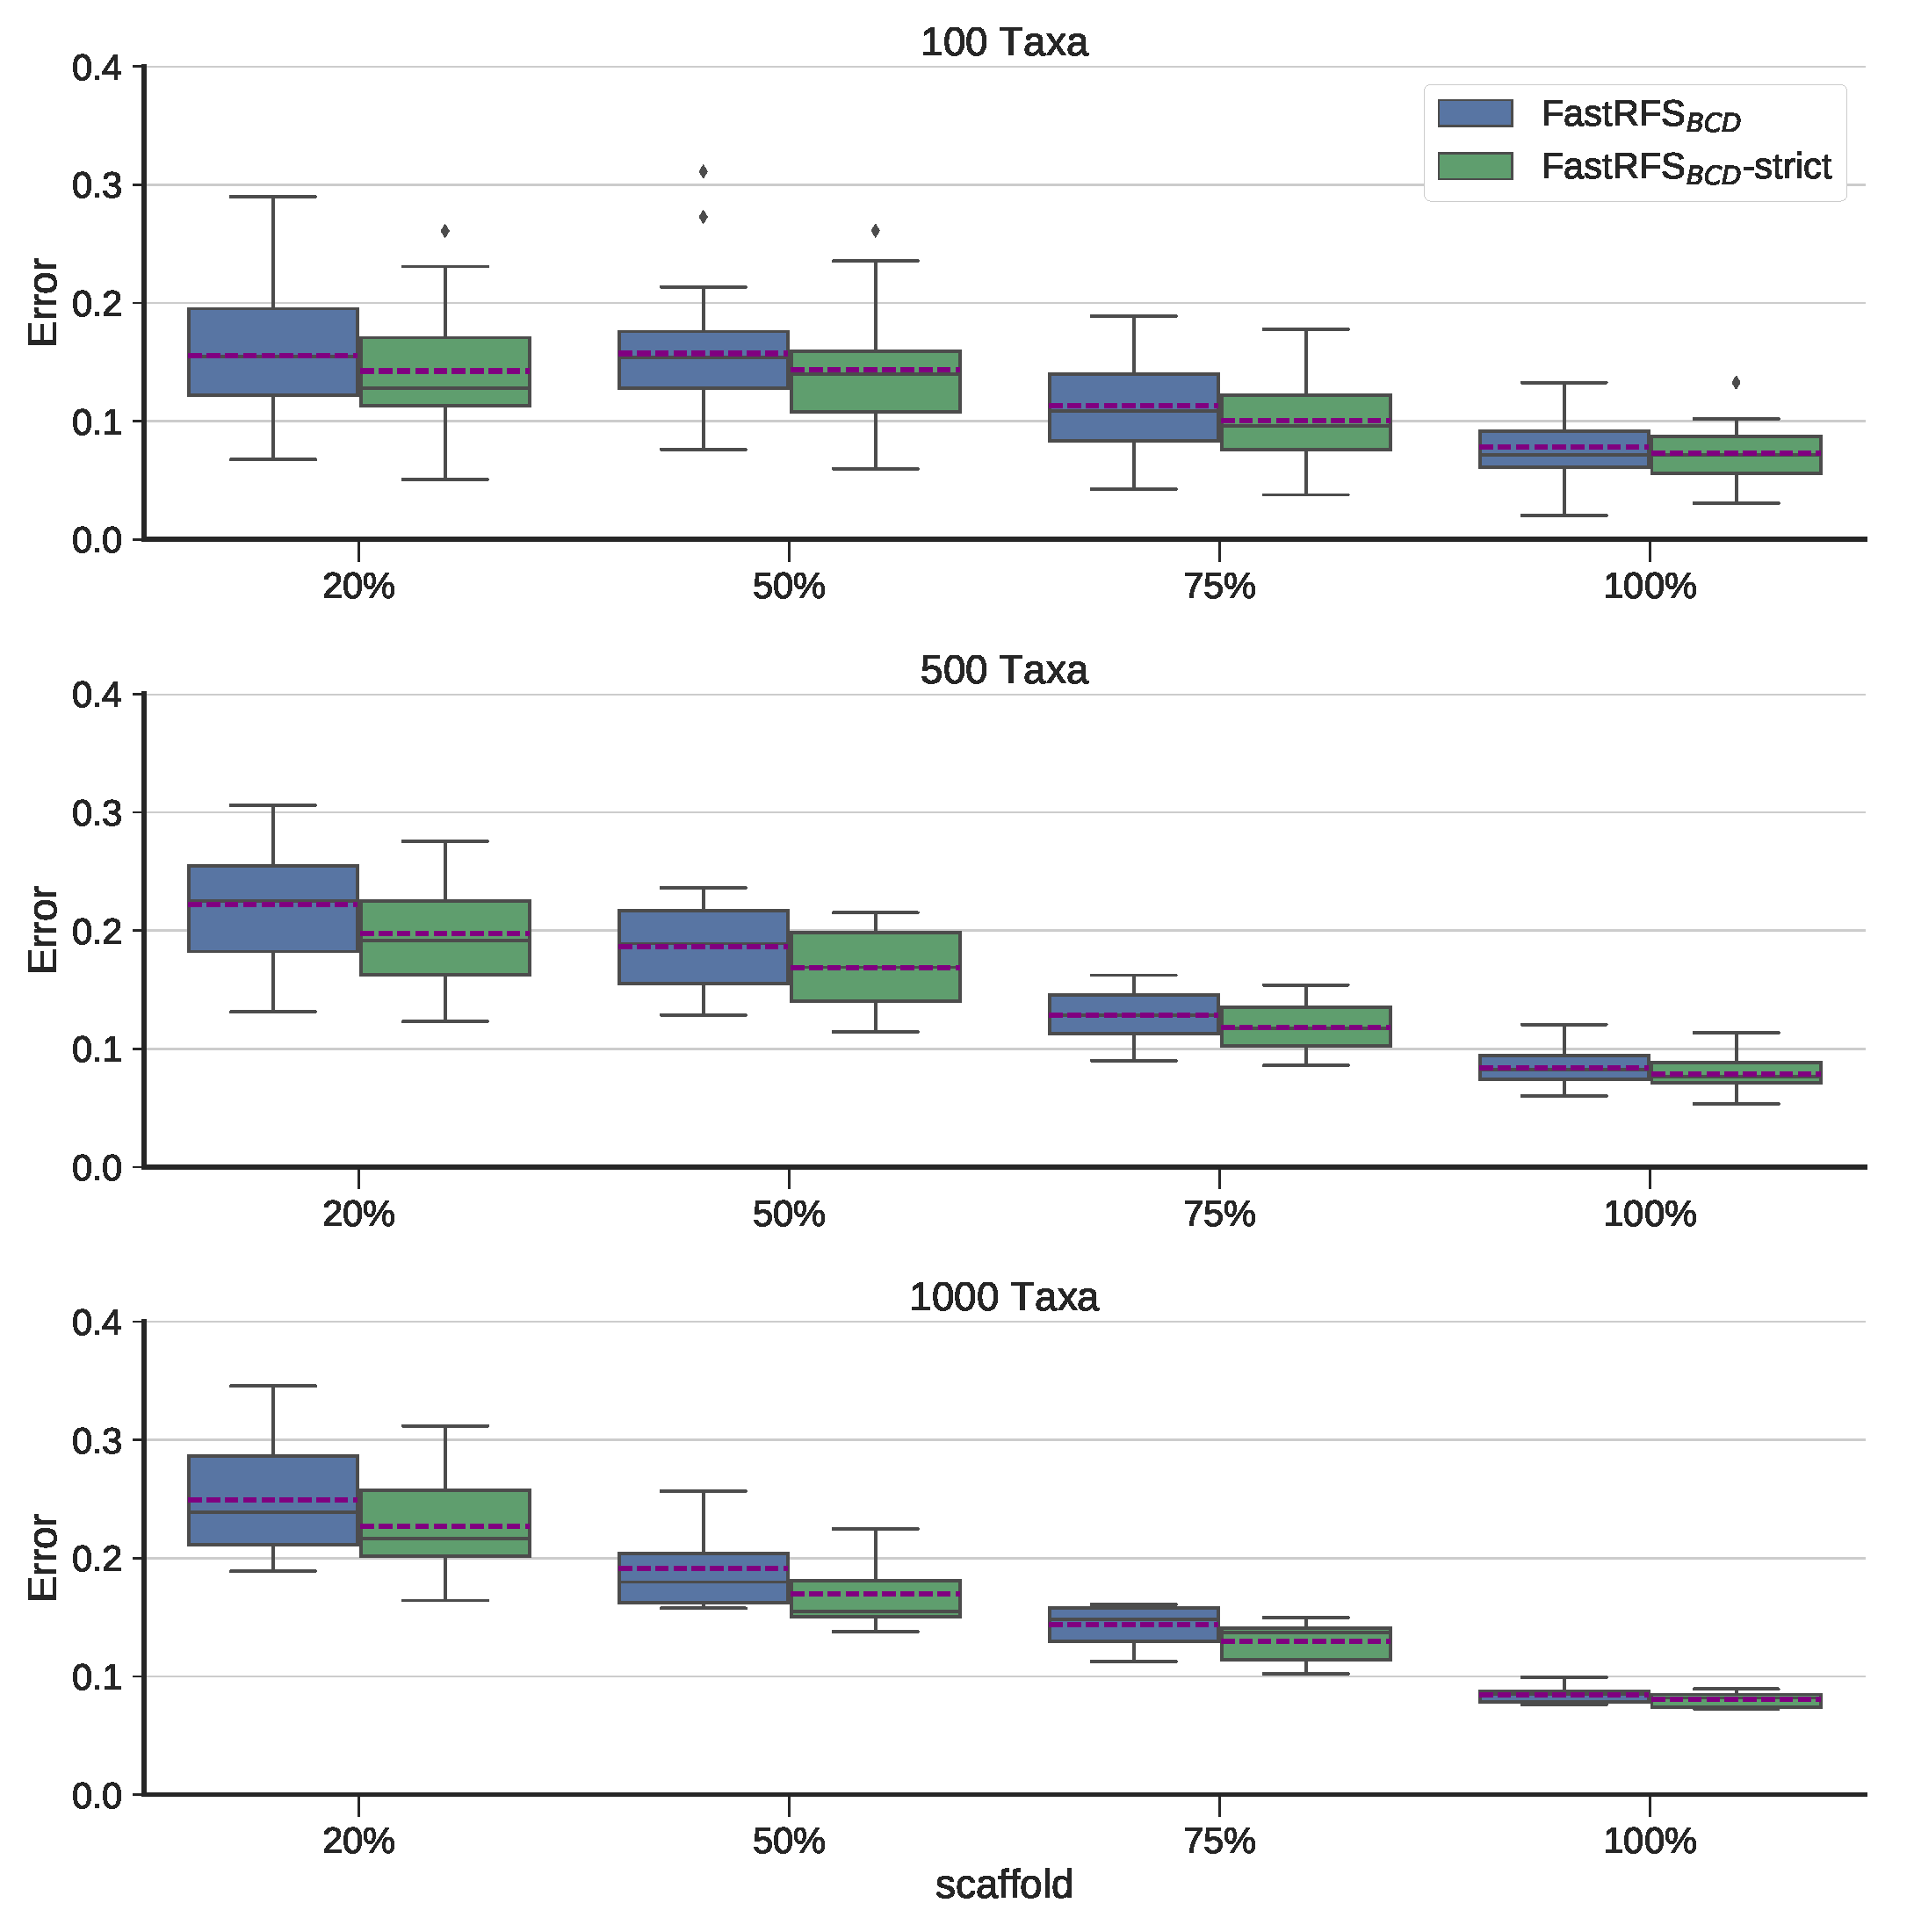
\includegraphics[width=1\textwidth]{siesta-figs/fastrfs-bcd-siesta-comparison}
\caption[Error rates for FastRFS$_{BCD}$ and FastRFS$_{BCD}$+SIESTA (strict consensus) on simulated datasets]{We compare a single FastRFS$_{BCD}$ supertree (FastRFS$_{BCD}$) to FastRFS$_{BCD}$+SIESTA (the strict consensus of the optimal FastRFS$_{BCD}$ supertrees)  on rooted supertree datasets.
Error shown is the normalized average topological error (i.e., average of FN and FP rates) between true and estimated supertrees.
Error bars indicate the standard error. 
There are 25 replicates each for the 100- and 500-taxon datasets, and 10 replicates for the 1000-taxon datasets.
  }
     \label{siesta::fig:supertree-error-rooted}
\end{figure}




\begin{figure}[ht]
  \centering
 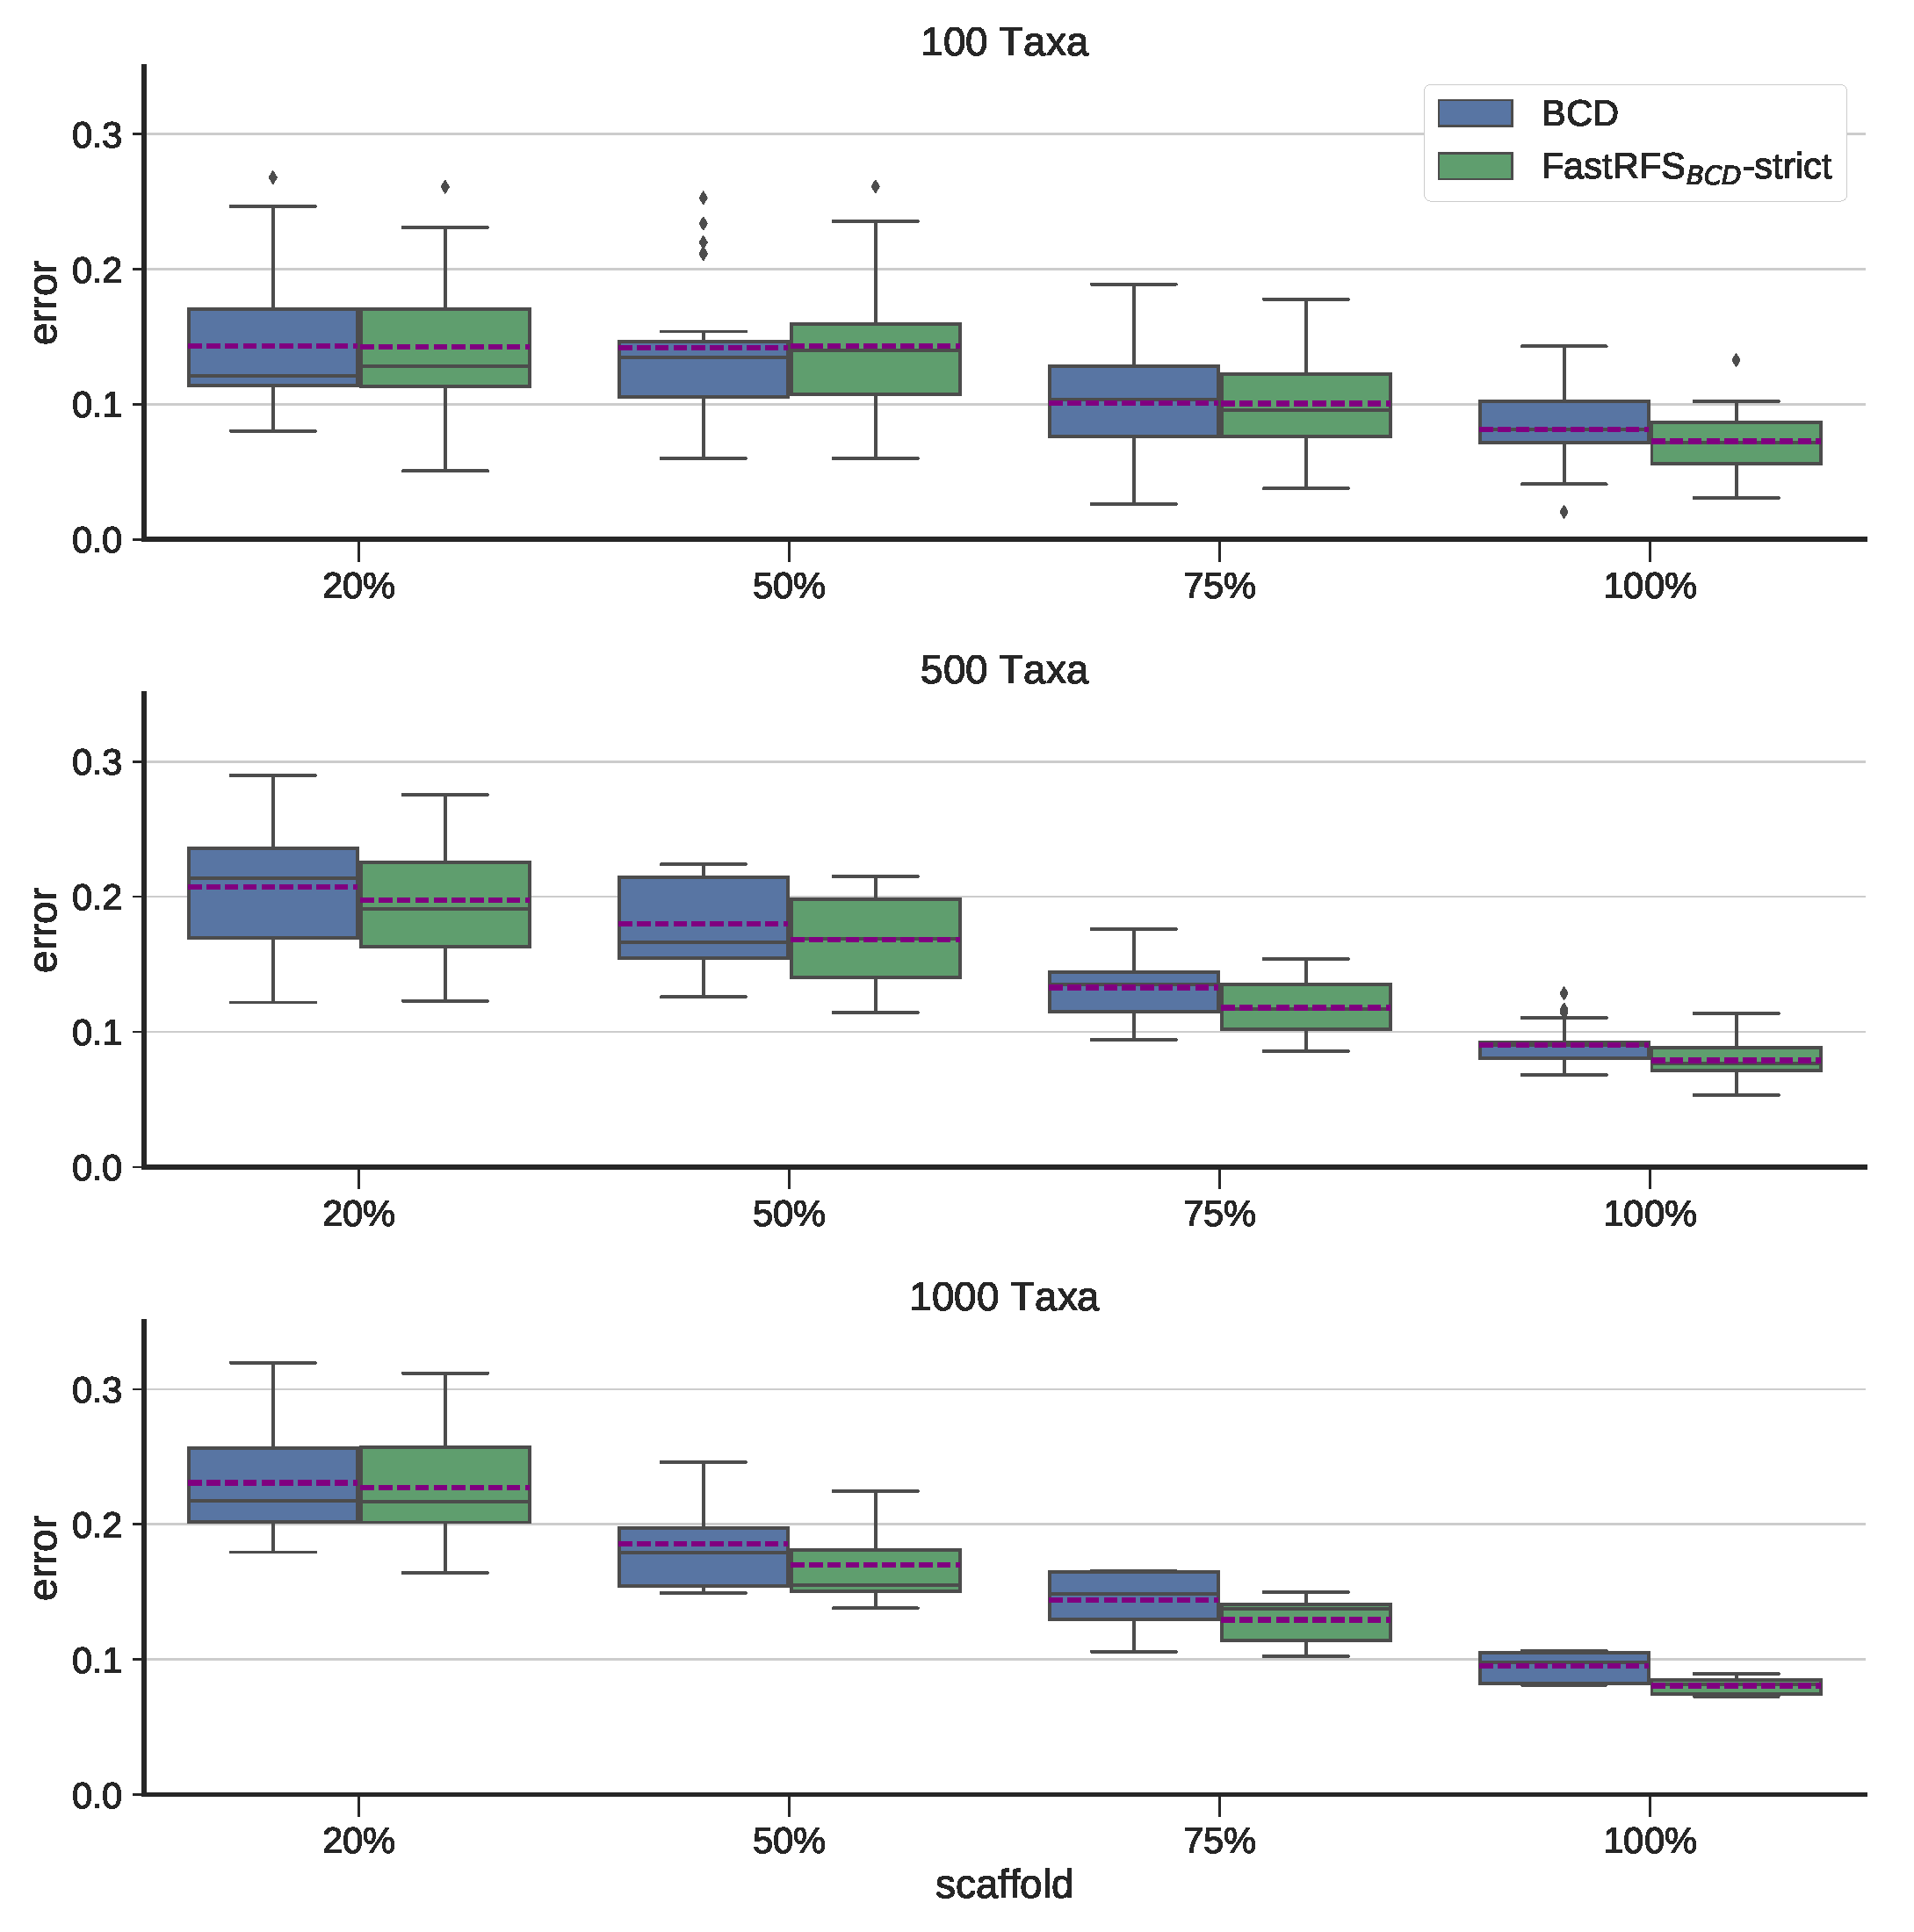
\includegraphics[width=1\textwidth]{siesta-figs/best-supertree-comparison-mult_only}
\caption[Error rates for BCD and FastRFS$_{BCD}$+SIESTA (strict consensus) on simulated datasets]{We compare Bad Clade Deletion (BCD) supertrees to the strict consensus of FastRFS$_{BCD}$ supertrees on rooted supertree datasets.
Error shown is the normalized average topological error (i.e., average of FN and FP rates) between true and estimated supertrees.
Error bars indicate the standard error. 
There are 25 replicates each for the 100- and 500-taxon datasets, and 10 replicates for the 1000-taxon datasets.
  }\label{siesta::fig:supertree-bcd-error}
\end{figure}


We then examined whether computing the strict consensus improves FastRFS$_{BCD}$ enough to enable it to outperform BCD.
We first observed that
 the strict consensus of the FastRFS$_{BCD}$ supertrees was more accurate than a single FastRFS$_{BCD}$ supertree (Fig.~\ref{siesta::fig:supertree-error-rooted}).
Furthermore, using SIESTA to compute the strict consensus of the optimal trees found by   FastRFS$_{BCD}$ produces supertrees that are generally (but not always) more accurate than BCD 
(Fig. \ref{siesta::fig:supertree-bcd-error} shows average tree error  and  Additional file 1, Fig.~S8 shows the F1 scores).
The differences are smallest on the 100-taxon datasets, but the strict consensus of the FastRFS$_{BCD}$ trees is generally more
accurate than BCD on the larger datasets, especially for the denser scaffolds.  
Thus,  the use of SIESTA enables FastRFS$_{BCD}$ to outperform BCD.

















\subsection{Experiment 4: ASTRAL+SIESTA vs.~ASTRAL on simulated phylogenomic data}


% \begin{figure}[ht]
%   \centering
%  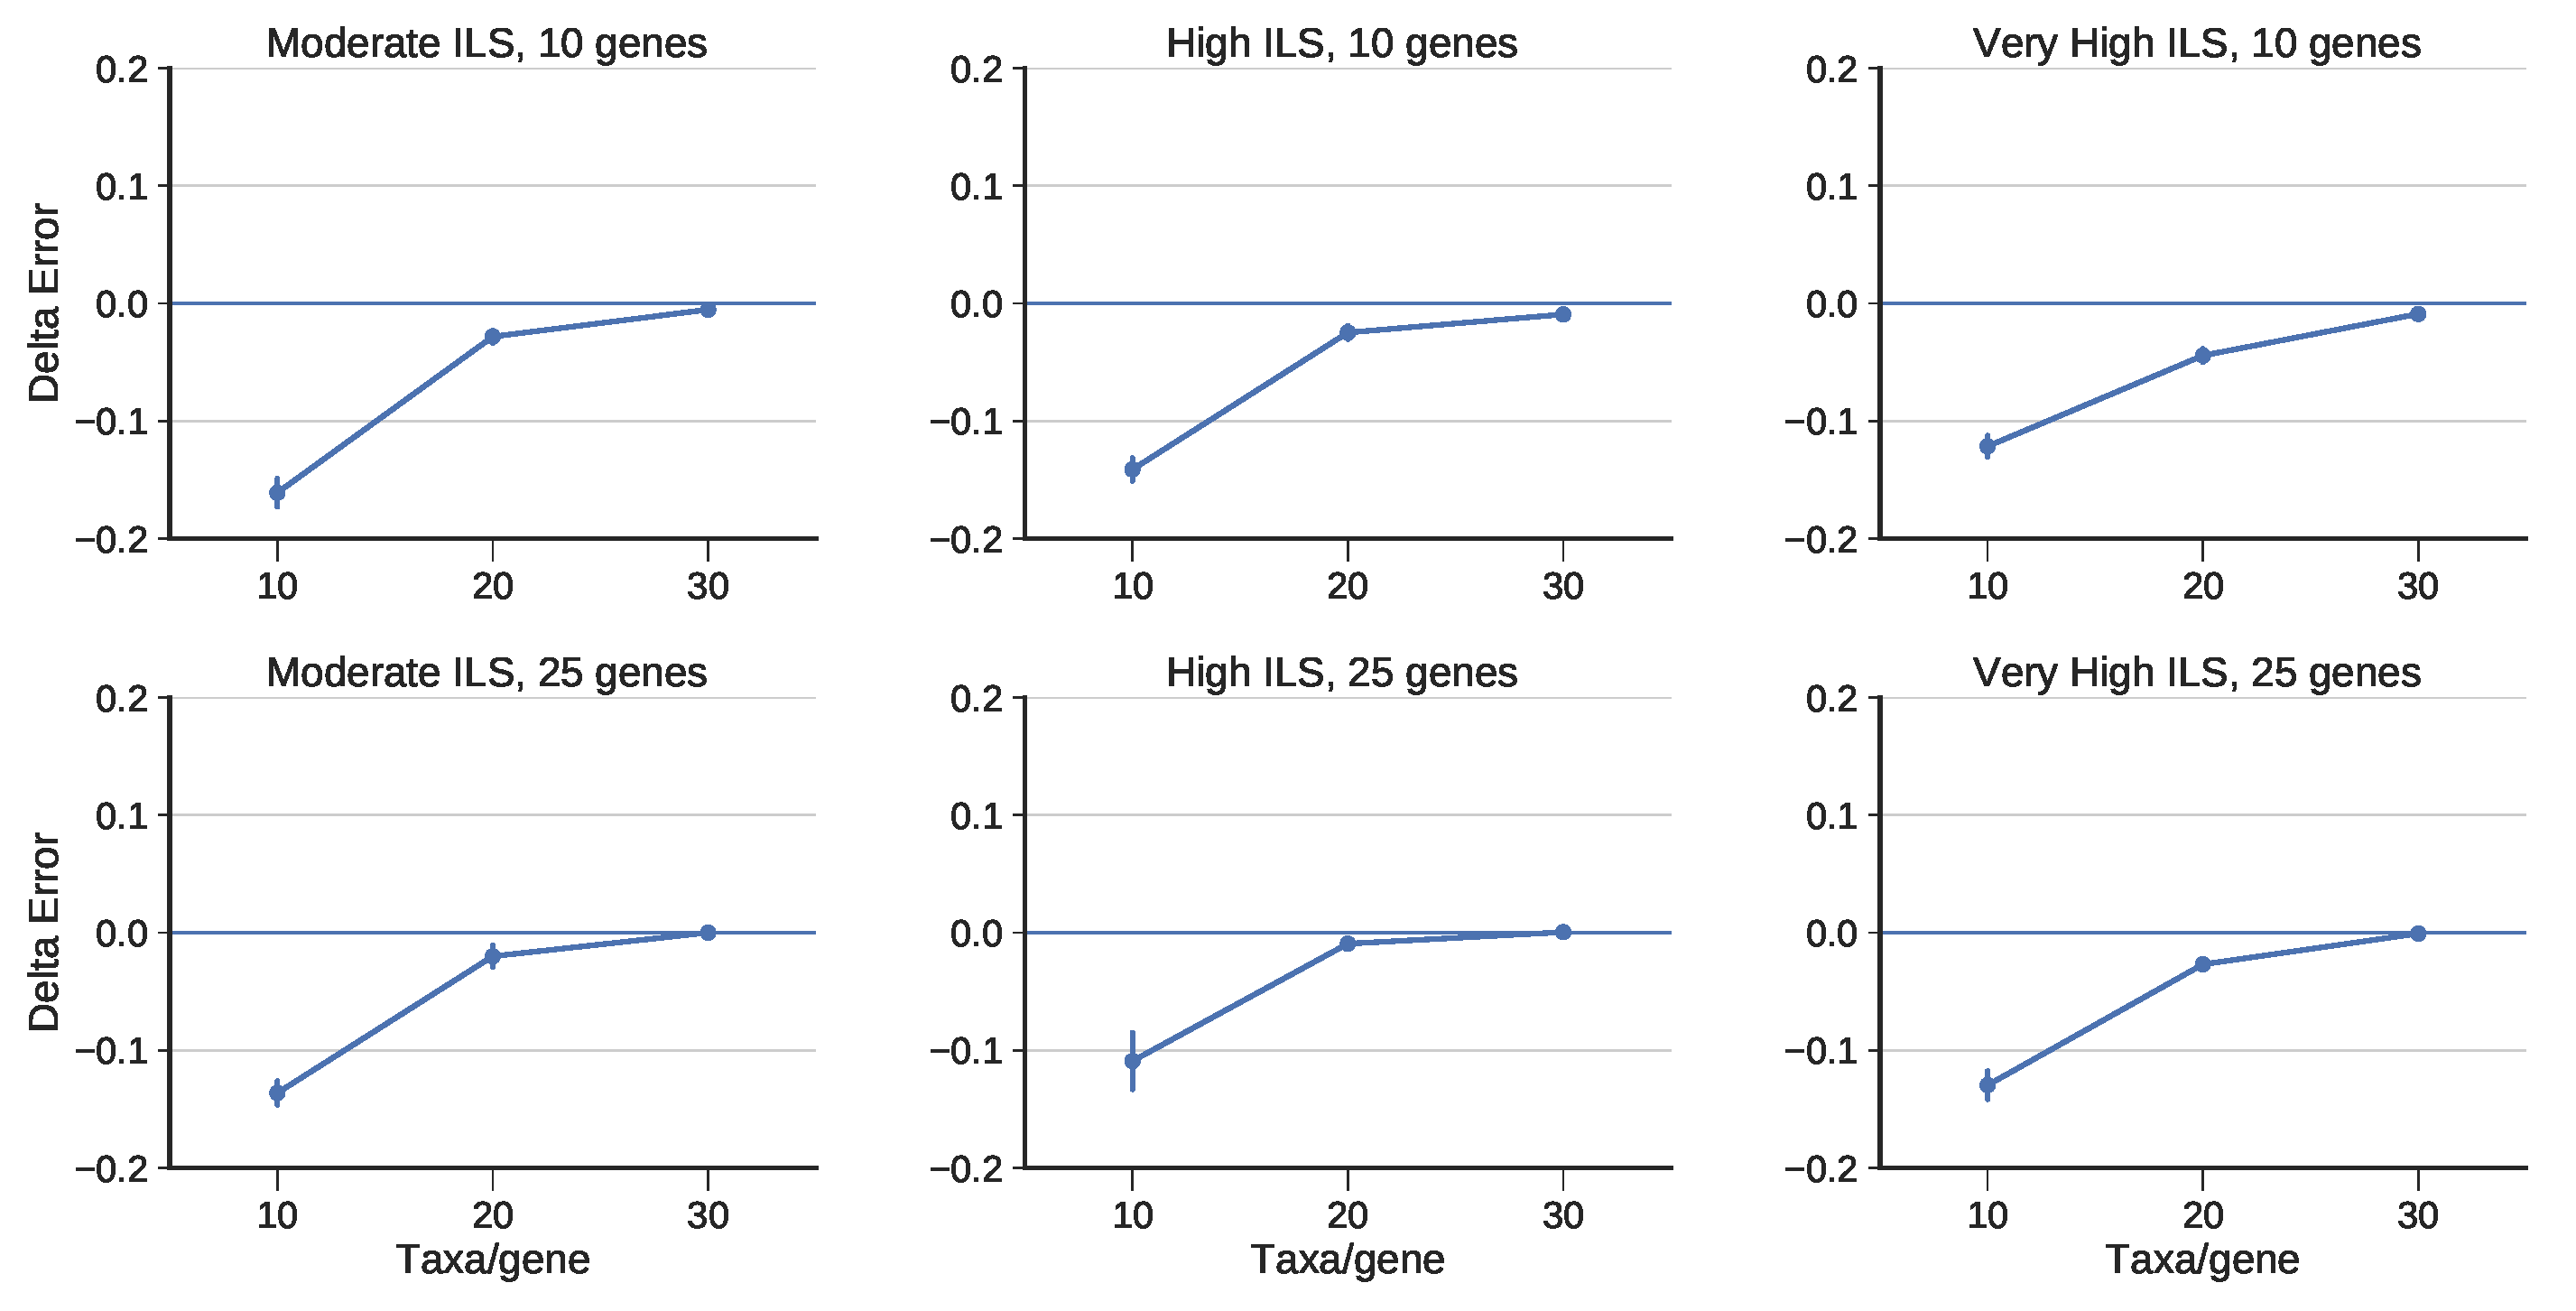
\includegraphics[width=.9\textwidth]{siesta-figs/astral_missing_delta_error}
%   \caption[Change in topological error between ASTRAL and the SIESTA strict consensus of ASTRAL trees on simulated data, varying ILS level and number of genes]{
% We show Delta-error (change in mean topological error between a single ASTRAL tree and the strict consensus of  the set of ASTRAL trees) on simulated phylogenomic datasets with three different ILS levels, 50 species,  and 25 incomplete estimated gene trees; values below 0 indicate that the strict consensus of the ASTRAL trees is more accurate  than a single ASTRAL tree.
%  We show results for 25 replicates.
% Error bars indicate the standard error; 
%   topological error is the average of the FN and FP error rates.
%   }
%     \label{siesta::fig:astral-error}
% \end{figure}



\begin{figure}[ht]
  \centering
 \includegraphics[width=.9\textwidth]{siesta-figs/astral-missing-ntrees}
    \caption[Change in topological error between ASTRAL and the SIESTA strict consensus of ASTRAL trees on simulated data, varying amount of missing data]{
We show the FN and FP error rates of the strict consensus of  ASTRAL trees, compared to a single ASTRAL tree,  on simulated phylogenomic datasets with 50 species and 25 incomplete estimated gene trees; values below 0 indicate that the strict consensus ASTRAL is more accurate for that criterion  (i.e., it has lower error) than ASTRAL. The x-axis shows the number of optimal trees, and 
 we show results for 25 replicates.
Error bars indicate the standard error.
  }
  \label{siesta::fig:astral-error-vs-number}
\end{figure}

As noted earlier, ASTRAL often returns only one optimal tree, so that the strict consensus of the optimal ASTRAL trees cannot differ from the single best tree. 
In this experiment, we restrict the attention to the datasets on which ASTRAL found more than one tree.
In general, this occurred for the phylogenomic datasets with substantial levels of missing data (i.e., when we deleted species randomly from genes). 
For these cases, we see that the average topological error rates  for the strict consensus of the ASTRAL trees  are lower than the error rate for a single ASTRAL tree (Fig.~\ref{siesta::fig:astral-error}) under three different ILS levels, when there is missing data. However, the degree to which the strict consensus of the ASTRAL  trees improves over a single ASTRAL depends upon the amount of missing data.

A more nuanced analysis is shown in  Figure \ref{siesta::fig:astral-error-vs-number}, where we explore how
the number of optimal trees impacts the FN and FP rates for the strict consensus.
Note that the FN rate of the strict consensus is very similar to the FN rate of a single optimal ASTRAL tree, but the strict consensus has a much lower FP rate;
hence the  strict consensus has a reduced  average  error rate compared to a single best tree.
Although  the FN rates are slightly higher under lower ILS conditions, the FP rates drop more than the  FN rates increase, so that the same overall trends are  similar  (Additional file 1, Fig.~S9). %correct figure number
 



\subsection{Experiment 5: Results on biological datasets}



For the biological datasets,  we do not know the true species tree (which is the unstated objective of the supertree analysis), and so we cannot evaluate accuracy. 
However, we show how to use SIESTA to provide meaningful branch support in estimated species trees.



\begin{figure}[ht]
  \centering
  \includegraphics[width=0.9\textwidth]{siesta-figs/bio_fastrfs_enh_supports.png} 
  \caption[Histogram of support values for edges in the FastRFS$_{enh}$ greedy consensus tree on the unrooted supertree datasets.]{Histogram of support values for edges in the FastRFS$_{enh}$ greedy consensus tree on the unrooted supertree datasets. These support values are
    the percentages of the optimal trees they appear in. 
    Although the majority of the edges have 100\% support in each tree, some edges have low support, suggesting that they are not as reliable as the higher support edges.}
     \label{siesta::fig:support_fastrfs}
\end{figure}

\paragraph{Biological supertree datasets. }
We use SIESTA to compute the greedy consensus tree of the FastRFS$_{enh}$ supertrees on the unrooted supertree datasets, and then annotated each edge in the greedy consensus supertree with the fraction of the optimal trees  on the dataset.
Figure \ref{siesta::fig:support_fastrfs} shows that most of the edges in the greedy consensus of the optimal FastRFS$_{enh}$ supertrees for each of these datasets have 100\% support, indicating that these edges are consistent across all optimal trees.
It also shows that some  edges are only found in about half (sometimes even less) of the optimal trees, and so should not be considered as reliable.
However, this depends on the dataset:  nearly all the edges in the greedy consensus of the optimal FastRFS$_{enh}$ supertrees for the placental mammals dataset have 100\% support, while the THPL and CPL datasets have a substantial fraction of edges that appear in at most 60\% of the optimal FastRFS$_{enh}$ supertrees.

  
\paragraph{Hymenoptera phylogenomic dataset. }

\begin{figure}[!ht]

\includegraphics[width=0.8\textwidth]{siesta-figs/hymenoptera}
\caption[Four optimal ASTRAL trees on biological Hymenoptera dataset]{The four optimal ASTRAL trees on the Hymenoptera dataset, each rooted at the outgroup, and given with local posterior probabilities for branch support. The four trees differ only in two groups: (1) Solenopsi, Apis, and Vesputal\_C, and (2) Acyrthosi, Myzus, and Acyrthosp. }\label{siesta::fig:hymenoptera-optimal}
\end{figure}

\begin{figure}[!ht]
\centering
\includegraphics[width=0.9\textwidth]{siesta-figs/hymenoptera-figure8.pdf}
\caption[ASTRAL Maximum Clade Credibility Tree and strict consensus tree on biological Hymenoptera dataset]{The ASTRAL  Maximum Clade Credibility (MCC) tree (left) with branch support and the strict consensus tree (right) on the Hymenoptera dataset. 
The ASTRAL MCC tree is topologically identical to one of the four ASTRAL trees, but has different branch support; in particular, the branch support on the clades in question is half the branch support in the original ASTRAL trees on these clades. 
The ASTRAL strict consensus tree makes these two clades into polytomies. 
}\label{siesta::fig:hymenoptera-fig8}
\end{figure}


The Hymenoptera dataset is a phylogenomic dataset with 21 taxa and 24 genes.
There are four optimal ASTRAL trees on this dataset (shown in Fig.~\ref{siesta::fig:hymenoptera-optimal}). 
The differences between these four trees are restricted to two clades with three species each: (1) Solenopsi, Apis, and Vesputal\_C, and (2) Acyrthosi, Myzus, and Acyrthosp. 
The strict and majority consensus trees (Fig.~\ref{siesta::fig:hymenoptera-fig8}) on these four ASTRAL trees are identical, and present these two groups as completely unresolved.
The MCC tree (Fig.~\ref{siesta::fig:hymenoptera-fig8}) on this set of four ASTRAL trees matches one of the four trees with respect to topology, but has different branch support on the edges, so that the branch support for the two clades in question are halved in comparison to the four ASTRAL trees; thus, the MCC tree appropriately identifies these clades as having very low support.


\paragraph{Sigmontidine rodent  phylogenomic dataset. }
The Sigmontidine rodent dataset is a phylogenomics dataset with 285 taxa and 11 genes, and there are 72 optimal ASTRAL trees on this dataset. 
The species tree computed on this dataset in \cite{maestri2017ecology} was a concatenated Bayesian tree using MrBayes \cite{ronquist2012mrbayes}, with branch support based on posterior probabilities. The Sigmontidine rodent dataset had 72 optimal ASTRAL trees. 
We computed the ASTRAL MCC tree, and then collapsed all branches with support less than   $75\%$; this produced a tree with only 74 internal edges.  This dataset has 285 taxa, meaning that a fully resolved tree would have 282 internal branches.  By comparison, the MrBayes tree has 223 internal branches after collapsing branches with less than $75\%$ support. 

Comparing the MrBayes tree with the ASTRAL MCC tree, we find that 64 bipartitions are present and highly supported in both trees.  After collapsing the edges with lower support, we are left with only the high support edges. Six  highly supported bipartitions are present in the ASTRAL MCC tree and compatible with the collapsed MrBayes tree, and  three bipartitions are present in the ASTRAL MCC tree and incompatible with the collapsed MrBayes tree.  153 highly supported bipartitions are present in the MrBayes tree and compatible with (but not present in) the collapsed ASTRAL MCC tree, and 5 highly supported bipartitions in the MrBayes tree are incompatible with the collapsed ASTRAL MCC tree.  The highly supported conflicts between the trees occur in three locations:
\begin{enumerate}
\item The MrBayes tree has \emph{Akodon Mimus} as the root of the \emph{Akodon} genus, while the ASTRAL MCC tree has it internal to \emph{Akodon} (the root of \emph{Akodon} is not resolved with greater than 75\% support). 
\item The MrBayes tree and the ASTRAL MCC tree swap the locations of the \emph{Holochilus} and \emph{Sooretamys} clades, with ASTRAL putting \emph{Holochilus} as the basal clade and  MrBayes  putting \emph{Sooretamys} as the basal clade. 
\item The ASTRAL MCC tree and the MrBayes tree disagree about some resolutions within the \emph{Oligoryzomys} clade. 
\end{enumerate}
These placements are in general not well established in the literature \cite{alvarado2013new,gonzalez2014molecular,machado2014phylogeny}, and so it is not clear which of the two trees is more likely to be correct for these questions.


The difference between a single ASTRAL tree and the ASTRAL MCC tree  is therefore quite significant for some datasets. To understand these differences, recall that  the support values are obtained using posterior probabilities based on quartet trees around an edge in a single optimal tree. 
However, a simple example can explain why this can be misleading. Suppose $T_1$ and $T_2$ are the only trees that are optimal for ASTRAL, and that $T_1$ has a split $\pi$ that $T_2$ does not have.
Then under the assumption that $T_1$ and $T_2$ are both equally likely to be the true species tree, the {\em maximum} probability that $\pi$ can be a true split is $0.5$ -- since it is in only one optimal tree.  
It is easy to see that any support value greater than $0.5$ produced when $T_1$ is examined is inflated, and that a correction must be made that takes into consideration that $T_2$ is also an optimal tree.
SIESTA's way of calculating support explicitly enables this correction, since it explicitly considers the support of each bipartition obtained from the entire set of optimal trees. 


\begin{table}[!ht]
\centering
\begin{tabular}{|c|c|c|c|}
\hline
Scaffold factor & FastRFS$_{basic}$ (single)  & FastRFS$_{basic}$ (strict consensus)& Difference\\
\hline
\hline
 20\%  &$31.6$       &$31.6$ & $<$ 0.1\\
50\% &$39.3$       &$39.4$ & 0.1\\ 
75\% &$37.5$       &$37.8$ & 0.3 \\
100\% &$34.6$       &$34.6$ & $<$ 0.1\\
\hline
\end{tabular}

\caption[Comparison of running times for FastRFS$_{basic}$ with and without SIESTA]{Running time (in seconds, rounded to the nearest tenth) on the 1000-taxon rooted supertree datasets for FastRFS$_{basic}$ and for the computation of the strict consensus of the
FastRFS$_{basic}$ optimal trees (averaged over 10 replicates).  The difference in running time to compute the strict consensus of the set of optimal trees compared to computing a single best tree is at most $0.3$ seconds. }
\label{siesta::table:runningtime-FastRFS$_{basic}$}
\end{table}

\begin{table}[!ht]
\centering
\begin{tabular}{|c|c|c|c|c|c|}
\hline
 Scaffold factor & BCD & FastRFS$_{BCD}$ (single)  & FastRFS$_{BCD}$ (strict consensus)& Difference\\
\hline
\hline 
20\% &$10.2$       &$33.1$       &$33.5$ & 0.4 \\
50\%  &$8.1$        &$41.8$       &$42.3$ & 0.5 \\ 
75\% &$9.2$        &$39.9$       &$40.1$ &0.2 \\
100\% &$14.4$       &$36.3$       &$36.4$ &  0.1\\
\hline
\end{tabular}
\caption[Running times for BCD and for FastRFS$_{BCD}$ with and without SIESTA]{Running time (in seconds) on the 1000-taxon rooted supertree datasets for  BCD, FastRFS$_{BCD}$, and for the computation of the strict consensus of the
FastRFS$_{BCD}$ optimal trees (averaged over 10 replicates). The difference in running time to compute the strict consensus of the set of optimal trees compared to computing a single best tree is at most half a second.}

\label{siesta::table:runningtime-fastrfs-bcd}
\end{table}


\subsection{Experiment 6: Running Time}
We explore the  computational impact of using SIESTA  to compute the strict consensus of the optimal trees found using two variants of FastRFS  on the rooted supertree datasets with 1000 species.
We compare the cost of using FastRFS$_{basic}$ to find a single tree to the total running time needed
to compute the strict consensus of the FastRFS$_{basic}$ supertrees (Table \ref{siesta::table:runningtime-FastRFS$_{basic}$}).
All methods complete in under a minute (actually under 40 seconds), and that the difference in terms of time needed to compute a single FastRFS$_{basic}$ tree and the strict consensus of all the optimal FastRFS$_{basic}$ trees
is at most $0.3$ seconds.
We  also compare the time needed to run BCD, FastRFS$_{BCD}$, and the total time needed to compute the
strict consensus of the FastRFS$_{BCD}$ supertrees (Table \ref{siesta::table:runningtime-fastrfs-bcd}).
Note that BCD is substantially faster than FastRFS$_{BCD}$, but that all methods complete in less than a minute.
Note also that the difference in terms of time needed to compute a single FastRFS$_{BCD}$ tree and the strict consensus of all the optimal FastRFS$_{BCD}$ trees
is at most $0.5$ seconds 

Thus, the additional time needed to compute the strict consensus of the set of optimal trees is less than half a second. This is particularly noteworthy, given the number of optimal trees that are found by FastRFS$_{basic}$ on these 1000-taxon supertree datasets. Overall, these data show that the cost of using SIESTA is small, and represents a small percentage of the total time needed to find a single tree.


\section{Conclusions}



SIESTA is a simple technique for computing a data structure that implicitly represents a set of optimal trees found during the dynamic programming algorithms used by ASTRAL and FastRFS, but  SIESTA is generalizable to any algorithm that uses the same basic dynamic programming structure. 
Once the data structure is computed, it can be used in multiple ways to explore the solution space. 
In particular, it can be used to count the number of optimal solutions and determine the support for a particular bipartition, thus enabling the estimation of the support on branches for a given optimal tree that takes into account the existence of  other optimal trees.

We studied SIESTA in conjunction with ASTRAL and FastRFS on a collection of biological and simulated datasets. This study showed that using SIESTA to compute the strict consensus produced a benefit for some methods in some cases, but not in all.
The trends we observed clearly indicate that when there are many optimal trees, the use of the strict consensus tree results in a substantial reduction in the false positive rate and a lesser increase in the false negative rate, for an overall reduction in topological error. 
Conversely, when there are only a small number of optimal trees, there is little change between the strict consensus tree and any single optimal tree.
Thus, the impact of using the strict consensus depends on the number of optimal solutions, which tended to be larger for all FastRFS variants than for ASTRAL.
We also saw that the number of optimal trees for ASTRAL depends on the amount of missing data, so that the benefit of using SIESTA with ASTRAL to compute the strict consensus seems to be reliable only when there is missing data. 
The study also showed that  FastRFS typically benefited from using the strict consensus tree, while ASTRAL's benefit varied with the dataset, as a result of the differences in numbers of optimal trees.


Our study showed that using SIESTA to produce a maximum clade credibility (MCC) tree with ASTRAL provided a  more statistically meaningful point estimate of the true species tree than any single optimal ASTRAL tree, especially with respect to appropriately modified branch support values that take the multiple optima into account.
Thus, SIESTA provides multiple benefits to species tree and supertree estimation: identifying cases where there is a unique optimum and providing better point estimates of the true tree when there are multiple optima.

Finally, there are many other methods  that also use a dynamic programming approach for tree estimation (often within a constrained search space), and SIESTA can be used with these methods in similar ways. Future work should explore the impact of SIESTA with these other methods. 



\section{Supplementary Data for SIESTA}

\subsection{Software Commands and Version Numbers}
We provide the detailed commands for the various analyses we performed.
\begin{itemize}
\item

RAxML v8.2.6 was used to estimate gene trees on the phylogenomic simulated data with arguments ``-m GTRGAMMA -p 12345 -n  $<$jobname$>$  -s  $<$input$>$''.
\item
RAxML v8.2.6 was used to run MRL with arguments ``-m BINGAMMA -p 12345 -n $<$jobname$>$ -s $<$input$>$''.
\item Mrpmatrix (available from \url{https://github.com/smirarab/mrpmatrix}) was used to calculate the matrix for MRL.
\item
ASTRAL v4.7.8 was passed to FastRFS and ASTRAL-SIESTA to calculate the search space.
\item
BCD v1.0.1 was used to calculate BCD trees using arguments ``--filetype newick''
\item
FastRFS v2.0 was used with and without SIESTA, with arguments
``--count'', ``--greedy'', ``--majority'', ``--strict'', and
``--single'' used as necessary to count the number of optimal trees,
output consensus trees, or output a single optimal tree. The ``-e''
option was used to pass it additional trees. 
\item
ASTRID v1.1 was used to calculate trees for  the constraint set of FastRFS-enhanced, using no additional options.
\item

Dendropy v4.0.3 was used to calculate error rates with the function

\begin{verbatim} dendropy.calculate.treecompare.false_positives_and_negatives\end{verbatim}

\end{itemize}


\clearpage

\subsection{Additional Figures and Tables}

%\subsection{Numbers of optimal trees}


\begin{table}[h]
\centering

\begin{tabular}{|rrr|lll|}
 
\hline
 & & & astral & fastrfs-basic & fastrfs-enh\\
taxa&ngenes&scaffold&&&\\


\hline 
\hline
100&6&20\%	&$9.36$	&$3.52\times 10^{2}$	&$1.21\times 10^{3}$\\
100&6&50\%	&$4.00$	&$1.31\times 10^{2}$	&$1.71\times 10^{3}$\\
100&6&75\%	&$1.72$	&$7.27\times 10^{1}$	&$1.57\times 10^{2}$\\
100&6&100\%	&$1.04$	&$2.49\times 10^{1}$	&$3.40\times 10^{1}$\\
\hline
500&16&20\%	&$1.62\times 10^{3}$	&$6.09\times 10^{7}$	&$1.96\times 10^{9}$\\
500&16&50\%	&$3.94\times 10^{1}$	&$1.97\times 10^{8}$	&$7.62\times 10^{8}$\\
500&16&75\%	&$4.23\times 10^{1}$	&$1.37\times 10^{8}$	&$6.99\times 10^{8}$\\
500&16&100\%	&$1.00$	&$5.36\times 10^{6}$	&$2.93\times 10^{7}$\\
\hline
1000&26&20\%	&$6.48\times 10^{5}$	&$2.32\times 10^{15}$	&$2.50\times 10^{16}$\\
1000&26&50\%	&$3.60\times 10^{4}$	&$9.17\times 10^{14}$	&$1.11\times 10^{18}$\\
1000&26&75\%	&$5.67\times 10^{2}$	&$2.51\times 10^{14}$	&$1.68\times 10^{17}$\\
1000&26&100\%	&$1.00$	&$1.97\times 10^{13}$	&$5.03\times 10^{13}$\\
\hline
\end{tabular}

\caption[Number of FastRFS optimal trees for simulated
  unrooted supertree datasets.]{Number of FastRFS optimal trees for simulated
  unrooted supertree datasets. We show the mean number
  of optimal trees averaged over 25 replicates for 100 and 500 taxa,
  and 10 replicates for 1000 taxa.} \label{tab:supertree_counts}
\end{table}

\begin{table}
\centering
\begin{tabular}{|rr|r|}
 
\hline
 & & astral\\
ILS&ngenes&\\


\hline 
\hline
Moderate ILS&5&	$2.12$\\
Moderate ILS&10	&$1.12$\\
Moderate ILS&25	&$1.04$\\
\hline
High ILS&5&	$1.64$\\
High ILS&10&	$1.00$\\
High ILS&25&	$1.00$\\
\hline
Very High ILS&5	&$1.20$\\
Very High ILS&10	&$1.08$\\
Very High ILS&25	&$1.04$\\
\hline
\end{tabular}

\caption[Number of ASTRAL optimal trees for simulated
  50-taxon phylogenomic datasets where all gene trees are complete (i.e., no missing data)]{Number of ASTRAL optimal trees for simulated
  50-taxon phylogenomic datasets where all gene trees are complete (i.e., no missing data). We show the mean number
  of optimal trees averaged over 25 replicates} \label{astral_counts}
\end{table}


\begin{table}
\centering

\begin{tabular}{|rr|lll|}
 
\hline
 &taxa/gene & 10 & 20 & 30\\
ILS&ngenes&&&\\



\hline 
\hline

Moderate ILS&5&	$2.87\times 10^{2}$	&$7.07\times 10^{2}$	&$2.41\times 10^{1}$\\
Moderate ILS&10&	$1.33\times 10^{5}$	&$7.01\times 10^{2}$	&$1.70\times 10^{1}$\\
Moderate ILS&25&	$1.80\times 10^{7}$	&$4.68\times 10^{1}$	&$1.80$\\
\hline
High ILS&5&	$1.71\times 10^{2}$	&$2.10\times 10^{2}$	&$1.55\times 10^{1}$\\
High ILS&10&	$8.17\times 10^{4}$	&$6.12\times 10^{2}$	&$1.58\times 10^{1}$\\
High ILS&25&	$2.79\times 10^{5}$	&$1.03\times 10^{1}$	&$1.44$\\
\hline
Very High ILS&5&	$1.76\times 10^{2}$	&$1.55\times 10^{2}$	&$1.22\times 10^{1}$\\
Very High ILS&10&	$1.67\times 10^{4}$	&$1.92\times 10^{2}$	&$3.64$\\
Very High ILS&25&	$1.08\times 10^{5}$	&$2.42\times 10^{1}$	&$1.40$\\
\hline
\end{tabular}


\caption[Number of ASTRAL optimal trees for simulated
  50-taxon phylogenomic datasets with missing data]{Number of ASTRAL optimal trees for simulated
  50-taxon phylogenomic datasets with missing data (i.e., gene trees can be incomplete). We show the mean number
  of optimal trees averaged over 25 replicates for each model condition.} \label{tab:astral-supertree_counts}
\end{table}



\begin{table}
\centering
\begin{tabular}{|rrr|lll|}
 
\hline
 & & & fastrfs-basic & fastrfs-bcd & fastrfs-enh\\
taxa&ngenes&scaffold&&&\\


\hline 
\hline
100&6&20\%	&$1.16\times 10^{3}$	&$6.06\times 10^{3}$	&$4.35\times 10^{3}$\\
100&6&50\%	&$5.20\times 10^{2}$	&$1.84\times 10^{4}$	&$5.19\times 10^{3}$\\
100&6&75\%	&$3.00\times 10^{2}$	&$1.40\times 10^{3}$	&$6.47\times 10^{2}$\\
100&6&100\%	&$3.86\times 10^{1}$	&$4.95\times 10^{1}$	&$4.33\times 10^{1}$\\
\hline
500&16&20\%	&$4.02\times 10^{14}$	&$5.42\times 10^{17}$	&$1.12\times 10^{16}$\\
500&16&50\%	&$3.57\times 10^{14}$	&$1.06\times 10^{22}$	&$9.19\times 10^{19}$\\
500&16&75\%	&$2.05\times 10^{12}$	&$7.83\times 10^{14}$	&$1.65\times 10^{15}$\\
500&16&100\%	&$4.51\times 10^{7}$	&$1.08\times 10^{8}$	&$6.55\times 10^{7}$\\
\hline
1000&26&20\%	&$2.35\times 10^{29}$	&$4.08\times 10^{37}$	&$1.28\times 10^{34}$\\
1000&26&50\%	&$2.80\times 10^{29}$	&$5.08\times 10^{36}$	&$2.58\times 10^{37}$\\
1000&26&75\%	&$2.73\times 10^{21}$	&$4.27\times 10^{29}$	&$4.42\times 10^{27}$\\
1000&26&100\%	&$2.06\times 10^{14}$	&$4.18\times 10^{15}$	&$1.54\times 10^{15}$\\
\hline
\end{tabular}


\caption[Number of FastRFS optimal trees for simulated
  rooted supertree datasets.]{Number of FastRFS optimal trees for simulated
  rooted supertree datasets. We show the mean number
  of optimal trees averaged over 25 replicates for 100 and 500 taxa,
  and 10 replicates for 1000 taxa.} \label{supertree_rooted_counts}
\end{table}






% \begin{table}
% \centering

% \begin{tabular}{|rr|lll|}
 
% \hline
%  &taxa/gene & 10 & 20 & 30\\
% ILS&ngenes&&&\\



% \hline 
% \hline

% Moderate ILS&5&	$2.87\times 10^{2}$	&$7.07\times 10^{2}$	&$2.41\times 10^{1}$\\
% Moderate ILS&10&	$1.33\times 10^{5}$	&$7.01\times 10^{2}$	&$1.70\times 10^{1}$\\
% Moderate ILS&25&	$1.80\times 10^{7}$	&$4.68\times 10^{1}$	&$1.80$\\
% \hline
% High ILS&5&	$1.71\times 10^{2}$	&$2.10\times 10^{2}$	&$1.55\times 10^{1}$\\
% High ILS&10&	$8.17\times 10^{4}$	&$6.12\times 10^{2}$	&$1.58\times 10^{1}$\\
% High ILS&25&	$2.79\times 10^{5}$	&$1.03\times 10^{1}$	&$1.44$\\
% \hline
% Very High ILS&5&	$1.76\times 10^{2}$	&$1.55\times 10^{2}$	&$1.22\times 10^{1}$\\
% Very High ILS&10&	$1.67\times 10^{4}$	&$1.92\times 10^{2}$	&$3.64$\\
% Very High ILS&25&	$1.08\times 10^{5}$	&$2.42\times 10^{1}$	&$1.40$\\
% \hline
% \end{tabular}


% \caption[Number of ASTRAL optimal trees for simulated
%   50-taxon phylogenomic datasets with missing data]{Number of ASTRAL optimal trees for simulated
%   50-taxon phylogenomic datasets with missing data (i.e., gene trees can be incomplete). We show the mean number
%   of optimal trees averaged over 25 replicates for each model condition.} \label{tab:astral-supertree_counts}
% \end{table}


\newpage

\clearpage
%\clearpage
%\subsection{Unrooted Supertree Data Error Rates}

\begin{figure}
  \centering
  \includegraphics[width=\textwidth]{siesta-supp-figs/fastrfs-enh-consensus-comparison-mult_only}
  \caption[Comparison of  average of FP and FN error rates for  a single FastRFS$_{enh}$ tree as well as the three consensus trees on simulated unrooted supertree datasets]{Comparison of  average of FP and FN error rates for  a single FastRFS$_{enh}$ tree as well as the three consensus trees computed on the optimal FastRFS$_{enh}$ trees on simulated
    unrooted supertree datasets. We show the mean number of optimal
    trees averaged over 25 replicates for 100 and 500 taxa, and 10
    replicates for 1000 taxa.}
  \label{fig:supertree-consensus-comparison-1}
\end{figure}
%Correct Figure 1



\begin{figure}
  \centering
  \includegraphics[width=0.9\textwidth]{siesta-supp-figs/fastrfs_ntrees_vs_err}
  \caption[FP and FN rates for FastRFS$_{enh}$ on  simulated unrooted
    supertree datasets as a function of the number of optimal
    trees]{FP and FN rates for FastRFS$_{enh}$ on  simulated unrooted
    supertree datasets as a function of the number of optimal
    trees. Data gathered from 25 replicates for 100 and 500 taxa, and
    10 replicates for 1000 taxa. Red curves show false negative rates;
    blue curves show false positive rates.}
  \label{fig:supertree-consensus-comparison-2}
\end{figure}
%Correct Figure 2


%\clearpage
%\subsection{Rooted Supertree Data Error Rates}




\begin{figure}
  \centering
  \includegraphics[width=0.9\textwidth,height=0.8\textheight, keepaspectratio]{siesta-supp-figs/fastrfs-bcd-consensus-comparison-mult_only}
  \caption[Comparison of  average FP and FN error rates for a single best FastRFS$_{BCD}$ tree and three  consensus trees  on simulated
    rooted supertree datasets.]{Comparison of  average FP and FN error rates for a single best FastRFS$_{BCD}$ tree and three  consensus trees of the best FastRFS$_{BCD}$ trees  on simulated
    rooted supertree datasets. We show the mean error averaged over 25
    replicates for 100 and 500 taxa, and 10 replicates for 1000 taxa.}
  \label{fig:supertree-consensus-comparison-3}
\end{figure}
%Should be Figure 3



\begin{figure}
  \centering
  \includegraphics[width=\textwidth]{siesta-supp-figs/fastrfs_basic_smidgenOG_f1}
  \caption[Comparison of F1 scores for a single best FastRFS-basic tree
    and BCD on simulated rooted supertree datasets.]{Comparison of F1 scores for a single best FastRFS-basic tree
    and BCD on simulated rooted supertree datasets. We show the mean
    scores averaged over 25 replicates for 100 and 500 taxa, and 10
    replicates for 1000 taxa.}
  \label{fig:supertree-consensus-comparison-4}
\end{figure}
%Should be Figure 4

\begin{figure}
  \centering
  \includegraphics[width=\textwidth]{siesta-supp-figs/fastrfs_basic_smidgenOG_error}
  \caption[Comparison of average RF error rates for a single best FastRFS-basic tree
    and BCD on simulated rooted supertree datasets.]{Comparison of average RF error rates for a single best FastRFS-basic tree
    and BCD on simulated rooted supertree datasets. We show the mean
    error averaged over 25 replicates for 100 and 500 taxa, and 10
    replicates for 1000 taxa.}
  \label{fig:supertree-consensus-comparison-5}
\end{figure}
%Should be Figure 5
\clearpage

\begin{figure}
  \centering
  \includegraphics[width=0.9\textwidth,height=0.8\textheight,keepaspectratio]{siesta-supp-figs/fastrfs_nosiesta_smidgenOG_error}
  \caption[Comparison of average RF error rates for  BCD and the single best trees for FastRFS$_{BCD}$ and FastRFS$_{enh}$ on simulated
    rooted supertree datasets.]{Comparison of average RF error rates for  BCD and the single best trees for FastRFS$_{BCD}$ and FastRFS$_{enh}$ on simulated
    rooted supertree datasets. We show the mean error
    averaged over 25 replicates for 100 and 500 taxa, and 10
    replicates for 1000 taxa.}
  \label{fig:supertree-consensus-comparison-6}
\end{figure}
%Should be Figure 6



\begin{figure}
  \centering
  \includegraphics[width=0.9\textwidth,height=0.8\textheight,keepaspectratio]{siesta-supp-figs/fastrfs_nosiesta_smidgenOG_f1}
  \caption[Comparison of F1 scores for  BCD and the single best trees for FastRFS$_{BCD}$ and FastRFS$_{enh}$ on simulated
    rooted supertree datasets.]{Comparison of F1 scores for  BCD and the single best trees for FastRFS$_{BCD}$ and FastRFS$_{enh}$ on simulated
    rooted supertree datasets. We show the mean F1 score
    averaged over 25 replicates for 100 and 500 taxa, and 10
    replicates for 1000 taxa.}
  \label{fig:supertree-consensus-comparison-7}
\end{figure}
%Should be Figure 7




\begin{figure}
  \centering
  \includegraphics[width=0.9\textwidth,height=0.8\textheight,keepaspectratio]{siesta-supp-figs/fastrfs_smidgenOG_f1}
  \caption[F1 scores for the strict consensus of the optimal FastRFS$_{BCD}$  trees and BCD on
    simulated rooted supertree datasets.]{Comparison of F1 scores for the strict consensus of the optimal FastRFS$_{BCD}$  trees and BCD on
    simulated rooted supertree datasets. We show the mean scores averaged over
    25 replicates for 100 and 500 taxa, and 10 replicates for 1000
    taxa.
    }
  \label{fig:supertree-consensus-comparison-8}
\end{figure}
%Should be Figure 8, but needs to be restricted to just these two methods


%\subsection{Phylogenomic Data Error Rates}

\begin{figure}
  \centering
  \includegraphics[width=\textwidth]{siesta-supp-figs/astral_missing_ntrees_vs_err.png}
  \caption[Change in FP and FN rates for  the strict consensus of the optimal ASTRAL trees, compared to a single optimal tree, on simulated phylogenomic datasets as a
    function of the number of optimal trees.]{Change in FP and FN rates for  the strict consensus of the optimal ASTRAL trees, compared to a single optimal tree, on simulated phylogenomic datasets as a
    function of the number of optimal trees. Positive values indicate that the strict consensus has a higher error than a single best tree, and negative values indicate that the
    strict consensus has a lower error than a single best tree.  Data  are gathered from 25
    replicates per model condition. Red curves show false negative rates;
    blue curves show false positive rates.}
  \label{fig:supertree-consensus-comparison-9}
\end{figure}
%Should be Figure 9


\chapter[Supertree Estimation with ASTRID]{Supertree Estimation with ASTRID\protect\footnotemark}\footnotetext{This chapter contains unpublished material.
}
\label{chapter:astrid-missing}
%\section{Introduction}
\subsection{Supertree Estimation}
% Supertree estimation is an important phylogenetic problem. Methods for supertree estimation take as input a set of source trees and output a single supertree. Each input tree is on a subset of the entire taxon set, and discrepancies between the input trees result only from estimation error, not from sources of true tree heterogeneity like incomplete lineage sorting or horizontal gene transfer \cite{warnow2018supertree}. Supertree methods are commonly used in phylogenetic analyses (e.g. \cite{cisneros2019phylogenetic,cpl,wojciechowski2000molecular,kennedy2002seabird}), and development of supertree methods is an area of active research \cite{superfine,mrl,fastrfs,fleischauer2017bad}.

% Supertree methods are used in two contexts: traditionally, they are used to combine species trees from separate analyses into one large tree. They can also be used to scale up species tree analyses on multi-locus data with gene tree heterogeneity due to incomplete lineage sorting (ILS) \cite{maddison1997gene} when used as a component of divide and conquer methods \cite{warnow2019divide, dactal}. In these methods, a large species tree dataset is split into several small overlapping taxon sets. An accurate species tree estimation method is run on each of these small subsets, and then a supertree method is used to combine the subsets into a tree on the entire taxon set. Then, this process is repeated, with the tree from the previous iteration used to guide the new decomposition of the taxon set into overlapping subsets. Iterative divide and conquer methods enable the use of relatively slow methods, including computationally expensive Bayesian methods, on large phylogenomic datasets.

Upcoming cutting edge phylogenomic analyses will involve tens of thousands of taxa \cite{koepfli2015genome, zhang2015genomics}. Computing trees on these datasets will require scaling accurate methods beyond what is currently possible, and divide and conquer methods are a promising technique for this. However, these require supertree methods that can run on datasets with tens of thousands of taxa. 

% Three different kinds of methods are currently used for supertree estimation \cite{warnow2018supertree}. Bipartition-based methods, including Matrix Representation with Parsimony (MRP) \cite{ragan1992phylogenetic}, Matrix Representation with Likelihood (MRL) \cite{mrl}, Bad Clade Deletion \cite{fleischauer2017bad}, Robinson-Foulds supertrees \cite{bansal2010robinson} (such as FastRFS \cite{fastrfs}, PluMiST \cite{plumist}, and MulRF \cite{mulrf}), and likelihood-based supertrees \cite{steel2008maximum}, use the distribution of bipartitions in the source trees to estimate a supertree. 

% Quartet-based methods, most notably ASTRAL \cite{ASTRAL,ASTRAL-II,astral3,ASTRAL-MP}, are typically used for species tree estimation from multi-locus gene trees with heterogeneity due to ILS, but can also be used for supertree estimation. They find a tree that maximizes the number of quartets (induced four-leaf trees) shared with the input trees. 

% Distance-based methods, including neighbor joining \cite{saitou1987neighbor}, FastME \cite{lefort2015fastme}, and ASTRID \cite{vachaspati2015astrid}, are a third type of phylogenetic estimation method that can be used for supertrees. These methods construct a distance matrix (i.e., a mapping from pairs of taxa to distances) or set of distance matrices from the input trees and construct a tree that has a distance matrix similar to the one from the input trees.

% \subsection{ASTRID}

ASTRID \cite{vachaspati2015astrid} (see Chapter \ref{chapter:astrid} for more details) is a method for phylogenetic estimation originally based on NJst \cite{liu2011estimating} and developed as a species tree method. It calculates a distance matrix from each input tree, averages them together, and uses a distance-based estimation method like neighbor joining with BIONJ* \cite{phydstar} or minimum-evolution estimation with FastME \cite{lefort2015fastme} to compute a tree. It is a statistically consistent estimation method under the coalescent model \cite{maddison1997gene}, on datasets with gene tree heterogeneity due to ILS.

Typically, ASTRID uses the minimum-evolution distance method FastME to estimate the species tree. FastME is fast and gives accurate results in practice. However, it requires a distance estimate for each pair of taxa; in other words, a complete distance matrix without any missing entries. If the distance matrix has missing entries, the original version of ASTRID used a neighbor joining variant called BIONJ* to estimate the species tree from the distance matrix. In practice, this is slow and tends to produce inaccurate trees. 

In this chapter, we present and test a new iterative approach to ASTRID when the distance matrix is missing entries. We evaluate this on biological and simulated datasets, including a very large simulated dataset with over 40,000 taxa.

\begin{figure*}[!htb]
    \centering
    \includegraphics[width=\textwidth]{astrid-missing-figs/astrid-bionj-errs.eps}
    \caption[Error rates for ASTRID with BIONJ* and ASTRID with FastME using the UPGMA protocol]{Comparison of RF errors for ASTRID with BIONJ* and ASTRID with FastME using the UPGMA protocol. ASTRID-BIONJ* is used by the original version of ASTRID when the distance matrix is missing data. Results are shown on 1000-taxon SMIDgen data with 16 source trees. Data is averaged over 10 replicates.}
    \label{astrid-missing::fig:astrid-bionj-errs}
\end{figure*}

\section{Methods}
Previous versions of ASTRID used BIONJ* as a distance based species tree estimation method on datasets where ASTRID's distance method was missing entries.

BIONJ* is a modified version of neighbor joining. BIONJ \cite{gascuel1997bionj} applies a weighting scheme to the neighbor joining algorithm based on a simple model of variances in the distance matrix. This model, derived from the Jukes-Cantor model of sequence evolution \cite{jukes1969evolution}, predicts that the variance of a distance estimate between two taxa is proportional to the distance between those taxa. BIONJ* further extends BIONJ by allowing for distance matrices with missing taxa. This technique combines some straightforward modifications of the BIONJ algorithm with a set of heuristics to break ties at decision points within the algorithm.

This approach suffers from several issues. First, in some cases, the accuracy suffers substantially on these datasets when BIONJ* must be used. Second, the running time of BIONJ* is $O(n^3)$ in the number of taxa, and dominates the running time of ASTRID on larger datasets with high levels of missing data. Third, and somewhat less importantly, BIONJ* requires Java to be installed and configured appropriately on the user's computer, which can be challenging for the user. 

The improved version of ASTRID presented here retains the option to use BIONJ*, but adds a new iterative approach that mitigates all three of these issues. First, ASTRID uses a variant of UPGMA \cite{sokal1958statistical}, UPGMA*, which we have developed for this purpose, to quickly generate a (likely inaccurate) species tree. Then, it uses the UPGMA* tree to fill in the missing entries in the distance matrix, allowing for a fast and accurate method that requires a complete distance matrix to be run.


\subsection{UPGMA*}

We have developed a novel distance method, UPGMA*, which extends UPGMA so that it can be used on incomplete distance matrices. 

UPGMA and UPGMA* take as input an $n$ element taxon set $S$ and an $n\times n$ distance matrix $D$. They output a species tree $T$. 
UPGMA operates as follows:
\begin{enumerate}
    \item Initialize a forest data structure $F$ with $n$ independent elements corresponding to the $n$ taxa
    \item Initialize $n$ min-heap priority queues $Q_1,\ldots,Q_n$ that hold $<distance, taxon>$ pairs. 
    \item Initialize a map $M$ with $\langle taxon, taxon\rangle$ pairs as the keys and $distance$s as the values. 
    \item Mark each taxon as alive, and set the size of each taxon to $1$
    \item For each pair of taxa $i,j$, add $\langle D[i,j], j\rangle$ to $Q_i$ and $\langle D[i,j], i\rangle$ to $Q_j$
    \item For each pair of taxa $i,j$, add $\langle i, j\rangle \rightarrow D[i,j]$ to $M$
    \item While $F$ is disconnected:
    \begin{enumerate}
        \item For each priority queue $Q_i$ where $i$ is marked alive:
        \begin{enumerate}
            \item Pop elements from $Q_i$ until the top element has a taxon marked alive
            \item Let $best_i$ be the top element of $Q_i$
        \end{enumerate}
        \item Let $Q_x$ be the priority queue with the smallest top element. That top element is $best_x = \langle d_{min}, y\rangle$
        \item Create a new taxon $xy$ and mark it alive. Let $size(xy) = size(x) + size(y)$
        \item Mark taxa $x$ and $y$ as dead
        \item Add $xy$ to $F$ and set its children as $x$ and $y$
        \item Create a new priority queue $Q_{xy}$. 
        \item For each alive taxon $i$:
        \begin{enumerate}
            \item Let $d_{xy,i} = \frac{size(x) M[x, i] + size(y)M[y,i]}{size(x) + size(y)}$.
            \item Add $\langle xy, i \rangle \rightarrow d_{xy, i}$ to $M$
            \item Add $\langle d_{xy, i}, i \rangle$ to $Q_{xy}$. 
        \end{enumerate}
    \end{enumerate}
    \item Let $T$ be the sole tree in $F$. Return $T$.
\end{enumerate}

The overall asymptotic running time for this algorithm is $O(n^2\log n)$: in each of the $O(n)$ iterations, $O(n)$ items are added to priority queues. Each addition takes $O(\log n)$ time. Since each item can be removed from a priority queue at most once, the total time taken for both additions and removals from priority queues is $O(n^2\log n)$.

UPGMA* differs in a few ways that allow for distance matrices to contain missing elements. 

First, when the data structures are initialized, only taxon pairs where the distances are known are considered.

Second, when $d_{xy,i}$ is computed, if $M[x,i]$ is unknown, $d_{xy,i} = M[y,i]$, and if $M[y,i]$ is unknown, $d_{xy,i} = M[x, y]$. If both $M[x,i]$ and $M[y,i]$ are unknown, $d_{xy,i}$ is unknown, and the corresponding elements are not added to $M$ or $Q_{xy}$.

Third, if after removing dead elements, every priority queue is empty (and the forest is still disconnected), the distance matrix is disconnected; i.e. there are two disjoint subsets of taxa $S_1$ and $S_2$ such that $S_1 \cup S_2 = S$ and $\forall_{i \in S_1, j \in S_2}, D[i, j] $ is missing. In this case, UPGMA* picks an arbitrary pair of taxa to join and outputs a warning to the user.

These changes do not increase the asymptotic running time of UPGMA*. Since UPGMA is known to not be statistically consistent, UPGMA* is also not statistically consistent.

\subsubsection{Iterative protocol}

First, ASTRID calculates a distance matrix from the input trees. This matrix, $M_0$, may have missing entries. Then, UPGMA* is run, resulting in a tree $T_U$ that has a topological distance matrix $M_U$. Each missing entry in $M_0$ is replaced with the corresponding entry in $M_U$ to get the distance matrix $M_1$, which has no missing entries. Now, FastME (or another distance method) can be run on $M_1$ to get a tree $T_1$. The matrix from $T_1$, $M_1'$, can be used once again to fill in the missing entries in $M_0$ to get $M_2$, and FastME can again be run on this matrix. This procedure can be iterated further, and the final tree is the output.

\begin{figure*}[!htb]
    \centering
    \includegraphics[width=\textwidth]{astrid-missing-figs/astral-errs.eps}
    \caption[RF errors for supertree methods and ASTRID variants with FastME using the UPGMA protocol]{Comparison of RF errors for supertree methods and ASTRID variants with FastME using the UPGMA protocol. Results are shown on 1000-taxon SMIDgen data with 16 source trees. Data is averaged over 10 replicates.}
    \label{astrid-missing::fig:astral-errs}
\end{figure*}

\subsection{Distance Methods}

ASTRID can use a variety of different distance methods to compute the species tree. The balanced minimum-evolution (BME) estimator in FastME is the default method used when the distance matrix is complete. Balanced minimum-evolution estimation has some theoretical similarities to neighbor joining \cite{gascuel2006neighbor}, but FastME is able to obtain more accurate results and run more quickly than standard neighbor joining implementations. FastME uses a taxon addition strategy, in contrast with the agglomerative approach used by neighbor joining, and then can improve its tree with nearest-neighbor interchanges (NNIs) and subtree prune-and-regraft moves (SPRs). 

BIONJ*, as discussed above, is a modification to the neighbor-joining algorithm that incorporates variance estimates for the elements in the distance matrix, and also is able to run on incomplete distance matrices.

RapidNJ \cite{simonsen2008rapid} is an implementation of neighbor joining designed to scale to extremely large datasets. It uses heuristics to significantly reduce the number of options considered in each iteration of the neighbor joining algorithm. In fact, while most distance methods require the entire distance matrix to fit into memory, RapidNJ is able to store most of the distance matrix on disk, paging portions into main memory only as needed \cite{simonsen2010inference}. While this has a negative impact on running time, it enables analyses of a size impossible with other methods.



\section{Experiments}

Previous studies of supertree methods \cite{fastrfs,smidgen} compared the performance of leading supertree and species tree methods, including ASTRID, on simulated and biological datasets. 
One study \cite{fastrfs} showed that ASTRID performed poorly in terms of accuracy and running time when the distance matrix was missing elements. For this paper, we replicated some of the analyses from those studies and also analyzed one newly simulated dataset.

\subsection{Datasets}

\subsubsection{Simulated SMIDgen datasets}
For this paper, we ran our improved version of ASTRID on SMIDgen datasets originally analyzed in \cite{smidgen} and also analyzed in \cite{fastrfs}. These simulated datasets had $100$, $500$, or $1000$ taxa. The $100$ taxon replicates had $6$ source trees, the $500$ taxon replicates had $11$ source trees, and the $1000$ taxon datasets had $16$ source trees. In each replicate, one source tree was a scaffold tree, which was simulated as a universal gene and contained $20\%$, $50\%$, $75\%$, or $100\%$ of the taxa. The remainder of the source trees were clade-based and contained a portion of taxa from a single clade in the true model tree. The only source of heterogeneity in the source trees was due to tree estimation error. The $100$ and $500$ taxon datasets had 30 replicates per scaffold level, and the $1000$ taxon datasets had 10, resulting in a total of $280$ replicates.

\subsubsection{Large RNAsim-based dataset}
We also analyzed a very large supertree dataset derived from the RNAsim dataset originally generated for \cite{nam2015ultra} and modified and used in \cite{mirarab2015pasta}. A 30\% scaffold tree was chosen by randomly sampling the taxa in a 50,000 taxon subset of the tree. Then, the following procedure was repeated: 

\begin{itemize}
    \item A random clade $c$ with between $1\%$ and $50\%$ of the total taxon set was chosen
    \item If more than $70\%$ of the taxa in $c$ already existed in previously chosen clades, $c$ was discarded
    \item Otherwise, $70\%$ of the taxa in $c$ were randomly chosen to form a clade-based tree
\end{itemize}

This process was halted when the total taxa in the clades was more than $40,000$. Ultimately, 1 scaffold tree and 30 clade-based trees were chosen with a total of $43,183$ taxa. FastTree 2.1.9 \cite{price2010fasttree} was used to estimate source trees from the $21,946$ site RNA sequences with gaps.

\subsubsection{Biological datasets}

Finally, we tested the various supertree methods on some of the  biological datasets previously analyzed in \cite{fastrfs} and \cite{superfine}. In particular, we analyzed the three datasets with a scaffold of less than $100\%$ where the distance matrix was missing taxa: the 2,228 taxon comprehensive papilinoid legume (CPL) dataset with 39 trees including a $74\%$ scaffold tree \cite{cpl}; the 558 taxon temperate herbaceous papilinoid legume (THPL) dataset with 19 trees including a $25\%$ scaffold tree \cite{wojciechowski2000molecular}; and the 121 taxon seabird dataset with 7 trees, including a $74\%$ scaffold tree. \cite{kennedy2002seabird}.

On these biological datasets, we evaluated running time and memory usage for the various supertree methods. We did not evaluate accuracy due to the lack of a known true tree.

\subsection{Methods}

\subsubsection{ASTRID variants}

We evaluated several versions of ASTRID, which varied in the distance method used to estimate the species tree. We tested UPGMA* and BIONJ*, which work by themselves on incomplete matrices. We also tested the iterative protocol using UPGMA* as the first step, then repeating FastME one, two, or three times, and using one of three FastME variants that used different local search heuristics - either no local search (ASTRID-FastME+nosearch), NNIs (ASTRID-FastME+NNI), or NNIs and SPRs (ASTRID-FastME+SPR). We also evaluated RapidNJ as the second stage of the iterative protocol, as it may be able to scale to even larger datasets than FastME.

\subsubsection{Coalescent-aware methods}

We tested ASTRAL 5.14.2 \cite{ASTRAL-MP}, a popular coalescent-aware method that exactly optimizes quartet support over input trees within a constrained search space $X$ that it generates based on the input trees.

\subsubsection{Supertree methods}

We tested two supertree methods. First, we tested Matrix Representation with Likelihood (MRL) \cite{mrl}, which computes an alignment matrix based on the bipartitions in the input trees, then uses RAxML 8.2.12 \cite{stamatakis2014raxml} to estimate a tree from that alignment. On the large RNAsim-based dataset, we used FastTree 2.1.9 \cite{price2010fasttree} instead of RAxML because RAxML was too slow and memory intensive to run.

We also tested FastRFS \cite{fastrfs}, which is a supertree method that exactly minimizes the Robinson-Foulds distance to the input trees using a constraint set generated by ASTRAL 5.14.2. Since FastRFS uses the same constraint set as ASTRAL, its accuracy has increased due to improvements to ASTRAL's algorithm. FastRFS may have multiple optimal solutions, and we use SIESTA \cite{vachaspati2017enhancing}, which is built in to FastRFS, to report a strict consensus of all optimal trees. 

\subsection{Evaluation metrics}

We report estimation error on the simulated datasets only, since there is no known true tree on the biological datasets. We use the Robinson-Foulds (RF) error  between the estimated and true trees, which is the average of the branch false positive and branch false negative rates. The RF error falls between 0 and 1, with an error of 0 indicating an estimated tree identical to the true tree, and an error of 1 indicating an estimated tree that shares no bipartitions with the true tree. All methods except FastRFS return binary trees, so, the false positive rate, false negative rate, and RF error are all equal for these methods.

We also report running times and memory usage on simulated and biological datasets. We analyzed the SMIDgen datasets on Blue Waters nodes with 16 AMD Interlagos cores and 64GB RAM, and we analyzed the large RNAsim-based dataset and biological datasets on an Illinois campus cluster node with 20 Intel Ivy Bridge cores and 256 GB RAM. ASTRAL and FastME are multithreaded and were allowed to run on all cores; the remainder of the methods, including the distance matrix generation step of ASTRID, are single threaded.


\begin{figure*}[htb!]
    \centering
    \includegraphics[width=\textwidth]{astrid-missing-figs/running-times-all.eps}
    \includegraphics[width=\textwidth]{astrid-missing-figs/running-times-fast.eps}
    \caption[Running times for supertree methods on simulated SMIDgen data]{Comparison of running times for supertree methods on simulated SMIDgen data with 1000 taxa and 16 source trees. Data is averaged over 10 replicates. The second figure shows the same data, but without the slowest methods (MRL, FastRFS, ASTRID-BIONJ*). Calculations were run on a 16-core AMD Interlagos Blue Waters node with 64 GB RAM; FastME, ASTRAL and the ASTRAL subroutines in FastRFS are multithreaded.}
    \label{astrid-missing::fig:running-times}
\end{figure*}


\begin{table*}[htb!]
    \begin{adjustbox}{width=1\textwidth}

\begin{tabular}{llrrrrrrrrr}
\hline
     &  &  ASTRAL &    MRL &  \makecell{FastRFS\\-enhanced} &  \makecell{ASTRID\\UPGMA} &  \makecell{ASTRID\\BIONJ*} &  \makecell{ASTRID\\RapidNJ} &  \makecell{ASTRID\\FastME\\+nosearch} &  \makecell{ASTRID\\FastME\\+NNI} &  \makecell{ASTRID\\FastME\\+SPR} \\
Taxa & Scaffold \% &         &        &                   &               &                &                 &                         &                    &                    \\

100  & 20  &     6.3 &    7.7 &              11.1 &           0.0 &            4.6 &             0.0 &                     0.0 &                0.0 &                0.0 \\
     6 trees & 50  &     6.5 &    7.7 &              11.2 &           0.0 &            5.0 &             0.0 &                     0.0 &                0.0 &                0.0 \\
     & 75  &     6.5 &    8.0 &              11.6 &           0.0 &            6.2 &             0.0 &                     0.0 &                0.0 &                0.0 \\
     & 100 &     7.1 &    7.7 &              11.2 &           0.0 &            4.7 &             0.0 &                     0.0 &                0.0 &                0.0 \\
     \hline
{500}  & 20  &    40.4 &  270.0 &             296.6 &           0.2 &          140.0 &             0.2 &                     0.3 &                0.3 &                3.0 \\
     11 trees& 50  &    42.6 &  288.0 &             317.7 &           0.2 &          239.0 &             0.2 &                     0.4 &                0.4 &                3.0 \\
     & 75  &    44.1 &  321.8 &             353.6 &           0.2 &          556.6 &             0.3 &                     0.4 &                0.5 &                3.2 \\
     & 100 &    46.5 &  290.4 &             322.0 &           0.3 &          504.4 &             0.3 &                     0.5 &                0.5 &                1.4 \\
     \hline
{1000} & 20  &   102.0 & 1510.4 &            1615.4 &           0.7 &          799.4 &             0.9 &                     1.8 &                2.0 &               29.4 \\
 16 trees    & 50  &   112.6 & 1589.8 &            1708.8 &           0.9 &         1947.9 &             1.2 &                     2.1 &                2.2 &               28.1 \\
     & 75  &   117.7 & 1888.6 &            2014.1 &           1.1 &         4074.3 &             1.3 &                     2.3 &                2.5 &               29.7 \\
     & 100 &   118.5 & 1548.5 &            1676.4 &           1.3 &         4259.1 &             1.5 &                     2.6 &                2.7 &               10.2 \\
\end{tabular}
\end{adjustbox}
     \caption[Running times (in seconds) for ASTRID variants and supertree methods on SMIDgen simulated data]{Comparison of running times (in seconds) for ASTRID variants and supertree methods on SMIDgen simulated data. 100- and 500-taxon datasets had 30 replicates per model condition, and 1000-taxon datasets had 10 replicates per model condition. Time for FastRFS includes time to run MRL for the expanded search space. Some methods took less than 0.05 seconds on average on the 100-taxon datasets; these are listed as taking 0.0 seconds to complete. Calculations were run on a 16-core AMD Interlagos Blue Waters node with 64 GB RAM; FastME, ASTRAL and the ASTRAL subroutines in FastRFS are multithreaded. }
    \label{astrid-missing::tab:runningtimes}
\end{table*}
   

\section{Results}


\subsection{Determining the best way to run ASTRID}

The first set of experiments varied the parameters for ASTRID to determine the best way to run it. In addition to testing the previous version of ASTRID, which used BIONJ*, we tested the iterative protocol with FastME with no searches, FastME+NNI, FastME+SPR, and RapidNJ for the second stage. We tested the iterative protocol with up to three iterations of the second-stage method to determine if more iterations improved the results.

\subsubsection{Number of iterations}

We first compare running multiple iterations of FastME with no local search, NNIs, or NNIs and SPRs (see Fig. \ref{astrid-missing::fig:iterations-err}). 

These experiments show that additional iterations of FastME beyond the first do not improve the results for any of the FastME search types; in fact, there was never any difference between the number of iterations. However, there was a significant extra running time cost for additional iterations, especially for ASTRID-FastME+SPR, where the running time was dominated by the cost to run the distance method.

Therefore, for the remainder of the experiments, we only used a single iteration of the second stage distance methods.



\subsubsection{FastME local search variants}

FastME with no local search is typically less accurate than using NNIs and SPRs (see Fig. \ref{astrid-missing::fig:iterations-err}). FastME+SPR is always at least as accurate as FastME+NNI, and in some cases is slightly more accurate (see Fig. \ref{astrid-missing::fig:astrid-bionj-errs}). This difference was most pronounced on the 20\% scaffold datasets.

NNIs take essentially zero additional time, but SPRs come at a significant running time cost, as seen in Table \ref{astrid-missing::tab:runningtimes} and Fig. \ref{astrid-missing::fig:running-times}. On the 1000 taxon datasets,  ASTRID with a single iteration of FastME+NNI completed in between 1 and 3 seconds on every replicate, whereas ASTRID with a single iteration of FastME+SPR took between 18 and 43 seconds on the 20\%, 50\%, and 75\% scaffold datasets; and between 7 and 15 seconds on the 100\% scaffold datasets.

For the remainder of the analyses in this study, we will not show results run with more than one iteration of FastME, and we will only show the FastME-NNI and FastME-SPR variants of FastME.


\subsubsection{Other distance methods}

Earlier versions of ASTRID used BIONJ* as its distance method in the cases where the distance matrix was missing entries. Figure \ref{astrid-missing::fig:astrid-bionj-errs} shows that the new UPGMA protocol with FastME significantly reduces the error rate under the model conditions where BIONJ* returns inaccurate trees.

We also experimented with RapidNJ as the distance method for the second stage of the UPGMA protocol; its accuracy is better than UPGMA* alone or BIONJ*, but not as good as either FastME variant. It was, however, faster than FastME, taking an average of between 0.9 and 1.5 seconds on the 1000-taxon model conditions, while FastME with no local search took between 1.8 and 2.6 seconds.

Furthermore, Table \ref{astrid-missing::tab:runningtimes} and Figure \ref{astrid-missing::fig:running-times} show that the UPGMA protocol has a huge improvement in running time. For example, on the 75\% scaffold 1000-taxon data, ASTRID-BIONJ* took an average of 1 hour 7 minutes, while ASTRID-FastME+NNI took just 2.5 seconds and ASTRID-FastME+SPR took 30 seconds. ASTRID-RapidNJ was slightly faster than ASTRID-FastME+NNI, and ASTRID-UPGMA was (by nature) faster than the rest.

\subsection{Comparison to ASTRAL and supertree methods}

ASTRID's accuracy is comparable to ASTRAL's, as seen in \ref{astrid-missing::fig:astral-errs}. On the $20\%$ scaffold datasets, ASTRAL performed slightly better than ASTRID. However, ASTRAL is somewhat slower than ASTRID-FastME+SPR, and much slower than ASTRID-FastME+NNI, as shown in Table \ref{astrid-missing::tab:runningtimes} and Figure \ref{astrid-missing::fig:running-times}.

MRL also has a similar accuracy to ASTRAL and ASTRID; it is, however, substantially slower than both of them, taking over 30 minutes to run on the 1000-taxon datasets that require 2 minutes for ASTRAL, 30 seconds for ASTRID-FastME+SPR, and under 3 seconds for ASTRID-FastME+NNI. 

FastRFS is slightly more accurate than ASTRAL and ASTRID, but takes approximately as long as MRL to run, since the majority of its running time is taken by running MRL to enhance FastRFS's search space.




\subsection{Scalability to very large datasets}

On the large 43,183 taxon RNAsim dataset, ASTRAL failed to complete. It ran out of memory on a computer with 256GB RAM before even computing its constraint set. Since FastRFS requires ASTRAL's constraint set to run, it too was not able to run on this dataset.

ASTRID-RapidNJ was able to complete extremely quickly on this dataset, running in just 25 minutes with 110GB RAM. However, its error was quite high, at 55\%. 

ASTRID-FastME (no search) was slower, taking 4 hours 22 minutes and 132GB RAM. Its error was 26\%. 

ASTRID-FastME+NNI was slightly slower, at 5 hours 42 minutes, and also required 132GB RAM. Its error was lower, at 23\%.

ASTRID-FastME+SPR also ran out of memory.

MRL with FastTree was able to run, and only required 29GB of RAM. However, it was much slower, taking 24 hours 17 minutes to complete, and had higher error than ASTRID-FastME+NNI, at 31\%.

\begin{table*}[]
    \centering
\begin{tabular}{l|rrr}
     Method & Running Time (HH:MM) & Memory usage (GB) & RF Error\\
    \hline
     ASTRID-RapidNJ & 00:25 & 110 & 55\%\\
     ASTRID-FastME & 04:22 & 132 & 26\% \\
     ASTRID-FastME+NNI & 05:42 & 132 & 23\% \\
     MRL-FastTree & 24:17 & 29 & 31\%
\end{tabular}
\caption[Running times and memory usage for 43,183 taxon simulated RNAsim-based dataset]{Running times and memory usage for 43,183 taxon simulated RNAsim-based dataset with 31 source trees. Source trees were simulated by sampling clade-based and scaffold trees from a 50,000 taxon RNAsim tree. FastRFS, ASTRAL, and MRL-RAxML were not able to run due to excessive memory usage. Calculations were run on a 20-core Intel Ivy Bridge cluster node with 256GB RAM; FastME, ASTRAL and the ASTRAL subroutines in FastRFS are multithreaded.}
\label{astrid-missing::tab:rnasim-runningtime}
\end{table*}


\subsection{Biological dataset}
On the 2,228 taxon CPL biological dataset with 39 source trees, we report running time and memory usage in Table \ref{astrid-missing::tab:cpl-runningtime}. ASTRID-FastME+NNI was by far the fastest method, completing in just 13 seconds and requiring only 489MB RAM. ASTRAL was faster than ASTRID-FastME+SPR, but had much higher RAM usage (over 8GB) than any of the other methods. ASTRID-BIONJ* was much slower than the rest of the methods, requiring nearly six hours to run.

On the two smaller biological datasets, running times and memory usage are shown in Tables \ref{astrid-missing::tab:thpl-runningtime} and \ref{astrid-missing::tab:seabirds-runningtime}. On the 121-taxon seabird dataset, no method took more than a few seconds to complete. On the 558-taxon THPL dataset, FastRFS took 13 minutes, ASTRID-BIONJ* took just over 1 minute, arunnd ASTRAL and the iterative ASTRID variants completed in a few seconds.

On all these datasets, ASTRAL and ASTRID-BIONJ* had substantially higher memory usage requirements than the rest of the methods. This may be due to the fact that ASTRAL and BIONJ* are implemented in Java, while the rest of the methods are implemented in C or C++. 

\begin{table*}[hbt!]
    \centering
\begin{tabular}{l|rr}
     Method & Running Time (HH:MM:SS) & Memory usage (MB)\\
    \hline
     ASTRID-BIONJ* & 5:47:00 & 8598 \\
     ASTRID-FastME+NNI & 00:00:13 & 489 \\
     ASTRID-FastME+SPR & 00:12:30 & 746 \\
     ASTRAL & 00:01:02 & 5200 \\
     FastRFS & 00:04:15 & 353 \\
\end{tabular}
\caption[Running times and memory usage for 2228-taxon comprehensive papilinoid legume (CPL) dataset]{Running times and memory usage for 2228-taxon comprehensive papilinoid legume (CPL) dataset with 39 trees \cite{wojciechowski2000molecular}. FastRFS was run without MRL enhancement tree. Calculations were run on a 20-core Intel Ivy Bridge cluster node with 256GB RAM; FastME, ASTRAL and the ASTRAL subroutines in FastRFS are multithreaded.}
\label{astrid-missing::tab:cpl-runningtime}
\end{table*}

\begin{table*}[hbt!]
    \centering
\begin{tabular}{l|rr}
     Method & Running Time  (HH:MM:SS) & Memory usage (MB)\\
    \hline
     ASTRID-BIONJ* & 00:00:04 & 80 \\
     ASTRID-FastME+NNI & 00:00:00 & 6.9 \\
     ASTRID-FastME+SPR & 00:00:00 & 7.4 \\
     ASTRAL & 00:00:02 & 408 \\
     FastRFS & 00:00:01 & 3.6 \\
\end{tabular}
\caption[Running times and memory usage for 121-taxon seabirds dataset]{Running times and memory usage for 121-taxon seabirds dataset \cite{kennedy2002seabird}. FastRFS was run without MRL enhancement tree. Calculations were run on a 20-core Intel Ivy Bridge cluster node with 256GB RAM; FastME, ASTRAL and the ASTRAL subroutines in FastRFS are multithreaded.}
\label{astrid-missing::tab:seabirds-runningtime}
\end{table*}

\begin{table*}[hbt!]
    \centering
\begin{tabular}{l|rr}
     Method & Running Time  (HH:MM:SS) & Memory usage (MB)\\
    \hline
     ASTRID-BIONJ* & 00:01:12 & 1108 \\
     ASTRID-FastME+NNI & 00:00:00 & 32 \\
     ASTRID-FastME+SPR & 00:00:06 & 52 \\
     ASTRAL & 00:00:06 & 2351 \\
     FastRFS & 00:13:00 & 24 \\
\end{tabular}
\caption[Running times and memory usage for 558-taxon temperate herbaceous papilinoid legume (THPL) dataset]{Running times and memory usage for 558-taxon temperate herbaceous papilinoid legume (THPL) dataset \cite{cpl}. FastRFS was run without MRL enhancement tree. Calculations were run on a 20-core Intel Ivy Bridge cluster node with 256GB RAM; FastME, ASTRAL and the ASTRAL subroutines in FastRFS are multithreaded.}
\label{astrid-missing::tab:thpl-runningtime}
\end{table*}

\section{Discussion}

Supertree estimation is an important tool for next generation phylogenomic analyses. The development of accurate supertree methods that can scale to datasets with tens or hundreds of thousands of taxa is critical for these projects. Existing state-of-the-art methods can scale to datasets with thousands of taxa, but struggle to go beyond that due to running time and memory utilization constraints. 

The improved version of ASTRID presented here can perform analyses much larger than existing supertree methods. ASTRID's most significant advantage in the supertree context is its ability to scale to extremely large datasets while maintaining a low error rate. In particular, when the number of input trees is relatively low compared to the number of taxa, ASTRID's running time is dominated by the distance method used. This improved version of ASTRID allows fast distance methods to be used even in the supertree context when the ASTRID distance matrix is missing entries.

ASTRID-FastME+SPR is the most accurate version of ASTRID, and should be used if running time and memory constraints allow. However, the asymptotic runtime of the SPR step is $O(n^3)$, and the memory usage is empirically higher than with just NNIs, so scaling this technique beyond a few thousand taxa is unlikely.

ASTIRD-FastME+NNI is slightly less accurate than ASTRID-FastME+SPR under some conditions, but substantially faster and memory-efficient. It can scale to datasets with tens of thousands of taxa while maintaining low error rates. 

For even larger datasets, ASTRID-RapidNJ may be able to scale beyond the level of FastME. However, it it is less accurate than FastME, so it is not usually the best method to use.

\section{Conclusions}

We have presented an improved version of ASTRID that significantly improves performance, in terms of accuracy and running time, in the supertree context. We have explored several ways to run ASTRID on a variety of datasets, and compared its performance to other leading methods, including ASTRAL, FastRFS, or MRL. ASTRID is competitive in terms of accuracy with these methods, and is able to scale to very large datasets that cannot be analyzed with any other method. 

ASTRID allows for a variety of distance methods to be used, with slower but more accurate methods like FastME+SPR ideal for small to medium sized datasets, and faster methods like FastME+NNI and RapidNJ allowing for scaling to datasets with tens of thousands of taxa.

\subsection{Future work}

It is likely possible to further optimize ASTRID to limit memory consumption, particularly the built-in UPGMA* implementation. Some distance methods, including RapidNJ, are able to scale to extremely large datasets by intelligently storing data to disk when the entire distance matrix would not fit into memory. It may be possible to implement a similar approach in ASTRID, which would enable virtually limitless scaling.

Additional improvements to the distance methods used by ASTRID could also improve its performance. For example, it may be possible to directly add support for incomplete distance matrices to FastME. There may also be better methods than UPGMA* for the first stage of the ASTRID iterative protocol. 

%  \subsection{Additional figures}
\begin{figure}
    \centering
    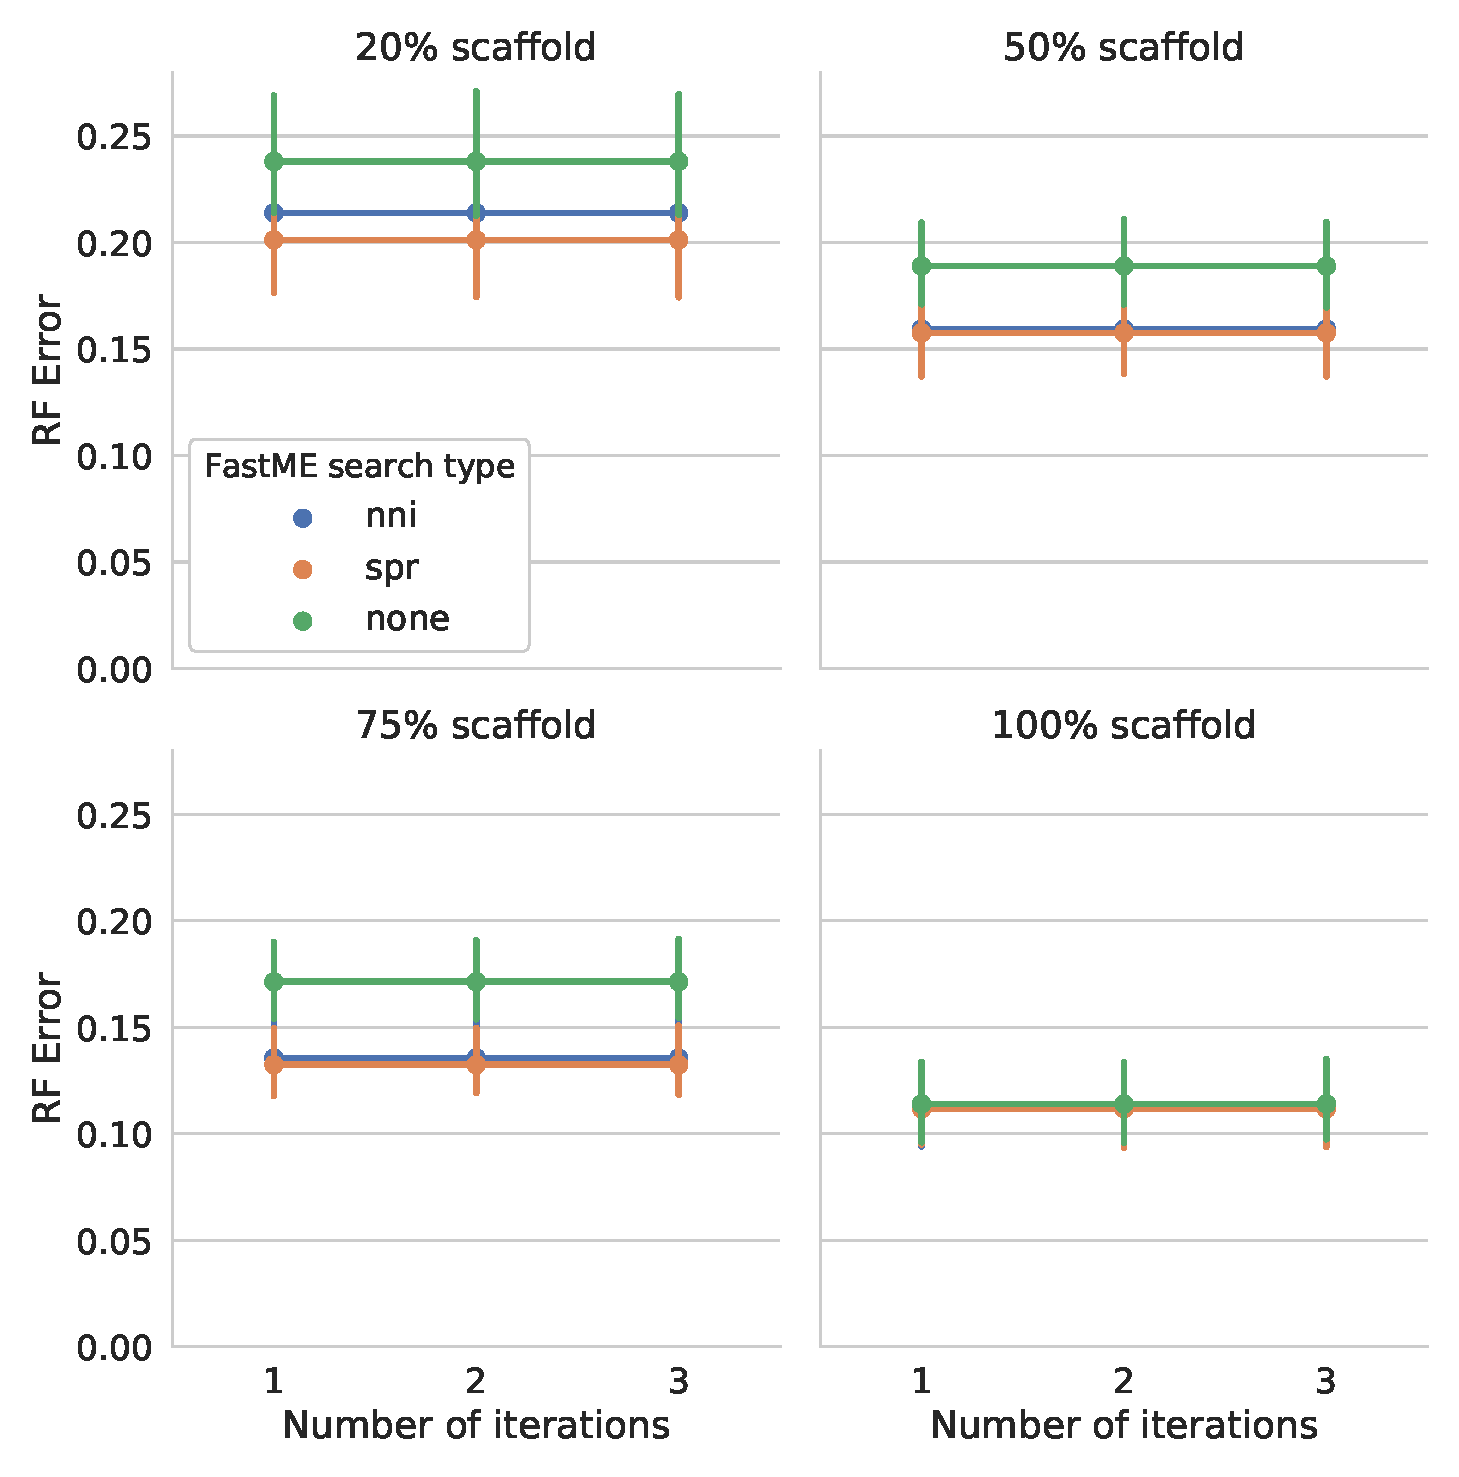
\includegraphics[height=3in]{astrid-missing-figs/iterations-err.eps}
    \caption{RF Error for 1000-taxon simulated datasets using up to 3 iterations of FastME with NNIs and FastME with SPRs. Each model condition has 10 replicates.}
    \label{astrid-missing::fig:iterations-err}
\end{figure}


\begin{figure}
    \centering
    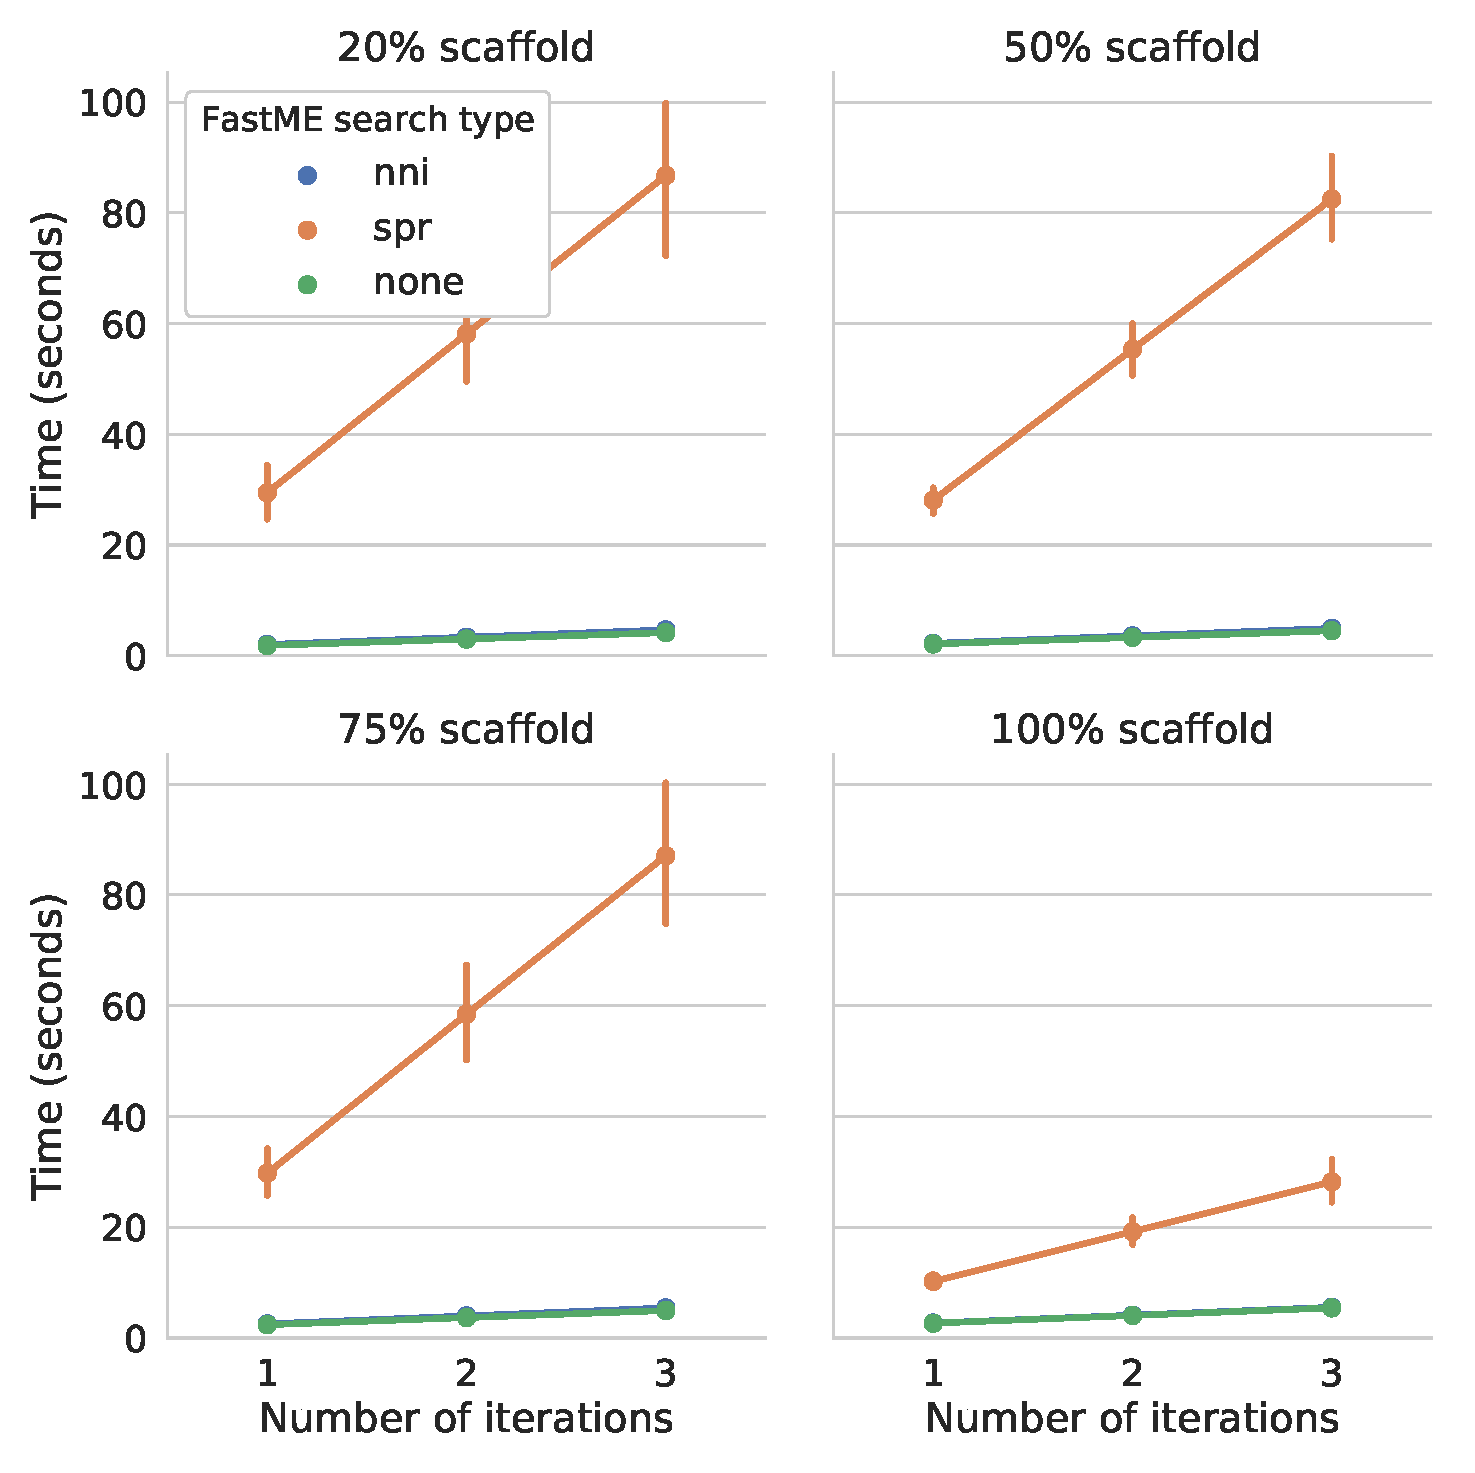
\includegraphics[width=\textwidth]{astrid-missing-figs/iterations-times.eps}
    \caption{Running times for 1000-taxon simulated datasets using up to 3 iterations of FastME with NNIs and FastME with SPRs. Each model condition has 10 replicates.}
    \label{astrid-missing::fig:iterations-times}
\end{figure}




%\part{Species Tree Estimation}
%\label{part:speciestree}

\chapter[Species Tree Estimation with ASTRID]{Species Tree Estimation with ASTRID\protect\footnotemark}\footnotetext{This chapter contains material previously published in \cite{vachaspati2015astrid}, which was a joint work with Tandy Warnow. It has been edited slightly for brevity. PV implemented ASTRID, performed experiments, wrote the first draft, and analyzed the data. TW designed the study, analyzed the data, and wrote the final draft.}
\label{chapter:astrid}



\section{Background}
% Species tree estimation in the presence of gene tree incongruence is a
% major challenge for many biological analyses. Gene tree incongruence
% can result from a variety of processes, notably incomplete lineage
% sorting (ILS) \cite{maddison1997gene}, which is modelled by the multispecies
% coalescent (MSC) \cite{Kingman1982}. 
% Concatenated
% maximum likelihood analyses is generally the most
% common method for species tree estimation
% from multiple loci, but can be statistically inconsistent,
% and even positively misleading, in
% some cases \cite{RochSteel-journal}, thus 
% converging to an incorrect tree 
% with increasing amounts of sequence data. 

% In recent years, a number of species
% tree estimation methods have been developed that are statistically
% consistent under the MSC, and so
% will converge in probability to the true species trees
% as the amount of data increases;
% see \cite{Degnan2009,liu2009coalescent,KnowlesKubatkoBook}.
% Methods that
% are statistically consistent under the MSC  include 
% ASTRAL \cite{ASTRAL}, ASTRAL-2
% \cite{ASTRALII},
% *BEAST \cite{StarBEAST},
% BEST \cite{BEST},  
% the population tree from BUCKy \cite{larget2010bucky},
% %Maximum Likelihood SuperTriplets \cite{MLST},
% METAL \cite{metal},
% MP-EST \cite{MPEST}, 
% NJst \cite{liu2011estimating},
% SNAPP \cite{bryant2012inferring}, 
% STEAC \cite{STEAC},
% %STAR \cite{STAR},
% STEM \cite{STEM}, and
% SVDquartets \cite{svdquartets}.
% While little is yet known about some of
% these methods (either because they have not yet
% been adequately studied or because
% they are not yet implemented), only a
% few of them (MP-EST, NJst, and ASTRAL-2)
% have been shown to be able to analyze very large datasets (especially
% those with large numbers of taxa) with high
% accuracy.
% MP-EST has been used more than either NJst or ASTRAL-2,
% but  NJst is more accurate than MP-EST, and ASTRAL-2 
% is more accurate than both  \cite{ASTRALII}.
% Furthermore, the currently available implementation of NJst is
% slower than ASTRAL-2, and cannot run on some datasets 
% \cite{ASTRALII,NJst}.

In this chapter, we present ASTRID, an ILS-aware distance-based
method for species tree estimation.  Our approach is based on NJst,
but is substantially faster, and, unlike NJst, functions even when
each gene tree contains only a small portion of the data.  The input
to NJst is a set of unrooted gene trees.
% each of which is required to
%have each of the $ n$ species.  
In the first step, an $n \times n$
matrix $D[x,y]$ is computed, where $D[x,y]$ is the average distance
(in terms of number of edges) between $x$ and $y$ among all the gene
trees.  In the second step, neighbor joining \cite{nj}, a very popular
distance-based method of phylogeny estimation, is used to produce the
species tree.  %As shown in \cite{NJst}, NJst is statistically
%consistent under the MSC model.


ASTRID improves on NJst  by
enabling other distance-based methods to be used in the second
step. In particular, although NJ cannot be run on datasets with missing
entries, other distance-based methods can, and ASTRID enables the use
of these other methods. We also explore the use of more accurate
distance-based methods. Thus, ASTRID is a very simple modification to NJst.
As we will show, ASTRID is much faster than NJst.

The comparison between ASTRID and ASTRAL-2 and MP-EST, two
established coalescent-based summary methods, is also interesting.
ASTRID
completed in minutes on some datasets where the other methods took hours, and
was fast enough to analyze datasets with 1000 species and 1000 genes on
a single processor within an hour (ASTRAL-2 and MP-EST take much more
time on datasets of this size).
Furthermore, 
ASTRID clearly dominates MP-EST in
terms of accuracy, and is competitive with ASTRAL-2 
(more accurate in some cases, and less accurate in others). 
Finally, ASTRID has desirable theoretical properties: 
it runs in polynomial time, and it remains 
statistically consistent under
the MSC model without assuming the molecular clock, nor requiring rooted gene
trees as input. 



\section{Methods}

\subsection{ASTRID}


The input to ASTRID is
a set of unrooted gene trees $T_1, \ldots, T_k$. We let 
$S_i=\mathcal{L}(T_i)$ denote the leafset of $T_i$, and
$S = \cup_i \mathcal{L}(T_i)$. Let $|S|=n$.

\begin{itemize}
\item[]{Step 1: Construct $n \times n$  matrix $\bar M$:}
\begin{enumerate}
\item For all $i=1,2,\ldots, k$, compute
$n \times n$ matrix $M_i$,
as follows. For pairs $p,q$  of species where both are
in  $S_i$, set $M_i(p,q)$ to be the
number of edges in
the path between $p$ and $q$ in $T_i$. 
For all other pairs $p,q$ (i.e., where
one or both are not in $S_i$), set $M_i(p,q) = 0$.
Thus, the only non-zero entries in $M_i$ are for pairs of
species in $T_i$.
\item For all $\{p,q\} \subset S$, let $n(p,q)$ be the
number of trees $T_i$ that contain both $p$ and $q$. 
\item Define $n \times n$ matrix  $\bar M$ by
setting $\bar M(p, q) =
\frac{\sum_i M_i(p,q)}{n(p,q)}$ if $n(p,q) >0$, and
  $\bar M[p,q] = -1$ (to denote a missing value) otherwise.
\end{enumerate}
\item[]{Step 2: Compute tree on $\bar M$ using a selected distance-based method}
\end{itemize}


\subsection{Datasets}
We tested species tree estimation methods on 
simulated datasets from previous publications, and also evaluated
ASTRID on the mammalian biological dataset of 37 species,
originally studied in \cite{statbinning}.
Here we briefly describe the simulation procedures used to
generate these datasets, and provide empirical
statistics for the datasets 
in Table \ref{astrid::table:datasets}.
See the original publications for details about the simulation protocols,
and our supplementary online materials at \url{https://pranj.al/ASTRID/} for links to the data.

All datasets
included both true and estimated gene trees, obtained by using maximum likelihood
methods on the true sequence alignments, as well as 
species trees estimated on these gene trees obtained in the
prior publications. 
Each gene tree had at most one copy of each species. 
We computed ASTRID 
species trees for these datasets, using various techniques for
Step 2 (how to compute the species tree given the distance matrix).

We estimated the amount of ILS in the data by quantifying the
average gene tree discord in the data, using the
average Robinson-Foulds (RF) \cite{RF} distance 
between true gene trees and the model species tree,
expressed as a percentage (written AD for ``average distance'').
We also explored some simulated datasets where the DNA sequence
evolution was under the strict molecular clock.
Model conditions with AD at most 25\% can be considered low ILS,
conditions with AD between 26\% and 39\% can be considered moderate ILS,
conditions with AD between 40\% and 59\% can be considered high ILS, and
conditions with AD of at least 60\% can be considered very high ILS. 
In Table \ref{astrid::table:datasets}, we indicate these  ILS levels for the different
model conditions we study both with the AD value, but also the general level (L for low,
M for moderate, H for high, and VH for very high).

\begin{table}
%\label{astrid::table:datasets}
  \begin{tabular}{| c | c | c | c | c | c|}
    \hline
    Dataset & \# genes & \# taxa & ILS level (AD\%) & \# sites & ref.\\       
    \hline
    \hline
    Avian very  high ILS (0.5X) & 1000 & 48 & 60 (VH) & 500 & \cite{statbinningdata}\\
    Avian high  ILS (1X) & 1000 & 48 & 47 (H) & 250-1500 & \cite{statbinningdata}\\
    Avian moderate (2X) & 1000 & 48 & 29 (M) & 500 & \cite{statbinningdata}\\
    \hline
    Mammalian  high ILS (0.5X) & 200 & 37 & 50 (H) & 250-1000 & \cite{statbinningdata}\\
    Mammalian moderate ILS (1X) & 200 & 37 & 29 (M) & 250-1000 & \cite{statbinningdata}\\
    Mammalian low ILS (2X) & 200 & 37 & 21 (L) & 250-1000 & \cite{statbinningdata}\\
    \hline
    10-taxon very high ILS & 200 & 10 & 89(VH)  &  100 & \cite{bayzid2014weighted}\\
    10-taxon high ILS  & 200 & 10 & 48 (H) &  100 &\cite{bayzid2014weighted}\\
    \hline
    15-taxon clocklike  & 1000 & 15 & 82 (VH) & 100-1000 & \cite{bayzid2014weighted}\\
    \hline
    ASTRAL-2 500K-1e6 (MC1) & 1000 & 200 & 69 (VH) & 300-1500& \cite{ASTRALII}\\   
    ASTRAL-2 2M-1e6 (MC2) & 1000 & 200 & 33 (M) & 300-1500& \cite{ASTRALII}\\   
    ASTRAL-2 10M-1e6 (MC3) & 1000 & 200 & 21 (L)  & 300-1500& \cite{ASTRALII}\\
    ASTRAL-2 500K-1e7 (MC4) & 1000 & 200 & 68 (VH) & 300-1500& \cite{ASTRALII}\\
 ASTRAL-2 2M-1e7 (MC5) & 1000 & 200 & 34 (M) & 300-1500& \cite{ASTRALII}\\
ASTRAL-2 10M-1e7 (MC6) & 1000 & 200 & 9  (L) & 300-1500& \cite{ASTRALII}\\
    ASTRAL-2 2M-1e6 (MC7) & 1000 & 10 & 17 (L) & 300-1500& \cite{ASTRALII}\\
    ASTRAL-2 2M-1e6 (MC8) & 1000 & 50 & 30 (M) & 300-1500& \cite{ASTRALII}\\
    ASTRAL-2 2M-1e6 (MC9) & 1000 & 100 & 34 (M) & 300-1500& \cite{ASTRALII}\\
    ASTRAL-2 2M-1e6 (MC10)& 1000 & 500 & 34 (M) & 300-1500& \cite{ASTRALII}\\ 
    ASTRAL-2 2M-1e6 (MC11) & 1000 & 1000 & 35 (M) & 300-1500& \cite{ASTRALII}\\ 
    \hline
  \end{tabular}
\caption[Empirical statistics of simulated datasets used in ASTRID
    study.]{Empirical statistics of simulated datasets used in this
    study. {\rm The ILS level 
is measured by the average Robinson-Foulds distance (AD) between the true
  gene trees and the species tree, expressed as a percentage; ILS levels
are then classified as low (L), moderate (M), high (H), or very high (VH).
% ASTRAL-2 datasets
%labelled MC1-MC6 correspond to datasets with 200 taxa.
}
} 
\label{astrid::table:datasets}
\end{table}

\subsubsection{Mammalian and avian simulated datasets}

These datasets were created  in \cite{statbinningdata}
to evaluate method performance under model conditions similar to real
data. 
Species trees were generated with MP-EST for the
avian phylogenomics dataset with 48 species and 14,446 loci
\cite{jarvis2014whole}, and for a mammalian dataset with 37 species
and 447 loci \cite{song2012resolving}. 
These species trees were used as basic model trees, with
branch lengths in coalescent units.
  In addition, two other
model species trees were created for each dataset by
scaling the species tree branch lengths up (to reduce ILS) or down
(to increase ILS).  The ILS levels of the resultant model species trees were very
heterogeneous, ranging from AD = 21\% (low) to 50\% (high) for
the mammalian simulation, and from AD = 29\% (moderate) to 60\% (very high) for
the avian simulation.

Both datasets had sequences of length 500 for all three model
conditions. For the default (``1X'') branch length condition, the
avian dataset also had sequences of length 250, 500, 100, and 1500,
and the mammalian dataset had sequences of length 250, 500 and 1000.
Sequence evolution on these datasets deviated from the strict
molecular clock.

\subsubsection{10-taxon simulated datasets}
These data were presented in 
\cite{bayzid2014weighted}, and explored two ILS 
levels (AD=48\% (high) and AD=89\% (very high)). Sequence evolution deviated
from the strict molecular clock. 

\subsubsection{15-taxon clocklike simulated datasets}
These datasets evolved under a strict molecular clock, and
were presented in
\cite{bayzid2014weighted}.  The species tree was a
caterpillar model tree (i.e., a path with leaves hanging off the
path) with very short internal branches,
and a long branch to the outgroup species. 
The ILS level in these data was very high (AD=82\%).






\subsubsection{ASTRAL-2 simulated datasets}
These data were presented in \cite{ASTRALII}, and provided a
variety of model conditions with varying ILS levels, tree shapes,
numbers of taxa, and sequence lengths per locus.  
SimPhy \cite{SimPhy} was used to generate the species
and gene trees, based on
two parameters: the number of generations (given as the
first number in the model)
and the speciation rate (given as the second
number).   %for the 200-taxon data. 
The number of generations simulated ranged between
  500K, 2M, and 10M, and
  the speciation rate varied between  1e6 and 1e7.
  Model conditions with fewer generations had more ILS.
  Model conditions with the 1e6 speciation rate had speciation events
  nearer the tips (leaves) of the trees, while model conditions with the 1e7
  speciation rate had speciation events nearer the root.
The ILS levels varied from very low (AD = 9\%) to 
very high (AD = 69\%).
Sequences evolved down the gene trees under 
multiple  GTRGAMMA models that deviated from the strict
molecular clock. 
Maximum likelihood gene trees were computed using FastTree-2.
\subsubsection{Incomplete gene tree datasets}
To explore performance on incomplete gene trees, 
we modified the ASTRAL-2 dataset by randomly removing taxa from trees
in the  50-taxon datasets. Up to 40 taxa were removed from the
50-taxon dataset, and up to 5 taxa were removed from the 10-taxon
dataset. In each of these cases, 
maximum likelihood gene trees were estimated using
FastTree-2 version 2.1.7 SSE3 \cite{Price2010}, using the following
command:
\begin{verbatim}
fasttree -nt -gtr -quiet -nopr -gamma -n 1000  <fastafile> > <genetreefile>
\end{verbatim}
\noindent
where {\tt <fastafile>} was the input file of aligned sequences and {\tt <genetreefile>} was the output file.

\subsection{Distance-based tree estimation methods}
In order to explore the design space for ASTRID, we 
ran various distance-based methods for Step 2 (computing the
tree from the distance matrix).
For incomplete distance matrices (where some entries
are $-1$, indicating that the pair of taxa do not
appear together in any gene tree), we explored the
methods  in PhyD* \cite{phydstar}: $NJ*$, $BIONJ*$, $MVR*$,
$UNJ*$. These
algorithms are all variants on neighbor joining that work on incomplete distance matrices.
We also explored
$FASTME$ \cite{Desper2002}, which is a heuristic for the
minimum 
evolution problem.

\subsection{ASTRAL-2}
To compute ASTRAL-2 species trees on the incomplete gene trees
generated for the ASTRAL-2 datasets, 
we ran ASTRAL-2 version 4.7.8, using command line arguments 
\begin{verbatim}
java -Xmx4000M -jar astral.4.7.8.jar -i <genetrees> -o <outputtree>
\end{verbatim}

\subsection{Computing tree error}
All trees computed in this study were fully resolved. 
We report the RF tree error (the proportion of the
branches in the model tree missing from the estimated tree),
using scripts that 
are available in the supplementary online
materials at \url{https://pranj.al/ASTRID/}. 

\section{Results}


\subsection{Selection of distance-based tree estimation method for Step 2}

First, we evaluated various distance-based tree estimation methods to
determine which one would be most accurate for the tree computation
phase of ASTRID.  
Results on datasets with all complete gene trees (no missing species
in any gene) are shown in 
Figure \ref{astrid::fig:avian-njcomparison}
and results on datasets with incomplete gene trees
are shown in Figure \ref{astrid::fig:astral2-missing-njcomparison-main-l300}.
Note that
for datasets with entirely complete gene trees, 
FastME performed as well as or better than the other
distance-based methods, but
there were datasets with incomplete distance matrices
in which FastME had very poor accuracy. 
Therefore, 
we selected FastME to analyze datasets where the
distance matrix has no missing entries, since it had the
best accuracy. For the datasets with incomplete distance matrices
$\bar M$ (indicated by $\bar M[p,q]=-1$ for some p,q), we
selected
BioNJ*, since it generally had among the most
accurate results of these PhyD* methods.
\begin{figure}
  \centering
  \includegraphics[width=12cm]{astrid-figs/avian-njcomparison.eps}
  \caption[Comparison of  ASTRID variants on
moderate ILS avian simulated datasets]{\textbf{A comparison of ASTRID variants on the
moderate ILS avian simulated datasets with 500bp, using 
different distance-based methods for the
      tree estimation phase.}
    We report RF topological error rates over 20 replicates. Red dots
    represent means, while lines represent medians and boxes represent
    quartiles. 
}
  \label{astrid::fig:avian-njcomparison}
\end{figure}


\begin{figure}
  \centering
  \includegraphics[width=12cm]{astrid-figs/astral2-missing-l300-njcomparison-main.eps}
  \caption[Comparison of ASTRID variants
on 50-taxon datasets with missing taxa.]{\textbf{Comparison of ASTRID variants
on 50-taxon ASTRAL-2 MC8 datasets with missing taxa.}
 We show
average RF error rates over 50 replicates for
ASTRID variants, that differ in terms of the method used
to compute the tree from the distance matrix. 
The datasets have  taxa randomly removed
    from each gene and the sequence lengths truncated to 300bp. 
    Red dots
    represent means, while lines represent medians and boxes represent
    quartiles.}
  \label{astrid::fig:astral2-missing-njcomparison-main-l300}
\end{figure}


\subsection{Comparison of ASTRID, ASTRAL, and MP-EST}


We begin with a comparison between ASTRID, ASTRAL-2, and MP-EST 
on the avian simulated datasets with high (1X) ILS, varying number
of genes  and sequence alignment lengths, but where
all genes are complete; see Figure \ref{astrid::fig:avian-mpest}.

\begin{figure}
  \centering
  \includegraphics[width=12cm]{astrid-figs/avian-mpest.eps}
  \caption[Comparison of ASTRID, ASTRAL-2, and MP-EST 
      on avian simulated data]{\textbf{Comparison of ASTRID, ASTRAL-2, and MP-EST 
      on the avian simulated data.} The
simulated data evolve under 1X (high ILS) species tree branch lengths,
and with
      varying gene sequence lengths.
      We report mean RF rates with standard error bars over 20
    replicates. 
}
  \label{astrid::fig:avian-mpest}
\end{figure}
All methods improved with increasing numbers of genes
or increasing sequence length; however, the methods
differed substantially in terms of their accuracy.
Across all conditions we explored,
MP-EST had the highest error 
and ASTRID had the lowest  error. 
ASTRAL-2 was in between, but was closer to ASTRID than to 
MP-EST. 
The gap between MP-EST and ASTRID was very large,
and increased with the number of genes. For example,
at 1000 genes and gene sequence alignments of length 500,
MP-EST had 19\% RF error while
ASTRID had about 7\% RF error.
The gap between ASTRID and ASTRAL-2 was substantial 
on the 200- and 500-gene cases, but very small
on the 1000-gene case. 

Thus, although MP-EST is statistically consistent
under the MSC model
and hence theoretically robust to ILS, it 
did not have particularly good accuracy on
these data. 
Among all coalescent-based methods, 
MP-EST is probably the one that has been used the
most in biological data analyses, but
its performance here and
in \cite{ASTRALII,BayzidRECOMBCG2014} demonstrates that it is not
competitive with the best methods on  datasets
with even moderate numbers
of species. 
Therefore, we omit MP-EST from the rest of
this study.




\subsection{Comparison of ASTRID and ASTRAL-2 
on complete gene trees}

\paragraph{Comparison on avian datasets. }
Figure \ref{astrid::fig:avian-ils} shows the performance of
ASTRAL-2 
 and ASTRID on avian simulated datasets
under three ILS conditions (moderate, high, and very high).
Both methods performed better when provided with more genes, and both
performed worse on higher levels of ILS.
Overall, ASTRID tended to outperform ASTRAL-2, with the
largest effect seen when many genes were available. With 800 genes
available, the ASTRID species tree had a RF error
rate that was 2.4 percentage points better than ASTRAL-2’s under the
very high and high ILS model conditions, and 1.2 percentage points better for
the moderate ILS model condition.
On the moderate ILS model condition, ASTRID had the greatest advantage
over ASTRAL-2 
 for moderate numbers of genes. Above 200 genes, the error
rate dropped below ten percent for both ASTRAL-2 
 and ASTRID, and ASTRID
had an average advantage of only about one percentage point.


\begin{figure}
  \centering
  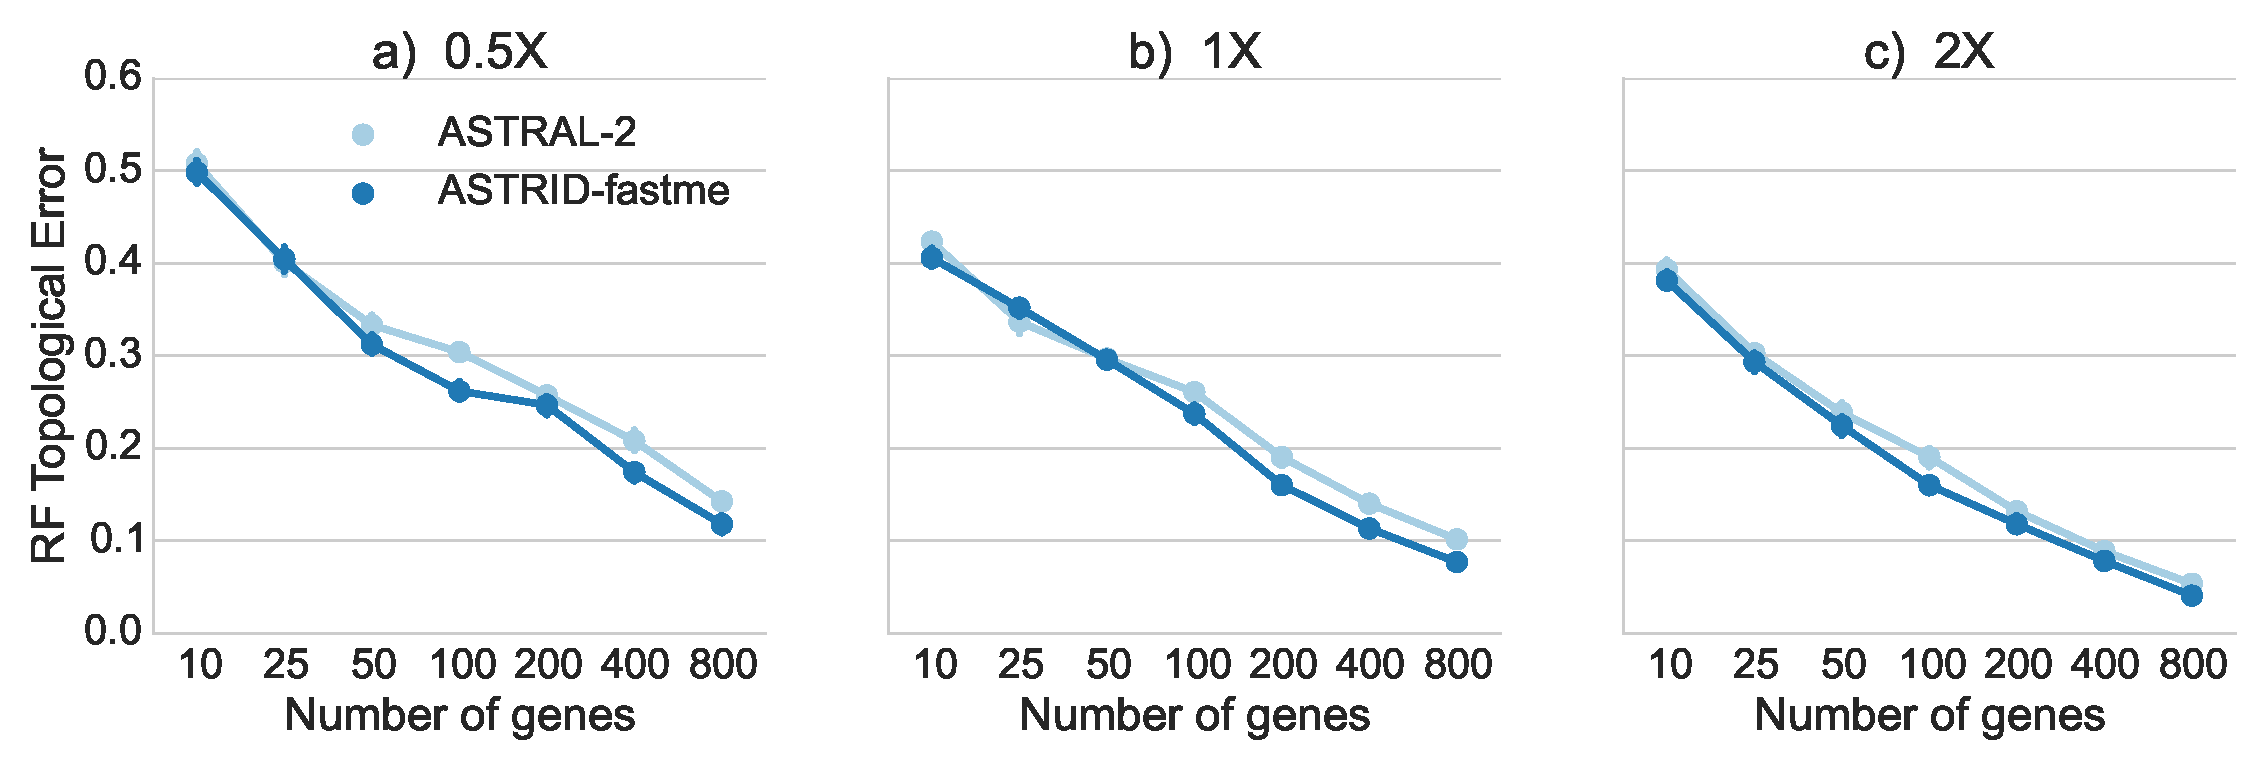
\includegraphics[width=12cm]{astrid-figs/avian-ils.eps}
  \caption[Comparison of ASTRID and ASTRAL-2 on avian simulated datasets]{\textbf{Comparison of ASTRID and ASTRAL-2 on avian simulated datasets. }
We show average RF error rates and standard error
bars for 20 replicates. Gene sequence alignments  have 500 sites
and
    varying amount of ILS. 
Species tree branch lengths of 0.5x 
    have very high ILS, 1X has high ILS, and 2x have moderate ILS. 
}
  \label{astrid::fig:avian-ils}
\end{figure}


It is well known that summary methods improve in accuracy as the
number of sites per gene or the number of genes increase
\cite{mirarab2014evaluating,GatesyMPE2014,bayzid2013naive,roch2015robustness}.  We
explored the impact of varying the sequence length and number of genes
on the avian datasets with high (1X) ILS, as well as on true gene
trees.  Figure \ref{astrid::fig:avian-seqlength} shows results on 10, 100, and
1000 genes; results on other numbers of genes have the same trends
(data provided in supplementary materials at \url{https://pranj.al/ASTRID/}).
As expected, both methods improved
with increased sequence length, and had their best accuracy on
true gene trees.
Both methods also improved as the number of genes increased. 
ASTRID
was always at least as accurate as ASTRAL-2,
with the biggest improvement for shortest
sequences (with 250bp). 
 

\begin{figure}
  \centering
  \includegraphics[width=12cm]{astrid-figs/avian-seqlength-main.eps}
  \caption[Performance on the avian simulated data with 1X
      species tree branch lengths]{\textbf{Performance on the avian simulated data with 1X
      species tree branch lengths, varying gene sequence length and
      number of genes.} We report RF  rates over 20
    replicates.}
  \label{astrid::fig:avian-seqlength}
\end{figure}

\paragraph{Comparison on mammalian datasets. }
A comparison of ASTRAL-2 
 and ASTRID on the mammalian datasets
with different levels of ILS (high, moderate, and low)
is given in 
Figure \ref{astrid::fig:mammalian-ils}.
ASTRAL-2 
 and ASTRID performed
fairly similarly on the low (2X branch lengths) and moderate (1X branch
lengths) ILS conditions. Under the high ILS level (0.5X branch lengths), ASTRAL-2 
 was fairly consistently more accurate than ASTRID, with the largest
improvement on the 10-gene case.

\begin{figure}
  \centering
  \includegraphics[width=12cm]{astrid-figs/mammalian-ils.eps}
  \caption[Comparison of methods on mammalian simulated datasets, varying ILS level and number of genes]{\textbf{Comparison of methods on mammalian simulated datasets, varying ILS level and number of genes.}  We
show average RF error rates and standard error bars for 20 replicates. 
Gene sequence alignments had
    500 sites. Model conditions varied in ILS level
from high (0.5x branch lengths) to low (2X branch lengths).
}
  \label{astrid::fig:mammalian-ils}
\end{figure}

\paragraph{Comparison on the ASTRAL-2 datasets. }
We explored performance on the ASTRAL-2 datasets
with 200 taxa (model conditions MC1 to MC6, see
Fig.~\ref{astrid::fig:astral2-ils}). % (i.e., MC1-MC6).
These model trees varied in ILS level, with MC1 and MC4 having 
very high ILS, MC2 and MC5 having moderate ILS, and
MC3 and MC6 having low ILS. 
Under MC2, MC3, and MC5, the two methods had 
essentially identical accuracy. However, under MC1, MC4, and MC6, 
ASTRAL-2 had an advantage over ASTRID.
In MC1 and MC4, the improvement disappeared at 100 genes,
but in MC6 ASTRAL-2 was still more accurate than ASTRID on 100 genes.


\begin{figure}
  \centering
  \includegraphics[width=12cm]{astrid-figs/astral2-ils.eps}
  \caption[Comparison of ASTRID and ASTRAL-2
 on the simulated ASTRAL-2 datasets]{\textbf{Comparison of ASTRID and ASTRAL-2
 on the simulated ASTRAL-2 datasets
      with 200 taxa, varying levels of ILS, tree shape, and number of genes.}
    %Speciation events in the $1e-6$ model condition tended to occur
    %near the tips of the tree, and speciation events in the $1e-7$
    %model condition tended to occur near the root. Fewer generations
    %correspond to higher levels of ILS. 
     We report RF error
    rates and standard error 
bars over 10 replicates. See Table \ref{astrid::table:datasets} for
information on the model conditions listed. }
  \label{astrid::fig:astral2-ils}
\end{figure}

\paragraph{Comparison  on the 15-taxon datasets. }
%Tandy - check multiple-labels
The 15-taxon datasets evolved on a caterpillar
species tree under very high ILS (AD=82\%), the highest
ILS considered in this study.
We explored performance under two sequence lengths (100bp and 1000bp)
and varied the number of genes from 10 to 1000. 
Results on the 15-taxon datasets (Fig.~\ref{astrid::fig:15taxon})
showed very close performance between ASTRID and ASTRAL-2.
On the 100bp alignments and on 1000bp alignments with
at least 100 genes, the  two methods could not be distinguished.
However, on 1000bp alignments with at most 50 genes, ASTRAL-2
had an advantage over ASTRID.
\begin{figure}
  \centering
  \includegraphics[width=12cm]{astrid-figs/15-taxon.eps}
  \caption[Comparison of ASTRID and ASTRAL-2  on the 15-taxon simulated
      datasets for two different sequence lengths]{\textbf{A comparison of ASTRID and ASTRAL-2  on the 15-taxon simulated
      datasets for two different sequence lengths.} The 15-taxon datasets
evolve down gene trees generated by a caterpillar
tree with very high ILS (AD=82\%), the highest ILS condition
explored in this study. We report mean RF 
      rates and standard error over 10 replicates. 
}  
  \label{astrid::fig:15taxon}
\end{figure}

\paragraph{Comparison on the 10-taxon datasets. }
The 10-taxon datasets evolved under two different ILS levels - high
and very high, and we explored performance  on both true and
estimated
gene trees; see Figure \ref{astrid::fig:10-taxon}.
In general, ASTRID and ASTRAL-2 had very close accuracy
on these data, but
there were some cases where they had different accuracy levels.
For example, on the high ILS condition with estimated
gene trees, ASTRAL-2 
 was more accurate 
than ASTRID for 200 genes, and ASTRID was
more accurate than ASTRAL-2 
 on 25 genes.





\begin{figure}
  \centering
  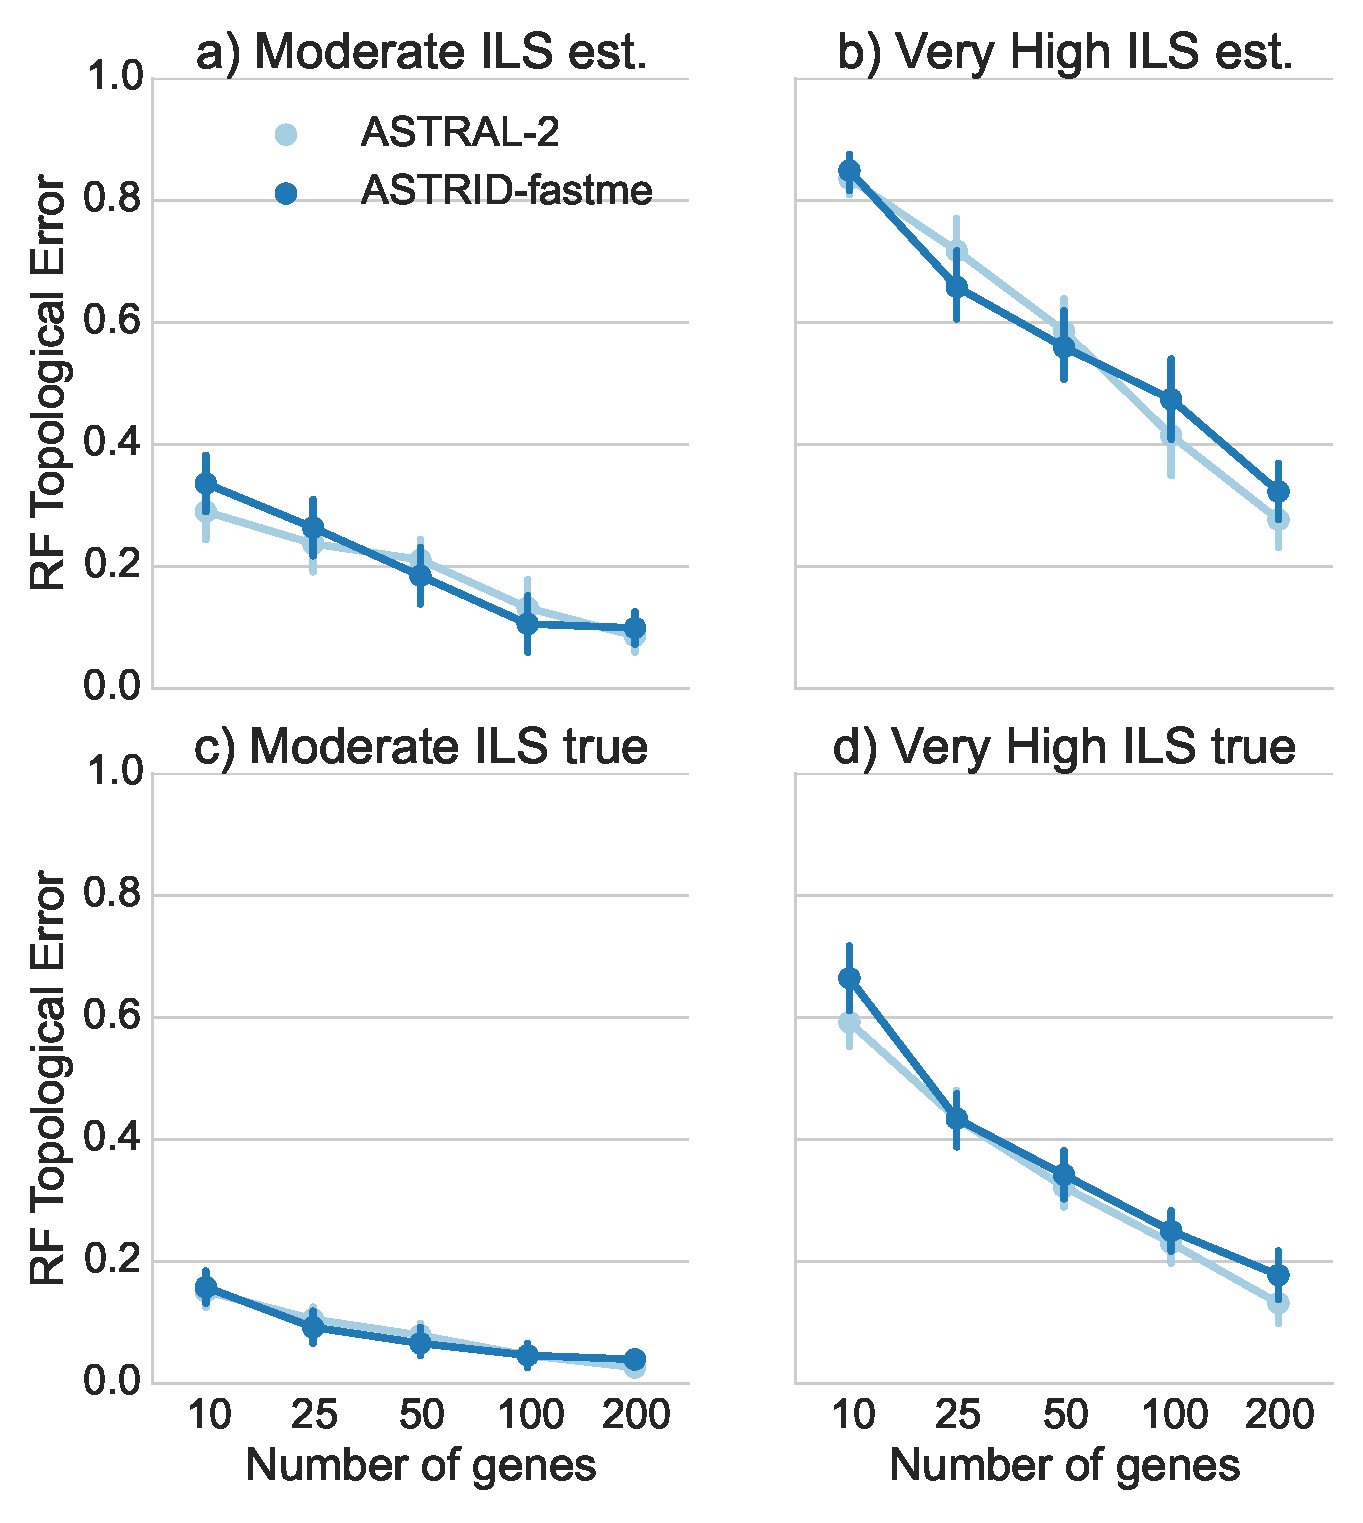
\includegraphics[width=12cm]{astrid-figs/10-taxon.eps}
  \caption[Results on true and estimated gene trees on 10-taxon datasets
with two ILS levels]{\textbf{Results on true and estimated gene trees on 10-taxon datasets
with two ILS levels (high and very high).}
      All gene sequence alignments have 100bp. We report RF rates and standard error bars over 20
    replicates. 
}
  \label{astrid::fig:10-taxon}
\end{figure}


\subsection{Performance on incomplete gene trees}
We explored the impact of missing data on
ASTRAL-2 and ASTRID by deleting taxa from gene trees
in the 
50-taxon datasets (MC8) from the ASTRAL-2 collection, 
using
150bp per gene, and varying the
number of genes and the amount of missing taxa; see Figure
\ref{astrid::fig:astral2-missing}. 
ASTRAL-2 
 and ASTRID had 
very similar 
topological accuracy throughout
these experiments. With low amounts of
missing data (20\% to 40\% missing taxa from each
gene tree), both methods had very good
accuracy (below 5\% tree error) by 500
genes. With 60\%  of the taxa missing from each gene tree,
the error rates increased for low
numbers of genes (above 20\% RF error for
up to 100 genes), but then declined to about 10\% by
1000 genes. 
With 80\% of the taxa missing from
each gene (so that all gene trees have only 10 taxa out of 50),
error rates were very high with 
25 genes (at least 85\% RF), but decreased quickly with increases
in the number of genes, so that
at 500 genes the error rate was 24\%, and
then at most 18\% at 1000 genes.
The trends suggest that
the error rates had not plateaued, and that adding additional
incomplete gene trees should result in continued improvement.

\begin{figure}
  \centering
  \includegraphics[width=12cm]{astrid-figs/astral2-missing.eps}
  \caption[Results on 50-taxon ASTRAL-2 dataset with
missing  taxa ]{\textbf{Results on 50-taxon ASTRAL-2 dataset (MC8) with
missing  taxa 
    and sequence lengths of 150bp.} We
    report RF rates and standard error over 50 replicates. 
}
  \label{astrid::fig:astral2-missing}
\end{figure}



\subsection{Analysis of the mammalian biological dataset}
We analyzed the mammalian biological dataset originally
studied in \cite{song2012resolving}.  
The original
dataset had 37 species and 447 genes, but
there were 23
erroneous genes (as noted by \cite{statbinning}) which
we removed before doing the analysis. 

We obtained maximum likelihood gene trees and bootstrap
replicates of these gene trees from \cite{mirarab2014statistical}.
We then analyzed these
data using ASTRAL-2 and ASTRID+FastME
and compared these analyses to 
previously published trees obtained using ASTRAL
and MP-EST \cite{ASTRAL}. 
We then annotated the branches of the ASTRID+FastME and ASTRAL-2 trees with
bootstrap support from 100 multi-locus bootstrapping (MLBS).
The ASTRID+FastME and ASTRAL-2 trees
were topologically identical to the ASTRAL tree and differed
only in the bootstrap support;  
see Figure \ref{astrid::fig:astrid-biological} for the ASTRID+FastME tree.
On the other hand, the support for
the placement of Scandentia - one of the major
open questions about mammalian evolution - was very low,
only 47\% (ASTRAL-2 gave it 82\%). 
Hence, neither the ASTRID tree nor the ASTRAL-2 tree
resolved the placement of Scandentia
with high support.


\begin{figure}
\centering
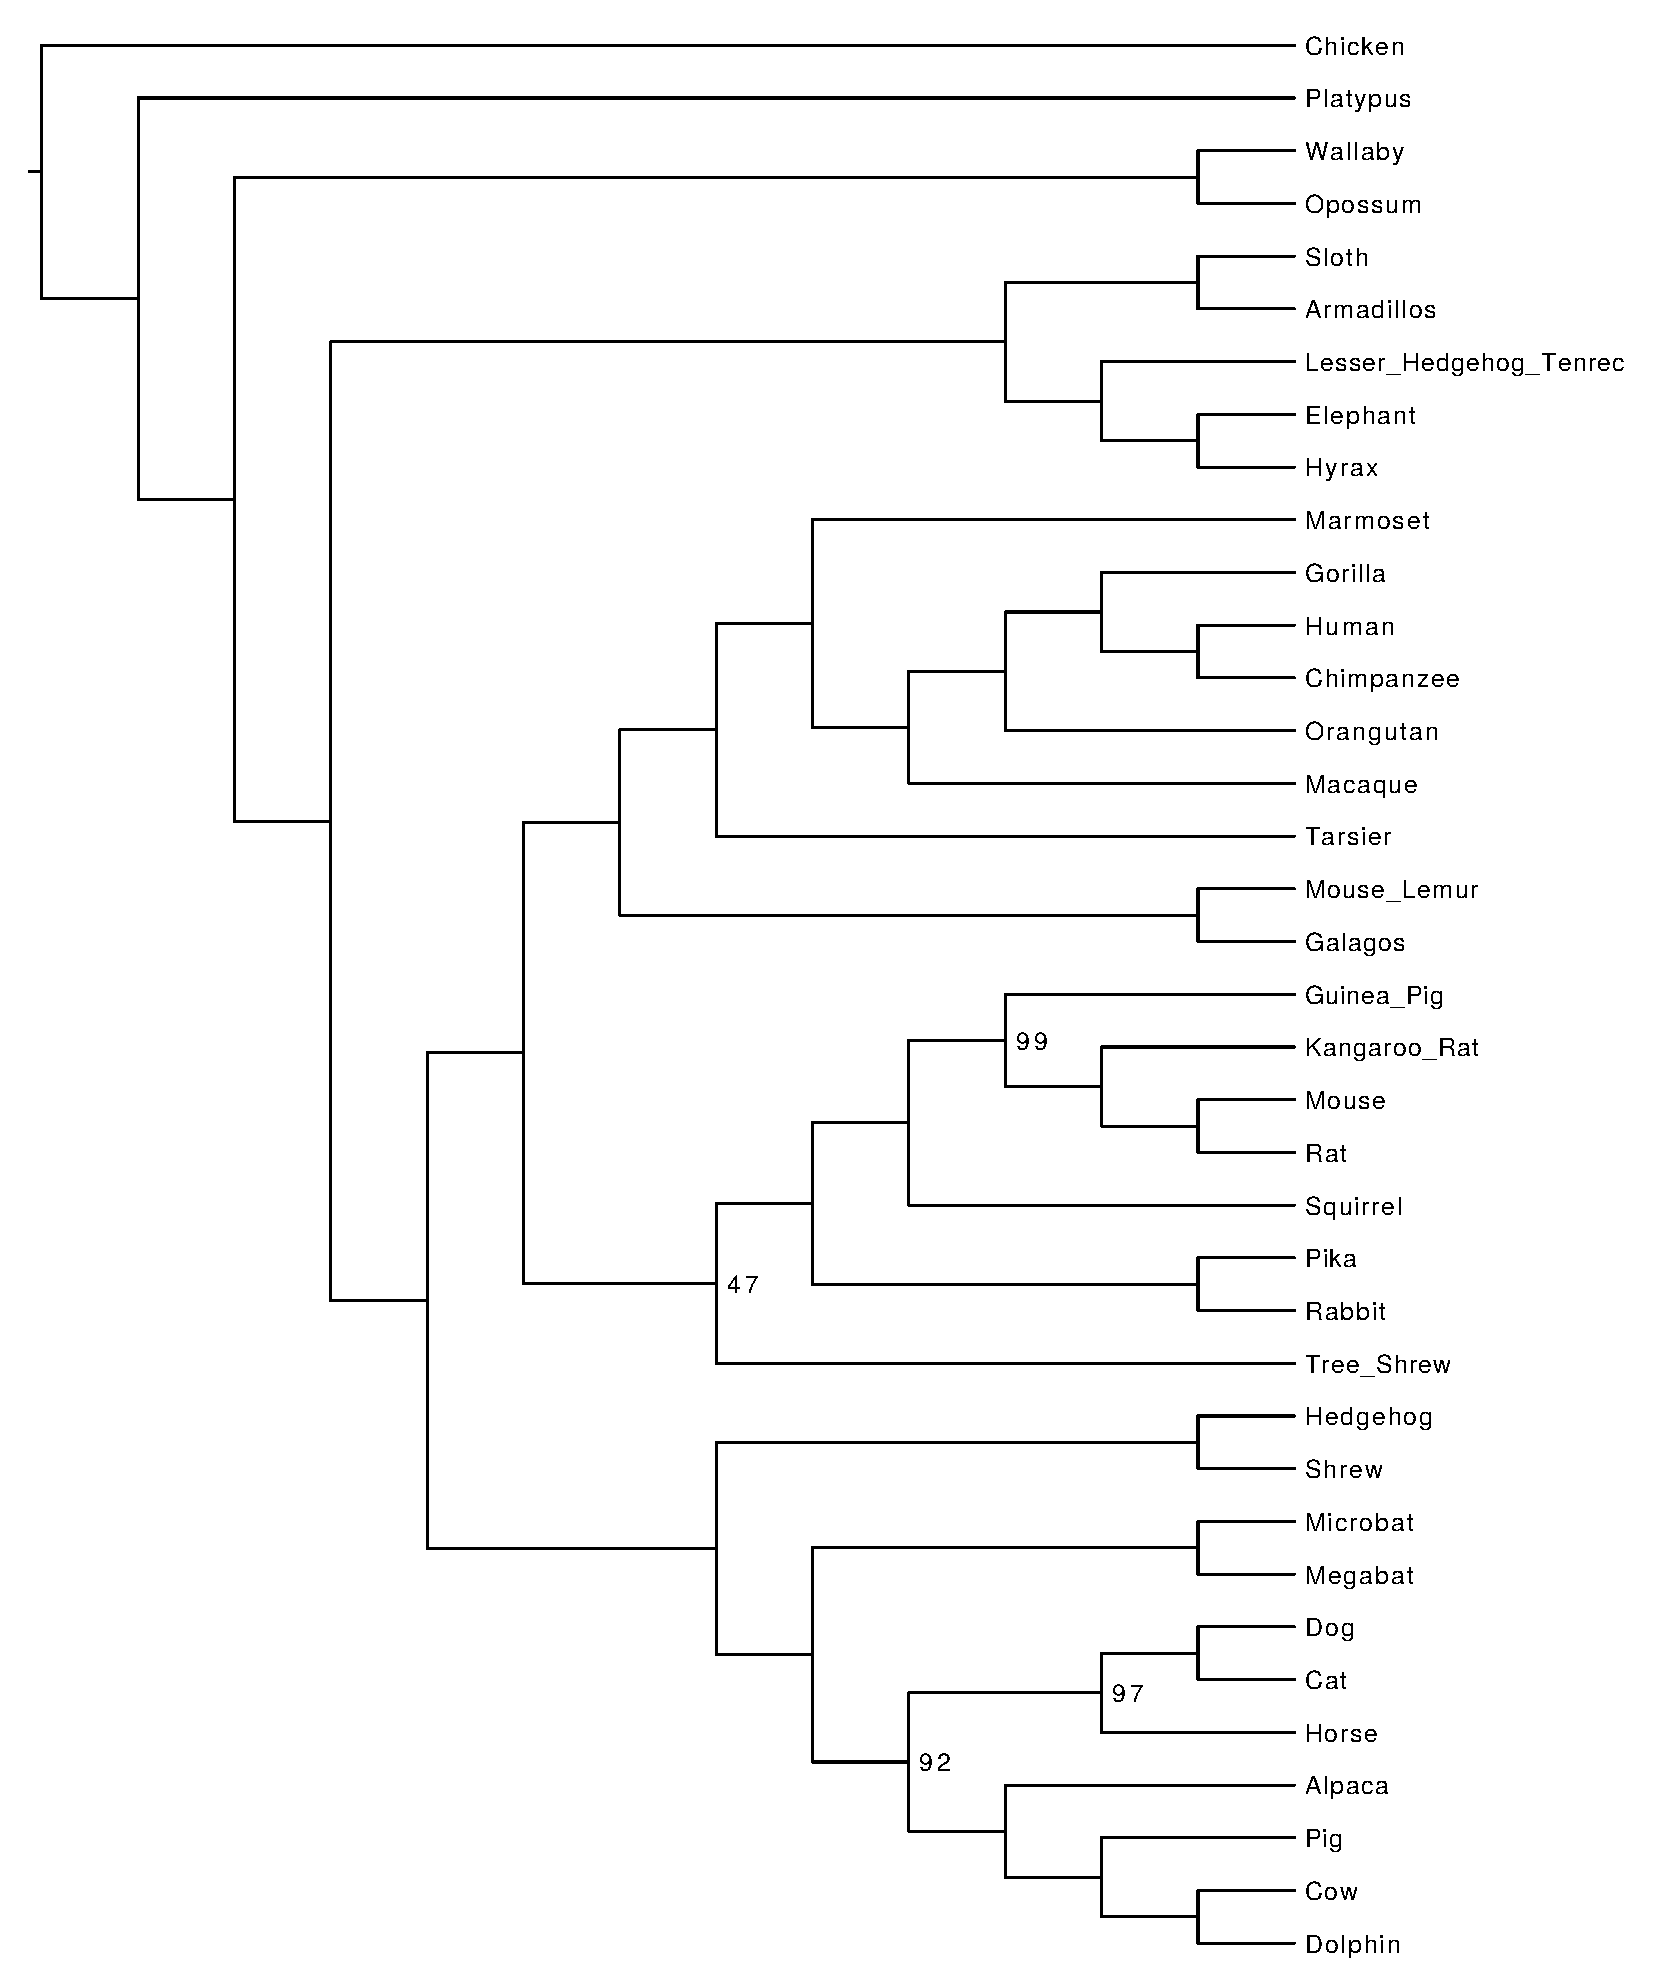
\includegraphics[width=12cm]{astrid-figs/astrid-biological.eps}
%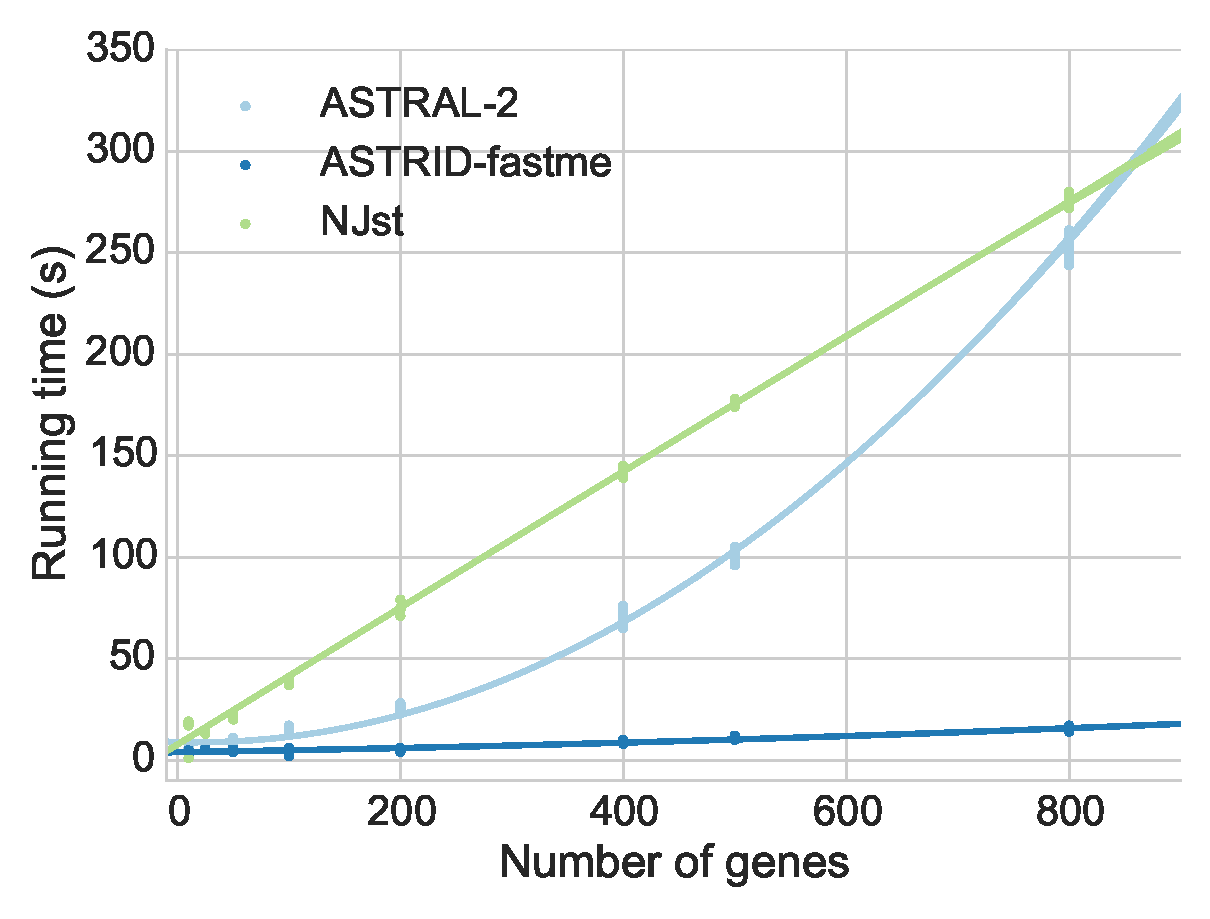
\includegraphics[width=12cm]{astrid-figs/avian-timing.eps}
  \caption[ASTRID analysis of a mammalian
biological dataset]{\textbf{ASTRID analysis of a mammalian
biological dataset.} 
We used ASTRID+FastME to 
analyze the mammalian biological dataset 
studied in \cite{statbinning,ASTRAL}, with 37 taxa and
424 genes. 
The branches are
annotated with 
bootstrap support values from 100 MLBS bootstrap samples;
values not shown indicate 100\% support.
The ASTRID tree is identical to the ASTRAL and ASTRAL-2 trees on the same data,
but differs from the MP-EST analysis in the placement of Scandentia.}
  \label{astrid::fig:astrid-biological}
\end{figure}




\subsection{Running time results}

\subsection{Asymptotic running time}

ASTRID has two steps: the first step computes the distance matrix, and
the second step uses a selected distance-based method to construct a
tree from the distance matrix.  When the input has $n$ species and $k$
genes, then calculating the distance matrix can be performed in
$O(kn^2)$ time.  Distance-based tree estimation methods typically run
in $O(n^2)$  to $O(n^3)$ time, but this step no longer depends on $k$.
Hence, the overall running time depends on the selected distance-based
method, but is generally dominated by the first phase, especially for
typical inputs, for which $k >> n$. Thus, under the assumption that
$k > n$ and that ASTRID uses a distance-based
method that runs in $O(n^3)$ time, ASTRID’s running time is $O(kn^2)$.

ASTRAL-2's scaling is more complicated to discuss.
Asymptotically, ASTRAL-2 runs in $O(n k |X|^2)$ time, where
$n$ is the number of species, $k$ is the number of genes, and $X$ is
a set of bipartitions it computes to constrain
the search space. The size of $X$ is not bounded by a polynomial
in the input size, and the technique that ASTRAL-2 uses
means that $X$ can be large under conditions with
high ILS. 
Thus the asymptotic running times of ASTRAL-2 and ASTRID (used with
various distance methods) are quite 
different. 

\subsection{Running times on simulated data}
In practice, creating the distance matrix took the majority of the
running time. On 1000 taxa, creating the distance matrix took several
minutes to several hours, depending on the number of genes, but
running $FASTME$ took less than one second regardless of the number of
genes. However,  PhyD* methods were much
slower than $FASTME$; on 1000 taxa, running any of the PhyD* methods
took approximately 40 minutes (data not shown).




We recorded running
times for ASTRAL-2, 
ASTRID-FastME, and NJst, 
on avian 
simulated datasets with high ILS (1X),
as
we varied the number of genes (see Fig.~\ref{astrid::fig:avian-timing}).
Note that ASTRID-FastME was by far the fastest of the three
methods, and NJst was the slowest. However, the trends suggest
that NJst will be faster than ASTRAL-2 for larger numbers of genes.
Note also that ASTRID-FastME and NJst both scaled linearly with the
number of genes, but that ASTRAL-2’s running time scaled super-linearly.

We recorded running times for two variants of ASTRID
(one using FastME and the other using BioNJ*), and compared them
to ASTRAL-2 on ASTRAL-2 simulated datasets  with
1000 taxa (MC11) as we varied the number of genes
(Fig.~\ref{astrid::fig:1000-timing}) and for 500-gene datasets
in which we varied the number of taxa (MC 2 and 7-10, see Fig.~\ref{astrid::fig:astral-timing}).
The relative running times show that all methods were
very fast for smaller datasets, but were clearly distinguished
on the larger datasets, where 
ASTRID-FastME was much faster than ASTRID-BioNJ* and 
both variants of 
ASTRID were much faster than ASTRAL-2.  
For example, on the dataset with 1000
genes and 1000 taxa, ASTRID-FastME
finished in 33 minutes, ASTRID-BioNJ finished in 1 hour and 10
minutes, and ASTRAL-2 finished in 12 hours and 30 minutes.


\subsection{Running times on biological data}
We recorded running times for ASTRID-FastME and ASTRAL-2 on the
mammalian biological dataset. Both methods took 6 seconds for a
single bootstrap replicate on one core of a 2.7 GHz Intel Xeon
processor with 424 genes and 37 taxa. 
 
\begin{figure}
  \centering
  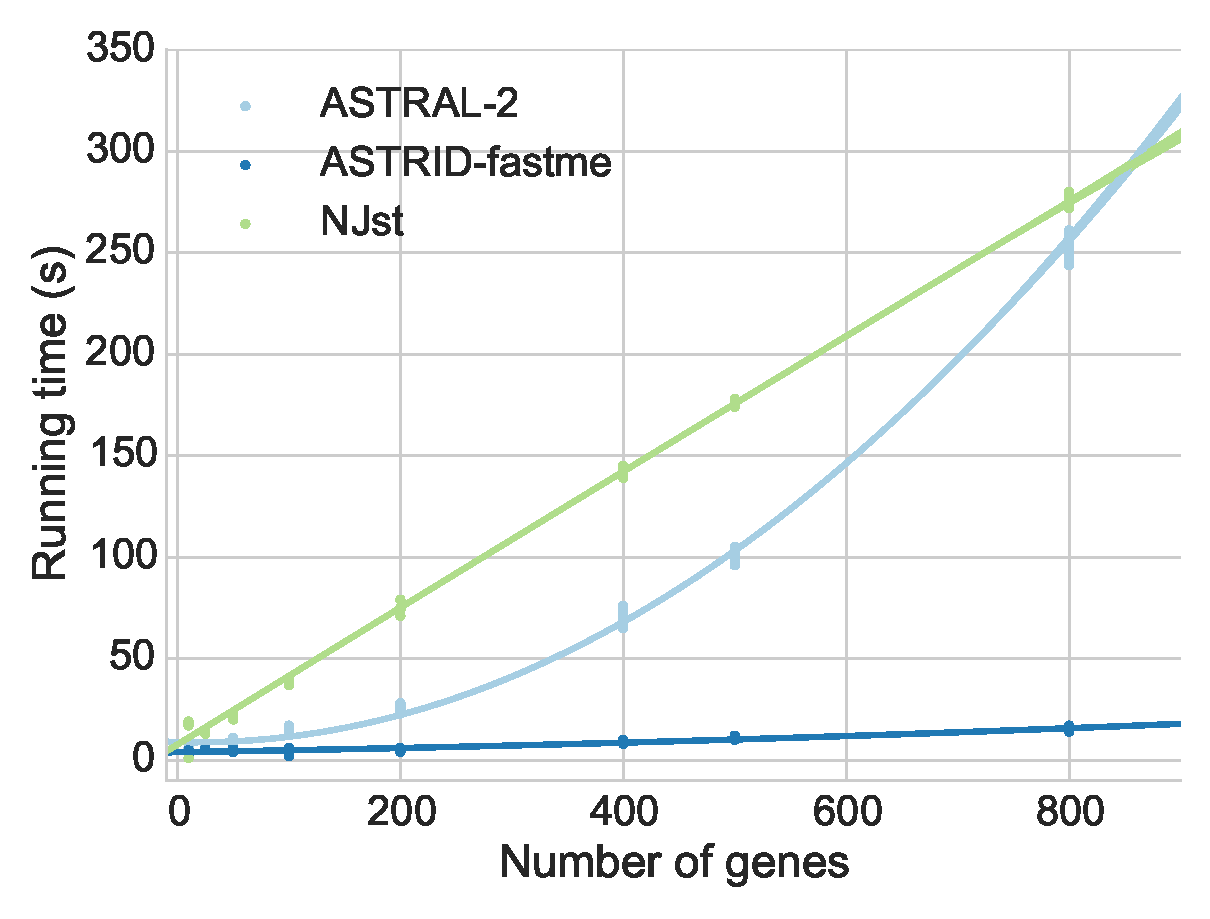
\includegraphics[width=12cm]{astrid-figs/avian-timing.eps}
  \caption[Running times for
ASTRID-FastME, ASTRAL-2, and NJst,  on avian high ILS
(1X) simulated datasets]{\textbf{Scatterplot of running times for
ASTRID-FastME, ASTRAL-2, and NJst,  on avian high ILS
(1X) simulated datasets, varying number
    of genes.} We show running time for 20 replicates of each
number of genes.    The quadratic dependence of ASTRAL-2's 
 running time is
    clearly contrasted with the linear
dependence of both ASTRID and NJst. 
    Experiments were run on a single core of a
    2.7 GHz Intel Xeon processor.}
  \label{astrid::fig:avian-timing}
\end{figure}


\begin{figure}
  \centering
  \includegraphics[width=12cm]{astrid-figs/1000-timing.eps}
  \caption[Running time 
on the ASTRAL-2 
    simulated datasets with 1000 taxa]{\textbf{Running time 
on the ASTRAL-2 
    simulated datasets with 1000 taxa (MC11), varying number of
    genes.} 
We show results for the each of the ASTRID steps -- matrix generation 
and tree estimation. We compare ASTRID used with two
ways of computing the trees: FastME and BioNJ*.
Experiments were run on a single core of a 2.7 GHz Intel Xeon processor. 
}
  \label{astrid::fig:1000-timing}
\end{figure}


\begin{figure}
  \centering
  \includegraphics[width=12cm]{astrid-figs/astral-timing.eps}
  \caption[Running time of two ASTRID methods on the ASTRAL-2 
    simulated dataset, varying number of
    taxa.]{\textbf{Running time of two ASTRID methods on the ASTRAL-2 
    simulated dataset with 500 genes, varying number of
    taxa.} We show results on a single
replicate of model conditions MC2 and 7-10 from
the ASTRAL-2 collection. Experiments were run on a single core of a 2.7 GHz Intel
    Xeon processor.}
  \label{astrid::fig:astral-timing}
\end{figure}

\section{Discussion}

A few trends are apparent upon examining the data as a whole. ASTRAL-2 
and ASTRID had, for the most part, very similar levels of accuracy,
while MP-EST was consistently less accurate.  However, there were cases 
where ASTRID and ASTRAL-2 have small but detectably different levels of
accuracy.
One intriguing trend in the data is the improvement of
ASTRAL-2 over ASTRID on high ILS datasets; see Figures~\ref{astrid::fig:mammalian-ils},
\ref{astrid::fig:astral2-ils}, \ref{astrid::fig:15taxon}, and \ref{astrid::fig:10-taxon}. 
In particular, Figures \ref{astrid::fig:mammalian-ils} and \ref{astrid::fig:astral2-ils} suggest
that increases in ILS should favor ASTRAL-2 over ASTRID. Yet, 
 ASTRID is consistently 
at least as accurate as ASTRAL-2 on the avian datasets, which
have moderate to very high levels of ILS (Fig.~\ref{astrid::fig:avian-ils}).
Thus, ILS level might have an impact on the relative accuracy of the
two methods, but it is not a determining favor.
Similarly, neither method
dominates the other based on the number of
taxa, number of genes, or amount of gene tree estimation error.
Thus, it is very difficult to characterize the conditions under which each method is
likely to have an advantage over the other.
However, even for
the cases where there are differences in accuracy, in general the differences
are fairly small. Thus, the main difference between the two methods 
is computational efficiency, where ASTRID is clearly faster. ASTRID
has the biggest running time advantage over ASTRAL-2 for large numbers
of gene trees, since ASTRID scales linearly in the number of genes
while ASTRAL scales super-linearly. This makes ASTRID an especially
good method for genome-scale datasets that have a large number of
genes.
%Pranjal


\section{Conclusion}

ASTRID is a fast and highly accurate method for species tree
estimation that is robust to high levels of ILS, and provably
statistically consistent under the multi-species coalescent model.
Like ASTRAL-2, 
 ASTRID can analyze datasets with unrooted gene trees, an
advantage that the two methods have over many other methods (e.g.,
MP-EST) that can only be run on rooted gene trees.  
ASTRID (like NJst) runs in time that is polynomial in the number of gene
trees and species, but ASTRAL-2 
 and other leading coalescent-based
methods do not have this guarantee.  Thus, ASTRID has many desirable
theoretical properties compared to existing methods.

From an empirical viewpoint, ASTRID is also extremely fast and can
analyze very large datasets in minutes, where other methods either
cannot run or take hours.  In particular, ASTRID is much faster than
ASTRAL-2, 
 especially on datasets with many genes and large numbers of
species.  ASTRID also produces more accurate trees than MP-EST and
NJst, and is competitive with ASTRAL-2 
 in terms of accuracy.

However, even better (more accurate) results might be obtained through
more extensive modifications to the ASTRID algorithm design. In
particular, the accuracy of the tree depends on the particular
distance-based method that is used. 
New distance-based phylogeny estimation methods, such as
the absolute fast converging methods 
\cite{afc,roch-science}, might provide 
improved accuracy for very large datasets with many thousands of 
species.
Another important direction is developing additional methods 
for estimating species trees from distance matrices that have good
accuracy when the distance matrix has missing data. As we saw here,
FastME produced more accurate trees than the PhyD* methods, but it
could only be applied to distance matrices without any missing data.
An extension of FastME to enable it to handle incomplete distance matrices
would also be of great interest.


This study can be expanded in several directions.
Future work should more carefully investigate the conditions 
under which ASTRID is more reliable than ASTRAL-2, and explore
performance on more biological datasets. 
This study also only investigated relatively
long sequences; a subsequent study should investigate 
the relative and absolute accuracy of ASTRID and other methods
on very short sequences, since
recombination-free loci can be very short \cite{GatesyMPE2014}.
In addition, this study only examined datasets with a single
individual per species, yet ASTRID 
(like NJst)
can be run on datasets with multiple individuals;
future work should  
evaluate the absolute and relative accuracy of ASTRID and other methods
on such data.
This study showed that  ASTRID performed well in terms of species tree topology estimation, but 
we did not explore its accuracy with respect to the estimation of 
coalescent branch lengths; future work will need to explore how well
ASTRID estimates
these numeric parameters.
Finally, it may well be that ASTRID will be most useful as
a starting tree for use within more 
computationally intensive analyses, including
Bayesian MCMC analyses (e.g., *BEAST) or
maximum likelihood analyses.



\chapter[SVDquest]{SVDquest\protect\footnotemark}\footnotetext{This chapter contains material previously published in \cite{vachaspati2018svdquest}, which was a joint work with Tandy Warnow. It has been edited slightly for brevity. PV implemented SVDquest, performed experiments, wrote the first draft, and analyzed the data. TW analyzed the data, and wrote the final draft.}
\label{chapter:svdquest}


\section{Introduction}
   

% Species tree estimation is a fundamental part of many biological
% analyses. Evolutionary processes such as incomplete lineage sorting
% \cite{maddison1997gene}, 
% gene duplication and loss
% \cite{ohno},
% and horizontal gene transfer
% \cite{woese2002evolution}
% can result in heterogeneity across the genome, so that different parts
% of the genome have different trees.  
% Much of the recent literature has focused on species tree estimation in the presence of incomplete lineage sorting (ILS),
% as - according to the multispecies coalescent model (MSC), which models gene tree heterogeneity due to ILS  -  all large-scale phylogenomic studies are expected to be affected by ILS to some extent.
% Furthermore, recent research has
% established that one of the most commonly used methods for species
% tree estimation, unpartitioned concatenation using maximum likelihood
% (CA-ML), can be statistically inconsistent under the MSC, and 
% may converge to the wrong
%  tree with probability converging to $1$ as the number of loci increases for some model species trees \cite{roch2015likelihood}!
% Simulation studies evaluating  CA-ML have  also shown model conditions where it
% can produce highly supported incorrect trees 
% in the presence of sufficiently high ILS, as well as other model conditions in which
% it performs well and may possibly be statistically consistent  (e.g., \cite{KubatkoDegnan2007,DeGiorgio2010}).



% New approaches for constructing species trees that are statistically
% consistent under the MSC have been developed
% (see  \cite{mallo-posada-2016,allman2017split} for recent reviews)
% and used in a number of biological
% analyses (e.g., \cite{Song2012,jarvis2014whole,
%   wickett2014phylotranscriptomic,Mitchell01012017,hosner2016rapid}).  
% Many of these approaches
% operate by computing gene trees on different loci and then combine
% these estimated gene trees into a species tree, and some of these
% ``summary methods" (e.g., MP-EST \cite{Liu2010a},  NJst \cite{liu2011estimating}, ASTRAL \cite{astral,mirarab2015astral,astral3}, and ASTRID  \cite{vachaspati2015astrid}) can give highly accurate results in practice in
% circumstances where CA-ML performs poorly due to high levels of gene
% tree discordance
% \cite{Liu2010a,mirarab2014evaluating,vachaspati2015astrid}.  
% Furthermore, some summary
% methods are typically very fast and can analyze large datasets.
% As a result, summary methods have become standard approaches for estimating species trees when ILS is suspected.



Proofs of statistical consistency for summary methods typically
depend on having accurate gene trees \cite{roch2015robustness}, which
is generally not expected on biological datasets.  In addition, the
proofs depend on all  sites within each locus evolving down a single tree (i.e., c-genes), and
meeting that requirement can result in very short sequences for each
locus \cite{SpringerGatesy2016}, which increases gene tree estimation
error.  
Furthermore, from an empirical standpoint, there is ample evidence that
gene tree estimation error increases the error of
species trees estimated using summary methods
\cite{huang2010sources,patel2013error,DeGiorgioDegnan2014,GatesyMPE2014,bayzid2013naive,mirarab2014evaluating,SpringerGatesy2016,Meiklejohn2016,MolloyWarnow2017},
and that CA-ML can be more accurate than even the most accurate summary methods when gene tree estimation error is sufficiently high, even in the anomaly zone (see \cite{MolloyWarnow2017} and references therein).
%\cite{Huang2010,naive-binning,statbinning,patel2013,GatesyMPE2014,%
%DeGiorgioDegnan2014,WSB,%
%SpringerGatesy-delusion,Meiklejohn2016,gatesy2016resolution}., 

The impact of gene tree estimation error on species tree estimation
has led to interest in methods that can estimate species trees without
needing to compute gene trees, and that are statistically consistent under the MSC.
One such approach is to co-estimate gene
trees and species trees; *BEAST \cite{StarBEAST} and BEST
\cite{Liu2008} are two such methods, but both are very
computationally intensive 
\cite{bayzid2013naive,bbca,knowles2009estimating,mccormack,leavitt2016resolving}.
Another type of approach estimates the tree directly from the observed site pattern frequencies using properties of the MSC,
and does not also try to estimate gene trees; examples of such methods include   
SuperMatrix Rooted Triple (SMRT) \cite{DeGiorgio2010}, SNAPP \cite{bryant2012inferring}, SVDquartets \cite{chifman2014quartet}, and METAL \cite{metal,MosselRoch2015}.
 PoMo \cite{pomo} and its improved version revPoMo \cite{revPomo} can also be considered in this category, although these methods are not established to be statistically consistent under the MSC.
%consider citing Hosner2016,rusinko-2017
These ``site-based" methods are considered
particularly suitable for  datasets generated using phylogenomic protocols such
as RADseq that produce  
  loci with very few variable sites, which makes highly accurate gene tree estimation 
unlikely
\cite{de2017phylogenomics}.

The most popular of these site-based methods is available in PAUP*
\cite{paup}
and operates as follows.  
Given a multi-locus dataset,  the loci are concatenated into a single long alignment.
Then, for each set of four species, a quartet tree for that set
is computed  using  SVDquartets.
Finally, a species tree is sought that agrees with as many of these
quartet trees as possible.
{The number of quartet trees that the species trees satisfies is called its MQSST score, where MQSST refers to the {\em Maximum Quartet Support
  Species Tree}, and
  the problem of finding the tree with the highest MQSST score is the MQSST problem.
  Because the MQSST problem } is NP-hard
\cite{jiang2001polynomial}, PAUP* uses a heuristic search  
to
seek a good solution to MQSST.  
%Pranjal - we need to provide evidence for this
This method,   which we refer to
as SVDquartets+PAUP*,  is increasingly popular in
phylogenomics studies
\cite{leache2015phylogenomics,campillo2016use,manthey2016comparison,white2016multi,leavitt2016resolving,crowl2017embracing,he2016talpid,hosner2016rapid,manthey2017relationships,moyle2016tectonic,boucher2016sequence,hime2016influence,Mitchell01012017,alexander2017genomic,de2017phylogenomics,anderson2017genotyping,white2017ultraconserved}.



We present SVDquest, a new site-based method 
for estimating species trees in the presence of ILS.
SVDquest has the same basic approach as
SVDquartets+PAUP* in that it uses
SVDquartets to estimate quartet trees,
and then combines these quartet
trees into a species tree; the difference between
SVDquest and SVDquartets+PAUP* is
the technique each uses to combine the quartet trees.
Instead of employing a heuristic search strategy,
SVDquest uses dynamic programming (an algorithm
design technique) to find a provably optimal
solution to the MQSST 
problem within a constrained search space. 
The constraints are defined by a set of {\em allowed bipartitions on
  the species set}, and we use the dynamic programming algorithm from \cite{bryant2001constructing} to find a species tree that maximizes
the quartet support score within that constrained search space.
If the search space is not constrained, then SVDquest
finds a globally optimal solution to MQSST but will run in time that is exponential in the number of species, and so be too computationally intensive to use on datasets with more than about 15-20 species. 
However, we show that we can constrain the search
space so that the algorithm runs in polynomial time and
finds very good solutions to its optimization problem.
 Furthermore, by
selecting the bipartitions appropriately, the new method, which we
refer to as SVDquest*, is {\em guaranteed} to satisfy at least as many
quartet trees computed by SVDquartets as SVDquartets+PAUP*.



We present results from an extensive performance study using both simulated and biological datasets.
We find that SVDquest* finds better MQSST scores than SVDquartets+PAUP* under most
conditions, particularly under higher levels of ILS and gene tree
estimation error.  
We compare SVDquest* to a set of leading species tree estimation 
methods. We include two summary methods
ASTRAL \cite{ASTRAL,mirarab2015astral} and
ASTRID \cite{vachaspati2015astrid}, because these two methods have been shown to
have high accuracy under a wide range of model conditions and are both
statistically consistent under the MSC {(again, under the assumption that each is given true gene trees)}.
We also include  CA-ML (using RAxML), since (as noted earlier)  trees computed using CA-ML are often at least as accurate as
trees computed using summary methods. 
We do not include any of the co-estimation methods, as they are too computationally intensive to use
on the datasets we explore.

The relative performance between these methods depends on the
model condition (and in particular on the amount of gene tree estimation 
error), but SVDquest*  has dramatic improvements over the summary
methods under conditions with high
average gene tree estimation error and many genes.  
CA-ML has the best
accuracy of all methods under conditions with low to moderate ILS, but
the coalescent-based methods outperform CA-ML when ILS is sufficiently
high. 

Finally, we also show that returning the strict consensus of the optimal trees
computed by SVDquest* provides further improvements in topological accuracy. 
Thus, SVDquest* is a new method with improved accuracy
compared to existing coalescent-based species tree methods under a
range of realistic model conditions.


   

\section{Materials \& Methods}

\subsection{SVDquest}

The input to SVDquest is a set of sequence alignments (one alignment
for each locus).  
Phase 1 of SVDquest uses the SVDquartets implementation in PAUP* to compute a set of quartet trees
and Phase 2 combines these quartet trees into a species tree on the
full set of species.  
Thus, SVDquest is identical to SVDquartets+PAUP* in Phase 1, but differs from SVDquartets+PAUP* in Phase 2.
{
Specifically, SVDquest uses dynamic programming to find an optimal solution to the MQSST problem within a constrained search space, similar to how ASTRAL and FastRFS \cite{fastrfs} (a method for the Robinson-Foulds Supertree problem) find optimal trees for their optimization problems within constrained search spaces.
Furthermore, since there can be more than one optimal tree for the MQSST problem, we}
also consider an optional Phase 3, in which a consensus tree is computed on the optimal trees found in Phase 2 using SIESTA \cite{vachaspati2017enhancing}, a method that
can be used with dynamic programming methods (such as SVDquest) that solve constrained
optimization problems.
 As shown in \cite{vachaspati2017enhancing}, the use of  SIESTA with ASTRAL and FastRFS   to compute the strict consensus tree typically results in an improvement in overall topological accuracy, 
 suggesting that SIESTA might also improve SVDquest*.





\paragraph{Phase 1: computing the set $Q$ of quartet trees. }
Phase 1 (the quartet tree estimation phase) computes 
an unrooted binary tree for every set  of four species. 
For each set of four species, we use SVDquartets as implemented in PAUP* to select the best
of the three possible quartet trees, and we refer to the set of all
quartet trees computed in this way by $Q$.  
In some cases, SVDquartets
will not return a tree on a set of four species because the scores are
too close (e.g., this can happen when there are too few variable
sites).


\paragraph{Phase 2: computing an optimal species tree from using 
$Q$. }
Phase 2 (the species tree estimation phase) uses the quartet trees
computed in Phase 1, and attempts to find an optimal solution to the MQSST problem.  
Since MQSST is NP-hard, algorithms for finding the globally optimal solution are not scalable. 
Hence, SVDquest typically operates in a mode
where instead of searching for a globally optimal tree, it finds an optimal tree within a constrained search space.

SVDquest has three modes: {\em unconstrained, constrained-basic}, and
{\em constrained-enhanced}.  The {\em unconstrained} mode does not
constrain the search space at all and hence is the most
computationally intensive; it can only be used when the number of
species is small enough (up to 15-20 taxa).  In the two
constrained modes, the search space is defined by a set $X$ of
bipartitions on the species set, and the constraint is that the output
species tree {\em must} draw its bipartitions from $X$.  
Therefore, if $X$ is all possible bipartitions on the species set then
there is no constraint on the set of species trees that can be
returned; otherwise, there is a reduction in the set of species trees
that can be considered during the search for the best tree.

To compute the basic set $X$ of allowed bipartitions, SVDquest uses
the following protocol.  First, it computes maximum likelihood trees
on every gene; then, it runs a subroutine in ASTRAL-II
\cite{mirarab2015astral} to compute a set $X$ of bipartitions that is
guaranteed to include all the bipartitions from the input gene trees.
The enhanced set of allowed bipartitions is computed by adding
bipartitions to $X$. For example, we can add the bipartitions in the
SVDquartets+PAUP* tree to $X$; we refer to this \emph{constrained-enhanced}
variant as SVDquest*.  Since SVDquest exactly solves the MQSST
optimization problem within the constrained search space, the
SVDquest* tree is {\em guaranteed} to have a MQSST score that is at
least as good as the SVDquartets+PAUP* tree's MQSST score.

{
\paragraph{Phase 3: Returning the strict consensus of the set of optimal trees computed in Phase 2.}
As noted, there can be more than one species tree that has an optimal MQSST score within the constrained space.
Hence we provide an optional Phase 3 in which we use SIESTA to compute the strict consensus of all the trees in that set.
}

{
\paragraph{Comparison between SVDquartets+PAUP* and SVDquest variants. }
}

SVDquest  and SVDquartets+PAUP* are  techniques that compute a set $Q$ of quartet trees using SVDquartets and then attempt to find a species tree that satisfies the maximum number of quartet trees in $Q$.  
The key difference between these methods is how each it solves the MQSST problem. 
SVDquest and its variants use a polynomial time dynamic programming algorithm from
\cite{bryant2001constructing} to {provably} solve MQSST within a constrained search space;
in contrast, {PAUP* uses other techniques to attempt to solve MQSST that do not provide guarantees of optimality within any constrained search space, but have the benefit of  not being explicitly constrained to a subset of the search space.}



\subsection{Datasets}

We explored performance on 10-, 15-, and 50-taxon simulated datasets. 
We also analyzed a  mammalian biological dataset  with 37 species that was
first studied in \cite{Song2012}, and later used to compare coalescent-based methods
\cite{mirarab2014astral,SpringerGatesy2016,bayzid2013naive}. 
The mammalian dataset originally included 447 loci, but 21 of these
had mislabeled sequences and two were clear outliers \cite{ASTRAL},
so we excluded them from our analysis. 
This left 424 loci and a total of 1,338,678 sites in the
concatenated alignment.  
We obtained the alignments and RAxML gene trees from \cite{Song2012}, and we obtained the CA-ML tree on the 424 loci from \cite{ASTRAL}.
The average bootstrap support on the gene trees was $71\%$.  The main questions are the
positions of two groups: \emph{Chiroptera} and \emph{Scandentia}.



% \begin{table}
%   \centering
%   \begin{tabular}{|r|r|r|r|r|}
%     \hline
%     &\# Taxa&\# Loci&\# Sites&Avg. locus length\\
%     \hline
%     Lichen     & 31 &  100      &    92,670            & 306   \\
%     Mammalian   & 37 &  424      & 1,338,678            & 3,157 \\
%     Landfowl   & 91 & 140 &    75,998 & 542\\
%     True Frog  & 94 &   14      &     7,250            & 517   \\
    
%     \hline
%   \end{tabular}
%   \caption{Descriptions of  the biological datasets studied in this paper.
%     }\label{svdquest::bio-statistics}
% \end{table}


%\subsubsection{Simulation Process}

The simulated datasets were derived from prior publications, described
individually below.  Each dataset has model gene trees that evolve
down model species trees under the multi-species coalescent, and
indel-free sequence alignments evolved down those gene trees under
standard site evolution models.  Each gene is a proper c-gene (i.e.,
there is no recombination within any gene), and unless specified
otherwise, the strict molecular clock assumption is not enforced.  
In some cases, we combined sequence data from different genes together (to simulate  failure to detect recombination)  by concatenating sequences
simulated on gene trees with different topologies; this produces a set of ``supergene" datasets.

Statistics for the simulated c-gene datasets are presented in Table
\ref{svdquest::sim_summary}. To characterize the level of ILS, we use the AD value,
which is the average normalized Robinson-Foulds (RF) distance
\cite{robinson1981comparison} between model gene trees and model
species trees (i.e., the percentage of the non-trivial bipartitions in
the true gene tree that do not appear in the true species tree).  We
also report gene tree estimation error (GTEE), which is the average
normalized RF distance between model gene trees
and estimated gene trees.


The 50-taxon datasets were simulated with SimPhy \cite{SimPhy} and
were originally presented in \cite{mirarab2015astral}. These datasets
have 50 taxa, 1000 loci, and 300-1500 sites per locus. The original
versions of these datasets have 200 taxa, but 150 taxa have been
randomly removed from each replicate to reduce the time and memory
requirements of the analysis. This dataset contains three model
conditions with three different ILS levels of 13\%, 33\%, and 72\%
AD. Loci were originally of variable length, but we reduced the sequence lengths for these experiments to 25, 50, 100, and 300 sites.
These datasets have a speciation rate of $10^{-6}$, resulting in speciation close to the tips of the model trees (i.e., recent divergence). 
Sequences evolved with a GTR+Gamma model and no molecular
clock.

{
There were 26 model conditions (all with very high ILS) on which SVDquartets+PAUP* and SVDquest failed to return a tree. In these cases, PAUP* reported that there were ``No informative quartets found", and examining the sequences showed that there were very parsimony-informative sites. 
Hence, we report results only on those replicates for which all methods completed, 
a number that varies from 48 to 50 for each model condition.
See Section \ref{svdquartets-failure} for additional details.
}



The 15-taxon simulated datasets (from \cite{bayzid2015weighted}) have
very high ILS (82\% AD), and have 1000 loci with 1000 sites evolved
with a strict molecular clock using a GTR+Gamma model (i.e., the gene trees are
ultrametric).  
Model species
trees all have the same ``caterpillar'' topology, and gene trees obey
a strict molecular clock. We used 10, 100, and 1000 sites per locus,
with an average of $65\%$, $53\%$, and $18\%$ GTEE, respectively. 
Each
model condition has 10 replicates, and all of them completed
successfully with all methods.



The 10-taxon simulated datasets (also from \cite{bayzid2015weighted})
have two ILS levels (43\% and 84\% AD). % and no molecular clock.
These datasets have 200 loci with 10, 50 and 100 sites per
locus, and GTEE levels between 40\% and 75\%.
Species trees were randomly generated under a Yule process,
gene trees are not ultrametric, and sequence data evolved under a
GTR+Gamma model. 
Each model condition has 20 replicates; however, as with the 50-taxon datasets, some replicates had  too few parsimony-informative sites, so that SVDquartets failed to compute any
quartet trees. This occurred for 10 replicates of each model condition (combination of ILS level, number of genes, gene sequence length), and we
report results for the other 10 replicates of each model condition.



\begin{table}
  \centering
  \begin{tabular}{|r|r|r|r|}
    \hline
    Number of  taxa&50&15&10\\
    \hline
    Number of loci&50, 100, 500, 1000 & 50, 100, 1000& 25, 50, 200 \\   
    Locus length & 25, 50, 100, 300 & 10, 100, 300 & 10, 50, 100\\   
    GTEE &15\%-100\% & 15\%-72\% & 40\%-75\% \\    \hline
   AD\% (ILS) & 13\%, 33\%, 72\% & 82\% & 43\%, 84\% \\    \hline
  Number of replicates & 40-50 & 10 & 10 \\    \hline
    Strict molecular clock? & No & Yes & No \\
    \hline
  \end{tabular}
  \caption[Summary of simulated datasets for SVDquest study]{Summary of simulated datasets. GTEE is gene tree estimation
    error (i.e.,  the 
   average normalized Robinson-Foulds distance between the 
     estimated and model gene
    trees).  AD\% measures the average normalized Robinson-Foulds distance 
    between
    the model gene trees and the model species tree, and is due only to 
    ILS.  }\label{svdquest::sim_summary}
\end{table}

\subsection{Species tree methods for comparison}

We compared SVDquest* to ASTRAL v4.10.2 \cite{mirarab2015astral},
ASTRID v1.4 \cite{vachaspati2015astrid}, SVDquartets+PAUP* as implemented in
PAUP* v4.0a151 \cite{paup}, and unpartitioned concatenated maximum
likelihood (CA-ML) under a GTR-GAMMA model using RAxML v8.2.6
\cite{Stamatakis2006}. The same version of RAxML was used to estimate trees on gene sequence alignments and supergene sequence alignments
under a GTR-GAMMA model. 
We ran the Windows version of PAUP* using WINE v1.6.2 due to its improved
numerical routines compared to the Linux version. 
Exact commands for all methods are
supplied in the appendix.

\subsection{Evaluation criteria}
On the simulated datasets we  use Dendropy \cite{dendropy} to evaluate estimated trees  for topological accuracy.
All model species trees are binary (i.e.,  fully resolved), but some of the estimated
species trees are not binary; hence, 
we report  the average of the false positive and false negative
rates; this is identical to normalized Robinson-Foulds (RF) error rates \cite{robinson1981comparison} when the estimated trees are binary. 

On the mammalian biological dataset, we evaluated the estimated species trees using established clades, taking branch support  into account.
For branch support on trees computed using the summary methods and CA-ML, we used the local  posterior probability branch support technique  \cite{sayyari2016fast}  in ASTRAL, which is based on the initial set of estimated gene trees and has been shown to produce better estimates of the probability of a branch being accurate than multi-locus bootstrapping  \cite{sayyari2016fast}.
Branch support of species trees computed using site-based methods such as SVDquartets+PAUP* or CA-ML is  commonly performed using
non-parametric bootstrapping, but  this approach is  computationally intensive because  it requires the 
calculation of species trees for all the bootstrap replicates. 
For this reason, we used a modified non-parametric bootstrap support technique described below (with 100 bootstrap replicates) to produce estimates of the branch support for the SVDquest* tree, and
we compare the branch support we obtained using this modified non-parametric bootstrapping technique to the support we receive using the usual non-parametric bootstrapping
technique.
The modification to non-parametric bootstrapping that we use is very simple, and provides an approximation to the branch support that would be obtained using full non-parametric bootstrapping.
We compute the constraint set $X$ of bipartitions  using  the original dataset (i.e., not bootstrapped).  Then, for each of the 100 bootstrap replicates,  we run 
SVDquartets  to compute the quartet trees, and we
 run SVDquest on the quartet trees computed by SVDquartets, using the constraint set $X$.
In every other respect, the estimation of branch support we use follows the same protocol as with the usual non-parametric boostrapping procedure.
Note that this approach has the benefit  that for every bootstrap replicate the quartet trees are based correctly on SVDquartets,  and only differs from full non-parametric bootstrapping in how the search space is constrained.
Hence, this branch support technique  does not affect the MQSST score of any returned tree, and only constrains which trees are considered permitted solutions. 

\subsection{Experiments}

\paragraph{Experiment 1: Comparing SVDquest* and SVDquartets+PAUP* on simulated c-genes with respect to  MQSST scores. }

The goal of this experiment is to determine whether SVDquest* finds
better MQSST scores than SVDquartets+PAUP*. We tested both methods
on simulated and biological datasets and reported MQSST
criterion scores.


\paragraph{Experiment 2: Comparing coalescent-based species tree
  estimation methods on simulated c-genes with respect to tree topology. }


In the second experiment, we evaluated SVDquest*, SVDquartets+PAUP*, ASTRAL, and ASTRID, with respect to tree topology accuracy on a wide range of simulated
datasets where  all genes are c-genes (i.e., for each gene, all the sites evolve down a common tree topology).


\paragraph{Experiment 3: Comparison of coalescent-based species tree methods on multi-locus supergene datasets. }

In this experiment, we explored  SVDquest*, SVDquartets+PAUP*, ASTRAL,  and ASTRID  on   multi-locus datasets where the c-genes are randomly combined into supergenes (with the same number of c-genes), so that the assumption that 
all the sites in a given locus evolve down the same tree is violated.
This experiment
is motivated by the real-world challenge  of failing to detect
recombination events within gene sequence alignments.  
We estimated ML trees on these supergene
alignments, and then used these ``supergene trees'' as the input for ASTRAL and ASTRID.
Since SVDquartets computes quartet trees using all the sites in the concatenated alignment, this does not impact SVDquartets; it also
 does not change MQSST scores for any estimated species tree, as these are based on the  quartet trees computed using SVDquartets. 
 Hence, the use of supergenes does not impact SVDquartets+PAUP*.
 However, the use of supergenes instead of genes impacts summary methods, 
since  the supergene trees will not be equal to the gene trees.  It also affects SVDquest and SVDquest*, since it can change the constraint space that it computes using ASTRAL. 

\paragraph{Experiment 4: Comparison of coalescent-based methods to CA-ML on simulated datasets. }

In this experiment, we compared CA-ML to SVDquest*, ASTRAL, and ASTRID
on all simulated datasets with respect to the normalized
Robinson-Foulds  topological error rates.

\paragraph{Experiment 5: Comparison of coalescent-based methods on a mammalian biological dataset. }

We compare the SVDquest* tree 
on the mammalian biological
dataset to trees computed using SVDquartets+PAUP*,
ASTRAL, and ASTRID (all three trees
computed by us), as well as to a concatenation
analysis (obtained from \cite{ASTRAL}),  with respect to
branch support for established and proposed clades.



\paragraph{Experiment 6: Running time. }
We explore running time for SVDquartets+PAUP*, SVDquest, SVDquest*, and ASTRAL
on the 37-taxon mammalian biological dataset.




\section{Results}


\subsection{Results for Experiment 1}


Experiment 1 compares SVDquest, SVDquest* and SVDquartets+PAUP* with respect to  the MQSST scores they find.
Although SVDquest does not always find better scores than SVDquartets+PAUP*,
%{(see Supplementary Materials, Table S1)}, 
by design SVDquest* is guaranteed to find scores that are at least as large as those
found by SVDquartets+PAUP*.
In this section, we report the number of cases where SVDquest* finds a better score than SVDquartets+PAUP* and
the number of cases where they have the same score; we also
show the distribution of GTEE on the various datasets.


On the 50-taxon data, shown in Figure \ref{svdquest::fig:exp1_50}, a few basic
trends are clear. 
SVDquest* has a much greater advantage over SVDquartets+PAUP* at
higher ILS levels, almost always finding better scores on the highest
ILS model condition. SVDquest* also has a larger advantage when there
are 50 or 100 genes, as opposed to 500 or 1000 genes. 
Generally, the advantage of 
SVDquest*' over SVDquartets+PAUP* improves as gene tree estimation error (GTEE)
increases, until the very highest GTEE rates where
the advantage starts to fall. 
See also figures \ref{fig:s1}-\ref{fig:s3} for  histograms of differences in MQSST scores between SVDquartets+PAUP* and SVDquest* on these datasets.

Results on the 15-taxon data (AD=82\%), shown in Figure \ref{svdquest::fig:exp1_15}, also show
that SVDquest* has a bigger advantage when there are fewer genes in
the dataset. When there are 1000 genes, SVDquest* and SVDquartets+PAUP* almost
always find trees with the same score, but SVDquest* frequently finds
better trees when there are 50 or 100 genes. 
The impact of GTEE on the advantage with respect to MQSST score is less obvious on 50- and 100-gene datasets, but this
may be because 
the range of GTEE is less than in the 50-taxon data.
%See also Supplementary Materials ... for the histogram of differences in MQSST scores between SVDquartets+PAUP* and SVDquest* on these datasets.

The results on the 10-taxon data, shown in Figure \ref{svdquest::fig:exp1_10},
once again show that increasing the ILS level or decreasing
the number of genes increases the 
frequency with which SVDquest finds a tree with a better MQSST
score than SVDquartets+PAUP*.
 Like the 15-taxon datasets, which have
similar levels of GTEE,  the relationship
between GTEE and the relative performance of the two methods on these
datasets is less clear than on the 50-taxon datasets.
%See also Supplementary Materials ... for the histogram of differences in MQSST scores between SVDquartets+PAUP* and SVDquest* on these datasets.



\begin{figure}
  \centering
	  \includegraphics[width=\textwidth]{svdquest-figs/svdquestplus_vs_paup_better_score.pdf}
  \caption[Comparison of SVDquest* and SVDquartets+PAUP* with respect to MQSST scores on 50-taxon simulated data]{Results for Experiment 1 on 50-taxon data, showing how
    often SVDquest* finds better MQSST scores than SVDquartets+PAUP*. Pink
    sections of bars represent replicates where SVDquest* finds a
    better scoring tree; blue sections represent replicates where both
    methods find the same scoring tree. It is impossible for SVDquartets+PAUP* to
    find a better scoring tree than SVDquest*. Total heights of bars
    represent distribution of  gene tree estimation error (maximum possible value is 1.0) in
    datasets. {Each subfigure shows results for 200 replicates, with the exception of the AD=72\% datasets, which have 195-200 replicates each}.}\label{svdquest::fig:exp1_50}

\end{figure}


\begin{figure}
  \centering
  \includegraphics[width=\textwidth]{svdquest-figs/svdquestplus_vs_paup_better_score_15tax.pdf}
  \caption[Comparison of SVDquest* and SVDquartets+PAUP* with respect to MQSST scores on 15-taxon high ILS simulated data]{Results for Experiment 1 on 15-taxon data with 82\% AD
   (high ILS),
    showing how often SVDquest* finds a better scoring tree than
    SVDquartets+PAUP*. Pink sections of bars represent replicates where SVDquest*
    finds a better scoring tree; blue sections represent replicates
    where both methods find the same scoring tree. It is impossible for SVDquartets+PAUP* to
    find a better scoring tree than SVDquest*.  Total heights of
    bars represent distribution of gene tree estimation error (maximum possible value is 1.0) in
    datasets. Each subfigure shows results for 30 replicates.
    }\label{svdquest::fig:exp1_15}
\end{figure}

\begin{figure}
  \centering
  \includegraphics[width=\textwidth]{svdquest-figs/svdquestplus_vs_paup_better_score_10tax.pdf}
\caption[Comparison of SVDquest* and SVDquartets+PAUP* with respect to MQSST scores on 10-taxon simulated data]{Results for Experiment 1 on 10-taxon data, showing how
    often SVDquest* finds a better scoring tree than SVDquartets+PAUP*. Pink
    sections of bars represent replicates where SVDquest* finds a
    better scoring tree; blue sections represent replicates where both
    methods find the same scoring tree. It is impossible for SVDquartets+PAUP* to
    find a better scoring tree than SVDquest*. Total heights of bars
    represent distribution of gene tree estimation error (maximum possible value is 1.0) in the
    datasets.  
      Each subfigure shows results for 30 replicates.   
    }\label{svdquest::fig:exp1_10}
\end{figure}


\clearpage
\subsection{Results for Experiment 2}
%rfdistance

Experiment 2 evaluates  %SVDquest* and 
SVDquest*-strict (i.e., 
the strict consensus of all optimal trees found by SVDquest*, computed using SIESTA) 
in terms of topological accuracy 
on simulated c-gene datasets, and also compares it to ASTRID, ASTRAL, and SVDquartets+PAUP.  
{The comparison between SVDquest*-strict and SVDquartets+PAUP* on the 50-taxon datasets (Figures \ref{fig:s4}-\ref{fig:s7}) shows that although SVDquest*-strict and SVDquartets+PAUP* have similar accuracy, SVDquartets+PAUP* has an advantage over SVDquartets+PAUP*. }

%By varying the level of ILS, GTEE, number of taxa, and number
%of genes, we also see how these dataset properties impact the relative
%and absolute performance of these species tree estimation methods.


%Our first part of this experiment compares  SVDquest*   and SVDquest*-strict.
%%SVDquest* tended to be more accurate than SVDquest (i.e., when it
%%differed from SVDquest, the trees were typically more accurate), suggesting that
%%improving the MQSST scores tended to improve topological accuracy %{(see Supplementary Materials, Figures XX-YY}. 
%Furthermore,  when there was more than one optimal tree, then  the strict consensus %tree of the optimal trees also tended
%to have better  topological accuracy {(see Supplementary Materials, Figures XX-YY)}. 
%Hence, in our remaining comparisons we report accuracy for SVDquest*-strict. 


{A comparison between SVDquest*-strict, ASTRAL, and ASTRID} on the 50-taxon datasets with 500 genes is shown in Figure \ref{svdquest::fig:exp2_50}
({see Figure \ref{fig:s8} for other numbers of genes}).
These datasets do
not evolve under a strict molecular clock and vary in ILS levels
(reflected in AD percentages), GTEE, and number of genes.  ASTRAL and
ASTRID have similar accuracy levels under most conditions.  At low
levels of GTEE, all methods are fairly accurate.  With high GTEE,
SVDquest*-strict is much more accurate than ASTRAL and ASTRID. 
At high levels
of ILS and low GTEE, ASTRAL and ASTRID are more accurate than
SVDquest*-strict.  Across all model conditions, the crossover point where
SVDquest*-strict becomes more accurate is approximately 50\% GTEE. 
SVDquest*-strict
also has a bigger advantage over ASTRAL and ASTRID when ILS levels are
lower and there are more genes. 
In the most extreme case with close to
100\% GTEE, 13\% AD, and 1000 genes
{(see Figure \ref{fig:s8})},
ASTRAL  has approximately 75\% estimation error while
SVDquest*-strict has only 10\% estimation error. 

Figure \ref{svdquest::fig:exp2_15} shows results on the 15-taxon datasets (AD=82\%), which
evolve under a strict molecular clock. 
ASTRAL is the most accurate method in all cases. 
The comparison between SVDquest*-strict and ASTRID shows that SVDquest*-strict
has an advantage for the model conditions with largest number of genes (1000) and highest GTEE (40-60\%),
ASTRID has an advantage for the model conditions with fewest genes (50-100) and lowest GTEE (0-20\%), and
otherwise the two methods have similar species
tree estimation error. 
However, this dataset has a relatively limited
range of gene tree error - no replicate has greater than 60\% average
GTEE, which is the model condition where we would expect the best
performance from SVDquest*-strict. 

Results on the 10-taxon data (which do not evolve under a strict
molecular clock) are shown in Figure \ref{svdquest::fig:exp2_10}.  All three
methods have similar levels of accuracy under most conditions.
However, ASTRAL frequently returns slightly more topologically
accurate trees than the other two methods, and ASTRAL and ASTRID are
somewhat more accurate than SVDquest*-strict when there is low GTEE. Like the
15-taxon data, this model condition has no replicates with greater than
60\% average GTEE.

\clearpage

\begin{figure}
  \centering
  \includegraphics[width=\textwidth]{svdquest-figs/coalescent_rfdists_500.pdf}
  \caption[Species tree topological error rates for 50-taxon simulated data]{Species tree topological error rates (maximum possible is 1.0) for 50-taxon simulated data, as a function of percent
    gene tree estimation error (maximum possible is 1.0); {the first two figures show results for 200 replicates and the last figure shows results for 198 replicates.} 
    Error bars show standard
    error.    
    }\label{svdquest::fig:exp2_50}
    \end{figure}


\begin{figure}
  \centering
  \includegraphics[width=\textwidth]{svdquest-figs/coalescent_rfdists_15tax.pdf}
  \caption[Species tree topological error rates for 15-taxon simulated data]{Species tree topological  error rates (maximum possible is 1.0) 
  for 15-taxon simulated data (AD=82\%), as a
    function of gene tree estimation error (maximum possible is 1.0); each subfigure shows results on 30 replicates. Error bars show standard
    error.   
    }
    \label{svdquest::fig:exp2_15}\end{figure}

\begin{figure}
  \centering
  \includegraphics[width=0.8\textwidth]{svdquest-figs/coalescent_rfdists_10tax.pdf}
\caption[Species tree topological error rates for 10-taxon simulated data]{Species tree topological error rates (maximum possible is 1.0) for 10-taxon simulated data, as a
    function of gene tree estimation error (maximum possible is 1.0); each subfigure shows results for 30 replicates. Error bars show standard
    error. 
}
    \label{svdquest::fig:exp2_10}
\end{figure}


\clearpage
\subsection{Results for Experiment 3}

Experiment 3 compares SVDquest*-strict to  ASTRAL, ASTRID, and SVDquartets+PAUP* on supergene datasets (i.e.,  when loci are not
recombination-free). 
We report both MQSST scores and topological accuracy.


The comparison between SVDquartets+PAUP* and SVDquest*-strict shows that
SVDquest*-strict typically matches or improves on SVDquartets+PAUP* with respect to
topological accuracy  {(Figures \ref{fig:s9}-\ref{fig:s11})}. 
In fact, the advantage of using SVDquest*-strict over SVDquartets+PAUP* is greater
on the supergene datasets than on c-gene datasets.
In what follows, we compare SVDquest*-strict to ASTRAL and ASTRID.


Results on the 50-taxon datasets are shown 
in Figure \ref{svdquest::binned_50}. 
The recombination-free loci have only 25 sites; all other
lengths indicate supergenes obtained by combining c-genes.
On all the model
conditions with 25-site loci,
SVDquest*-strict has a substantial advantage over ASTRID and ASTRAL. 
On the
lowest ILS model condition, SVDquest*-strict retains the same accuracy as the
c-genes are combined into supergenes. 
However, as the number of c-genes per supergene increases, ASTRAL and ASTRID become
more accurate,  eventually equaling or improving over SVDquest*-strict. 
For example, on the 33\% AD  model condition, SVDquest*-strict has an
advantage when the supergenes have at most two c-genes, but  then only
ties with ASTRAL and ASTRID when there are 
more c-genes per supergene.  
On the 72\% AD 
model condition, SVDquest*-strict retains an advantage regardless of the
number of c-genes per supergene, but the advantage decreases with the length
of the supergene. 

Results on the 15-taxon datasets are seen in Figure \ref{svdquest::binned_15}.
The c-genes have only 10 sites; all other lengths
indicate supergenes obtained by binning together different c-genes.
At the longest supergenes with 1000 sites (each composed of
100 recombination-free loci), ASTRAL and ASTRID find more accurate
trees than SVDquest*-strict, but at lower levels of binning, SVDquest*-strict finds
trees that are more accurate than ASTRID but less accurate than
ASTRAL. ASTRAL finds slightly more accurate trees when the loci are
recombination-free, while ASTRID improves substantially with increased
binning, especially when there are 1000 loci.  The impact of binning
on SVDquest*-strict is minimal.

Relative performance on the 10-taxon data, shown
in Figure \ref{svdquest::binned_10}, is similar to the
15-taxon data. ASTRAL typically becomes less accurate at higher levels
of binning, while SVDquest*-strict is  relatively unaffected, and ASTRID
sometimes improves. These trends are more evident at the 84\% AD
level; at the 43\% AD level, there is relatively little change with
increased binning.

\clearpage
\begin{figure}
  \centering
  \includegraphics[width=0.9\textwidth]{svdquest-figs/binned_rfdists_nocaml_no1000.pdf}
  \caption[Species tree topological error rates for 50-taxon simulated data with supergenes]{Species tree error rates (maximum possible is 1.0) on 50-taxon simulated data using 
    supergenes (concatenations of c-genes)
    that may not be recombination-free. Error bars represent standard error of the mean. The c-genes in this experiment are 25 sites long, and multiple loci were
    concatenated to form supergenes. Thus, the 
    25-site genes have sites coming from one c-gene, the 50-site genes have
    sites coming from two c-genes, and the 100-site genes have sites coming
    from four c-genes. Each data point in a particular subfigure represents
    an analysis on the same number of sites. 
    {
    Each data point corresponds to an average over 50 replicates, except for the AD=72\% 25-site 50-gene data point, which corresponds to 48 replicates, and 9 other AD=72\%  data points, each of which corresponds to 49 replicates.}
  }\label{svdquest::binned_50}
\end{figure}


\begin{figure}
  \centering
  \includegraphics[width=\textwidth]{svdquest-figs/binned_rfdists_nocaml_15tax.pdf}
  \caption[Species tree topological error rates for 15-taxon simulated data with supergenes]{Species tree error rates (maximum possible is 1.0) on 15-taxon simulated data (AD=82\%) for three different numbers of c-genes, then binned into 
    supergenes (concatenations of c-genes); results shown are averaged over 10 replicates with error bars
    representing standard error of the mean.
    The c-genes in this experiment
    have 10 sites, so that longer loci are supergenes.  Each data point in a particular
    subfigure represents an analysis on the same total number of sites. 
    }\label{svdquest::binned_15}
\end{figure}



\begin{figure}
  \centering
  \includegraphics[width=\textwidth]{svdquest-figs/binned_rfdists_nocaml_10tax.pdf}
  \caption[Species tree topological error rates for 10-taxon simulated data with supergenes]{Species tree error rates (maximum possible is 1.0) on 10-taxon simulated data using
    supergenes (concatenations of c-genes), averaged over 10 replicates; error bars
    represent standard error of the mean. The c-genes in this experiment
    have 10 sites, and longer sequences are supergenes.
    Each data point in a particular subfigure
    represents an analysis on the same number of sites. 
    }\label{svdquest::binned_10}
\end{figure}


\clearpage

\subsection{Results for Experiment 4}

Experiment 4 compares coalescent-based methods to unpartitioned
concatenation using RAxML (i.e., CA-ML) on simulated datasets.  On the 50-taxon data, seen in
Figure \ref{svdquest::fig:exp3_50} for 500 gene datasets
{(see Figure \ref{fig:s8} for other numbers of genes)},
CA-ML and SVDquest*-strict tend to perform similarly, and better than ASTRID
and ASTRAL when GTEE is greater than 60\%.  
On the lower ILS (13\% AD)
condition, CA-ML is somewhat more accurate than SVDquest*-strict when there
are fewer genes  {(Figure \ref{fig:s8})}, but this advantage is
reduced for 500 or 1000 genes. At the highest ILS level, CA-ML is
actually less accurate than SVDquest*-strict when there are few genes and low
GTEE, but both of these methods are less accurate than ASTRAL and
ASTRID.

On the 15-taxon data (AD=82\%), shown in Figure \ref{svdquest::fig:exp3_15}, 
ASTRAL is always the
most accurate method. ASTRID performs worse than CA-ML and
SVDquest*-strict when there are 50 or 100 genes. With 1000 genes, all methods
perform well, but ASTRAL and ASTRID slightly outperform CA-ML and
SVDquest*-strict. 

On the 10-taxon data, shown in Figure \ref{svdquest::fig:exp3_10}, CA-ML is
typically the best method on the 43\% AD  data. 
CA-ML slightly
outperforms the other methods except when there are 50 genes and low
GTEE, in which case ASTRAL and ASTRID perform slightly better. On the
84\% AD  data, SVDquest*-strict and CA-ML are the worst performing
methods, and ASTRAL is typically the best method.

We calculated the rank correlation coefficient between
the MQSST scores and topological errors for PAUP* and SVDquest* in
order to determine whether a better MQSST score was correlated with a topologically
more accurate tree. 
We found that there was a statistically
significant correlation ($P < 0.05$) with a Spearman rank correlation coefficient of $\rho = 0.32$ for the 50-taxon datasets.


\subsubsection{Results for Experiment 5}



We compared SVDquest* to  SVDquartets+PAUP*, CA-ML, ASTRAL, and ASTRID trees
on the mammalian biological dataset.
CA-ML, ASTRAL, and ASTRID all return the same tree, 
which recovers the major accepted mammalian clades and
the relationships between them, but SVDquest* 
 {returns a  single tree that is different from the tree found
 by the other methods.}
 {See Figure \ref{svdquest::fig:mammalian-svdquestplus} for the SVDquest* tree with bootstrap branch support, and Figure \ref{fig:s12} for the ASTRAL/ASTRID/CA-ML tree with ASTRAL branch support. }
 The SVDquest* tree has very high bootstrap branch support on
nearly all the edges (100\% support on all but four edges and 99\% support on one edge), and the ASTRAL/CA-ML/ASTRID tree has over 90\% support using ASTRAL's local posterior probability for all of its branches.


 

The SVDquest* tree  agrees with SVDquartets+PAUP*  but differs from
the tree found using CA-ML, ASTRID, and ASTRID in two ways: the placement of tree shrews
(Scandentia) and the topology of the clade Scrotifera with respect to
the placement of bats (Chiroptera).
CA-ML, ASTRAL and ASTRID place
Scandentia as sister to Glires, while SVDquest* places Scandentia as
sister to Primates. 
Both these placements have 100\% support 
(bootstrap support for the SVDquest* tree,
local support for the ASTRAL/CA-ML/ASTRID tree). 
%In addition, the ASTRAL/CA-ML/ASTRID tree has over 90\% support using ASTRAL's local posterior probability for all of its branches. 


Scrotifera consists of three major clades - Chiroptera (bats),
Cetartiodactyla (even-toed ungulates and cetaceans), and Zooamata
(odd-toed ungulates and carnivores). 
CA-ML, ASTRAL and ASTRID resolve
this clade with Chiroptera as the outgroup with 90\% local
support. SVDquest* resolves this with Zooamata as the outgroup, but
with very low support (only 23\% bootstrap support using the modified bootstrapping technique).

The existing literature presents varied hypotheses for Scrotifera. The
SVDquest* analysis presents support for a clade that consists of
Cetartiodactyla and Chiroptera, which has been presented by
\cite{hou2009phylogeny}. 
The CA-ML, ASTRAL, and ASTRID analyses
present support for Fereuungulata, which contains Cetartiodactyla and
Zooamata. 
More recent analyses \cite{zhou2012phylogenomic} have found
increased support for Fereuungulata over Cetartiodactyla+Chiroptera,
but the phylogeny is not yet settled.  However, the bootstrap support
for Cetartiodactyla+Chiroptera in the SVDquest* tree is quite low
(only 23\%), and collapsing this edge makes the tree compatible with
both of these two possibilities.  
SVDquest* establishes
Zooamata with 69\% support, which is only moderate. Collapsing
edges in the SVDquest* tree with less than 75\% bootstrap support 
resolves Cetartiodactyla,
Chiroptera, Carnivora, and Perissodactyla as clades, but does not
determine a relationship between them.


Finally, we also performed the standard non-parametric bootstrapping analysis on
the SVDquest* tree, to evaluate the impact of using the modified bootstrapping technique for defining branch support.
The results from the two techniques were nearly identical. 
All but three of the branches in the SVDquest* tree received exactly the same
support using both techniques (91\% for one branch, 100\% for all the others). 
The differences in the support for the remaining three branches were very small.
One branch that had  99\% using the modified technique had 100\% using the
standard technique.
The  remaining two branches had support less than 75\% using the modified 
bootstrapping technique, and their support changed by at most 5\%: 
Ceteratiodactyla+Chiroptera received  branch support of 23\% using the modified
technique and 19\% using the standard technique, 
Zoomata received 69\% support using the modified technique and 74\% using 
the standard technique. 
Thus, the  modified bootstrapping technique to provide branch support
produces branch support values that are very close to that produced using
the standard bootstrapping technique, while being much faster.


\subsubsection{Experiment 6: Running Time}
We compare the (sequential) running times of ASTRAL,  SVDquest*, and SVDquartets+PAUP* 
on the 37-species mammalian dataset with 424 loci and a total of 1,338,678 characters.  
SVDquartets+PAUP* completed in under 4 minutes. 
ASTRAL and ASTRID both finished in just under 3.5 hours (less than one second difference),   of which all but 4 seconds was spent computing ML gene trees. 
%ASTRID finished in just over 3 hours and 30 minutes, where computing the gene trees took all but 0.25 seconds.
SVDquest*  returned only one tree, and 
completed in under 3 hours and 32 minutes, which was just seconds more than what was needed to compute the ASTRAL and SVDquartets+PAUP* trees.
The detailed running time analysis for SVDquest* is as follows:
\begin{itemize}
\item
Computing maximum likelihood gene trees: 210 minutes
\item
Applying ASTRAL to the set of maximum likelihood gene trees, to obtain the constraint set of bipartitions: 6 seconds.
\item 
Using PAUP* to compute SVDquartets  quartet weights: 3 minutes.   
\item
Applying  PAUP* to the quartet trees to return the species tree:  $<$ 1 second.
\item
Running the dynamic programming within SVDquest* to find   the optimal tree: 1 second.
\end{itemize}
%The total time is just under 184 minutes, but 180 minutes of this is spent computing
%%the maximum likelihood gene trees. 
%Constraint set: 5.7s
%_ Quartet weights: 179.9s
%_ Find tripartition weights: 1.0s
%_ Find optimal trees/SIESTA: 0.009s
%In contrast,  SVDquartets+PAUP*  completes in at most 4 minutes.
Thus,  the running time for SVDquest* (and for SVDquest*-strict) is essentially no different from that of running ASTRAL or ASTRID, and is dominated by the time used to compute ML gene trees. 
Also, SVDquartets+PAUP* is much faster than SVDquest*  because SVDquartets+PAUP* does not need to compute gene trees. 


\clearpage

\begin{figure}
  \centering
  \includegraphics[width=\textwidth]{svdquest-figs/concat_rfdists_500.pdf}
\caption[Species tree topological error rates for 50-taxon simulated data as a function of gene tree estimation error]{Species tree topological error rates (maximum possible is 1.0) for 50-taxon simulated data, as a function of
    gene tree estimation error (maximum possible is 1.0).
    {Each figure shows means and standard
    error; results in the first two subfigures are for 200 replicates  and 198 replicates for the third subfigure.} }
\label{svdquest::fig:exp3_50}\end{figure}


\begin{figure}
  \centering
  \includegraphics[width=\textwidth]{svdquest-figs/concat_rfdists_15tax.pdf}
\caption[Species tree topological error rates for 15-taxon simulated data as a function of gene tree estimation error]{Species tree topological  error rates (maximum possible is 1.0) 
  for 15-taxon simulated data (AD=82\%), as a
    function of gene tree estimation error (maximum possible is 1.0). Error bars show standard
    error over 10 replicates.
      }
\label{svdquest::fig:exp3_15}\end{figure}


\begin{figure}
  \centering
  \includegraphics[width=0.8\textwidth]{svdquest-figs/concat_rfdists_10tax.pdf}
  \caption[Species tree topological error rates for 10-taxon simulated data as a function of gene tree estimation error]{Species tree topological error rates (maximum possible is 1.0) for 10-taxon simulated data, as a
    function of gene tree estimation error (maximum possible is 1.0). Error bars show standard
    error over 10 replicates.
    }
\label{svdquest::fig:exp3_10}\end{figure}


\clearpage
\section{Discussion}

\paragraph{MQSST scores. }
By design, it is impossible for SVDquest* to produce a tree with a
worse MQSST score than SVDquartets+PAUP*. Hence, the question is how much better
SVDquest* is than SVDquartets+PAUP* at finding good MQSST scores, and how the
different model conditions affect the frequency with which
SVDquest* improves on SVDquartets+PAUP*.


Our data show that SVDquest* often finds better scores than SVDquartets+PAUP*, but
the frequency of this improvement  depends on the model conditions, and is clearly related to the difficulty
of the MQSST problem instance. 
Obviously, if
SVDquartets+PAUP* finds an optimal solution,  there is no better solution
for SVDquest* to find.
More generally,  conditions that make it easy to find near-optimal MQSST using PAUP*'s heuristic search
strategies will make it difficult for SVDquest* to do better than SVDquartets+PAUP*. 
ILS levels and number of genes both impact the relative performance, with an increasing advantage to
SVDquest* over SVDquartets+PAUP* as ILS level increases or as the number of genes decreases. 
Both these trends are consistent with the hypothesis that easy conditions tend to reduce the advantage of SVDquest* over SVDquartets+PAUP* at
finding good solutions to MQSST.
The impact of GTEE is more complicated. 
Below about 30\% GTEE, SVDquartets+PAUP*
often finds a good MQSST score, so there is less room for SVDquest* to
find an improvement.  
Above approximately 80\% GTEE,
 SVDquartets+PAUP* might not find a good solution, but the gene trees
have so much error that the constraint set computed by SVDquest* does
not include parts of the solution space where better trees can be
found.
However, under other conditions (i.e., 
when GTEE
is neither extremely low or extremely high),
 SVDquest* tends to produce better MQSST scores than SVDquartets+PAUP*.



These observations provide insights into the impact of
GTEE on SVDquest*.
It is well known that summary methods, such as
ASTRAL and ASTRID,
directly rely on estimated gene trees, and
compute  species trees 
based on summary statistics on the gene trees - quartet
distributions or average internode distances.  In contrast, gene tree
estimation error only impacts how SVDquest* constrains the search
space, and does not impact the criterion scores of any trees it can
examine.  Furthermore, the only real problem with using poorly
estimated gene trees occurs when all the estimated gene trees are poor
-- because then the bipartitions of the true species tree may not end
up in the constraint set. 
Adding bipartitions from poor gene trees to  the constraint set
 expands the search space
and hence increases the running time, but will never reduce the
criterion score produced by SVDquest*.  
This suggests a general
strategy of adding estimated species trees to the constraint set, even those that are not
likely to be highly accurate; these expand the search space for
SVDquest*, and are useful as long as they have a positive probability of containing a
bipartition from a higher-scoring tree.



\paragraph{Species tree accuracy. }


A comparison between SVDquartets+PAUP* and SVDquest*-strict with respect to topological accuracy reveals that
generally the differences are small, but that when the trees are different there is usually an improvement obtained
by using SVDquest*-strict. 
The difference in accuracy is often small, but can be large (i.e., up to 10-15\% in normalized RF). 
Hence, SVDquest*-strict provides an advantage (although slight) over SVDquartets+PAUP* in terms of species tree topology estimation.

The relative performance of ASTRAL and ASTRID in our study generally favored ASTRAL,
in the
sense that although the two methods were often very close in accuracy (and sometimes
had identical accuracy), ASTRID was more impacted by GTEE than ASTRAL, and so was
less accurate for the conditions with very short loci. 
 
Both summary methods had very good accuracy -- outperforming the other methods --
when GTEE was sufficiently low and ILS was sufficiently high.
However, 
CA-ML had the best accuracy
under sufficiently low ILS levels, and even had  the best accuracy
under high ILS levels when GTEE was
sufficiently high. 
SVDquest*-strict was less accurate than ASTRAL and ASTRID when GTEE was sufficiently low, but
was  as accurate as ASTRID and ASTRAL, and sometimes more accurate, when 
GTEE was very high.

Finally, although CA-ML typically dominated SVDquest*-strict, there
were  a few  10-taxon model conditions where SVDquest*-strict improved on the accuracy of CA-ML. 
Specifically, on the 10-taxon model conditions with high ILS (84\% AD), high GTEE, and at least 50 
genes, SVDquest*-strict was slightly more accurate than CA-ML.
%Figure 12




\paragraph{Comparison to prior studies. }


Several other studies  (surveyed in \cite{MolloyWarnow2017}) have compared coalescent-based methods  and CA-ML under various simulated model conditions.
These studies made the same general observations about the relative performance between the summary methods and CA-ML. 
Two prior studies \cite{Chou2015,MolloyWarnow2017} have  compared SVDquartets+PAUP*  to  other methods, including ASTRAL,  NJst, ASTRID, and CA-ML;
although SVDquartets+PAUP* sometimes improved over the summary methods when GTEE was sufficiently high, it was only
rarely more accurate than CA-ML. 
Although we report results for SVDquest*-strict (which directly improves on SVDquartets+PAUP*  for optimizing
MQSST trees), our  findings are also consistent with these general trends.

It is not clear what factors influence the relative accuracy of SVDquartets-based methods and CA-ML, although these studies as a whole
suggest that when ILS is low enough, then CA-ML should be more accurate than SVDquest*-strict and SVDquartets+PAUP*.
The total number of sites also seems to influence the relative performance, so that under high enough ILS and a large enough number of
sites, SVDquartets-based methods may have an advantage over CA-ML.
However, in our studies, when there was an advantage, it was small.


 Experiment 3 suggests that species trees based on supergene trees
(instead of on trees computed on c-genes)
 can sometimes improve the accuracy of species trees computed using
 SVDquest*-strict, as well as ASTRAL and ASTRID.
 The improvement for ASTRAL and ASTRID is consistent with
a similar study (but applied to different summary methods) where supergenes are also based on random collections of genes \cite{bayzid2013naive}; furthermore, 
\cite{LanierKnowles2012}  also observed that coalescent-based summary
methods were generally robust to recombination within loci.
The  improvement is perhaps surprising, since current
theoretical justifications for using summary methods require that the
loci be recombination-free. Furthermore, \cite{SpringerGatesy2016} argue
that recombination-free loci may be extremely short (as few as 12 base
pairs), and point out that on this basis the theoretical justification
of summary methods is flawed.  This concern is justified. However,
from an empirical standpoint the results in these experiments suggest
that failure to break loci into recombination-free regions may not be
a substantial problem - and may even lead to improvements in some
(but not all)
cases.

 
\paragraph{Running time considerations. }


Our study also examined running time, and showed that SVDquest*-strict was reasonably fast. However, 
SVDquest*  needs ASTRAL and SVDquartets+PAUP* to compute the constraint set, and so 
is necessarily more computationally intensive than both SVDquartets+PAUP* and ASTRAL.
By far the dominant part of the running time for SVDquest*-strict  is the gene tree estimation part,  but this can be parallelized (i.e., each gene tree
can be calculated independently of the others).
In particular, it is feasible to run 
SVDquest*-strict on any dataset on which the full set of quartet trees can be computed using SVDquartets, which  is also easily parallelized.



\paragraph{Future Work}

This study suggests multiple directions  for future research.
We used the default setting within PAUP* and 
we computed quartet trees for every four leaves; these choices are  supposed  to maximize the accuracy of SVDquartets+PAUP*, 
but it is possible that some other
way of combining quartet trees within PAUP* would result in topologically more accurate trees.
Similarly, quartet tree amalgamation is a basic algorithmic problem, and
SVDquartets+PAUP* could be improved through the use of new quartet amalgamation methods.
In addition, a branch-swapping heuristic could be developed that begins with the SVDquest* tree and searches for
better solutions to MQSST; thus, 
 SVDquartets+PAUP* can also be improved by incorporating SVDquest* as a starting tree. 
Furthermore, the basic strategy within SVDquest* of using other species tree methods to add bipartitions to the constraint set
enables SVDquest to remain useful, even as PAUP* improves through the use of new quartet amalgamation heuristics.
 
Another interesting direction would be to modify the optimization problem that we solve.
Thus, in the MQSST problem, there is exactly one tree on every four species, and  
each of these quartet trees has unit weight. 
A weighted version of MQSST would be very interesting to examine, where
instead of taking the best topology for each four taxa, the three
possible topologies are weighted based on their SVD scores
or on the statistical support for
the quartet tree \cite{GaitherKubatko2016}.

 
 SVDquest*-strict could also be compared to PoMo \cite{pomo} and its improved version revPoMo \cite{revPomo}, which
estimate species trees from multi-locus datasets under a model of site evolution that allows each node in the tree to be polymorphic. While these methods have not been shown to be statistically consistent under the MSC, they have shown very good accuracy on simulated data, even when gene tree heterogeneity due to ILS is present, and so may provide
excellent accuracy in practice.
   
The accuracy of SVDquartets for computing quartet trees on biological datasets is not well understood, and this also presents multiple opportunities for
future research.
For example,  this study examined the use of SVDquest* with multi-locus datasets, and  assumed that gene trees can be
computed on each of the loci. 
However, the basic algorithmic strategy  in SVDquest can be used with SNP data as well, as we now describe.
When the number of species is small enough (i.e., at most 20),  then SVDquest could be used in its unconstrained mode:  quartet trees can be computed using SVDquartets, and then a species tree 
optimizing the MQSST score can be found using the dynamic programming algorithm in SVDquest.
For datasets with larger numbers of species, the constrained version can be used in several ways.
For example,  the constraint set can be initialized to the bipartitions in the SVDquartets+PAUP* tree, and then enlarged using standard CA-ML analyses, PoMo and revPomo (as described
earlier), trees computed on bootstrap replicates, or other techniques.   
Similarly, our study examined SVDquest* on supergene datasets (formed by randomly concatenating c-genes) and showed good accuracy, but true recombination will produce patterns that are somewhat different, and the impact of
recombination on SVDquest* and summary methods needs to be explored.

  Another limitation of our study is that the simulations we performed evolved sequences only with substitutions (i.e., no insertions
 and deletions), and so alignment estimation was not necessary;  yet alignment
 error is quite common in practice, especially when the datasets span 
 large evolutionary timescales. 
 Although alignment error also increases gene tree estimation error, several studies have
shown that accurate gene trees can be computed even in the presence of
some alignment error \cite{sate2009}, so that it is possible that SVDquest* and other
site-based methods could be more negatively impacted than summary methods.
Hence, the impact of alignment error is an important aspect to consider.
 If alignment error negatively impacts SVDquartets, it may be that approaches that select sites within alignments to use within SVDquartets will be helpful.
  
Finally, although SVDquest*-strict is fast enough to be used on 
whole genome datasets with moderately large numbers of species, we only tested SVDquest*-strict under conditions where
all quartet trees could be computed.
Therefore, when the number of species is large enough (i.e., 200 or more), then this becomes computationally infeasible.
For this reason, when the number of species is too large, PAUP* uses random sampling on the quartets, uses SVDquartets to compute quartet trees, and then
combines these quartet trees using its quartet amalgamation heuristics. 
In its current implementation, 
SVDquest cannot be used with such inputs, but 
the dynamic programming algorithm  in SVDquest  can be used with any way of weighting quartet trees, and so could be used with sparsely sampled quartet trees by assigning
equal weights to all three quartet trees on any unsampled quartet. 
However, sparse sampling of quartet trees for use with quartet amalgamation methods has been shown to have reduced
accuracy compared to analyses that use all the quartet trees \cite{Swenson2011}, suggesting that when the number of species makes SVDquest* inapplicable, 
summary methods or concatenation may be a better choice than SVDquartets-based approaches.
Thus, the best modifications to SVDquest* to enable it to be used to good advantage on datasets with large numbers of species will
require some investigation. 
 



\section{Summary}


We presented SVDquest*, a site-based
method for species tree estimation.
Like the implementation within PAUP* (which we
refer to as SVDquartets+PAUP*), SVDquest* operates by
computing quartet trees using SVDquartets, and
then seeks a species tree with 
the largest  MQSST  score.  Unlike
SVDquartets+PAUP*, which uses a heuristic
search through treespace, 
SVDquest* uses an exact algorithm for this optimization
problem, and achieves polynomial time by constraining the search
space using a set of bipartitions on the species set that it
computes from the input. 
By design, SVDquest* is
guaranteed to obtain a score that is at least as  large
as the score 
produced using SVDquartets+PAUP*. 
In practice, SVDquest* typically finds
trees with better MQSST scores than SVDquartets+PAUP*, especially on datasets with
higher levels of  gene tree
estimation error and lower numbers of genes. 




Our study evaluated SVDquest*-strict in comparison to two summary methods (ASTRAL and ASTRID), 
SVDquartets+PAUP*, and CA-ML under a wide range of ILS levels, numbers of species, and numbers of genes.
Although our study was limited to conditions with at most 1000 genes and 50 species, we observed
several significant and interesting trends. 
While ASTRAL and ASTRID can be more accurate than
SVDquest*-strict when GTEE is low, 
SVDquest*-strict is typically more accurate than these summary methods when GTEE is high, as GTEE impacts
summary methods directly, introducing error into the summary statistics they use to construct species trees.
CA-ML is surprisingly accurate, and more accurate than
the summary methods under conditions with high GTEE (even when ILS is high);
interestingly,  we also observed that sometimes SVDquest*-strict improves on CA-ML.
Thus, the relative accuracy between these methods depends on the model condition, and in particular on the ILS 
and GTEE levels, but SVDquest*-strict provides advantages over the other coalescent-based methods under 
several biologically realistic conditions. 

This study also shows  that SVDquest*-strict is fast enough to use on  genome-scale biological 
datasets. 
SVDquest*-strict includes calls to  both ASTRAL  and SVDquartets+PAUP*, and is otherwise very fast; 
hence, any dataset on which both of these methods can be run can be analyzed by SVDquest*-strict.
Furthermore, a comparison of running times between these methods and concatenation  suggests that
for large enough datasets, concatenation analyses are likely to become computationally extremely expensive. 
For example,  a concatenated maximum
likelihood analysis of the 48-species avian phylogenomics dataset with 14,446 loci took more than 200 CPU years \cite{jarvis2014whole}, while
an analysis using the new implementation of ASTRAL took only 32 hours after the gene trees were computed \cite{astral3}.
The calculation of 14,446 ML gene trees is expensive, but completes in well under a month (and is very fast if
parallelized) \cite{jarvis2014whole}.
Hence, summary methods are generally computationally much more feasible than concatenation analyses for large
datasets, which means that SVDquest*-strict is a computationally feasible approach for many  genome-scale datasets.
 
This study adds to the current literature evaluating site-based approaches to species tree estimation.
Although we did not find that SVDquest*-strict improved on the competing coalescent-based approaches under all conditions,
our study shows that SVDquest*-strict can provide improved accuracy under  some conditions with high GTEE.
This trend suggests the potential for
SVDquest*-strict to be particularly beneficial for genome-scale datasets,  where GTEE is likely to be high as a result of
either ILS or variable rates of evolution across the genome. 
In addition, SVDquest*-strict had very good accuracy on supergene datasets, suggesting it may be robust to failure to detect recombination events.
Finally, the relative performance between SVDquest*-strict (and other methods based
on SVDquartets),  summary methods, and CA-ML might well depend on the number of
loci, so that SVDquest*-strict (or other methods based on SVDquartets) could become the method of choice when the number of loci and ILS level are both very large.
 

\begin{figure}
  \centering
  \includegraphics[width=\textwidth]{svdquest-figs/fully-parametric-mammalian.pdf}
  \caption{Mammalian SVDquest* tree with branch support, computed using a modified non-parametric bootstrapping approach, from 100 bootstrap replicates.}
  \label{svdquest::fig:mammalian-svdquestplus}
\end{figure}

\section{Supplementary Data for SVDquest}

\subsection{Supplementary Figures}


\clearpage
\begin{figure}
\includegraphics[width=\textwidth]{svdquest-figs/all-scorediffs-hist-cgenes-13.eps}
\caption[Histogram of differences in MQSST scores between SVDquartets+PAUP* and SVDquest* for the low ILS 50-taxon datasets]{Histogram of the difference in MQSST scores between
  SVDquartets+PAUP* and SVDquest*  on low ILS (AD = 13\%) 50-taxon c-gene data
  with 40-50 replicates per model condition (i.e. a specific combination of ILS level, number of genes, and sequence length). Positive x-values
  indicate that SVDquest* finds a larger MQSST score than
  SVDquartets+PAUP*.}
  \label{fig:s1}
\end{figure}




\clearpage

\begin{figure}
\includegraphics[width=\textwidth]{svdquest-figs/all-scorediffs-hist-cgenes-33.eps}
\caption[Histogram of differences in MQSST scores between SVDquartets+PAUP* and SVDquest*  for the high ILS 50-taxon datasets]{Histogram of the difference in MQSST scores between
  SVDquartets+PAUP* and SVDquest*   on high ILS 
  (AD = 33\%) 50-taxon c-gene data
  with 40-50 replicates per model condition (i.e. a specific combination of ILS level, number of genes, and sequence length). 
  Positive x-values
  indicate that SVDquest* finds a larger MQSST score than
  SVDquartets+PAUP*.
}
\label{fig:s2}
\end{figure}

\clearpage

\begin{figure}
\includegraphics[width=\textwidth]{svdquest-figs/all-scorediffs-hist-cgenes-72.eps}
\caption[Histogram of differences in MQSST scores between SVDquartets+PAUP* and SVDquest*  for the very high ILS 50-taxon datasets]{Histogram of the difference in MQSST scores between
  SVDquartets+PAUP* and SVDquest*  on very high ILS (AD = 72\%) 50-taxon c-gene data
  with 40-50 replicates per model condition (i.e. a specific combination of ILS level, number of genes, and sequence length). Positive x-values
  indicate that SVDquest* finds a larger MQSST score than
  SVDquartets+PAUP*.
}
\label{fig:s3}
\end{figure}

\clearpage
\begin{figure}
\includegraphics[width=\textwidth]{svdquest-figs/differentscore-rfdists-hist-cgenes-13.eps}
\caption[Histogram of differences in topological error between SVDquartets+PAUP* and SVDquest*-strict for the low ILS 50-taxon datasets]
{Histogram of the difference in topological error rates (maximum is 1.0) between
  SVDquartets+PAUP* and SVDquest*-strict (in the cases where SVDquartets+PAUP* and SVDquest* find trees
  with different MQSST scores)  for the low ILS (AD=13\%) 50-taxon data
  with 40-50 replicates per model condition (i.e. a specific combination of ILS level, number of genes, and sequence length). 
  Negative x-values indicate that SVDquest*-strict finds a topologically more accurate tree than
  SVDquartets+PAUP*.
When SVDquest* found a better MQSST score than SVDquartets+PAUP*, SVDquest*-strict was more
accurate  40\% of the time, equally accurate 24\% of the time, and
less accurate 35\% of the time.
%When SVDquest* and SVDquartets+PAUP* found  the same MQSST score, SVDquest*-strict was more accurate 5\% of the time, equally accurate 92\% of the time, and less accurate 3\% of the time.
}
\label{fig:s4}
\end{figure}




\clearpage

\begin{figure}
\includegraphics[width=\textwidth]{svdquest-figs/differentscore-rfdists-hist-cgenes-33.eps}
\caption[Histogram of differences in topological error between SVDquartets+PAUP* and SVDquest*-strict for the high ILS 50-taxon datasets]{Histogram of the difference in topological error rates (maximum is 1.0) between
  SVDquartets+PAUP* and SVDquest*-strict (in the cases where SVDquartets+PAUP* and SVDquest* find trees
  with different MQSST scores)  on high ILS (AD = 33\%) 50-taxon data with
  40-50 replicates per model condition (i.e. a specific combination of ILS level, number of genes, and sequence length). 
  Negative x-values indicate
  that SVDquest*-strict finds a topologically more accurate tree than SVDquartets+PAUP*.
  When SVDquest* found a better scoring tree than SVDquartets+PAUP*, SVDquest*-strict was more
accurate   52\% of the time, equally accurate 24\% of the time, and
less accurate 23\% of the time.
%When SVDquest* and SVDquartets+PAUP* found trees with the same score, SVDquest*-strict was more accurate 3\% of the time, equally accurate 93\% of the time, and less accurate 4\% of the time.
}
\label{fig:s5}
\end{figure}




\clearpage

\begin{figure}
\includegraphics[width=\textwidth]{svdquest-figs/differentscore-rfdists-hist-cgenes-72.eps}
\caption[Histogram of differences in topological error between SVDquartets+PAUP* and SVDquest*-strict for the very high ILS 50-taxon datasets]{Histogram of the difference in topological error rates (maximum is 1.0)  between
  SVDquartets+PAUP* and SVDquest*-strict (in the cases where SVDquartets+PAUP* and SVDquest* find trees
  with different MQSST scores)   on very high ILS (AD = 72\%) 50-taxon data
  with 40-50 replicates per model condition (i.e. a specific combination of ILS level, number of genes, and sequence length). 
  Negative x-values 
  indicate that SVDquest*-strict finds a topologically more accurate tree than
  SVDquartets+PAUP*.
When SVDquest* found a better MQSST score  than SVDquartets+PAUP*, SVDquest*-strict was a more
accurate tree 51\% of the time, equally accurate 27\% of the time, and
less accurate 21\% of the time.
%When SVDquest* and SVDquartets+PAUP* found  the same MQSST score, SVDquest*-strict was more accurate 10\% of the time, equally accurate 75\% of the time, and less accurate 15\% of the time.
}
\label{fig:s6}
\end{figure}

\clearpage





\clearpage

\begin{figure}
\includegraphics[width=\textwidth]{svdquest-figs/differentscore-rfdists-hist-cgenes-25bps.eps}
\caption[Histogram of differences in topological error rates between SVDquartets+PAUP* and SVDquest*-strict for the 25-site 50-taxon datasets]{Histogram of the difference in topological error rates (maximum is 1.0)  between
  SVDquartets+PAUP* and SVDquest*-strict (in the cases where SVDquartets+PAUP* and SVDquest* find trees with different MQSST scores)  25-site c-gene 50-taxon data
  with 40-50 replicates per model condition (i.e. a specific combination of ILS level, number of genes, and sequence length). 
  Negative x-values 
  indicate that SVDquest*-strict finds a topologically more accurate tree than
  SVDquartets+PAUP*.}
  \label{fig:s7}
\end{figure}

%\clearpage
%\begin{figure}
 % \includegraphics[width=\textwidth]{cgene-siesta.eps}
 % \caption[Species tree error rates for different consensus trees of the SVDquest* trees on 50-taxon datasets]{Species tree topological error rates (maximum is 1.0) for  different consensus trees (computed using SIESTA) of SVDquest*  trees on the 50-taxon c-gene data with 40-50 replicates per model condition.}
 % \label{fig:s8}
%\end{figure}

%\clearpage
%\begin{figure}
%  \centering
%  \includegraphics[width=\textwidth]{coalescent_rfdists_all.pdf}
%  \caption[Impact of gene tree estimation error on ASTRAL, ASTRID, and SVDquest*-strict on 50-taxon datasets]{Species tree topological error rates (maximum is 1.0) for ASTRAL, ASTRID, and SVDquest*-strict on 50-taxon simulated data, as a function of
%    gene tree estimation error (maximum is 1.0); each subfigure shows
%    results for 120-150 replicates. 
%    Error bars show standard error.    
%    }%\label{fig:exp2_50}
%    \label{fig:s9}
%    \end{figure}


\begin{figure}
  \centering
  \includegraphics[width=\textwidth]{svdquest-figs/concat_rfdists_all.pdf}
\caption[Species tree error rates of SVDquest*-strict, ASTRID, ASTRAL, and CA-ML on 50-taxon supergene datasets]{Species tree topological error rates (maximum is 1.0) for 50-taxon simulated data, as a function of the normalized percent
    gene tree estimation error (maximum is 1.0), averaged over 120-150 replicates.
    Error bars show standard
    error.}
%\label{fig:exp3_50}
\label{fig:s8}
\end{figure}

\clearpage
\begin{figure}
  \centering
  \includegraphics[width=\textwidth]{svdquest-figs/binned_rfdists_paup.pdf}
  \caption[Species tree error rates of SVDquest*-strict and SVDquartets+PAUP* on 50-taxon supergene datasets]{Species tree error rates (maximum is 1.0) of SVDquest*-strict and SVDquartets+PAUP* on 50-taxon simulated data using 
    supergenes (concatenations of c-genes), averaged over 40-50
    replicates per model condition (i.e. a specific combination of ILS level, number of genes, and sequence length). Error bars represent standard error of the mean. The c-genes are 25 sites long, and multiple loci were
    concatenated to form supergenes. Thus, the 
    25-site genes have sites coming from one locus, the 50-site genes have
    sites coming from two loci, and the 100-site genes have sites coming
    from four loci. Each data point in a particular subfigure represents
    an analysis on the same number of sites.
  }
  %\label{binned_50}
  \label{fig:s9}
\end{figure}

\clearpage

\begin{figure}
  \centering
  \includegraphics[width=\textwidth]{svdquest-figs/binned_rfdists_paup_15tax.pdf}
  \caption[Species tree error rates for SVDquest*-strict and SVDquartets+PAUP* on 15-taxon supergene datasets]{Species tree error rates (maximum is 1.0) on 15-taxon (AD 82\%) simulated data using 
    supergenes (concatenations of c-genes), averaged over 10
    replicates per model condition (i.e. a specific combination of number of genes and sequence length). Error bars represent standard error of the mean. The c-genes in this experiment are 10 sites long, and multiple loci were
    concatenated to form supergenes. Thus, the 
    10-site genes have sites coming from one locus, the 100-site genes have
    sites coming from 10 loci, and the 1000-site genes have sites coming
    from 100 loci. Each data point in a particular subfigure represents
    an analysis on the same number of sites.
  } %\label{binned_15}
  \label{fig:s10}
\end{figure}



\begin{figure}
  \centering
  \includegraphics[width=\textwidth]{svdquest-figs/binned_rfdists_paup_10tax.pdf}
  \caption[Species tree error rates of SVDquest*-strict and SVDquartets+PAUP* on 10-taxon supergene datasets]{Species tree error rates (maximum is 1.0) on 10-taxon simulated data using 
    supergenes (concatenations of c-genes), averaged over 10
    replicates per model condition (i.e. a specific combination of ILS level, number of genes, and sequence length). Error bars represent standard error of the mean. The c-genes in this experiment are 10 sites long, and multiple loci were
    concatenated to form supergenes. Thus, the 
    10-site genes have sites coming from one locus, the 100-site genes have
    sites coming from 10 loci, and the 1000-site genes have sites coming
    from 100 loci. Each data point in a particular subfigure represents
    an analysis on the same number of sites.
  } %\label{binned_15}
  \label{fig:s11}
\end{figure}





\begin{figure}
  \centering
  \includegraphics[width=\textwidth]{svdquest-figs/mammalian_astral_ann.pdf}
  \caption[Mammalian species trees computed using ASTRAL and ASTRID, with ASTRAL's local branch support]{Mammalian ASTRAL/ASTRID tree with branch support calculated using ASTRAL's local posterior support technique.}
%  \label{fig:mammalian-svdquestplus}
\label{fig:s12}
\end{figure}

\clearpage

\subsection{Cases where SVDquartets failed to return any quartet trees}
\label{svdquartets-failure}
On several model conditions, SVDquartets+PAUP* and SVDquest failed to return a tree; a review of these model conditions shows that SVDquartets returned the error message:
``No informative quartets were found in SVDQuartets analysis.''
Analysis of these datasets showed that each one had a very small number of parsimony-informative sites. The failing dataset with the most parsimony-informative sites had 13, and no dataset had more than one site exhibiting all four states.
See https://doi.org/10.6084/m9.figshare.5946736 for some of these datasets.


\chapter[Species Tree Estimation with ILS and HGT]{Species Tree Estimation with ILS and HGT\protect\footnotemark}\footnotetext{This chapter contains material previously published in \cite{davidson2015phylogenomic}, which was a joint work with Ruth Davidson, Siavash Mirarab, and Tandy Warnow. It has been edited slightly for brevity. RD performed ASTRAL-2 analyses of the simulated and biological data sets, the CA-ML on the simulated data for 10 genes, and wrote the first draft of the paper. PV performed the wQMC and NJst analyses of the simulated data sets and made figures. SM generated the simulated data, performed the CA-ML analysis for 50, 200, and 1000 genes, and made figures. TW conceived of the project, supervised the research, proved the theorems, and wrote the final paper. All authors read and critiqued drafts of the paper.}
\label{chapter:hgt}


\section{Background}

% A species phylogeny is a graphical model of the common evolutionary history of a group of species, and is most often represented as a phylogenetic tree  or phylogenetic network 
% \cite{MorrisonNetworks}.
% A species phylogeny 
% gives valuable information about protein functions
% \cite{Sjolander-function,Eisen-phylogenomics,ProteinFunctions},   host-parasite relationships \cite{CoEvolution}, etc.

% However, species tree estimation is difficult, 
% due to multiple biological processes, including
% recombination \cite{TheCell}, duplication 
% and loss \cite{GeneticsInMedicine}, hybridization \cite{NaturalHybridization}, 
% incomplete lineage sorting (ILS) \cite{Maddison}, 
% and horizontal gene transfer (HGT) \cite{Woese2002},
% that can cause
% a given genomic locus  to have
% a tree that is different from the species
% tree.
% As a result, multiple loci are needed to estimate
% a species
% phylogeny with high accuracy. 



% Of the many sources of gene tree discord, the one
% that has received the greatest attention is ILS,
% which is
% modeled by the multi-species coalescent (MSC) model \cite{Kingman82}.
% An MSC model tree has a rooted tree $T$, leaf-labelled
% by  a set of species,  and is given with branch lengths in
% coalescent units. Gene trees evolve
% within the species tree, in a backwards 
% process described by the MSC; thus, lineages ``coalesce" on the branches of the tree,
% as they move from the leaves of the species tree towards the root.
% When two lineages fail to coalesce on the earliest branch in which they
% can coalesce, this can result in a gene tree having a different
% topology than the species tree.

% Under the MSC model, each species tree defines a probability distribution on
% gene trees, and the species tree can be identified uniquely from
% this distribution. Hence, one type of technique (called
% a ``summary method") for estimating
% species trees under the MSC operates by first estimating gene trees
% for a set of different loci, and then uses this estimated distribution on
% gene trees to
% estimate the species tree. 
% A summary method is said to be statistically consistent
% under the MSC model if, 
% as the number of loci and sites per locus go to infinity, 
% the estimated species tree returned by the method will converge 
% in probability to the true species tree \cite{WarnowCurrents2015}.
% Many statistically 
% consistent summary methods have been developed for estimating species trees 
% when gene discordance is due to ILS 
% \cite{MPEST,Mossel2010,STEM,star,NJst,astral,ASTRAL2}. 

% Despite advances in
% developing statistically
% consistent methods for species tree
% estimation that are robust to ILS,
% by far the  most common technique for estimating a species tree
% is 
% concatenation analysis,
% in which the sequence alignments for the
% different loci are combined into one
% large supermatrix, and then a phylogeny is
% estimated on the alignment using maximum likelihood \cite{jarvis2014whole,1kp-pnas}.
% This type of approach, however, 
%  is sometimes  not statistically consistent under the multi-species coalescent
% model \cite{RochSteel2014,WarnowCurrents2015}
% in the presence of ILS. 
% Hence, even though concatenation
% often has good accuracy (even under conditions with moderately 
% high ILS levels) \cite{gatesy2013concatenation,patel2013error,naive-binning},
% a large effort has been made to develop 
% alternative methods that are provably robust to ILS and
% have good accuracy on realistic conditions.

% For very small datasets, 
% Bayesian
% methods such as 
% BEST \cite{BEST}, 
% *BEAST \cite{Heled2010} or BUCKy-pop \cite{Larget2010} 
% (the population tree from BUCKy)  can provide
% excellent accuracy; however, these methods are too
% computationally intensive to use on even moderate sized datasets
% with hundreds to thousands of loci and 30 or more species \cite{bbca,Yang2011}. 




% Of the currently available coalescent-based methods, 
% ASTRAL-2 \cite{ASTRAL2}, MP-EST \cite{Liu2010a},
% and NJst \cite{liu2011estimating} have emerged as the most
% accurate of the methods that
% can run 
% on datasets with 50 or more species and hundreds to thousands
% of loci. 
% However, the comparison among these methods shows that MP-EST is
% typically not as accurate as NJst and ASTRAL-2
% and is also much slower than both   \cite{ASTRAL2}.
% Some newer statistically consistent
% methods
% have also been developed
% (e.g., SVDquartets \cite{chifman2014quartet}), but have not 
% %Jun17 - small addition below
% yet been sufficiently evaluated in terms of their accuracy and
% scalability in comparison to
% other coalescent-based methods.

Some of the most commonly used coalescent-based summary
methods for species tree estimation encode each gene tree as a set of quartet
trees (i.e., 
unrooted 4-leaf trees), and then estimate the species tree from
the quartet tree frequencies.
The mathematical  basis of this approach
is the following theorem, originally proved in \cite{Allman}:
\begin{theorem}
Under the multi-species coalescent model, 
for every
model 
species tree $(T,\theta)$
(where $\theta$ denotes the branch lengths of $T$ in
coalescent units) and for every
set $X$ of
four leaves from $T$,  the most probable
unrooted
gene tree topology on $X$ is identical to the
species tree $T$ restricted to leafset $X$.
\label{hgt::theorem1}
\end{theorem}

Interestingly, nearly the same theorem was proven
under two phylogenomic models that addressed
horizontal gene transfer (HGT)!
When HGT is
present,  the evolutionary history of the species is 
not really treelike, but rather requires a 
phylogenetic network  \cite{MorrisonNetworks}. 
Under HGT models, 
a phylogenetic network  consists of
an underlying species tree $T$ with 
horizontal gene transfer
edges (represented by directed edges)  between 
branches in the tree, and
each locus evolves down a tree (though not
necessarily the species tree) within this network.
Hence, while the species evolution is not purely treelike, 
the gene tree evolution {\em is} treelike. 
Furthermore, for this type of reticulate phylogeny,
it is reasonable to ask whether the underlying species tree 
$T$
can be
reconstructed from gene trees estimated on the different
loci. 
 
This question has been partially answered for
two models of HGT.
The first models  HGT events between lineages 
using a continuous-time Poisson process \cite{Galtier07}, and
is called the
\emph{stochastic HGT model}. 
In a stochastic HGT model, the 
HGT events happen between contemporaneous lineages,
either uniformly at randomly or with probability that depends on the distance between the lineages
(so that events are less likely if the lineages are more distantly related).
The second type of model assumes that there are HGT edges 
between specific pairs of branches in a species tree, 
commonly referred to as \emph{highways}, 
along which HGT events are far more likely to occur than elsewhere in 
the tree;
this is called the
  \emph{highways HGT model} \cite{BeikoHighways}. 

The theoretical framework for estimating the underlying
species tree under these two HGT models was established in
\cite{SteelLGT1} (for estimating rooted species trees from
rooted gene trees) and in \cite{RochSnir} (for
estimating unrooted species trees from unrooted gene trees).
Specifically,
 \cite{RochSnir} proved theorems that
under both the stochastic HGT model and highways
model, but with
bounded amounts of HGT per gene,
the most probable quartet
tree would be topologically identical to the species tree.
Note that these
theorems are  the equivalents of Theorem \ref{hgt::theorem1}
under the two bounded HGT models. 

Some  species tree estimation methods 
operate by computing gene trees, encoding each computed
gene tree as a set of quartet trees, and determine the
dominant quartet tree for every four species (i.e., the
quartet tree that appears the most frequently of the 
three possible unrooted quartet trees).
Then, these 
dominant quartet trees are combined using
a quartet amalgamation method
(e.g., Quartets Max Cut \cite{qmc} or QFM \cite{reaz2014accurate}).
This type of species tree estimation method 
can be statistically consistent under
the MSC model, and also under these bounded HGT models --
depending on the quartet amalgamation method, as we now show.
\begin{theorem}
\label{hgt::thm:astral-stat-hgt}
Let $M$ be a summary method  (i.e., a method that
constructs a species tree from an input set of gene trees).
Suppose that $M$ has the property that
it is guaranteed to return the unique tree
compatible with the dominant quartet trees defined
by its input set of gene trees, whenever
the dominant quartet trees are compatible.
Then $M$ is
statistically consistent under the 
MSC model, and also 
under the bounded HGT models 
given in \cite{RochSnir}.
\end{theorem}
\begin{proof}
To establish statistical consistency, we only need to
prove that as the number of sites per locus and the number of loci
both increase, the tree returned by the method converges
in probability
to the species tree. 
As the number of sites per locus and the number of
loci both increase, the dominant quartet tree converges to the
most probable quartet tree on every set $X$ of four species. 
Under the MSC model and also
under the bounded HGT models in \cite{RochSnir},
the most probable quartet tree on any set $X$ is
topologically identical to the species tree.
Hence, for a large enough number of loci and large enough
number of sites per locus, with probability converging to $1$, the
input to the quartet-based methods 
will be a set of gene trees such that the dominant
quartet trees are all compatible with the species tree.
Furthermore, the species tree will be the
unique such compatibility tree, and so
the method will return the true species tree.
\end{proof}


%Ruth: removed word "sketch"
Similarly, we can prove the following:
\begin{theorem}
ASTRAL and ASTRAL-2  are statistically consistent under the bounded
HGT models of \cite{RochSnir}. 
\label{hgt::theorem-corollary}
\end{theorem}
This proof uses Theorem \ref{hgt::theorem1}, 
but is essentially identical to the proofs of
statistical consistency for ASTRAL and ASTRAL-2 under
the MSC model \cite{ASTRAL2}; see Methods for
the proof of this theorem.


%In this paper we investigate the evaluation of species tree estimation methods in the presence of HGT and ILS.  This is an important problem to investigate because if a species tree estimation method is designed to return accurate trees in the presence of ILS, examining its performance in the presence of both ILS and HGT amounts to examining its tolerance to a specific type of model misspecification. 

Very little is known about the
theoretical guarantees of any
species tree estimation methods under
models in which both HGT and ILS can occur.
In fact, to the best of our knowledge,
no methods have yet been proven statistically
consistent under these conditions.
We also do not know much about the empirical performance of
any species tree estimation methods under
these conditions.
As far as we know, the only simulation study to 
date of the impact of both ILS and HGT on 
the performance of species tree estimation methods is \cite{ChungAne},
which   explored  the performance of two coalescent-based methods, 
BUCKy  and BEST, on data that evolved 
under both processes. 
However, both
of these methods are computationally 
intensive, and cannot run on even moderately
large datasets
%Jun17: I removed the following phrase because BUCKy *can* 
%           run on datasets of 20 species and 100 genes. Either don?t give 
%          exact numbers, or give them based on a prior study. The numbers 
%          are too low for BUCKy. Note in our ASTRAL paper, we ran BUCKy 
%         on 37 taxa and 400 genes.  
% containing 20 or more species and hundreds or thousands of loci
(e.g., BEST is slower than *BEAST, and *BEAST is
too computationally intensive to use on datasets with
more than about 100 loci)
\cite{Yang2011,bbca}.








We report
on a study evaluating
the accuracy  of 
ASTRAL-2, NJst, and 
weighted Quartets Max Cut (wQMC) \cite{wQMC}, as
well as  unpartitioned maximum likelihood concatenation analysis (CA-ML), 
on simulated datasets in which
gene tree discord is due to both HGT and ILS.
The simulation protocol evolved
gene trees down 50-taxon species trees under the MSC model with a moderately
high level of ILS, and allowed gene trees to then evolve with 
six different HGT rates (see Fig.~\ref{hgt::sim}). 
HGT rate (1) has no  HGT  events,
and 
HGT rates (2)-(6) have 0.08, 0.2, 0.8, 8.0, and
20.0  expected HGT events per gene, respectively.
Finally, sequences evolved down each gene tree under the GTR+Gamma model.

  \begin{figure}
\centering
\includegraphics[width=0.9\textwidth,height=0.7\textheight,keepaspectratio]{hgt-figs/both.eps}
 \caption[Properties of simulated datasets for HGT+ILS study]{{\bf Properties of the simulated datasets.  } 
(Top) The histogram of the number of transfer events per gene across all 50,000 gene trees (50 replicates, each with 1000 genes) for all six model conditions. Note that the tree has only 51 species (50
ingroup species and one outgroup species), and therefore, model conditions (5) and (6) constitute high numbers of transfers per gene. 
(Bottom) The normalized Robinson-Foulds (bipartition)  distance 
between the true gene trees and the species tree for all six model conditions. Note that the gene tree discordance generally increases as the transfer rate increases, but also that model condition (3) has less discordance than model condition (2) {\em despite} having a slightly higher number of transfers. }
\label{hgt::sim}
      \end{figure}


We estimated gene trees on each
locus using the FastTree-2  maximum likelihood software \cite{price2010fasttree}, 
and then used the 
summary methods on these 
estimated gene trees to estimate the species tree.
We also concatenated the sequence alignments and ran unpartitioned
FastTree-2
maximum likelihood 
on the concatenated superalignment. 
Finally, 
we analyzed a
Cyanobacteria dataset with 11 species and 1128 genes \cite{Cyanobacteria}, which
is believed to have evolved under high levels of HGT and 
has been used to evaluate  methods for inferring species trees in 
the presence of HGT \cite{BansalHGTProkaryotes,wQMC}. 
See Methods for additional details.

\section{Results}

We ran 28 experiments using ASTRAL-2, NJst, wQMC, and an
unpartitioned concatenated
maximum likelihood analysis (CA-ML) using FastTree-2 
 on 51-taxon datasets that  evolved under a moderate amount of ILS but with varying rates of HGT   under the stochastic HGT model. 
In our analyses, all methods produced binary trees; hence,
we report the normalized bipartition distance (also called
the Robinson-Foulds \cite{RF} distance) between estimated
species trees and true species trees. 
%TAndy, Ruth
We report results for both true and estimated gene trees, with  10 to 1000 genes.  
%Jun17 - small change below
To evaluate the relationship between topological accuracy 
and performance with respect to the optimization problem that ASTRAL-2 and
wQMC attempt to solve, 
%of ASTRAL-2 and wQMC and their ability to solve their optimization problem,
%MQSST (maximum quartet support species tree, defined in Methods), 
we compared the quartet support scores and topological accuracy of trees
computed by ASTRAL-2 and wQMC.

%Ruth: fixed figure caption
  \begin{figure}[h!]
\centering
\includegraphics[width=\textwidth]{hgt-figs/10-est.eps}
 \caption[Mean Robinson-Foulds error rate on 
datasets with 10 genes]{{\bf Mean Robinson-Foulds error rate on 
datasets with 10 genes. } We
show mean RF error rates for summary methods applied to
estimated gene trees as well as for an unpartitioned
maximum likelihood 
concatenation analysis. Error bars indicate standard error; 
50 replicates per dataset. 
}
\label{hgt::fig1}
      \end{figure}

\subsection{Results on estimated gene trees}

For datasets with 10 genes (Fig.~\ref{hgt::fig1}), %
 all the methods are very similar when there is no HGT (i.e., HGT rate (1)), with error rates varying from 13.0\% (ASTRAL-2 and wQMC) to 14.5\% (NJst). Error rates increase with increasing HGT rates, but the increases
are generally small until HGT rate (4), where all methods have error between 14.9\%  (ASTRAL-2) and
16.8\% (CA-ML).   Furthermore,  the differences between methods remain small (no more than 1.9\% between the methods) through HGT rate (4).  However, there are substantial differences between methods under the two highest HGT rates (5) and (6),  with CA-ML having the highest error (26.6\% and 40.2\%, respectively) and ASTRAL-2 having the least error (18.4\% and 28.1\%, respectively). While the differences between wQMC and NJst were often small, typically wQMC was more accurate than NJst. 

%Ruth: fixed figure caption
  \begin{figure}[h!]
 \includegraphics[width=\textwidth]{hgt-figs/more-est-row.eps}
 \caption[Mean Robinson-Foulds error rates on 
datasets with 50, 200, and 1000 estimated gene trees]{{Mean Robinson-Foulds error rates on 
datasets with 50, 200, and 1000 estimated gene trees. }
We show results for summary methods 
applied to estimated gene trees as well as for an unpartitioned
maximum likelihood
concatenation analysis. Error bars indicate standard error; 
50 replicates per dataset. }
\label{hgt::fig2}
      \end{figure}

The same trends hold on datasets with larger 
numbers of genes (Fig.~\ref{hgt::fig2}); in particular, ASTRAL-2 remains typically the most accurate method (or close to the most accurate method) and CA-ML is typically the least accurate.  However, as the
number of genes increase, the species tree estimation error drops for all methods, and the differences between methods become even  smaller.  For example, on 50 genes the maximum
error for HGT rates (1)-(4) is 7.8\% (CA-ML)  and 
the smallest error is 7.3\% (ASTRAL-2 and NJst). 
By 200 genes, the maximum error of all methods on HGT rates (1)-(4))  is 
5.1\% (NJst) and the smallest is 4.5\% (ASTRAL-2). 
With
1000 genes, the maximum error on HGT rates (1)-(4) is only 3.1\% (wQMC and NJst) and  the lowest is 2.5\% (CA-ML).  
However, under the two higher HGT rates (HGT rates (5) and (6)), the differences between
methods can be noteworthy, even with large numbers of genes. 
More importantly, under these higher HGT rates, 
CA-ML is substantially less accurate than all of the summary methods. 
As an example, under HGT rate (6), 
CA-ML has 16.8\% error on 50 genes, 
while ASTRAL-2 has 10.3\% error. 
One interesting trend that is hard to explain is that error
rates do not always increase with increases in HGT rates; 
for example, results on 1000 estimated trees show some small
 decrease in error
for ASTRAL-2 and NJst between HGT rates (4) and (6). 
Finally, while ASTRAL-2 is the most accurate of the 
summary methods, but
the difference between ASTRAL-2 and the other summary methods is small (ranging from  0.3\% to 1.9\%). 
Indeed, the differences between 
the summary methods given 400 or more genes are very small — 
at most 0.9\%. 


%Ruth: I did not add additional discussion to this part-we told the reviewer we would point out that NJst  yet because we do already address the fact that differences between error rates are small!  I just changed the sentence order so that they could skim and catch the final sentence.  

\subsection{Results on true gene trees}

%We show results for our experiments using ASTRAL, NJst, and wQMC on 10 true gene trees in Figure \ref{hgt::fig3}, and results for these three methods on 50, 200, and 1000 true gene trees in Figure \ref{hgt::fig4}. 
We show results on true gene trees in Figures \ref{hgt::fig5} and
\ref{hgt::fig6}.
  \begin{figure}[h!]
 \includegraphics[width=\textwidth]{hgt-figs/10-true.eps}
 \caption[Mean Robinson-Foulds error rates on 10 true gene trees]{{Mean Robinson-Foulds error rates on 10 true gene trees}. We show
mean RF error rates of summary
methods applied to true gene trees;  error bars indicate standard error. 50
replicates per model condition.}
\label{hgt::fig5}
      \end{figure}
  \begin{figure}[h!]
 \includegraphics[width=\textwidth]{hgt-figs/more-true-row.eps}
 \caption[Mean Robinson-Foulds error  rates on 50, 200, 
and 1000 true gene trees]{{Mean Robinson-Foulds error  rates on 50, 200, 
and 1000 true gene trees}. We show
mean RF error rates of summary
methods applied to true gene trees; error bars indicate standard error. 
50 replicates per model condition.}
\label{hgt::fig6}
      \end{figure}
Unsurprisingly, error rates of species trees estimated on true gene trees are lower than those estimated on estimated gene trees;
while the reduction
depended on the model condition,  for the ASTRAL-2 datasets
with 1000 genes and HGT rate (1), we see a reduction of more than 50\%.    
Differences between methods were reduced on the true gene trees, but
otherwise, all the trends are the same as for estimated gene trees.
%As before, ASTRAL-2 was generally the most accurate method. 
%Interestingly, while NJst was rarely as accurate as wQMC method on
%estimated gene trees, given a sufficient number
%of true gene trees NJst was often more accurate than wQMC and sometimes tied with ASTRAL.
%Otherwise, trends observed on the true gene trees
%are generally the same as those observed on estimated gene trees. 
 
\subsection{Comparing quartet scores of trees produced by ASTRAL-2 and wQMC}

While the differences between ASTRAL-2 and wQMC are often
small, ASTRAL-2 nearly always matches or improves on wQMC with respect to tree
topology.  Both ASTRAL-2 and wQMC attempt to 
solve the Maximum Quartet Support Species Tree problem (MQSST, see Methods), but
use very different techniques. In particular,  ASTRAL-2
constrains the search space based on the input gene trees, and
then finds an optimal solution within that constrained space, but
 wQMC uses a greedy
heuristic and does not constrain the search.  
One hypothesis for the improved topological accuracy of ASTRAL-2 compared to wQMC is
that ASTRAL-2 finds better solutions to the MQSST optimization problem, and
a competing hypothesis is that the higher topological
accuracy achieved by ASTRAL-2 is 
due in part 
to the constraint it imposes on the solution space.  




%Table \ref{hgt::table:13} 
%\footnote{Ruth - we need this table. } 
%shows the percentage of times ASTRAL-2 and wQMC find trees with
%the same quartet support score, the percentage of times ASTRAL-2 produces trees with
%better scores, and
%the percentage of times that wQMC produces trees with better scores.  
We examined the quartet scores for  wQMC and ASTRAL-2
across the different model conditions.
% (Table \ref{hgt::table13}).
%
For  57.2\% of all cases involving estimated gene trees, the species trees returned by the two methods had the same quartet support.  ASTRAL-2 returned a tree with a better quartet score than wQMC 29.8\% of the time while wQMC returned a tree with a better quartet score 13.0\% of the time.  
%On true gene trees, ASTRAL-2 has an even bigger advantage over wQMC with
%respect to quartet support scores\footnote{would be good to give numbers. just say (X versus Y).}.%Jun17; see footnote
Thus, in general ASTRAL-2 does a better job than wQMC of finding good solutions to MQSST. 
However, there are cases in which wQMC produces trees with better scores, and the cases
are typically cases with high HGT levels (i.e., there are no cases with HGT rate (1), and  more than half of the cases occurred for HGT rate (6)).  

We investigated the 29 replicates for which wQMC has a better quartet support score, and therefore does a better job of solving the MQSST problem
(Fig.~\ref{hgt::fig5}).
ASTRAL-2 and wQMC had the same topological accuracy on 8 datasets,
ASTRAL-2 was more topologically accurate on 12, and
wQMC was more topologically accurate on 9. 
Thus, even for those cases where wQMC finds trees with better quartet
support scores, ASTRAL-2 
tends to match wQMC with respect to accuracy, or 
produce topologically more accurate trees.
%Thus, optimizing the
%quartet support score is beneficial.
Since wQMC does not constrain the search space, this means
that wQMC can find trees with better quartet scores but which are
outside the constrained search space, and that constraining
the search space seems to be beneficial with respect to
topological accuracy. In other words, 
although ASTRAL-2 generally is a better heuristic for the MQSST
problem, part of the reason it is more topologically accurate
is due to the constraint it imposes on the search space.


  \begin{figure}[h!]
 \includegraphics[width=0.85\textwidth]{hgt-figs/quartet-score-comparison.eps}
 \caption[Differences in quartet support scores
and topological error of wQMC and ASTRAL-2  trees]{{Scatterplot of differences in quartet support scores
and topological error of wQMC and ASTRAL-2  trees. } 
Each point $(x,y)$ represents a dataset in which
wQMC produced a tree with quartet support score 
$x$ points higher than produced by ASTRAL-2, and
with tree topological error $y$ points lower. 
All values of $x$ are strictly positive 
 %Jun17 - see small changes below
(we are only showing cases where wQMC % always
produces a better quartet support score %on these datasets
than ASTRAL-2), but values of $y$ can be arbitrary.
Points with $y < 0$ indicate datasets where ASTRAL-2 produces
a topologically more accurate tree than wQMC, points with $y=0$
indicate datasets where ASTRAL-2 and wQMC produce trees of equal accuracy,
and points with $y>0$ indicate datasets where ASTRAL-2 produces
a tree that is topologically less accurate than wQMC. 
Of the points that are not on the $y=0$ line, more are below
the $y=0$ line than above (i.e., 12 below compared to 9 above), 
indicating that ASTRAL-2 tends to
produce  more accurate tree topologies than wQMC on these datasets.
%ASTRAL has more datasets where it produces a more
%topologically accurate tree than wQMC
%(there are 9 datasets where wQMC has better topological accuracy,
%12 where ASTRAL has better accuracy, and 8 where they they have
%the same accuracy). 
Also, when wQMC is more accurate, the
improvement is lower than when ASTRAL-2 is more accurate.
Thus, even when wQMC finds trees with better quartet scores, ASTRAL-2
tends to produce more topologically accurate trees.
Plots in the margins are histograms of the $x-$ and $y-$axes.
%Most of the replicates for which wQMC has a better 
%quartet score also are the same or better for wQMC in branch rate.  The top half of the main figure plots points for wQMC trees with a lower topological error rate. The right half of the main figure plots points for which wQMC has a better quartet
%score.
} 
\label{hgt::fig4}
       \end{figure}



\subsection{Cyanobacterial Data}

We analyzed a cyanobacterial data set from \cite{Cyanobacteria} using ASTRAL-2 with multi-locus bootstrapping (see Methods) to 
estimate a species tree.   
Two estimated species trees were
reported in \cite{Cyanobacteria}: one is the
``plurality tree", which has served
as the reference tree for this dataset.
The plurality tree is a supertree (computed using
MRP \cite{baum_mrp_2004}) on a set of
quartet trees represented in a plurality of 
the gene trees that have high support. 
The other tree is a PhyML \cite{PhyML} maximum likelihood
tree. 
The ASTRAL-2 majority consensus tree (see Methods) 
has 100\% bootstrap support on all its branches, and is 
identical to the plurality tree; 
that has served as the reference tree for this dataset.
The wQMC tree was previously reported for this dataset in \cite{wQMC}, and is
also topologically  identical to the plurality tree. 
%However, the plurality tree is just a supertree (computed
%using  Matrix Representation with Parsimony \cite{MRP}) on
%the same set of quartet trees that are used by  wQMC. 
%\footnote{Ruth, et al. - we need to find out what exactly the plurality tree 
%is based on, not guess... . }
%Hence, the similarities between these trees are to be expected.  



\section{Discussion}  
While all methods  had very good accuracy on
the simulated datasets under the 
lowest HGT rates, they were clearly differentiated on the higher HGT rates,
especially when the number of genes was not too large. 
Specifically, on the higher HGT rates, concatenation using 
maximum likelihood and NJst were both less
accurate than ASTRAL-2 and wQMC. 
However, all summary methods we explored were impacted
by gene tree estimation error. Furthermore,   there are no proofs
of convergence to the true species tree if the gene
trees have estimation error for these or other
standard summary methods \cite{roch2015robustness,WarnowCurrents2015}.
Since many of the lower HGT model conditions
had substantial gene tree heterogeneity resulting from ILS,
this study shows that many methods — and even unpartitioned concatenation  using
maximum likelihood - can be highly accurate under these highly heterogeneous 
model conditions. 

Results on the biological dataset showed that ASTRAL-2 and
wQMC both matched the reference ``plurality tree", and
hence may be correct. But this analysis is perhaps less helpful, since
the reference tree is based on the MRP analysis of a set of quartet
trees, and MRP on quartet trees is a heuristic for the unweighted
version of the optimization problem addressed by wQMC and ASTRAL-2.
Thus, the three methods are closely related in terms of their
optimality criteria, and this may explain why they produce 
the same tree on this input.


This experimental study evaluated the
performance of these methods when HGT is also present, and demonstrated that
wQMC and ASTRAL-2 maintained good accuracy even in the presence of HGT, while NJst tended
to be more impacted by high levels of HGT. 
The explanation as to why NJst is not as robust to high HGT levels as ASTRAL-2 and
wQMC is likely to be that the theoretical justification for NJst only
applies to the MSC model, and not to the
bounded HGT models. 
On the other hand, both ASTRAL-2 and wQMC attempt to solve the 
MQSST problem, for which
optimal solutions are statistically consistent under the MSC model,
and also under the bounded HGT models discussed in \cite{RochSnir}.

Finally, the slight advantage ASTRAL-2 had over wQMC in terms
of topological accuracy is largely due to its
better ability to find good solutions to the MQSST problem, but
constraining the search space is also part of the reason that
ASTRAL-2 has  good topological accuracy, even under conditions
with very high rates of HGT.
%ASTRAL-2 nearly always had quartet support scores that matched or improved on the scores obtained by wQMC, suggesting that improving quartet scores results in improved topological accuracy. On the other hand, ASTRAL-2 constrains the solution space by restricting the species trees it considers to those that draw their bipartitions from a set that ASTRAL-2 computes from the input trees. This constraint on the search space seems to generally not hurt the  search for optimal trees. However, for the few cases where wQMC found better quartet scores, the trees returned by wQMC were 
%generally at least as  topologically accurate as those found by ASTRAL.



\section{Conclusions}
This study evaluated ASTRAL-2, NJst, wQMC, and 
concatenated analysis using unpartitioned maximum likelihood 
(CA-ML) on one 
biological and several simulated datasets in which ILS and HGT were both present.
We observed that the quartet-based methods (ASTRAL-2 and wQMC) generally had
better accuracy than NJst, and that CA-ML could be more accurate than
all methods under conditions with low HGT rates.
In particular, ASTRAL-2, a species tree 
estimation method that was initially 
designed to estimate species trees in the presence of ILS,
had excellent accuracy and generally gave somewhat more accurate
results than the other methods we explored.  However,
all methods were highly accurate under the 
low to moderate HGT levels, and were only differentiated under the two highest HGT levels. 
The methods based on quartets (i.e., wQMC and ASTRAL-2) had the highest robustness to HGT.
While the study is limited in scope, the results suggest that highly accurate species trees can be constructed, even in the presence of both HGT and ILS, using quartet-based methods.

As noted, 
ASTRAL-2 and NJst  are statistically consistent under the MSC model (in which only ILS occurs), and ASTRAL-2 is also statistically consistent
under the bounded HGT models addressed by \cite{RochSnir}. 
However, NJst has not been shown to be statistically consistent 
under the bounded HGT models, and wQMC may not be statistically
consistent under either model (because it is not guaranteed to
solve its optimization problem exactly, 
even when all the dominant quartet trees are compatible).
Because the proof of statistical consistency for ASTRAL-2
depends only on the requirement that for all sets of four
taxa, the most probable quartet tree is
topologically identical to the induced species tree on the four taxa, 
we conjecture that
ASTRAL-2 will be statistically consistent under models in which both ILS and HGT occur but
at bounded rates (where the bounds on one process will depend on the other's bounds).

Although the results in this study are encouraging, 
future work needs to evaluate the performance of species tree
estimation methods under a broader set of conditions. 
In particular, we only evaluated performance under the stochastic HGT model; future work should evaluate methods under the highways model as well.
%Jun17 see addition.
Our datasets had only one level of ILS, and
it is possible that under conditions with higher 
or lower levels of ILS, the effect of HGT would be different. 
This study was limited to gene trees in which heterogeneity was due only to ILS and HGT; future studies should examine other sources of discord, including gene duplication and loss, and/or orthology detection errors. 
Larger numbers of taxa, and/or gene trees with missing taxa, are also likely to present significant analytical challenges, and accurate estimation may not be as easily obtained.
Hence, future studies should also evaluate accuracy on larger
and more challenging
datasets, in order to determine whether the good accuracy
we saw for the quartet-based methods
is maintained under more difficult conditions.
Similarly, it is possible that some methods might provide highly accurate
results on smaller numbers of species, and that the relative
performance of methods could change on those conditions.
Thus, performance on small datasets (with perhaps only 10 species) should
also be explored.

%Ruth: added more text here for additional reviewer response.  I know PHYml was in bib at one point due to longer discussion of cyanobacterial data
This study was limited in terms of the methods that were
explored, in that we restricted the analysis to reasonably
fast methods, and of these fast methods we only explored
those methods
that had been shown to perform well under ILS-only scenarios.
However, it is possible that some coalescent-based species 
tree estimation methods, such as
MP-EST, STAR, etc., might perform
well under HGT+ILS scenarios.
It is also likely  some computationally 
intensive methods, such as BUCKy-pop,
*BEAST, and BEST,  might provide
better accuracy than ASTRAL-2 
on datasets with HGT+ILS. 
There are also methods designed to infer species trees in the presence of
gene tree discordance resulting from duplication and loss, and it is
possible that 
some of these methods (e.g., PhylDog \cite{phyldog} and
MixTreEM \cite{MixTreEM}) might 
have good accuracy under the MSC.
Future work should also explore CA-ML using different ML heuristics
(e.g., PhyML \cite{PhyML}, nhPhyML \cite{nhPhyML}, IQTree \cite{IQTree})
and under more complex sequence evolution models. 
In addition,  it would be very interesting to explore
fully partitioned ML 
analyses, since these have very different statistical properties
than unpartitioned analyses \cite{WarnowCurrents2015}.
% FastTree-2 is a ML heuristic that only allows for unpartitioned maximum likelihood analysis, so additional comparisons are needed using methods such as RAxML  that allow for partitioned analysis, established ML methods such as PhyML \cite{PhyML} as well the newer methods IQTree \cite{IQTree} that has been shown to produce trees with better likelihood scores than RAxML and PhyML under some conditions. 

%Ruth: here is IQTree citataion

%Lam-Tung Nguyen, Heiko A. Schmidt, Arndt von Haeseler and Bui Quang Minh.  IQ-TREE: A Fast and Effective Stochastic Algorithm for Estimating Maximum-Likelihood Phylogenies. Mol Biol Evol (2015) 32 (1): 268-274.


\section{Methods }

\subsection{Species tree estimation methods}
\subsubsection{Maximum Quartet Support Species Tree Problem}

ASTRAL, ASTRAL-2,  and wQMC all address the same optimization problem, 
which we now explain.  Given an input set $\mathcal{G}$ of gene 
trees on a species set $S$ and a quartet tree $q$ on four species from  $S$, 
we let $n(\mathcal{G},q)$ denote the number of gene trees in $\mathcal{G}$ that
induce the quartet tree $q$. Then, the 
\emph{quartet support} of $T$ given $\mathcal{G}$, denoted $w_{\mathcal{G}}(T)$, is 
$\sum_{q \in Q(T)} n(\mathcal{G},q)$, where $Q(T)$ denotes the set of all quartet
trees in $T$.
Hence, we can define the {\em Maximum Quartet Support
Species Tree Problem} (MQSST),  as follows. 


\begin{itemize} 

\item Input: a set of gene trees $\mathcal{G}$ on a species set $S$. 

\item Output: a tree $T$  on the species set $S$ maximizing 
$w_{\mathcal{G}}(T)$, 
the quartet support of $T$ given $\mathcal{G}$.

\end{itemize}
\noindent
MQSST is $NP$-hard when the input 
 %Jun17 - see change below
 set of gene trees induce only one tree for each set of four taxa in $S$ 
 \cite{JiangPTAS}, and is of unknown
computational complexity when all the gene trees are complete
(i.e., have all the species in $S$).

\subsubsection{Weighted Quartets MaxCut}
The quartet amalgamation method 
wQMC \cite{wQMC} is 
%Quartets Max Cut
%(QMC) \cite{QMC},   which is 
a greedy heuristic for 
a weighted version of 
the MQSST problem, 
%The difference
%between wQMC and QMC is that
in which 
the input can have
weights on each quartet tree.
The
wQMC heuristic uses a greedy strategy to
find good solutions to its
optimization problems, but is not guaranteed to solve its
optimization problem (weighted MQSST) exactly. 
To use wQMC as a summary method, 
we define the weight of a quartet  tree $q$ to be 
the quartet support $n(\mathcal{G},q)$ of $q$ 
in the input set of gene trees $\mathcal{G}$. 
%We chose wQMC as a method to use in this paper because QMC is a fast heuristic when the number of input quartets is reasonably small; the number of weighted quartets input to wQMC used as a summary method  is $O(n^{4})$, so we can run wQMC as a summary method on moderately sized sets of taxa such as our 51-taxon simulated data sets. 
%using a script based on code from \cite{JohansenThesis} summarized in a file
%
%\noindent \begin{verbatim} <quartetfilename> \end{verbatim} 
%
%\noindent and used this frequency as a weight for the quartet. The command used was 
 
 
%  \begin{verbatim} cat <quartetfilename> | sed s/"(("//g | sed s/"),  \end{verbatim} \begin{verbatim} ("/"|"/g | sed s/")); "/":"/g | \end{verbatim} \begin{verbatim} sed '/|/!d' >  <fixedfilename> \end{verbatim} \begin{verbatim} ./max-cut-tree qrtt=<fixedfilename> \end{verbatim} \begin{verbatim} sed '/|/!d' >  <fixedfilename> \end{verbatim} \begin{verbatim} weights=on otre=<treefilename> \end{verbatim}  
%We used wQMC version  3.0,
%using the following command:
%\begin{verbatim}
%sh quartet_count.sh <genetrees> | perl summarize_quartets_stdin.pl  
%\end{verbatim}
%\begin{verbatim}
%| sed s/"(("//g | sed s/"),("/"|"/g | sed s/")); 
%\end{verbatim}
%\begin{verbatim}
%"/":"/g | sed '/|/!d' > <quartetscores>
%./max-cut-tree qrtt=<quartetscores> weights=on otre=<speciestree>
%\end{verbatim}

 %Jun17 - changed this part
We wrote scripts (available in our supporting online  material at \url{http://goo.gl/0p4IGD})
that use a previously published code~\cite{JohansenThesis}
to compute the weights of each quartet tree.
After we calculate these weights (saving them in a 
file called {\tt <quartetscores>}),
we run wQMC version 3.0 using the following command:
\begin{verbatim}
./max-cut-tree qrtt=<quartetscores> weights=on otre=<speciestree>
\end{verbatim}

\subsubsection{ASTRAL and ASTRAL-2}
ASTRAL \cite{ASTRAL} and 
its improved version, 
ASTRAL-2 \cite{ASTRAL2}, 
also attempt to solve the MQSST problem.
Both have exact versions that provably solve the
MQSST problem but run in exponential time, and faster
versions that constrain the search space (using the input
set of gene trees), and then provably solve the
constrained problem exactly.
ASTRAL and ASTRAL-2 differ in
how they constrain the search space (ASTRAL-2 searches
a larger part of tree space than ASTRAL)  and how
they are implemented (ASTRAL-2 is faster). 
Here we focus on ASTRAL-2, since it is faster
and more accurate than ASTRAL. 

Given
the input set of gene trees, ASTRAL-2 defines a set $\mathcal{X}$ of
bipartitions on the taxon set $S$; when all the gene trees are
complete (i.e., have no missing taxa), then $\mathcal{X}$ will 
contain all the bipartitions from the input gene trees as well as potentially
other
bipartitions.
ASTRAL-2 runs in $O(n k |\mathcal{X}|^2)$ time, where
$n$ is the number of species and $k$ is the number of genes, and thus
can be fast whenever $|\mathcal{X}|$ is not too large.
While $|\mathcal{X}|$ is not theoretically bounded by
a polynomial in $n$ and $k$, 
for many datasets $|\mathcal{X}|$ is
not very large, so that
ASTRAL-2 is able to complete analyses 
within 24 hours  on 
1000 species and 1000 genes \cite{ASTRAL2}.

ASTRAL-2
finds a globally optimal solution to the constrained optimization problem
where we restrict the output species tree to draw its bipartitions
from $\mathcal{X}$. 
ASTRAL and ASTRAL-2, run in their default versions (which
use the constrained search),  are both
statistically consistent under the multispecies
coalescent model when all the gene trees are complete (i.e.,  this restriction
to the set $\mathcal{X}$ of bipartitions does not change
their statistical guarantees) \cite{ASTRAL2}.

We now provide a proof for  Theorem \ref{hgt::theorem-corollary}, establishing that
ASTRAL and ASTRAL-2, 
run in default mode,
are statistically consistent under the MSC model and also 
under the bounded
HGT models. 

%Ruth: removed sketch comment, added a few words here are there
\noindent
{\bf Proof for Theorem \ref{hgt::theorem-corollary}}.
As proved in \cite{ASTRAL,ASTRAL2}, 
 ASTRAL and ASTRAL-2 are guaranteed to
find globally optimal solutions to the constrained MQSST problem. 
The default settings for the constraint set $\mathcal{X}$ of
bipartitions allowed in the output species tree always includes all bipartitions from the input
gene trees; hence, as the number of genes increases, 
with probability converging to $1$, every
bipartition from the species tree will be in the set $\mathcal{X}$.
Therefore, with probability converging to $1$, the true
species tree will be a feasible solution (i.e., within the
constrained search space) as the number of loci
and number of sites per locus both increase (as established
in \cite{ASTRAL,ASTRAL2}). 
Recall that the quartet support score of a tree
$T$
is 
%Then, given a set of quartet trees for which the dominant
%quartet trees are identical to the species trees, the 
%true species tree will have a higher
%quartet support score than for any other tree;
%this follows by observing that the quartet support score of a tree $T$ is
the total, over all quartet trees in $T$, of the number of
gene trees that contain that quartet tree. % and that the dominant
%$T$
%quartet tree appears more often than the alternative quartet trees.
%As has already been established, there are no anomalous
%four-leaf trees, and hence
%under the MSC model 
As shown in \cite{RochSnir}, 
under the bounded HGT models in \cite{RochSnir},
the most
probable quartet tree on any four taxon set  $A$ is topologically 
identical to the quartet tree on $X$ induced by the
true species tree.
Hence, 
with probability 
converging to $1$, under these
bounded HGT models, the most
frequent quartet tree on any set $A$ of 
four leaves will be the true species tree on $A$.
Given any set of gene trees
in which for all four-leaf sets $A$ the most frequent quartet
tree on $A$ is the true species tree on $A$,
  the quartet support score 
of the true species tree $T^*$ will be
the maximum possible quartet support score (since
any other species tree $T$ cannot have larger
quartet support for any quartet tree).
Furthermore, given any set of gene trees
in which the most frequent quartet tree is
unique for all four taxa and equal to the species
tree on the four taxa, the true species tree $T^*$ will
have the unique maximum quartet support score.
Hence,
as the number of loci and number of sites per locus both increase,
the tree returned by an exact solution to the constrained MQSST
problem, using default settings for $\mathcal{X}$,
will converge in probability to the true species tree $T^*$.
Therefore, ASTRAL and ASTRAL-2 are statistically consistent
under the bounded HGT models of \cite{RochSnir}.

% however, the statistical
%consistency of these methods under models with
%both HGT and ILS is unknown. 
%However, just as it is not clear if other
%quartet amalgamation methods (e.g., QMC and QFM) are statistically
%consistent under the MSC model,
%it is not clear if QMC is statistically
%consistent under these bounded HGT models.

We ran ASTRAL-2 version 4.7.6 on the simulated data using the
following  command:
\begin{verbatim}
java -jar  astral.4.7.6.jar -i <genetrees> -o <speciestree>
\end{verbatim} 
\noindent
where {\tt <genetrees>}  is a file containing 
the gene trees in newick format, and 
{\tt <speciestree>} is the output.




For  the biological data, we used ASTRAL-2 with 
multi-locus bootstrapping (MLBS), using the following commands:
\begin{verbatim}
 java -jar astral.4.7.6.jar -i < bootstrap replicates >  \end{verbatim}
 \begin{verbatim} -o <species replicate> \end{verbatim}
where 
{\tt bootstrap replicates}
is the collection of 1128 gene trees generated by taking the $n^{th}$ line of the gene tree file $n = \{1, \ldots , 100\}$, and
{\tt species replicate}
is the $n^{th}$ bootstrap replicate species tree $T_{n}$.  To calculate the final species tree $T$ with bootstrap support values, we computed the majority consensus tree using Dendropy version 3.12.2  \cite{dendropy}.  
%This was done by populating a Dendropy TreeList object from the collection $S_{n}$ and then obtaining $T$  via the command 
%\begin{verbatim}  T= dendropy.TreeList.get_from_path(**kwargs) \end{verbatim} and then calling the method \begin{verbatim} Tn.consensus() \end{verbatim} in default mode, which requires the minimum frequency of a split appearing in the consensus tree to be 50\%.
%Ruth - this detail should go into some external document that
%is put on the webpage

\subsubsection{NJst}
NJst is a summary method that 
has two steps. In the first step, it computes a distance matrix on
the species set, where $D[x,y]$ is the average
leaf-to-leaf topological distance between $x$ and $y$ among all the
gene trees. In the second step, it runs neighbor joining \cite{nj}, a popular
distance-based phylogeny estimation method. 
NJst is statistically consistent under the 
MSC model
because the distance matrix it computes converges in
probability to an additive matrix defining the true
species tree, and neighbor joining will return
the true species tree once the computed distance matrix  is
sufficiently close to the additive matrix for the species tree; see
\cite{NJst} for this proof.

 %Jun17 - changed below
To run NJst, we used phybase version 1.4 \cite{liu2010phybase}
and custom scripts, available in our supplementary material at \url{http://goo.gl/0p4IGD}. 
%{\tt https://faculty.franklin.uga.edu/lliu/content/phybase}, 
%using the following
%command:
%\begin{verbatim}
%./njst <genetrees> <speciestree>
%\end{verbatim}


\subsection{Gene tree estimation}
To compute gene trees, we ran FastTree-2  version 2.1.4, using the following command:
\begin{verbatim}
fasttree -nt -gtr -quiet -nopr -gamma -n 1000 [input] > [output]
\end{verbatim}
where {\tt [input]} is a file that includes all the alignments of all 1000 genes and 
{\tt [output]} will be one file with all 1000 estimated gene trees. 

\subsection{CA-ML}
To perform the concatenated  analyses under maximum likelihood,
we ran FastTree-2 version 2.1.4, with the following
command:
\begin{verbatim}
fasttree -nt -gtr  -nopr  [input] > [output]
\end{verbatim}


\subsection{Computing Error Rates}
The coalescent-based methods ASTRAL-2, wQMC, and NJst used in this study all return binary species trees.   We also verified that all trees returned in our CA-ML analysis were binary, and all simulated data used in this study contained only binary model species trees.  
% The Robinson-Foulds (RF)  distance \cite{RF} between two trees $T_{1}$ and $T_{2}$ on the same set of  $n$ taxa measures the number of bipartitions that appear in only one of $T_{1}$  or $T_{2}$.  Therefore, if $T_{1}$ and $T_{2}$ are identical, the RF distance is 0, and the maximum RF distance between $T_{1}$ and $T_{2}$ is $2n-6$.  The RF distance can be converted to an error rate by dividing by $2n-6$.   When comparing only binary trees, false negative rates, false positive rates, and normalized Robinson-Foulds distances  are all equivalent.  Therefore, we computed missing branch rates to establish error rates, but we report RF rates. 
Error rates were computed by finding the missing branch rate using custom scripts available in our supporting online materials at \url{http://goo.gl/0p4IGD}.  



\subsection{Measuring Quartet Support Scores of ASTRAL-2 and wQMC}

\noindent The command used to measure the quartet support score was

 \begin{verbatim} java -jar astral.4.7.6.jar -q  <speciestreefile> -i  <genetreesfile>   \end{verbatim}



\subsection{Data}

\paragraph{HGT+ILS Simulated Data}

The simulated dataset was simulated using SimPhy \cite{SimPhy} version 1.0
(downloaded January 20, 2015).   There are 6 data sets containing 50 replicates apiece: each replicate has its own 51-taxon species tree.  For every model species tree, one taxon is an outgroup, and so is actually a 50-taxon rooted species tree.  These model trees were simulated under a Yule process, with birth rates set to $0.000001$ (per generation) and the maximum tree length set to 2 million generations.  

%Tandy - fix next paragraph (after "rate of HGT")
Then, on each species tree, 
1000 locus trees are simulated, where each can differ from the species tree due to HGT events, and we used HGT rates (1)-(6) given by
$0, 2 \times 10^{-9}, 5 \times 10^{-9}$, $2 \times 10^{-8}$, $2 \times 10^{-7}$, and $5 \times 10^{-7}$.  These values correspond to expected numbers of HGT events per gene of 0, 0.08, 0.2, 0.8, 8, and 20. Thus, 
HGT rate (1) is no  HGT  events, 
HGT rate (2) is 0.08 HGT events per gene, up to HGT rate (6) of 20
HGT events per gene. 
%Jun17 - see addition below. 
Note that in our simulations, 
for each HGT event, the probability of a branch being chosen as the 
receptor of the transfer is proportional to its distance from the donor. 
%\footnote{ Ruth, Pranjal, Siavash, -- which of these HGT rates are
%low enough that they fit in the bounded HGT models of Roch and Snir, or
%Steel et al? Also, is the way that we generated the data
%under the same model as the bounded HGT models? In other words,
%check that the bounded HGT models have HGT events that depend on
%the distance between the lineages involved, and check also 
%whether the model for generating the data does the same thing. It may
%not. If not, then we need to specify that we generated the data
%under a different model. The equiprobable model may be easier or
%harder to work with, but we need to discuss this.}

Once locus trees are simulated, a gene tree is simulated for each locus tree according to the MSC model,  with population size parameter set to 200,000.  Thus, at the end, we have 1000 true genes that differ from the species tree due to both ILS and also potentially HGT (when the HGT rate is positive).

The SimPhy command used to generate a model replicate in the data sets is%\footnote{Ruth- some of the parameters are fixed in the experiment
%we ran, as you note below. So why not just substitute
%the fixed values in the command?}
 %Jun17 - check to see if this modified version looks fine in pdf
\begin{verbatim}
simphy -rs 50 -rl U:1000,1000 -rg 1 -st U:2000000,2000000 -si U:1,1 
-sl U:50,50 -sb U:0.000001,0.000001 -cp U:200000,2000000 
-hs L:1.5,1 -hl L:1.2,1 -hg l:1.4,1 -cu E:10000000  -so U:1,1 -od 1 
-or 0 -v 3 -cs 293745 -o model.50.2000000.0.000001.<transferrate>  
-lt U:<transferrate>,<transferrate> -lk 1
 \end{verbatim}
 

%\footnote{Siavash, Ruth, or Pranjal - can 
%you figure suggest a nicer way to format this section?} 
% \begin{verbatim}<replicates>, <treelength>, <numgenes>, <birthrate> \end{verbatim} and \begin{verbatim} <population> \end{verbatim} 
%\noindent
%were fixed at 
%50, 
%2 million, 
%1000, 
%$1e-06$, and 200,000, respectively. To vary HGT rates,  \begin{verbatim}  <transferrate> \end{verbatim} varied across as described above to produce the HGT rates (1)-(6) that are described above. 

%were fixed at 50, 2 million, 1000, $1e-06$, and 200,000, respectively.  

 
On each simulated true gene tree, we used INDELible
 \cite{Indelible} v.~1.03  to simulate sequence alignments according to the GTR+$\Gamma$ model,  with model parameters estimated from three different real datasets (these parameters are identical to those 
used in \cite{ASTRAL2}). 
This simulation  produces 
GTR parameters that vary from one gene to another,
where the parameters are drawn for each gene from a distribution at random. 
%These distributions were Dirichlet (36 26 28 32) for base frequencies and 
%Dirichlet (16   3   5   5   6  15) for the $4 \times 4$
%substitution matrix. The alpha parameter for rates-across-sites 
%was drawn from  an exponential(1.2) distribution, truncated from below at $0.1$. 
%The parameter for these models were estimated from real data. 
See \cite{ASTRAL2} for details about the simulation process.
%INDELible runs using control files always labeled ``control.txt", 
%which are far too large to represent in a manuscript of this type. 
%The control files used to generate the sequence alignments for this data are available in compressed form at  
%\begin{verbatim} https://www.dropbox.com/s/3z1ysh1rq2a7zns/
%\end{verbatim}\begin{verbatim}control-txt-Indelible-controls-for-Davidsonetal.zip?dl=0
%\end{verbatim}
The alignment length is set to 1000bp for all genes. 
After simulating gene alignments, we used FastTree-2 \cite{price2010fasttree} to estimate gene trees under the GTR model.  Thus for each replicate, we have both true and estimated gene trees.  

For HGT rate (1) (where all the discordance is due to ILS), 
the average RF \cite{RF} distance between 
true gene trees and the species tree is 30.4\%.  
Therefore, the amount of ILS in these data sets is moderately high. 




\paragraph{Cyanobacterial Data}\label{hgt::}

The cyanobacterial data set has
1128 genes on 11 taxa, and was first analyzed in \cite{Cyanobacteria}, which 
suggested that the 11 genome sequences may 
have acquired between 9.5\% and 16.6\% of their genes through HGT.  
We obtained 100 bootstrap replicate gene trees
for each of the 1128 genes from the first author of \cite{BansalHGTProkaryotes}, and computed
an ASTRAL-2 tree on these data using multi-locus bootstrapping.



\section{Tables}

Tables show the results of the 28 experiments we ran on the simulated data set. Rows are labeled by the number of genes input to each experiment, and columns are labeled by the method run on the input set of genes.  Entries in the table are the mean error rate over all 50 replicates analyzed in each experiment, given as a percentage of branches is the model species tree 
missing in the estimated species tree. 
%Since both model trees and estimated trees in our simulated data sets are binary, this is equivalent to the RF distance.  
For all numbers of genes and all HGT rates, the number of taxa in the input gene trees, model species tree, and estimated species tree are fixed at 51. 

Tables (1)-(6) show error rates on estimated gene trees, which include CA-ML results for some numbers of genes. Tables (7)-(12) show error rates on true gene trees.  Both Tables (1)-(6) showing results for estimated gene trees and Tables (7)-(12) showing results for true gene trees are labeled by increasing HGT rate. In all tables, the lowest error rate returned by a method in each row is in bold text.  



\begin{table}[h!]
\begin{tabular}{rrrrrr}
 & Number of Genes & ASTRAL & wQMC  & NJst & CA-ML\\
\hline
 & 10 & \textbf{13.0} & \textbf{13.0} &   14.5 & 14.1 \\
 & 25 & \textbf{8.6} & \textbf{8.6} &   9.5 & \\
 & 50 & \textbf{6.0} & \textbf{6.0} &   6.6 & 7.8 \\
 & 100 & \textbf{4.5} & \textbf{4.5}   & 4.6 & \\
 & 200 & \textbf{3.0} & 3.2 &   3.6 & 3.8\\
 & 400 & \textbf{2.4} & 2.6 &   2.7 & \\
 & 1000 & \textbf{1.8} & 2.0   & 2.1 & 2.0 \\
\end{tabular}
\caption[error rates of estimated species trees (50 replicates)  on estimated gene trees for HGT rate 1]{Average Robinson-Foulds error rates of estimated species trees (50 replicates)  on estimated gene trees for HGT rate (1): 51 taxa, 1000 bp true alignments}
\label{hgt::table1}
\end{table}


\begin{table}[h!]
\begin{tabular}{rrrrrr}
 & Number of Genes & ASTRAL & wQMC   & NJst & CA-ML\\
\hline
 & 10 & \textbf{13.4} & 13.5 &   13.7 & 16.0 \\
 & 25 & \textbf{8.5} & 8.8 &  8.7 & \\
 & 50 & \textbf{5.7} & 5.9 & 5.8 & 7.2\\
 & 100 & \textbf{3.4} & 3.5  & 4.0 & \\
 & 200 & \textbf{2.7} & 2.8   & 3.1 & 4.0\\
 & 400 & \textbf{2.1} & 2.2   & 2.3 & \\
 & 1000 & \textbf{1.7} & 1.8   & 2.2 & \textbf{1.7} \\
\end{tabular}
\caption[Error rates of estimated species trees (50 replicates)  on estimated gene trees for HGT rate 2]{Average Robinson-Foulds error rates of estimated species trees (50 replicates)  on estimated gene trees for HGT rate (2): 51 taxa, 1000 bp true alignments}

\label{hgt::table2}
\end{table}

\begin{table}[h!]
\begin{tabular}{rrrrrr}
 & Number of Genes & ASTRAL & wQMC   & NJst  & CA-ML\\
\hline
 & 10 & \textbf{15.5} & \textbf{15.5} &   15.6 & 16.3\\
 & 25 & \textbf{9.0} & 9.1 &  9.9 & \\
 & 50 & \textbf{6.7} & 7.0  & 8.0 & 8.0 \\
 & 100 & \textbf{4.9} & 5.3   & 5.6 & \\
 & 200 & \textbf{3.9} & 4.2   & 4.4 & 4.0 \\
 & 400 & \textbf{3.1} & 3.2   & 3.5 & \\
 & 1000 & 2.7 & 2.8 &   3.0 & \textbf{2.2} \\
\end{tabular}
\caption[Error rates of estimated species trees (50 replicates)  on estimated gene trees for HGT rate 3]{Average Robinson-Foulds error rates of estimated species trees (50 replicates)  on estimated gene trees for HGT rate (3): 51 taxa, 1000 bp true alignments}

\label{hgt::table3}
\end{table}

\begin{table}[h!]
\begin{tabular}{rrrrrr}
 & Number of Genes & ASTRAL & wQMC   & NJst & CA-ML \\
\hline
 & 10 & \textbf{14.9} & 15.2 &   15.7 & 16.8\\
 & 25 & \textbf{9.3} & 9.6 &  10.2 & \\
 & 50 & \textbf{7.3} & 7.5  & \textbf{7.3} & 7.8\\
 & 100 & 5.8 & 5.8 &   \textbf{5.5} & \\
 & 200 & \textbf{4.5} & 4.7   & 5.1 & 4.8 \\
 & 400 & \textbf{3.5} & 3.7  & 3.9 & \\
 & 1000 & 3.0 & 3.1 &  3.1 & \textbf{2.5} \\
\end{tabular}
\caption[Error rates of estimated species trees (50 replicates)  on estimated gene trees for HGT rate 4]{Average Robinson-Foulds error rates of estimated species trees (50 replicates)  on estimated gene trees for HGT rate (4): 51 taxa, 1000 bp true alignments}

\label{hgt::table4}
\end{table}

\begin{table}[h!]
\begin{tabular}{rrrrrr}
 & Number of Genes & ASTRAL & wQMC   & NJst & CA-ML\\
\hline
 & 10 & \textbf{18.4} & 19.7 &   21.6 & 26.6 \\
 & 25 & \textbf{10.7} & 11.5   & 12.5 & \\
 & 50 & \textbf{6.8} & 7.6 &  8.3 & 10.0\\
 & 100 & \textbf{5.2} & 5.9 &   6.5 & \\
 & 200 & \textbf{3.5} & 4.3 &   4.2 & 5.7 \\
 & 400 & \textbf{3.2} & 3.8 &   3.6 & \\
 & 1000 & \textbf{2.3} & 2.6   & 2.7 & 3.5 \\
\end{tabular}
\caption[Error rates of estimated species trees (50 replicates)  on estimated gene trees for HGT rate 5]{Average Robinson-Foulds error rates of estimated species trees (50 replicates)  on estimated gene trees for HGT rate (5): 51 taxa, 1000 bp true alignments}

\label{hgt::table5}
\end{table}

\begin{table}[h!]
\begin{tabular}{rrrrrr}
 & Number of Genes & ASTRAL & wQMC  & NJst & CA-ML\\
\hline
 & 10 & \textbf{28.1} & 31.8 &   32.1 & 40.2 \\
 & 25 & \textbf{15.7} & 17.3 &   19.3 & \\
 & 50 & \textbf{10.3} & 11.7 &   13.0 & 16.8\\
 & 100 & \textbf{7.3} & 8.5 &   9.0 & \\
 & 200 & \textbf{5.2} & 6.1 &   7.1 & 8.7 \\
 & 400 & \textbf{3.5} & 4.4 &   4.0 & \\
 & 1000 & \textbf{2.1} & 3.2  & 2.5 & 5.0\\
\end{tabular}
\caption[Error rates of estimated species trees (50 replicates)  on estimated gene trees for HGT rate 6]{Average Robinson-Foulds error rates of estimated species trees (50 replicates)  on estimated gene trees for HGT rate (6): 51 taxa, 1000 bp true alignments}

\label{hgt::table6}
\end{table}



\begin{table}[h!]
\begin{tabular}{rrrrrr}
 & Number of Genes & ASTRAL & wQMC &  & NJst\\
\hline
 & 10 & \textbf{8.4} & 8.7 &  & 9.1\\
 & 25 & \textbf{5.0} & 5.2 &  & 5.5\\
 & 50 & 3.4 & 3.4 &  & \textbf{3.2} \\
 & 100 & \textbf{2.5} & 2.6 &  & \textbf{2.5} \\
 & 200 & 2.0 & 2.2 &  & \textbf{1.9}\\
 & 400 & \textbf{1.4} & 1.5 &  & \textbf{1.4} \\
 & 1000 & \textbf{0.8} & \textbf{0.8} &  & 0.9\\
\end{tabular}
\caption[Error rates of estimated species trees (50 replicates)  on true gene trees for HGT rate 1]{Average Robinson-Foulds error rates of estimated species trees (50 replicates)  on true gene trees for HGT rate (1): 51 taxa, 1000 bp true alignments}
\label{hgt::table7}
\end{table}

\begin{table}[h!]
\begin{tabular}{rrrrr}
 & Number of Genes & ASTRAL & wQMC   & NJst\\
\hline
 & 10 & \textbf{10.1} & 10.3 &   \textbf{10.1}\\
 & 25 & 5.9 & 6.0 &   \textbf{5.8} \\
 & 50 & \textbf{3.9} & 4.0 &   4.2\\
 & 100 & \textbf{2.7} & 2.9   & 3.0\\
 & 200 & \textbf{2.0} & \textbf{2.0}   & 2.1\\
 & 400 & \textbf{1.3} & \textbf{1.3}   & 1.4\\
 & 1000 & \textbf{0.9} & 1.0   & \textbf{0.9}\\
\end{tabular}
\caption[Error rates of estimated species trees (50 replicates)  on true gene trees for HGT rate 2]{Average Robinson-Foulds error rates of estimated species trees (50 replicates)  on true gene trees for HGT rate (2): 51 taxa, 1000 bp true alignments}

\label{hgt::table8}
\end{table}

\begin{table}[h!]
\begin{tabular}{rrrrr}
 & Number of Genes & ASTRAL & wQMC  & NJst\\
\hline
 & 10 & \textbf{10.3} & 10.4 &   \textbf{10.3}\\
 & 25 & \textbf{5.0} & 5.3 &   5.1\\
 & 50 & \textbf{3.5} & 3.7 &   \textbf{3.5}\\
 & 100 & \textbf{2.3} & 2.5   & \textbf{2.3} \\
 & 200 & \textbf{1.4} & 1.5   & 1.5\\
 & 400 & \textbf{0.7} & \textbf{0.7}   & 0.9\\
 & 1000 & \textbf{0.4} & 0.5 & 0.5\\
\end{tabular}
\caption[Error rates of estimated species trees (50 replicates)  on true gene trees for HGT rate 3]{Average Robinson-Foulds error rates of estimated species trees (50 replicates) on true gene trees for HGT rate (3): 51 taxa, 1000 bp true alignments}

\label{hgt::table9}
\end{table}


\begin{table}[h!]
\begin{tabular}{rrrrr}
 & Number of Genes & ASTRAL & wQMC  & NJst\\
\hline
 & 10 & \textbf{9.9} & 10.0   & 10.8\\
 & 25 & \textbf{5.8} & 6.2  & 6.4\\
 & 50 & \textbf{3.9} & 4.1   & 4.5\\
 & 100 & \textbf{2.6} & 2.7   & \textbf{2.6} \\
 & 200 & \textbf{1.9} & 2.2   & 2.0\\
 & 400 & \textbf{1.2} & 1.4   & 1.3\\
 & 1000 & \textbf{0.7} & 1.0   & 0.8\\
\end{tabular}
\caption[Error rates of estimated species trees (50 replicates)  on true gene trees for HGT rate 4]{Average Robinson-Foulds error rates of estimated species trees (50 replicates)  on true gene trees for HGT rate (4): 51 taxa, 1000 bp true alignments}

\label{hgt::table10}
\end{table}

\begin{table}[h!]
\begin{tabular}{rrrrr}
 & Number of Genes & ASTRAL & wQMC  & NJst\\
\hline
 & 10 & \textbf{12.0} & 13.0   & 17.6\\
 & 25 & \textbf{7.1} & 7.4  & 8.9\\
 & 50 & \textbf{3.8} & 4.3   & 5.5\\
 & 100 & \textbf{3.3} & 3.5   & 3.6\\
 & 200 & \textbf{1.8} & 2.1   & 2.2\\
 & 400 & \textbf{1.5} & 1.8  & 1.6\\
 & 1000 & \textbf{0.7}& 1.0   & 0.9\\
\end{tabular}
\caption[Error rates of estimated species trees (50 replicates)  on true gene trees for HGT rate 5]{Average Robinson-Foulds error rates of estimated species trees (50 replicates) 
on true gene trees for HGT rate (5): 51 taxa, 1000 bp true alignments}

\label{hgt::table11}
\end{table}



\begin{table}[h!]
\begin{tabular}{rrrrr}
 & Number of Genes & ASTRAL & wQMC   & NJst\\
\hline
 & 10 & \textbf{23.6} & 25.7   & 29.4\\
 & 25 & \textbf{11.5} & 13.5   & 16.3\\
 & 50 & \textbf{7.3} & 8.0 &   10.1\\
 & 100 & \textbf{4.8} & 6.0 &   6.8\\
 & 200 & \textbf{3.5} & 4.3 &   5.0\\
 & 400 & \textbf{2.0} & 2.8 &   2.8\\
 & 1000 & \textbf{1.2} & 2.2 &   1.7\\
\end{tabular}
\caption[Error rates of estimated species trees (50 replicates)  on true gene trees for HGT rate 6]{Average Robinson-Foulds error rates of estimated
species  trees (50 replicates) on true gene trees for HGT rate 
(6): 51 taxa, 1000 bp true alignments. }

\label{hgt::table12}
\end{table}

% \begin{table}[h!]
% \caption[Quartet scores for ASTRAL-2 and wQMC trees]{Quartet scores for ASTRAL-2 and wQMC trees}
% \begin{tabular}{llrrr}

%   &  Number of Genes    &  ASTRAL-2  &  Equal quartet support &  wQMC  \\ 
% &    &                &       &         \\ \hline
% HGT rate (1) & 10   &     30           &   20     &     0        \\
%   & 25   &   20 &     29 &           1 \\
%       & 50   &      12 &     38 &           0         \\
%   & 100  &      8 &     42 &           0      \\
%   & 200  &        7 &     43 &           0      \\
%   & 400  &       8 &     42 &           0       \\
%   & 1000 &         7 &     43 &           0    \\ \hline
% HGT rate (2) & 10   &    27 &     23 &           0          \\
%   &  25   &     22 &     28 &           0      \\
%   & 50   &            6 &     44 &           0 \\
%   & 100  &             6 &     44 &           0 \\
%   & 200  &             7 &     43 &           0 \\
%   & 400  &             7 &     43 &           0 \\
%   & 1000 &             4 &     46 &           0         \\ \hline
% HGT rate (3) & 10   &        36 &     12 &           2 \\
%   & 25   &             17 &     32 &           1 \\
%   & 50   &           12 &     37 &           1\\
%   & 100  &            7 &     43 &           0 \\
%   & 200  &             6 &     44 &           0 \\
%   & 400  &             6 &     44 &           0 \\
%   & 1000 &               9 &     41 &           0 \\ \hline
%   HGT rate (4) & 10   &        27 &     21 &           2 \\
%   & 25   &            17 &     32 &           1 \\
%   & 50   &            15 &     35 &           0 \\
%   & 100  &            10 &     40 &           0 \\
%   & 200  &             8 &     42 &           0 \\
%   & 400  &              6 &     44 &           0\\
%   & 1000 &             10 &     40 &           0 \\ \hline
%   HGT rate (5) & 10   & 35 &     12 &           3    \\
%   & 25   &             22 &     27 &           1 \\
%   & 50   &            19 &     31 &           0  \\
%   & 100  &            11 &     37 &           2\\
%   & 200  &            16 &     34 &           0\\
%   & 400  &            10 &     39 &           1 \\
%   & 1000 &            11 &     39 &           0 \\  \hline
%       HGT rate (6)  & 10   &     38 &      2 &          10  \\
%   & 25   &            41 &      8 &           1 \\
%   & 50   &            34 &     16 &           0 \\
%   & 100  &           27 &     22 &           1 \\
%   & 200  &             24 &     25 &           1 \\
%   & 400  &            21 &     28 &           1  \\
%   & 1000 &            21 &     29 &           0 \\

% \end{tabular}
% \label{hgt::table13}
% \end{table}




\chapter{Conclusions and Future Work}
\section{Supertree Estimation}

FastRFS and ASTRID are both effective methods for supertree estimation. FastRFS with SIESTA is more accurate than other supertree methods and can scale to datasets with thousands of taxa. ASTRID can run on even larger datasets, with tens of thousands of taxa, although it is slightly less accurate than FastRFS in some cases. The most promising avenues of future work have to do with improving FastRFS's search space. Currently, the most accurate version of FastRFS uses MRL as a subroutine to expand its search space, but this is computationally intensive on large datasets. Replacing this with ASTRID may allow for larger and faster analyses without sacrificing accuracy. FastRFS uses subroutines from ASTRAL to compute its search space, but these are designed for a species tree context. There may be ways to compute a search space that are better suited for the supertree context, perhaps using OCTAL \cite{christensen2018octal} to complete input trees and analyzing their clades.

\section{Species Tree Estimation}

ASTRID is among the most accurate methods for species tree estimation. It is also by far the fastest coalescent-aware summary method. Improvements to ASTRID are possible, both in terms of accuracy and in terms of speed. ASTRID's sample complexity is known to be theoretically limited by variance in its internode distance matrix \cite{roch2018variance}. Since variance estimates of the average distance matrix are easy to calculate, it may be possible to incorporate these into the distance-based estimation methods used in the second stage of ASTRID. Some methods, like BIONJ \cite{gascuel1997bionj}, can already take into account variance estimates and would be good candidates to test this approach. From a performance perspective, ASTRID should be fairly straightforward to parallelize, and this could reduce the amount of time used to estimate the average distance matrix. 

SVDquest presents an improvement over the implementation of SVDquartets in PAUP*. In most cases, however, either SVDquartets method is less accurate than CA-ML or summary methods like ASTRAL and ASTRID. Newer versions of PAUP* have added additional local search heuristics for improving its estimate; it may be possible to combine these with SVDquest's tree to find an even better tree. There may also be regions of parameter space, perhaps with even higher ILS or even shorter loci than those studied in Chapter \ref{chapter:svdquest}, where SVDquest does actually outperform its competitors. 

Further research into species tree estimation methods with both HGT and ILS will be important for larger analyses, simply due to the fact that datasets with more species are more likely to display both of these processes. It seems as though methods that are effective under ILS are also effective under ILS and HGT, but more datasets should be tested, including those with ``highways'' of HGT.

Finally, the most effective strategies for large scale estimation will likely involve combinations of methods. These could range from using methods like ASTRID or MRL to expand the search space of ASTRAL, FastRFS, or SVDquest in various ways, or using divide and conquer methods to allow SVDquest to run on larger datasets. 


%%%%%%%%%%%%%%%%%%%%%%%%%%%%%%%%%%%%%%%%%%%%%%%%%%%%%%%%%%%%%%%%%%%%%%%%%%%%%%%
% APPENDIX
%
\appendix
%\include{apx}

\backmatter

%%%%%%%%%%%%%%%%%%%%%%%%%%%%%%%%%%%%%%%%%%%%%%%%%%%%%%%%%%%%%%%%%%%%%%%%%%%%%%%
% BIBLIOGRAPHY
%

% \bibliographystyle{IEEE_ECE}
% Put references in BibTeX format in thesisrefs.bib.
% \bibliography{thesisrefs}
\printbibliography


%%%%%%%%%%%%%%%%%%%%%%%%%%%%%%%%%%%%%%%%%%%%%%%%%%%%%%%%%%%%%%%%%%%%%%%%%%%%%%%
% AUTHOR'S BIOGRAPHY
% As of 10/03/2011, Author's Biography or Vita no longer accepted by Grad College

\end{document}
\endinput
